\documentclass[10pt, a4paper]{article}
% The next line loads some packages you will need
\usepackage{graphicx, amsmath, amssymb, fancyhdr, setspace}
\usepackage[round]{natbib}
\usepackage{siunitx}
\usepackage{pgfplots}
\pgfplotsset{compat=1.11}
\usepackage{amsthm}
\usepackage{bm}
\usepackage{datetime}
\usepackage{nicefrac}
\usepackage{hyperref}
\usepackage[noabbrev]{cleveref}
% Page formatting
\addtolength{\textwidth}{5mm}
\addtolength{\textheight}{12mm}
\addtolength{\topmargin}{-10mm}
\pretolerance = 10000000
\setlength{\parindent}{0pt}
\setlength{\parskip}{\baselineskip}
\onehalfspacing   
\newtheorem{exmp}{Example}[section]
\numberwithin{equation}{section}
\definecolor{color1}{RGB}{0,0,90} % Color of the article title and sections
\definecolor{color2}{RGB}{0,20,20} % Color of the boxes behind the abstract and headings
\hypersetup{hidelinks,colorlinks,breaklinks=true,urlcolor=color2,citecolor=color1,linkcolor=color1,bookmarksopen=false,pdftitle={Title},pdfauthor={Author}}
\newcommand{\rhob}{\bar{\rho}}
\newcommand{\srho}{\rhob + (\rho(\bm{x},t) -\rhob)}
\newcommand{\srhos}{\rhob + (\rho -\rhob)}
\newcommand{\DD}[2]{\frac{D#1}{D#2}}
\newcommand{\Dt}[1]{\DD{#1}{t}}
\newcommand{\vel}{\bm{u}}
\newcommand{\grav}{\bm{g}}
\newcommand{\del}{\nabla}
\newcommand{\deldot}{\nabla \cdot}
\newcommand{\delcross}{\nabla \times}
\newcommand{\inv}[1]{\frac{1}{#1}}
\newcommand{\bO}{\bm{\Omega}}
\newcommand{\bo}{\bm{\omega}}
\newcommand{\qv}{\bm{q}}
\newcommand{\delh}{\nabla_h}
\newcommand{\DDh}[2]{\frac{D_h#1}{D#2}}
\newcommand{\Dth}[1]{\DDh{#1}{t}}
\newcommand{\Dthexp}[1]{\partial_t {#1} + u \partial_x {#1} + v \partial_y {#1}}
\newcommand{\io}{\iota}
\newcommand{\ba}{\bm{A}}
\newcommand{\bb}{\bm{B}}
\newcommand{\bc}{\bm{C}}
\newcommand{\half}{\frac{1}{2}}
\newcommand{\nicehalf}{\nicefrac{1}{2}}
\newcommand{\dxa}{\partial_{x_0}}
\newcommand{\dxb}{\partial_{x_1}}
\newcommand{\dya}{\partial_{y_0}}
\newcommand{\dyb}{\partial_{y_1}}
% Header / footer
\pagestyle{fancy}
\lhead{Kieran Newman, 200901399}
\chead{\today\\ \currenttime}
\rhead{\em MATH 5825M, assignment 3}
\lfoot{}
\cfoot{\thepage}
\rfoot{}
\setlength{\headheight}{20pt}
\renewcommand{\headrulewidth}{0.4pt}
\renewcommand{\footrulewidth}{0pt}

\begin{document}
\begin{center}
\textbf{\Large Vortex Leapfrogging} \\
\end{center}
\section{Introduction}
Vortex interactions are an area of fluid dynamics still undergoing significant research.
In this piece of work, we will first explore the dynamics of vortices and their interactions, then analyse the stability of a system of four vortices, following the work by \citet{acheson00}.
A program was written in MATLAB to plot the paths of vortices in this system, and this is given in \hyperref[sec:ap1]{Appendix 1}.
\subsection{Notation}
\label{sec:notation}
Many differing notations are used in the literature for differential operators, vorticity, vectors and other terms. In this piece of work, the first partial derivative is represented by
\begin{equation}
\label{eq:1partial}
\frac{\partial}{\partial t} = \partial _t,
\end{equation}
and the second by
\begin{align}
\label{eq:doublepartial}
\frac{\partial^2}{\partial t^2} &:= \partial_{tt},\\
\label{eq:mixedpartial}
\frac{\partial^2}{\partial x\partial y} &:= \partial_{xy}
\end{align}
for double and mixed derivatives. Vectors are written
\begin{equation}
\label{eq:vector}
\bm{a}=\left(\begin{array}{c} a_1\\\vdots\\a_n \end{array}\right),
\end{equation}
and velocity is written (in three dimensional cartesian coordinates) as
\begin{equation}
\label{eq:veloc}
\vel=\left(\begin{array}{c} u_x\\u_y\\u_z \end{array}\right).
\end{equation}
\subsection{Vector Identities}
The following vector identities are used in this piece of work.
There is much use of the so-called ``Del'' operator, represented by (for Cartesian coordinates)
\begin{equation}
\label{eq:deldef}
\del=\left(\begin{array}{c} \partial_{x}\\\partial_{y}\\\partial_{z}\end{array}\right).
\end{equation}
In this notation, the divergence of a fluid is given by the inner product of ``Del'' with the velocity
\begin{equation}
\label{eq:divdef}
\mbox{div} (\vel) = \deldot \vel = \partial_x u_x + \partial_y u_y + \partial_z u_z,
\end{equation}
and the curl is given by the outer product
\begin{equation}
\label{eq:curldef}
\mbox{curl} (\vel) = \delcross \vel = \left(\begin{array}{c} \partial_y u_z -\partial_z u_y\\\partial_z u_x - \partial_x u_z\\\partial_x u_y - \partial_y u_x\end{array}\right).
\end{equation}
The triple outer product of $\vel$ and $\del$ can be written using the following identity (from \citet{harlen14c6})
\begin{equation}
\label{eq:vecid1}
\vel\times (\delcross \vel)=\inv{2}\del(\vel^2) -\vel\cdot\del\vel.
\end{equation}
\section{Dynamics of Vortices}
The general motion of a fluid is given by the Navier-Stokes equations, which are usually written in vector form:
\begin{equation}
\label{eq:navierstokes}
\partial_t\vel + \vel\cdot\del\vel = \nu \del^2 \vel -\inv{\rho} \del P,
\end{equation}
where $\rho$ is the fluid density, $P$ is the pressure and $\nu$ is the \emph{kinematic viscosity}, $\nicefrac{\mu}{\rho}$.
When working with incompressible fluids, we also use the continuity equation
\begin{equation}
\label{eq:cont}
\deldot \vel =0.
\end{equation}
This can be reworked to find an equation for the local vorticity of the fluid by remembering that the vorticity $\bo$ is equivalent to the vector curl of the velocity $\vel$.
Following \citet{harlen14c6}, we can rewrite \cref{eq:navierstokes} using the identity in \cref{eq:vecid1}
\begin{equation}
\label{eq:navs2}
\partial_t \vel + \inv{2}\del(\vel^2) - \vel\times (\delcross \vel) = \nu \del^2 \vel -\inv{\rho} \del P.
\end{equation}
Taking the curl of the whole equation, we obtain
\begin{equation}
\label{eq:veq1}
\partial_t \delcross\vel + \inv{2}\delcross(\del(\vel^2))-\delcross(\vel\times (\delcross \vel))=\delcross(\nu \del^2 \vel) -\delcross(\inv{\rho} \del P).
\end{equation}
Now rewriting in terms of $\bo$ and noting that the outer product of $\del$ with a gradient is zero always, many parts of \cref{eq:veq1} disappear and we are left with
\begin{equation}
\label{eq:veq2}
\partial_t \bo -\delcross(\vel\times\bo) = \nu \del^2 \bo.
\end{equation}
Using another expanded version of the triple vector product (again following \citet{harlen14c6})
\begin{equation}
\delcross(\vel \times \bo) = \vel\deldot\bo+\bo\cdot\del\vel -\bo\deldot\vel - \vel\cdot\del\bo,
\label{eq:vecid2}
\end{equation}
we can then write 
\begin{equation}
\partial_t \bo -  \vel\deldot\bo+\bo\cdot\del\vel -\bo\deldot\vel - \vel\cdot\del\bo = \nu \del^2 \bo.
\label{eq:veq3}
\end{equation}
However, from the continuity equation (\cref{eq:cont}) we have that $\deldot\vel=0$, and we also know that the divergence of a curl is always zero, so as $\bo=\delcross\vel$, $\deldot\bo=0$.
This means we can further rewrite \cref{eq:veq3} to obtain
\begin{equation}
\partial_t \bo + \vel\cdot \del\bo = \bo \cdot \del\vel + \nu \del^2 \bo,
\label{eq:veq4}
\end{equation}
the \emph{vorticity equation}.
When working in two dimensions only, which will be the situation for this piece of work, this equation reduces to a scalar equation in $\omega(x,y,t)$, the scalar vorticity (noting that the velocity $\vel$ and differential operator $\del$ are now two dimensional also)
\begin{equation}
\partial_t \omega + \vel \cdot \del \omega = \nu \del^2 \omega
\label{eq:2dveq}
\end{equation}
\citep{wayne11}.
Such vortices are known as \emph{Line Vortices}, comprising a central singularity with a circulation speed at distance $r$ of $\nicefrac{k}{r}$, for constant $k$, the vortex strength.
\subsection{Streamfunctions}
When considering line vortices in two dimensional, incompressible flow, it is generally simpler to use a \emph{streamfunction} to describe the fluid motion. 
We define a scalar function $\psi(x,y)$, known as the streamfunction, which is related to the fluid velocity via partial differentials
\begin{align}
\label{eq:sf1}
u_x=\partial_y \psi,\\
\label{eq:sf2}
u_y=-\partial_x \psi
\end{align}
\citep{harlen14c1}.
\section{Vortex Interactions}
In \citeyear{helmholtz67}, \citeauthor{helmholtz67} found that two vortices in the same plane (as in the two-dimensional flow we consider here) would each affect the other, with the form of the effect depending on the polarity and strength of each vortex.
\citeauthor{helmholtz67} described the interaction of two vortex ``rings'' ( toroidal vortex tubes in three dimensions \citep{saffman92}) as a ``game'', noting that, providing there was not too great a difference in the velocities of the vortices, they would travel together in the same direction with an oscillating motion.
This interaction can be thought of as the interaction of two smoke rings.
One ring shrinks, and passes through the other, before widening and slowing.
The second ring then shrinks, speeds up and passes through the first, before the cycle repeats again.
If a horizontal cross-section is taken through the toroid, and if the radius of the toroidal section (i.e. the radius of the vortex tube itself, not the ring radius) is taken infinitesimally small, the system becomes one of line vortices in a single plane. 
A single ring of diameter $\alpha$, centred at $y=0$, would represent as two line vortices at $\pm\alpha$, with the same strength but opposite polarity.
These two vortices would move in the $x$ direction together, as the ring would move in space, and this system can be shown by using the MATLAB code in \hyperref[sec:ap1]{Appendix 1}, with the following inputs:
\begin{verbatim}
EDU>> vortexleap
number of vortices = 2
number of time steps = 10000
step-size = 0.01
strength of vortex 1 = 1
strength of vortex 2 = -1
x-coordinate of vortex 1 = 0
y-coordinate of vortex 1 = 0.5
x-coordinate of vortex 2 = 0
y-coordinate of vortex 2 = -0.5
\end{verbatim}
giving \cref{fig:2vort}.
\begin{figure}[ht]
\centering
\newlength\figureheight 
\newlength\figurewidth 
\setlength\figureheight{10cm} 
\setlength\figurewidth{\textwidth}
% This file was created by matlab2tikz.
% Minimal pgfplots version: 1.3
%
%The latest updates can be retrieved from
%  http://www.mathworks.com/matlabcentral/fileexchange/22022-matlab2tikz
%where you can also make suggestions and rate matlab2tikz.
%
\begin{tikzpicture}

\begin{axis}[%
width=0.95092\figurewidth,
height=\figureheight,
at={(0\figurewidth,0\figureheight)},
scale only axis,
every outer x axis line/.append style={black},
every x tick label/.append style={font=\color{black}},
xmin=0,
xlabel={x},
every outer y axis line/.append style={black},
every y tick label/.append style={font=\color{black}},
ymin=-0.75,
ymax=0.75,
ylabel={y},
title={10000 time steps, step size = 0.001},
axis x line*=bottom,
axis y line*=left
]
\addplot [color=blue,solid,forget plot]
  table[row sep=crcr]{%
0	0.5\\
0.00063997113997114	0.5\\
0.00127994227994228	0.5\\
0.00191991341991342	0.5\\
0.00255988455988456	0.5\\
0.0031998556998557	0.5\\
0.00383982683982684	0.5\\
0.00447979797979798	0.5\\
0.00511976911976912	0.5\\
0.00575974025974026	0.5\\
0.0063997113997114	0.5\\
0.00703968253968254	0.5\\
0.00767965367965368	0.5\\
0.00831962481962482	0.5\\
0.00895959595959596	0.5\\
0.0095995670995671	0.5\\
0.0102395382395382	0.5\\
0.0108795093795094	0.5\\
0.0115194805194805	0.5\\
0.0121594516594517	0.5\\
0.0127994227994228	0.5\\
0.0134393939393939	0.5\\
0.0140793650793651	0.5\\
0.0147193362193362	0.5\\
0.0153593073593074	0.5\\
0.0159992784992785	0.5\\
0.0166392496392496	0.5\\
0.0172792207792208	0.5\\
0.0179191919191919	0.5\\
0.0185591630591631	0.5\\
0.0191991341991342	0.5\\
0.0198391053391053	0.5\\
0.0204790764790765	0.5\\
0.0211190476190476	0.5\\
0.0217590187590187	0.5\\
0.0223989898989899	0.5\\
0.023038961038961	0.5\\
0.0236789321789322	0.5\\
0.0243189033189033	0.5\\
0.0249588744588744	0.5\\
0.0255988455988456	0.5\\
0.0262388167388167	0.5\\
0.0268787878787879	0.5\\
0.027518759018759	0.5\\
0.0281587301587301	0.5\\
0.0287987012987013	0.5\\
0.0294386724386724	0.5\\
0.0300786435786435	0.5\\
0.0307186147186147	0.5\\
0.0313585858585858	0.5\\
0.031998556998557	0.5\\
0.0326385281385281	0.5\\
0.0332784992784992	0.5\\
0.0339184704184704	0.5\\
0.0345584415584415	0.5\\
0.0351984126984127	0.5\\
0.0358383838383838	0.5\\
0.036478354978355	0.5\\
0.0371183261183261	0.5\\
0.0377582972582972	0.5\\
0.0383982683982684	0.5\\
0.0390382395382395	0.5\\
0.0396782106782107	0.5\\
0.0403181818181818	0.5\\
0.040958152958153	0.5\\
0.0415981240981241	0.5\\
0.0422380952380952	0.5\\
0.0428780663780664	0.5\\
0.0435180375180375	0.5\\
0.0441580086580087	0.5\\
0.0447979797979798	0.5\\
0.0454379509379509	0.5\\
0.0460779220779221	0.5\\
0.0467178932178932	0.5\\
0.0473578643578644	0.5\\
0.0479978354978355	0.5\\
0.0486378066378067	0.5\\
0.0492777777777778	0.5\\
0.0499177489177489	0.5\\
0.0505577200577201	0.5\\
0.0511976911976912	0.5\\
0.0518376623376624	0.5\\
0.0524776334776335	0.5\\
0.0531176046176046	0.5\\
0.0537575757575758	0.5\\
0.0543975468975469	0.5\\
0.0550375180375181	0.5\\
0.0556774891774892	0.5\\
0.0563174603174604	0.5\\
0.0569574314574315	0.5\\
0.0575974025974026	0.5\\
0.0582373737373738	0.5\\
0.0588773448773449	0.5\\
0.0595173160173161	0.5\\
0.0601572871572872	0.5\\
0.0607972582972584	0.5\\
0.0614372294372295	0.5\\
0.0620772005772006	0.5\\
0.0627171717171718	0.5\\
0.0633571428571429	0.5\\
0.063997113997114	0.5\\
0.0646370851370852	0.5\\
0.0652770562770563	0.5\\
0.0659170274170274	0.5\\
0.0665569985569986	0.5\\
0.0671969696969697	0.5\\
0.0678369408369408	0.5\\
0.068476911976912	0.5\\
0.0691168831168831	0.5\\
0.0697568542568543	0.5\\
0.0703968253968254	0.5\\
0.0710367965367965	0.5\\
0.0716767676767677	0.5\\
0.0723167388167388	0.5\\
0.0729567099567099	0.5\\
0.0735966810966811	0.5\\
0.0742366522366522	0.5\\
0.0748766233766233	0.5\\
0.0755165945165945	0.5\\
0.0761565656565656	0.5\\
0.0767965367965367	0.5\\
0.0774365079365079	0.5\\
0.078076479076479	0.5\\
0.0787164502164501	0.5\\
0.0793564213564213	0.5\\
0.0799963924963924	0.5\\
0.0806363636363635	0.5\\
0.0812763347763347	0.5\\
0.0819163059163058	0.5\\
0.082556277056277	0.5\\
0.0831962481962481	0.5\\
0.0838362193362192	0.5\\
0.0844761904761904	0.5\\
0.0851161616161615	0.5\\
0.0857561327561326	0.5\\
0.0863961038961038	0.5\\
0.0870360750360749	0.5\\
0.087676046176046	0.5\\
0.0883160173160172	0.5\\
0.0889559884559883	0.5\\
0.0895959595959594	0.5\\
0.0902359307359306	0.5\\
0.0908759018759017	0.5\\
0.0915158730158728	0.5\\
0.092155844155844	0.5\\
0.0927958152958151	0.5\\
0.0934357864357862	0.5\\
0.0940757575757574	0.5\\
0.0947157287157285	0.5\\
0.0953556998556997	0.5\\
0.0959956709956708	0.5\\
0.0966356421356419	0.5\\
0.0972756132756131	0.5\\
0.0979155844155842	0.5\\
0.0985555555555553	0.5\\
0.0991955266955265	0.5\\
0.0998354978354976	0.5\\
0.100475468975469	0.5\\
0.10111544011544	0.5\\
0.101755411255411	0.5\\
0.102395382395382	0.5\\
0.103035353535353	0.5\\
0.103675324675324	0.5\\
0.104315295815296	0.5\\
0.104955266955267	0.5\\
0.105595238095238	0.5\\
0.106235209235209	0.5\\
0.10687518037518	0.5\\
0.107515151515151	0.5\\
0.108155122655122	0.5\\
0.108795093795093	0.5\\
0.109435064935065	0.5\\
0.110075036075036	0.5\\
0.110715007215007	0.5\\
0.111354978354978	0.5\\
0.111994949494949	0.5\\
0.11263492063492	0.5\\
0.113274891774891	0.5\\
0.113914862914863	0.5\\
0.114554834054834	0.5\\
0.115194805194805	0.5\\
0.115834776334776	0.5\\
0.116474747474747	0.5\\
0.117114718614718	0.5\\
0.117754689754689	0.5\\
0.118394660894661	0.5\\
0.119034632034632	0.5\\
0.119674603174603	0.5\\
0.120314574314574	0.5\\
0.120954545454545	0.5\\
0.121594516594516	0.5\\
0.122234487734487	0.5\\
0.122874458874458	0.5\\
0.12351443001443	0.5\\
0.124154401154401	0.5\\
0.124794372294372	0.5\\
0.125434343434343	0.5\\
0.126074314574314	0.5\\
0.126714285714285	0.5\\
0.127354256854256	0.5\\
0.127994227994228	0.5\\
0.128634199134199	0.5\\
0.12927417027417	0.5\\
0.129914141414141	0.5\\
0.130554112554112	0.5\\
0.131194083694083	0.5\\
0.131834054834054	0.5\\
0.132474025974025	0.5\\
0.133113997113997	0.5\\
0.133753968253968	0.5\\
0.134393939393939	0.5\\
0.13503391053391	0.5\\
0.135673881673881	0.5\\
0.136313852813852	0.5\\
0.136953823953823	0.5\\
0.137593795093795	0.5\\
0.138233766233766	0.5\\
0.138873737373737	0.5\\
0.139513708513708	0.5\\
0.140153679653679	0.5\\
0.14079365079365	0.5\\
0.141433621933621	0.5\\
0.142073593073593	0.5\\
0.142713564213564	0.5\\
0.143353535353535	0.5\\
0.143993506493506	0.5\\
0.144633477633477	0.5\\
0.145273448773448	0.5\\
0.145913419913419	0.5\\
0.14655339105339	0.5\\
0.147193362193362	0.5\\
0.147833333333333	0.5\\
0.148473304473304	0.5\\
0.149113275613275	0.5\\
0.149753246753246	0.5\\
0.150393217893217	0.5\\
0.151033189033188	0.5\\
0.15167316017316	0.5\\
0.152313131313131	0.5\\
0.152953102453102	0.5\\
0.153593073593073	0.5\\
0.154233044733044	0.5\\
0.154873015873015	0.5\\
0.155512987012986	0.5\\
0.156152958152957	0.5\\
0.156792929292929	0.5\\
0.1574329004329	0.5\\
0.158072871572871	0.5\\
0.158712842712842	0.5\\
0.159352813852813	0.5\\
0.159992784992784	0.5\\
0.160632756132755	0.5\\
0.161272727272727	0.5\\
0.161912698412698	0.5\\
0.162552669552669	0.5\\
0.16319264069264	0.5\\
0.163832611832611	0.5\\
0.164472582972582	0.5\\
0.165112554112553	0.5\\
0.165752525252525	0.5\\
0.166392496392496	0.5\\
0.167032467532467	0.5\\
0.167672438672438	0.5\\
0.168312409812409	0.5\\
0.16895238095238	0.5\\
0.169592352092351	0.5\\
0.170232323232322	0.5\\
0.170872294372294	0.5\\
0.171512265512265	0.5\\
0.172152236652236	0.5\\
0.172792207792207	0.5\\
0.173432178932178	0.5\\
0.174072150072149	0.5\\
0.17471212121212	0.5\\
0.175352092352092	0.5\\
0.175992063492063	0.5\\
0.176632034632034	0.5\\
0.177272005772005	0.5\\
0.177911976911976	0.5\\
0.178551948051947	0.5\\
0.179191919191918	0.5\\
0.179831890331889	0.5\\
0.180471861471861	0.5\\
0.181111832611832	0.5\\
0.181751803751803	0.5\\
0.182391774891774	0.5\\
0.183031746031745	0.5\\
0.183671717171716	0.5\\
0.184311688311687	0.5\\
0.184951659451659	0.5\\
0.18559163059163	0.5\\
0.186231601731601	0.5\\
0.186871572871572	0.5\\
0.187511544011543	0.5\\
0.188151515151514	0.5\\
0.188791486291485	0.5\\
0.189431457431457	0.5\\
0.190071428571428	0.5\\
0.190711399711399	0.5\\
0.19135137085137	0.5\\
0.191991341991341	0.5\\
0.192631313131312	0.5\\
0.193271284271283	0.5\\
0.193911255411254	0.5\\
0.194551226551226	0.5\\
0.195191197691197	0.5\\
0.195831168831168	0.5\\
0.196471139971139	0.5\\
0.19711111111111	0.5\\
0.197751082251081	0.5\\
0.198391053391052	0.5\\
0.199031024531024	0.5\\
0.199670995670995	0.5\\
0.200310966810966	0.5\\
0.200950937950937	0.5\\
0.201590909090908	0.5\\
0.202230880230879	0.5\\
0.20287085137085	0.5\\
0.203510822510821	0.5\\
0.204150793650793	0.5\\
0.204790764790764	0.5\\
0.205430735930735	0.5\\
0.206070707070706	0.5\\
0.206710678210677	0.5\\
0.207350649350648	0.5\\
0.207990620490619	0.5\\
0.208630591630591	0.5\\
0.209270562770562	0.5\\
0.209910533910533	0.5\\
0.210550505050504	0.5\\
0.211190476190475	0.5\\
0.211830447330446	0.5\\
0.212470418470417	0.5\\
0.213110389610389	0.5\\
0.21375036075036	0.5\\
0.214390331890331	0.5\\
0.215030303030302	0.5\\
0.215670274170273	0.5\\
0.216310245310244	0.5\\
0.216950216450215	0.5\\
0.217590187590186	0.5\\
0.218230158730158	0.5\\
0.218870129870129	0.5\\
0.2195101010101	0.5\\
0.220150072150071	0.5\\
0.220790043290042	0.5\\
0.221430014430013	0.5\\
0.222069985569984	0.5\\
0.222709956709956	0.5\\
0.223349927849927	0.5\\
0.223989898989898	0.5\\
0.224629870129869	0.5\\
0.22526984126984	0.5\\
0.225909812409811	0.5\\
0.226549783549782	0.5\\
0.227189754689753	0.5\\
0.227829725829725	0.5\\
0.228469696969696	0.5\\
0.229109668109667	0.5\\
0.229749639249638	0.5\\
0.230389610389609	0.5\\
0.23102958152958	0.5\\
0.231669552669551	0.5\\
0.232309523809523	0.5\\
0.232949494949494	0.5\\
0.233589466089465	0.5\\
0.234229437229436	0.5\\
0.234869408369407	0.5\\
0.235509379509378	0.5\\
0.236149350649349	0.5\\
0.23678932178932	0.5\\
0.237429292929292	0.5\\
0.238069264069263	0.5\\
0.238709235209234	0.5\\
0.239349206349205	0.5\\
0.239989177489176	0.5\\
0.240629148629147	0.5\\
0.241269119769118	0.5\\
0.24190909090909	0.5\\
0.242549062049061	0.5\\
0.243189033189032	0.5\\
0.243829004329003	0.5\\
0.244468975468974	0.5\\
0.245108946608945	0.5\\
0.245748917748916	0.5\\
0.246388888888888	0.5\\
0.247028860028859	0.5\\
0.24766883116883	0.5\\
0.248308802308801	0.5\\
0.248948773448772	0.5\\
0.249588744588743	0.5\\
0.250228715728714	0.5\\
0.250868686868686	0.5\\
0.251508658008657	0.5\\
0.252148629148628	0.5\\
0.252788600288599	0.5\\
0.25342857142857	0.5\\
0.254068542568541	0.5\\
0.254708513708513	0.5\\
0.255348484848484	0.5\\
0.255988455988455	0.5\\
0.256628427128426	0.5\\
0.257268398268397	0.5\\
0.257908369408368	0.5\\
0.258548340548339	0.5\\
0.259188311688311	0.5\\
0.259828282828282	0.5\\
0.260468253968253	0.5\\
0.261108225108224	0.5\\
0.261748196248195	0.5\\
0.262388167388166	0.5\\
0.263028138528138	0.5\\
0.263668109668109	0.5\\
0.26430808080808	0.5\\
0.264948051948051	0.5\\
0.265588023088022	0.5\\
0.266227994227993	0.5\\
0.266867965367965	0.5\\
0.267507936507936	0.5\\
0.268147907647907	0.5\\
0.268787878787878	0.5\\
0.269427849927849	0.5\\
0.27006782106782	0.5\\
0.270707792207792	0.5\\
0.271347763347763	0.5\\
0.271987734487734	0.5\\
0.272627705627705	0.5\\
0.273267676767676	0.5\\
0.273907647907647	0.5\\
0.274547619047619	0.5\\
0.27518759018759	0.5\\
0.275827561327561	0.5\\
0.276467532467532	0.5\\
0.277107503607503	0.5\\
0.277747474747474	0.5\\
0.278387445887446	0.5\\
0.279027417027417	0.5\\
0.279667388167388	0.5\\
0.280307359307359	0.5\\
0.28094733044733	0.5\\
0.281587301587301	0.5\\
0.282227272727272	0.5\\
0.282867243867244	0.5\\
0.283507215007215	0.5\\
0.284147186147186	0.5\\
0.284787157287157	0.5\\
0.285427128427128	0.5\\
0.286067099567099	0.5\\
0.286707070707071	0.5\\
0.287347041847042	0.5\\
0.287987012987013	0.5\\
0.288626984126984	0.5\\
0.289266955266955	0.5\\
0.289906926406926	0.5\\
0.290546897546898	0.5\\
0.291186868686869	0.5\\
0.29182683982684	0.5\\
0.292466810966811	0.5\\
0.293106782106782	0.5\\
0.293746753246753	0.5\\
0.294386724386725	0.5\\
0.295026695526696	0.5\\
0.295666666666667	0.5\\
0.296306637806638	0.5\\
0.296946608946609	0.5\\
0.29758658008658	0.5\\
0.298226551226552	0.5\\
0.298866522366523	0.5\\
0.299506493506494	0.5\\
0.300146464646465	0.5\\
0.300786435786436	0.5\\
0.301426406926407	0.5\\
0.302066378066379	0.5\\
0.30270634920635	0.5\\
0.303346320346321	0.5\\
0.303986291486292	0.5\\
0.304626262626263	0.5\\
0.305266233766234	0.5\\
0.305906204906206	0.5\\
0.306546176046177	0.5\\
0.307186147186148	0.5\\
0.307826118326119	0.5\\
0.30846608946609	0.5\\
0.309106060606061	0.5\\
0.309746031746032	0.5\\
0.310386002886004	0.5\\
0.311025974025975	0.5\\
0.311665945165946	0.5\\
0.312305916305917	0.5\\
0.312945887445888	0.5\\
0.313585858585859	0.5\\
0.314225829725831	0.5\\
0.314865800865802	0.5\\
0.315505772005773	0.5\\
0.316145743145744	0.5\\
0.316785714285715	0.5\\
0.317425685425686	0.5\\
0.318065656565658	0.5\\
0.318705627705629	0.5\\
0.3193455988456	0.5\\
0.319985569985571	0.5\\
0.320625541125542	0.5\\
0.321265512265513	0.5\\
0.321905483405485	0.5\\
0.322545454545456	0.5\\
0.323185425685427	0.5\\
0.323825396825398	0.5\\
0.324465367965369	0.5\\
0.32510533910534	0.5\\
0.325745310245312	0.5\\
0.326385281385283	0.5\\
0.327025252525254	0.5\\
0.327665223665225	0.5\\
0.328305194805196	0.5\\
0.328945165945167	0.5\\
0.329585137085139	0.5\\
0.33022510822511	0.5\\
0.330865079365081	0.5\\
0.331505050505052	0.5\\
0.332145021645023	0.5\\
0.332784992784994	0.5\\
0.333424963924966	0.5\\
0.334064935064937	0.5\\
0.334704906204908	0.5\\
0.335344877344879	0.5\\
0.33598484848485	0.5\\
0.336624819624821	0.5\\
0.337264790764792	0.5\\
0.337904761904764	0.5\\
0.338544733044735	0.5\\
0.339184704184706	0.5\\
0.339824675324677	0.5\\
0.340464646464648	0.5\\
0.341104617604619	0.5\\
0.341744588744591	0.5\\
0.342384559884562	0.5\\
0.343024531024533	0.5\\
0.343664502164504	0.5\\
0.344304473304475	0.5\\
0.344944444444446	0.5\\
0.345584415584418	0.5\\
0.346224386724389	0.5\\
0.34686435786436	0.5\\
0.347504329004331	0.5\\
0.348144300144302	0.5\\
0.348784271284273	0.5\\
0.349424242424245	0.5\\
0.350064213564216	0.5\\
0.350704184704187	0.5\\
0.351344155844158	0.5\\
0.351984126984129	0.5\\
0.3526240981241	0.5\\
0.353264069264072	0.5\\
0.353904040404043	0.5\\
0.354544011544014	0.5\\
0.355183982683985	0.5\\
0.355823953823956	0.5\\
0.356463924963927	0.5\\
0.357103896103899	0.5\\
0.35774386724387	0.5\\
0.358383838383841	0.5\\
0.359023809523812	0.5\\
0.359663780663783	0.5\\
0.360303751803754	0.5\\
0.360943722943726	0.5\\
0.361583694083697	0.5\\
0.362223665223668	0.5\\
0.362863636363639	0.5\\
0.36350360750361	0.5\\
0.364143578643581	0.5\\
0.364783549783552	0.5\\
0.365423520923524	0.5\\
0.366063492063495	0.5\\
0.366703463203466	0.5\\
0.367343434343437	0.5\\
0.367983405483408	0.5\\
0.368623376623379	0.5\\
0.369263347763351	0.5\\
0.369903318903322	0.5\\
0.370543290043293	0.5\\
0.371183261183264	0.5\\
0.371823232323235	0.5\\
0.372463203463206	0.5\\
0.373103174603178	0.5\\
0.373743145743149	0.5\\
0.37438311688312	0.5\\
0.375023088023091	0.5\\
0.375663059163062	0.5\\
0.376303030303033	0.5\\
0.376943001443005	0.5\\
0.377582972582976	0.5\\
0.378222943722947	0.5\\
0.378862914862918	0.5\\
0.379502886002889	0.5\\
0.38014285714286	0.5\\
0.380782828282832	0.5\\
0.381422799422803	0.5\\
0.382062770562774	0.5\\
0.382702741702745	0.5\\
0.383342712842716	0.5\\
0.383982683982687	0.5\\
0.384622655122659	0.5\\
0.38526262626263	0.5\\
0.385902597402601	0.5\\
0.386542568542572	0.5\\
0.387182539682543	0.5\\
0.387822510822514	0.5\\
0.388462481962486	0.5\\
0.389102453102457	0.5\\
0.389742424242428	0.5\\
0.390382395382399	0.5\\
0.39102236652237	0.5\\
0.391662337662341	0.5\\
0.392302308802312	0.5\\
0.392942279942284	0.5\\
0.393582251082255	0.5\\
0.394222222222226	0.5\\
0.394862193362197	0.5\\
0.395502164502168	0.5\\
0.396142135642139	0.5\\
0.396782106782111	0.5\\
0.397422077922082	0.5\\
0.398062049062053	0.5\\
0.398702020202024	0.5\\
0.399341991341995	0.5\\
0.399981962481966	0.5\\
0.400621933621938	0.5\\
0.401261904761909	0.5\\
0.40190187590188	0.5\\
0.402541847041851	0.5\\
0.403181818181822	0.5\\
0.403821789321793	0.5\\
0.404461760461765	0.5\\
0.405101731601736	0.5\\
0.405741702741707	0.5\\
0.406381673881678	0.5\\
0.407021645021649	0.5\\
0.40766161616162	0.5\\
0.408301587301592	0.5\\
0.408941558441563	0.5\\
0.409581529581534	0.5\\
0.410221500721505	0.5\\
0.410861471861476	0.5\\
0.411501443001447	0.5\\
0.412141414141419	0.5\\
0.41278138528139	0.5\\
0.413421356421361	0.5\\
0.414061327561332	0.5\\
0.414701298701303	0.5\\
0.415341269841274	0.5\\
0.415981240981246	0.5\\
0.416621212121217	0.5\\
0.417261183261188	0.5\\
0.417901154401159	0.5\\
0.41854112554113	0.5\\
0.419181096681101	0.5\\
0.419821067821072	0.5\\
0.420461038961044	0.5\\
0.421101010101015	0.5\\
0.421740981240986	0.5\\
0.422380952380957	0.5\\
0.423020923520928	0.5\\
0.423660894660899	0.5\\
0.424300865800871	0.5\\
0.424940836940842	0.5\\
0.425580808080813	0.5\\
0.426220779220784	0.5\\
0.426860750360755	0.5\\
0.427500721500726	0.5\\
0.428140692640698	0.5\\
0.428780663780669	0.5\\
0.42942063492064	0.5\\
0.430060606060611	0.5\\
0.430700577200582	0.5\\
0.431340548340553	0.5\\
0.431980519480525	0.5\\
0.432620490620496	0.5\\
0.433260461760467	0.5\\
0.433900432900438	0.5\\
0.434540404040409	0.5\\
0.43518037518038	0.5\\
0.435820346320352	0.5\\
0.436460317460323	0.5\\
0.437100288600294	0.5\\
0.437740259740265	0.5\\
0.438380230880236	0.5\\
0.439020202020207	0.5\\
0.439660173160179	0.5\\
0.44030014430015	0.5\\
0.440940115440121	0.5\\
0.441580086580092	0.5\\
0.442220057720063	0.5\\
0.442860028860034	0.5\\
0.443500000000006	0.5\\
0.444139971139977	0.5\\
0.444779942279948	0.5\\
0.445419913419919	0.5\\
0.44605988455989	0.5\\
0.446699855699861	0.5\\
0.447339826839832	0.5\\
0.447979797979804	0.5\\
0.448619769119775	0.5\\
0.449259740259746	0.5\\
0.449899711399717	0.5\\
0.450539682539688	0.5\\
0.451179653679659	0.5\\
0.451819624819631	0.5\\
0.452459595959602	0.5\\
0.453099567099573	0.5\\
0.453739538239544	0.5\\
0.454379509379515	0.5\\
0.455019480519486	0.5\\
0.455659451659458	0.5\\
0.456299422799429	0.5\\
0.4569393939394	0.5\\
0.457579365079371	0.5\\
0.458219336219342	0.5\\
0.458859307359313	0.5\\
0.459499278499285	0.5\\
0.460139249639256	0.5\\
0.460779220779227	0.5\\
0.461419191919198	0.5\\
0.462059163059169	0.5\\
0.46269913419914	0.5\\
0.463339105339112	0.5\\
0.463979076479083	0.5\\
0.464619047619054	0.5\\
0.465259018759025	0.5\\
0.465898989898996	0.5\\
0.466538961038967	0.5\\
0.467178932178939	0.5\\
0.46781890331891	0.5\\
0.468458874458881	0.5\\
0.469098845598852	0.5\\
0.469738816738823	0.5\\
0.470378787878794	0.5\\
0.471018759018766	0.5\\
0.471658730158737	0.5\\
0.472298701298708	0.5\\
0.472938672438679	0.5\\
0.47357864357865	0.5\\
0.474218614718621	0.5\\
0.474858585858592	0.5\\
0.475498556998564	0.5\\
0.476138528138535	0.5\\
0.476778499278506	0.5\\
0.477418470418477	0.5\\
0.478058441558448	0.5\\
0.478698412698419	0.5\\
0.479338383838391	0.5\\
0.479978354978362	0.5\\
0.480618326118333	0.5\\
0.481258297258304	0.5\\
0.481898268398275	0.5\\
0.482538239538246	0.5\\
0.483178210678218	0.5\\
0.483818181818189	0.5\\
0.48445815295816	0.5\\
0.485098124098131	0.5\\
0.485738095238102	0.5\\
0.486378066378073	0.5\\
0.487018037518045	0.5\\
0.487658008658016	0.5\\
0.488297979797987	0.5\\
0.488937950937958	0.5\\
0.489577922077929	0.5\\
0.4902178932179	0.5\\
0.490857864357872	0.5\\
0.491497835497843	0.5\\
0.492137806637814	0.5\\
0.492777777777785	0.5\\
0.493417748917756	0.5\\
0.494057720057727	0.5\\
0.494697691197699	0.5\\
0.49533766233767	0.5\\
0.495977633477641	0.5\\
0.496617604617612	0.5\\
0.497257575757583	0.5\\
0.497897546897554	0.5\\
0.498537518037526	0.5\\
0.499177489177497	0.5\\
0.499817460317468	0.5\\
0.500457431457439	0.5\\
0.50109740259741	0.5\\
0.501737373737381	0.5\\
0.502377344877352	0.5\\
0.503017316017324	0.5\\
0.503657287157295	0.5\\
0.504297258297266	0.5\\
0.504937229437237	0.5\\
0.505577200577208	0.5\\
0.506217171717179	0.5\\
0.506857142857151	0.5\\
0.507497113997122	0.5\\
0.508137085137093	0.5\\
0.508777056277064	0.5\\
0.509417027417035	0.5\\
0.510056998557006	0.5\\
0.510696969696978	0.5\\
0.511336940836949	0.5\\
0.51197691197692	0.5\\
0.512616883116891	0.5\\
0.513256854256862	0.5\\
0.513896825396833	0.5\\
0.514536796536805	0.5\\
0.515176767676776	0.5\\
0.515816738816747	0.5\\
0.516456709956718	0.5\\
0.517096681096689	0.5\\
0.51773665223666	0.5\\
0.518376623376631	0.5\\
0.519016594516603	0.5\\
0.519656565656574	0.5\\
0.520296536796545	0.5\\
0.520936507936516	0.5\\
0.521576479076487	0.5\\
0.522216450216458	0.5\\
0.52285642135643	0.5\\
0.523496392496401	0.5\\
0.524136363636372	0.5\\
0.524776334776343	0.5\\
0.525416305916314	0.5\\
0.526056277056285	0.5\\
0.526696248196257	0.5\\
0.527336219336228	0.5\\
0.527976190476199	0.5\\
0.52861616161617	0.5\\
0.529256132756141	0.5\\
0.529896103896112	0.5\\
0.530536075036084	0.5\\
0.531176046176055	0.5\\
0.531816017316026	0.5\\
0.532455988455997	0.5\\
0.533095959595968	0.5\\
0.533735930735939	0.5\\
0.534375901875911	0.5\\
0.535015873015882	0.5\\
0.535655844155853	0.5\\
0.536295815295824	0.5\\
0.536935786435795	0.5\\
0.537575757575766	0.5\\
0.538215728715738	0.5\\
0.538855699855709	0.5\\
0.53949567099568	0.5\\
0.540135642135651	0.5\\
0.540775613275622	0.5\\
0.541415584415593	0.5\\
0.542055555555565	0.5\\
0.542695526695536	0.5\\
0.543335497835507	0.5\\
0.543975468975478	0.5\\
0.544615440115449	0.5\\
0.54525541125542	0.5\\
0.545895382395391	0.5\\
0.546535353535363	0.5\\
0.547175324675334	0.5\\
0.547815295815305	0.5\\
0.548455266955276	0.5\\
0.549095238095247	0.5\\
0.549735209235218	0.5\\
0.55037518037519	0.5\\
0.551015151515161	0.5\\
0.551655122655132	0.5\\
0.552295093795103	0.5\\
0.552935064935074	0.5\\
0.553575036075045	0.5\\
0.554215007215017	0.5\\
0.554854978354988	0.5\\
0.555494949494959	0.5\\
0.55613492063493	0.5\\
0.556774891774901	0.5\\
0.557414862914872	0.5\\
0.558054834054844	0.5\\
0.558694805194815	0.5\\
0.559334776334786	0.5\\
0.559974747474757	0.5\\
0.560614718614728	0.5\\
0.561254689754699	0.5\\
0.561894660894671	0.5\\
0.562534632034642	0.5\\
0.563174603174613	0.5\\
0.563814574314584	0.5\\
0.564454545454555	0.5\\
0.565094516594526	0.5\\
0.565734487734498	0.5\\
0.566374458874469	0.5\\
0.56701443001444	0.5\\
0.567654401154411	0.5\\
0.568294372294382	0.5\\
0.568934343434353	0.5\\
0.569574314574325	0.5\\
0.570214285714296	0.5\\
0.570854256854267	0.5\\
0.571494227994238	0.5\\
0.572134199134209	0.5\\
0.57277417027418	0.5\\
0.573414141414151	0.5\\
0.574054112554123	0.5\\
0.574694083694094	0.5\\
0.575334054834065	0.5\\
0.575974025974036	0.5\\
0.576613997114007	0.5\\
0.577253968253978	0.5\\
0.57789393939395	0.5\\
0.578533910533921	0.5\\
0.579173881673892	0.5\\
0.579813852813863	0.5\\
0.580453823953834	0.5\\
0.581093795093805	0.5\\
0.581733766233777	0.5\\
0.582373737373748	0.5\\
0.583013708513719	0.5\\
0.58365367965369	0.5\\
0.584293650793661	0.5\\
0.584933621933632	0.5\\
0.585573593073604	0.5\\
0.586213564213575	0.5\\
0.586853535353546	0.5\\
0.587493506493517	0.5\\
0.588133477633488	0.5\\
0.588773448773459	0.5\\
0.589413419913431	0.5\\
0.590053391053402	0.5\\
0.590693362193373	0.5\\
0.591333333333344	0.5\\
0.591973304473315	0.5\\
0.592613275613286	0.5\\
0.593253246753258	0.5\\
0.593893217893229	0.5\\
0.5945331890332	0.5\\
0.595173160173171	0.5\\
0.595813131313142	0.5\\
0.596453102453113	0.5\\
0.597093073593085	0.5\\
0.597733044733056	0.5\\
0.598373015873027	0.5\\
0.599012987012998	0.5\\
0.599652958152969	0.5\\
0.60029292929294	0.5\\
0.600932900432911	0.5\\
0.601572871572883	0.5\\
0.602212842712854	0.5\\
0.602852813852825	0.5\\
0.603492784992796	0.5\\
0.604132756132767	0.5\\
0.604772727272738	0.5\\
0.60541269841271	0.5\\
0.606052669552681	0.5\\
0.606692640692652	0.5\\
0.607332611832623	0.5\\
0.607972582972594	0.5\\
0.608612554112565	0.5\\
0.609252525252537	0.5\\
0.609892496392508	0.5\\
0.610532467532479	0.5\\
0.61117243867245	0.5\\
0.611812409812421	0.5\\
0.612452380952392	0.5\\
0.613092352092364	0.5\\
0.613732323232335	0.5\\
0.614372294372306	0.5\\
0.615012265512277	0.5\\
0.615652236652248	0.5\\
0.616292207792219	0.5\\
0.616932178932191	0.5\\
0.617572150072162	0.5\\
0.618212121212133	0.5\\
0.618852092352104	0.5\\
0.619492063492075	0.5\\
0.620132034632046	0.5\\
0.620772005772018	0.5\\
0.621411976911989	0.5\\
0.62205194805196	0.5\\
0.622691919191931	0.5\\
0.623331890331902	0.5\\
0.623971861471873	0.5\\
0.624611832611845	0.5\\
0.625251803751816	0.5\\
0.625891774891787	0.5\\
0.626531746031758	0.5\\
0.627171717171729	0.5\\
0.6278116883117	0.5\\
0.628451659451671	0.5\\
0.629091630591643	0.5\\
0.629731601731614	0.5\\
0.630371572871585	0.5\\
0.631011544011556	0.5\\
0.631651515151527	0.5\\
0.632291486291498	0.5\\
0.63293145743147	0.5\\
0.633571428571441	0.5\\
0.634211399711412	0.5\\
0.634851370851383	0.5\\
0.635491341991354	0.5\\
0.636131313131325	0.5\\
0.636771284271297	0.5\\
0.637411255411268	0.5\\
0.638051226551239	0.5\\
0.63869119769121	0.5\\
0.639331168831181	0.5\\
0.639971139971152	0.5\\
0.640611111111124	0.5\\
0.641251082251095	0.5\\
0.641891053391066	0.5\\
0.642531024531037	0.5\\
0.643170995671008	0.5\\
0.643810966810979	0.5\\
0.644450937950951	0.5\\
0.645090909090922	0.5\\
0.645730880230893	0.5\\
0.646370851370864	0.5\\
0.647010822510835	0.5\\
0.647650793650806	0.5\\
0.648290764790778	0.5\\
0.648930735930749	0.5\\
0.64957070707072	0.5\\
0.650210678210691	0.5\\
0.650850649350662	0.5\\
0.651490620490633	0.5\\
0.652130591630604	0.5\\
0.652770562770576	0.5\\
0.653410533910547	0.5\\
0.654050505050518	0.5\\
0.654690476190489	0.5\\
0.65533044733046	0.5\\
0.655970418470431	0.5\\
0.656610389610403	0.5\\
0.657250360750374	0.5\\
0.657890331890345	0.5\\
0.658530303030316	0.5\\
0.659170274170287	0.5\\
0.659810245310258	0.5\\
0.66045021645023	0.5\\
0.661090187590201	0.5\\
0.661730158730172	0.5\\
0.662370129870143	0.5\\
0.663010101010114	0.5\\
0.663650072150085	0.5\\
0.664290043290057	0.5\\
0.664930014430028	0.5\\
0.665569985569999	0.5\\
0.66620995670997	0.5\\
0.666849927849941	0.5\\
0.667489898989912	0.5\\
0.668129870129884	0.5\\
0.668769841269855	0.5\\
0.669409812409826	0.5\\
0.670049783549797	0.5\\
0.670689754689768	0.5\\
0.671329725829739	0.5\\
0.671969696969711	0.5\\
0.672609668109682	0.5\\
0.673249639249653	0.5\\
0.673889610389624	0.5\\
0.674529581529595	0.5\\
0.675169552669566	0.5\\
0.675809523809538	0.5\\
0.676449494949509	0.5\\
0.67708946608948	0.5\\
0.677729437229451	0.5\\
0.678369408369422	0.5\\
0.679009379509393	0.5\\
0.679649350649364	0.5\\
0.680289321789336	0.5\\
0.680929292929307	0.5\\
0.681569264069278	0.5\\
0.682209235209249	0.5\\
0.68284920634922	0.5\\
0.683489177489191	0.5\\
0.684129148629163	0.5\\
0.684769119769134	0.5\\
0.685409090909105	0.5\\
0.686049062049076	0.5\\
0.686689033189047	0.5\\
0.687329004329018	0.5\\
0.68796897546899	0.5\\
0.688608946608961	0.5\\
0.689248917748932	0.5\\
0.689888888888903	0.5\\
0.690528860028874	0.5\\
0.691168831168845	0.5\\
0.691808802308817	0.5\\
0.692448773448788	0.5\\
0.693088744588759	0.5\\
0.69372871572873	0.5\\
0.694368686868701	0.5\\
0.695008658008672	0.5\\
0.695648629148644	0.5\\
0.696288600288615	0.5\\
0.696928571428586	0.5\\
0.697568542568557	0.5\\
0.698208513708528	0.5\\
0.698848484848499	0.5\\
0.699488455988471	0.5\\
0.700128427128442	0.5\\
0.700768398268413	0.5\\
0.701408369408384	0.5\\
0.702048340548355	0.5\\
0.702688311688326	0.5\\
0.703328282828298	0.5\\
0.703968253968269	0.5\\
0.70460822510824	0.5\\
0.705248196248211	0.5\\
0.705888167388182	0.5\\
0.706528138528153	0.5\\
0.707168109668124	0.5\\
0.707808080808096	0.5\\
0.708448051948067	0.5\\
0.709088023088038	0.5\\
0.709727994228009	0.5\\
0.71036796536798	0.5\\
0.711007936507951	0.5\\
0.711647907647923	0.5\\
0.712287878787894	0.5\\
0.712927849927865	0.5\\
0.713567821067836	0.5\\
0.714207792207807	0.5\\
0.714847763347778	0.5\\
0.71548773448775	0.5\\
0.716127705627721	0.5\\
0.716767676767692	0.5\\
0.717407647907663	0.5\\
0.718047619047634	0.5\\
0.718687590187605	0.5\\
0.719327561327577	0.5\\
0.719967532467548	0.5\\
0.720607503607519	0.5\\
0.72124747474749	0.5\\
0.721887445887461	0.5\\
0.722527417027432	0.5\\
0.723167388167404	0.5\\
0.723807359307375	0.5\\
0.724447330447346	0.5\\
0.725087301587317	0.5\\
0.725727272727288	0.5\\
0.726367243867259	0.5\\
0.727007215007231	0.5\\
0.727647186147202	0.5\\
0.728287157287173	0.5\\
0.728927128427144	0.5\\
0.729567099567115	0.5\\
0.730207070707086	0.5\\
0.730847041847058	0.5\\
0.731487012987029	0.5\\
0.732126984127	0.5\\
0.732766955266971	0.5\\
0.733406926406942	0.5\\
0.734046897546913	0.5\\
0.734686868686884	0.5\\
0.735326839826856	0.5\\
0.735966810966827	0.5\\
0.736606782106798	0.5\\
0.737246753246769	0.5\\
0.73788672438674	0.5\\
0.738526695526711	0.5\\
0.739166666666683	0.5\\
0.739806637806654	0.5\\
0.740446608946625	0.5\\
0.741086580086596	0.5\\
0.741726551226567	0.5\\
0.742366522366538	0.5\\
0.74300649350651	0.5\\
0.743646464646481	0.5\\
0.744286435786452	0.5\\
0.744926406926423	0.5\\
0.745566378066394	0.5\\
0.746206349206365	0.5\\
0.746846320346337	0.5\\
0.747486291486308	0.5\\
0.748126262626279	0.5\\
0.74876623376625	0.5\\
0.749406204906221	0.5\\
0.750046176046192	0.5\\
0.750686147186164	0.5\\
0.751326118326135	0.5\\
0.751966089466106	0.5\\
0.752606060606077	0.5\\
0.753246031746048	0.5\\
0.753886002886019	0.5\\
0.754525974025991	0.5\\
0.755165945165962	0.5\\
0.755805916305933	0.5\\
0.756445887445904	0.5\\
0.757085858585875	0.5\\
0.757725829725846	0.5\\
0.758365800865818	0.5\\
0.759005772005789	0.5\\
0.75964574314576	0.5\\
0.760285714285731	0.5\\
0.760925685425702	0.5\\
0.761565656565673	0.5\\
0.762205627705644	0.5\\
0.762845598845616	0.5\\
0.763485569985587	0.5\\
0.764125541125558	0.5\\
0.764765512265529	0.5\\
0.7654054834055	0.5\\
0.766045454545471	0.5\\
0.766685425685443	0.5\\
0.767325396825414	0.5\\
0.767965367965385	0.5\\
0.768605339105356	0.5\\
0.769245310245327	0.5\\
0.769885281385298	0.5\\
0.77052525252527	0.5\\
0.771165223665241	0.5\\
0.771805194805212	0.5\\
0.772445165945183	0.5\\
0.773085137085154	0.5\\
0.773725108225125	0.5\\
0.774365079365097	0.5\\
0.775005050505068	0.5\\
0.775645021645039	0.5\\
0.77628499278501	0.5\\
0.776924963924981	0.5\\
0.777564935064952	0.5\\
0.778204906204924	0.5\\
0.778844877344895	0.5\\
0.779484848484866	0.5\\
0.780124819624837	0.5\\
0.780764790764808	0.5\\
0.781404761904779	0.5\\
0.782044733044751	0.5\\
0.782684704184722	0.5\\
0.783324675324693	0.5\\
0.783964646464664	0.5\\
0.784604617604635	0.5\\
0.785244588744606	0.5\\
0.785884559884578	0.5\\
0.786524531024549	0.5\\
0.78716450216452	0.5\\
0.787804473304491	0.5\\
0.788444444444462	0.5\\
0.789084415584433	0.5\\
0.789724386724404	0.5\\
0.790364357864376	0.5\\
0.791004329004347	0.5\\
0.791644300144318	0.5\\
0.792284271284289	0.5\\
0.79292424242426	0.5\\
0.793564213564231	0.5\\
0.794204184704203	0.5\\
0.794844155844174	0.5\\
0.795484126984145	0.5\\
0.796124098124116	0.5\\
0.796764069264087	0.5\\
0.797404040404058	0.5\\
0.79804401154403	0.5\\
0.798683982684001	0.5\\
0.799323953823972	0.5\\
0.799963924963943	0.5\\
0.800603896103914	0.5\\
0.801243867243885	0.5\\
0.801883838383857	0.5\\
0.802523809523828	0.5\\
0.803163780663799	0.5\\
0.80380375180377	0.5\\
0.804443722943741	0.5\\
0.805083694083712	0.5\\
0.805723665223684	0.5\\
0.806363636363655	0.5\\
0.807003607503626	0.5\\
0.807643578643597	0.5\\
0.808283549783568	0.5\\
0.808923520923539	0.5\\
0.809563492063511	0.5\\
0.810203463203482	0.5\\
0.810843434343453	0.5\\
0.811483405483424	0.5\\
0.812123376623395	0.5\\
0.812763347763366	0.5\\
0.813403318903338	0.5\\
0.814043290043309	0.5\\
0.81468326118328	0.5\\
0.815323232323251	0.5\\
0.815963203463222	0.5\\
0.816603174603193	0.5\\
0.817243145743164	0.5\\
0.817883116883136	0.5\\
0.818523088023107	0.5\\
0.819163059163078	0.5\\
0.819803030303049	0.5\\
0.82044300144302	0.5\\
0.821082972582991	0.5\\
0.821722943722963	0.5\\
0.822362914862934	0.5\\
0.823002886002905	0.5\\
0.823642857142876	0.5\\
0.824282828282847	0.5\\
0.824922799422818	0.5\\
0.82556277056279	0.5\\
0.826202741702761	0.5\\
0.826842712842732	0.5\\
0.827482683982703	0.5\\
0.828122655122674	0.5\\
0.828762626262645	0.5\\
0.829402597402617	0.5\\
0.830042568542588	0.5\\
0.830682539682559	0.5\\
0.83132251082253	0.5\\
0.831962481962501	0.5\\
0.832602453102472	0.5\\
0.833242424242444	0.5\\
0.833882395382415	0.5\\
0.834522366522386	0.5\\
0.835162337662357	0.5\\
0.835802308802328	0.5\\
0.836442279942299	0.5\\
0.837082251082271	0.5\\
0.837722222222242	0.5\\
0.838362193362213	0.5\\
0.839002164502184	0.5\\
0.839642135642155	0.5\\
0.840282106782126	0.5\\
0.840922077922098	0.5\\
0.841562049062069	0.5\\
0.84220202020204	0.5\\
0.842841991342011	0.5\\
0.843481962481982	0.5\\
0.844121933621953	0.5\\
0.844761904761924	0.5\\
0.845401875901896	0.5\\
0.846041847041867	0.5\\
0.846681818181838	0.5\\
0.847321789321809	0.5\\
0.84796176046178	0.5\\
0.848601731601751	0.5\\
0.849241702741723	0.5\\
0.849881673881694	0.5\\
0.850521645021665	0.5\\
0.851161616161636	0.5\\
0.851801587301607	0.5\\
0.852441558441578	0.5\\
0.85308152958155	0.5\\
0.853721500721521	0.5\\
0.854361471861492	0.5\\
0.855001443001463	0.5\\
0.855641414141434	0.5\\
0.856281385281405	0.5\\
0.856921356421377	0.5\\
0.857561327561348	0.5\\
0.858201298701319	0.5\\
0.85884126984129	0.5\\
0.859481240981261	0.5\\
0.860121212121232	0.5\\
0.860761183261204	0.5\\
0.861401154401175	0.5\\
0.862041125541146	0.5\\
0.862681096681117	0.5\\
0.863321067821088	0.5\\
0.863961038961059	0.5\\
0.864601010101031	0.5\\
0.865240981241002	0.5\\
0.865880952380973	0.5\\
0.866520923520944	0.5\\
0.867160894660915	0.5\\
0.867800865800886	0.5\\
0.868440836940858	0.5\\
0.869080808080829	0.5\\
0.8697207792208	0.5\\
0.870360750360771	0.5\\
0.871000721500742	0.5\\
0.871640692640713	0.5\\
0.872280663780684	0.5\\
0.872920634920656	0.5\\
0.873560606060627	0.5\\
0.874200577200598	0.5\\
0.874840548340569	0.5\\
0.87548051948054	0.5\\
0.876120490620511	0.5\\
0.876760461760483	0.5\\
0.877400432900454	0.5\\
0.878040404040425	0.5\\
0.878680375180396	0.5\\
0.879320346320367	0.5\\
0.879960317460338	0.5\\
0.88060028860031	0.5\\
0.881240259740281	0.5\\
0.881880230880252	0.5\\
0.882520202020223	0.5\\
0.883160173160194	0.5\\
0.883800144300165	0.5\\
0.884440115440137	0.5\\
0.885080086580108	0.5\\
0.885720057720079	0.5\\
0.88636002886005	0.5\\
0.887000000000021	0.5\\
0.887639971139992	0.5\\
0.888279942279964	0.5\\
0.888919913419935	0.5\\
0.889559884559906	0.5\\
0.890199855699877	0.5\\
0.890839826839848	0.5\\
0.891479797979819	0.5\\
0.892119769119791	0.5\\
0.892759740259762	0.5\\
0.893399711399733	0.5\\
0.894039682539704	0.5\\
0.894679653679675	0.5\\
0.895319624819646	0.5\\
0.895959595959617	0.5\\
0.896599567099589	0.5\\
0.89723953823956	0.5\\
0.897879509379531	0.5\\
0.898519480519502	0.5\\
0.899159451659473	0.5\\
0.899799422799444	0.5\\
0.900439393939416	0.5\\
0.901079365079387	0.5\\
0.901719336219358	0.5\\
0.902359307359329	0.5\\
0.9029992784993	0.5\\
0.903639249639271	0.5\\
0.904279220779243	0.5\\
0.904919191919214	0.5\\
0.905559163059185	0.5\\
0.906199134199156	0.5\\
0.906839105339127	0.5\\
0.907479076479098	0.5\\
0.90811904761907	0.5\\
0.908759018759041	0.5\\
0.909398989899012	0.5\\
0.910038961038983	0.5\\
0.910678932178954	0.5\\
0.911318903318925	0.5\\
0.911958874458897	0.5\\
0.912598845598868	0.5\\
0.913238816738839	0.5\\
0.91387878787881	0.5\\
0.914518759018781	0.5\\
0.915158730158752	0.5\\
0.915798701298724	0.5\\
0.916438672438695	0.5\\
0.917078643578666	0.5\\
0.917718614718637	0.5\\
0.918358585858608	0.5\\
0.918998556998579	0.5\\
0.919638528138551	0.5\\
0.920278499278522	0.5\\
0.920918470418493	0.5\\
0.921558441558464	0.5\\
0.922198412698435	0.5\\
0.922838383838406	0.5\\
0.923478354978377	0.5\\
0.924118326118349	0.5\\
0.92475829725832	0.5\\
0.925398268398291	0.5\\
0.926038239538262	0.5\\
0.926678210678233	0.5\\
0.927318181818204	0.5\\
0.927958152958176	0.5\\
0.928598124098147	0.5\\
0.929238095238118	0.5\\
0.929878066378089	0.5\\
0.93051803751806	0.5\\
0.931158008658031	0.5\\
0.931797979798003	0.5\\
0.932437950937974	0.5\\
0.933077922077945	0.5\\
0.933717893217916	0.5\\
0.934357864357887	0.5\\
0.934997835497858	0.5\\
0.93563780663783	0.5\\
0.936277777777801	0.5\\
0.936917748917772	0.5\\
0.937557720057743	0.5\\
0.938197691197714	0.5\\
0.938837662337685	0.5\\
0.939477633477657	0.5\\
0.940117604617628	0.5\\
0.940757575757599	0.5\\
0.94139754689757	0.5\\
0.942037518037541	0.5\\
0.942677489177512	0.5\\
0.943317460317484	0.5\\
0.943957431457455	0.5\\
0.944597402597426	0.5\\
0.945237373737397	0.5\\
0.945877344877368	0.5\\
0.946517316017339	0.5\\
0.947157287157311	0.5\\
0.947797258297282	0.5\\
0.948437229437253	0.5\\
0.949077200577224	0.5\\
0.949717171717195	0.5\\
0.950357142857166	0.5\\
0.950997113997137	0.5\\
0.951637085137109	0.5\\
0.95227705627708	0.5\\
0.952917027417051	0.5\\
0.953556998557022	0.5\\
0.954196969696993	0.5\\
0.954836940836964	0.5\\
0.955476911976936	0.5\\
0.956116883116907	0.5\\
0.956756854256878	0.5\\
0.957396825396849	0.5\\
0.95803679653682	0.5\\
0.958676767676791	0.5\\
0.959316738816763	0.5\\
0.959956709956734	0.5\\
0.960596681096705	0.5\\
0.961236652236676	0.5\\
0.961876623376647	0.5\\
0.962516594516618	0.5\\
0.96315656565659	0.5\\
0.963796536796561	0.5\\
0.964436507936532	0.5\\
0.965076479076503	0.5\\
0.965716450216474	0.5\\
0.966356421356445	0.5\\
0.966996392496417	0.5\\
0.967636363636388	0.5\\
0.968276334776359	0.5\\
0.96891630591633	0.5\\
0.969556277056301	0.5\\
0.970196248196272	0.5\\
0.970836219336244	0.5\\
0.971476190476215	0.5\\
0.972116161616186	0.5\\
0.972756132756157	0.5\\
0.973396103896128	0.5\\
0.974036075036099	0.5\\
0.974676046176071	0.5\\
0.975316017316042	0.5\\
0.975955988456013	0.5\\
0.976595959595984	0.5\\
0.977235930735955	0.5\\
0.977875901875926	0.5\\
0.978515873015897	0.5\\
0.979155844155869	0.5\\
0.97979581529584	0.5\\
0.980435786435811	0.5\\
0.981075757575782	0.5\\
0.981715728715753	0.5\\
0.982355699855724	0.5\\
0.982995670995696	0.5\\
0.983635642135667	0.5\\
0.984275613275638	0.5\\
0.984915584415609	0.5\\
0.98555555555558	0.5\\
0.986195526695551	0.5\\
0.986835497835523	0.5\\
0.987475468975494	0.5\\
0.988115440115465	0.5\\
0.988755411255436	0.5\\
0.989395382395407	0.5\\
0.990035353535378	0.5\\
0.99067532467535	0.5\\
0.991315295815321	0.5\\
0.991955266955292	0.5\\
0.992595238095263	0.5\\
0.993235209235234	0.5\\
0.993875180375205	0.5\\
0.994515151515177	0.5\\
0.995155122655148	0.5\\
0.995795093795119	0.5\\
0.99643506493509	0.5\\
0.997075036075061	0.5\\
0.997715007215032	0.5\\
0.998354978355004	0.5\\
0.998994949494975	0.5\\
0.999634920634946	0.5\\
1.00027489177492	0.5\\
1.00091486291489	0.5\\
1.00155483405486	0.5\\
1.00219480519483	0.5\\
1.0028347763348	0.5\\
1.00347474747477	0.5\\
1.00411471861474	0.5\\
1.00475468975472	0.5\\
1.00539466089469	0.5\\
1.00603463203466	0.5\\
1.00667460317463	0.5\\
1.0073145743146	0.5\\
1.00795454545457	0.5\\
1.00859451659454	0.5\\
1.00923448773451	0.5\\
1.00987445887448	0.5\\
1.01051443001446	0.5\\
1.01115440115443	0.5\\
1.0117943722944	0.5\\
1.01243434343437	0.5\\
1.01307431457434	0.5\\
1.01371428571431	0.5\\
1.01435425685428	0.5\\
1.01499422799425	0.5\\
1.01563419913422	0.5\\
1.0162741702742	0.5\\
1.01691414141417	0.5\\
1.01755411255414	0.5\\
1.01819408369411	0.5\\
1.01883405483408	0.5\\
1.01947402597405	0.5\\
1.02011399711402	0.5\\
1.02075396825399	0.5\\
1.02139393939397	0.5\\
1.02203391053394	0.5\\
1.02267388167391	0.5\\
1.02331385281388	0.5\\
1.02395382395385	0.5\\
1.02459379509382	0.5\\
1.02523376623379	0.5\\
1.02587373737376	0.5\\
1.02651370851373	0.5\\
1.02715367965371	0.5\\
1.02779365079368	0.5\\
1.02843362193365	0.5\\
1.02907359307362	0.5\\
1.02971356421359	0.5\\
1.03035353535356	0.5\\
1.03099350649353	0.5\\
1.0316334776335	0.5\\
1.03227344877348	0.5\\
1.03291341991345	0.5\\
1.03355339105342	0.5\\
1.03419336219339	0.5\\
1.03483333333336	0.5\\
1.03547330447333	0.5\\
1.0361132756133	0.5\\
1.03675324675327	0.5\\
1.03739321789324	0.5\\
1.03803318903322	0.5\\
1.03867316017319	0.5\\
1.03931313131316	0.5\\
1.03995310245313	0.5\\
1.0405930735931	0.5\\
1.04123304473307	0.5\\
1.04187301587304	0.5\\
1.04251298701301	0.5\\
1.04315295815298	0.5\\
1.04379292929296	0.5\\
1.04443290043293	0.5\\
1.0450728715729	0.5\\
1.04571284271287	0.5\\
1.04635281385284	0.5\\
1.04699278499281	0.5\\
1.04763275613278	0.5\\
1.04827272727275	0.5\\
1.04891269841273	0.5\\
1.0495526695527	0.5\\
1.05019264069267	0.5\\
1.05083261183264	0.5\\
1.05147258297261	0.5\\
1.05211255411258	0.5\\
1.05275252525255	0.5\\
1.05339249639252	0.5\\
1.05403246753249	0.5\\
1.05467243867247	0.5\\
1.05531240981244	0.5\\
1.05595238095241	0.5\\
1.05659235209238	0.5\\
1.05723232323235	0.5\\
1.05787229437232	0.5\\
1.05851226551229	0.5\\
1.05915223665226	0.5\\
1.05979220779224	0.5\\
1.06043217893221	0.5\\
1.06107215007218	0.5\\
1.06171212121215	0.5\\
1.06235209235212	0.5\\
1.06299206349209	0.5\\
1.06363203463206	0.5\\
1.06427200577203	0.5\\
1.064911976912	0.5\\
1.06555194805198	0.5\\
1.06619191919195	0.5\\
1.06683189033192	0.5\\
1.06747186147189	0.5\\
1.06811183261186	0.5\\
1.06875180375183	0.5\\
1.0693917748918	0.5\\
1.07003174603177	0.5\\
1.07067171717174	0.5\\
1.07131168831172	0.5\\
1.07195165945169	0.5\\
1.07259163059166	0.5\\
1.07323160173163	0.5\\
1.0738715728716	0.5\\
1.07451154401157	0.5\\
1.07515151515154	0.5\\
1.07579148629151	0.5\\
1.07643145743149	0.5\\
1.07707142857146	0.5\\
1.07771139971143	0.5\\
1.0783513708514	0.5\\
1.07899134199137	0.5\\
1.07963131313134	0.5\\
1.08027128427131	0.5\\
1.08091125541128	0.5\\
1.08155122655125	0.5\\
1.08219119769123	0.5\\
1.0828311688312	0.5\\
1.08347113997117	0.5\\
1.08411111111114	0.5\\
1.08475108225111	0.5\\
1.08539105339108	0.5\\
1.08603102453105	0.5\\
1.08667099567102	0.5\\
1.087310966811	0.5\\
1.08795093795097	0.5\\
1.08859090909094	0.5\\
1.08923088023091	0.5\\
1.08987085137088	0.5\\
1.09051082251085	0.5\\
1.09115079365082	0.5\\
1.09179076479079	0.5\\
1.09243073593076	0.5\\
1.09307070707074	0.5\\
1.09371067821071	0.5\\
1.09435064935068	0.5\\
1.09499062049065	0.5\\
1.09563059163062	0.5\\
1.09627056277059	0.5\\
1.09691053391056	0.5\\
1.09755050505053	0.5\\
1.0981904761905	0.5\\
1.09883044733048	0.5\\
1.09947041847045	0.5\\
1.10011038961042	0.5\\
1.10075036075039	0.5\\
1.10139033189036	0.5\\
1.10203030303033	0.5\\
1.1026702741703	0.5\\
1.10331024531027	0.5\\
1.10395021645025	0.5\\
1.10459018759022	0.5\\
1.10523015873019	0.5\\
1.10587012987016	0.5\\
1.10651010101013	0.5\\
1.1071500721501	0.5\\
1.10779004329007	0.5\\
1.10843001443004	0.5\\
1.10906998557001	0.5\\
1.10970995670999	0.5\\
1.11034992784996	0.5\\
1.11098989898993	0.5\\
1.1116298701299	0.5\\
1.11226984126987	0.5\\
1.11290981240984	0.5\\
1.11354978354981	0.5\\
1.11418975468978	0.5\\
1.11482972582976	0.5\\
1.11546969696973	0.5\\
1.1161096681097	0.5\\
1.11674963924967	0.5\\
1.11738961038964	0.5\\
1.11802958152961	0.5\\
1.11866955266958	0.5\\
1.11930952380955	0.5\\
1.11994949494952	0.5\\
1.1205894660895	0.5\\
1.12122943722947	0.5\\
1.12186940836944	0.5\\
1.12250937950941	0.5\\
1.12314935064938	0.5\\
1.12378932178935	0.5\\
1.12442929292932	0.5\\
1.12506926406929	0.5\\
1.12570923520926	0.5\\
1.12634920634924	0.5\\
1.12698917748921	0.5\\
1.12762914862918	0.5\\
1.12826911976915	0.5\\
1.12890909090912	0.5\\
1.12954906204909	0.5\\
1.13018903318906	0.5\\
1.13082900432903	0.5\\
1.13146897546901	0.5\\
1.13210894660898	0.5\\
1.13274891774895	0.5\\
1.13338888888892	0.5\\
1.13402886002889	0.5\\
1.13466883116886	0.5\\
1.13530880230883	0.5\\
1.1359487734488	0.5\\
1.13658874458877	0.5\\
1.13722871572875	0.5\\
1.13786868686872	0.5\\
1.13850865800869	0.5\\
1.13914862914866	0.5\\
1.13978860028863	0.5\\
1.1404285714286	0.5\\
1.14106854256857	0.5\\
1.14170851370854	0.5\\
1.14234848484852	0.5\\
1.14298845598849	0.5\\
1.14362842712846	0.5\\
1.14426839826843	0.5\\
1.1449083694084	0.5\\
1.14554834054837	0.5\\
1.14618831168834	0.5\\
1.14682828282831	0.5\\
1.14746825396828	0.5\\
1.14810822510826	0.5\\
1.14874819624823	0.5\\
1.1493881673882	0.5\\
1.15002813852817	0.5\\
1.15066810966814	0.5\\
1.15130808080811	0.5\\
1.15194805194808	0.5\\
1.15258802308805	0.5\\
1.15322799422802	0.5\\
1.153867965368	0.5\\
1.15450793650797	0.5\\
1.15514790764794	0.5\\
1.15578787878791	0.5\\
1.15642784992788	0.5\\
1.15706782106785	0.5\\
1.15770779220782	0.5\\
1.15834776334779	0.5\\
1.15898773448777	0.5\\
1.15962770562774	0.5\\
1.16026767676771	0.5\\
1.16090764790768	0.5\\
1.16154761904765	0.5\\
1.16218759018762	0.5\\
1.16282756132759	0.5\\
1.16346753246756	0.5\\
1.16410750360753	0.5\\
1.16474747474751	0.5\\
1.16538744588748	0.5\\
1.16602741702745	0.5\\
1.16666738816742	0.5\\
1.16730735930739	0.5\\
1.16794733044736	0.5\\
1.16858730158733	0.5\\
1.1692272727273	0.5\\
1.16986724386728	0.5\\
1.17050721500725	0.5\\
1.17114718614722	0.5\\
1.17178715728719	0.5\\
1.17242712842716	0.5\\
1.17306709956713	0.5\\
1.1737070707071	0.5\\
1.17434704184707	0.5\\
1.17498701298704	0.5\\
1.17562698412702	0.5\\
1.17626695526699	0.5\\
1.17690692640696	0.5\\
1.17754689754693	0.5\\
1.1781868686869	0.5\\
1.17882683982687	0.5\\
1.17946681096684	0.5\\
1.18010678210681	0.5\\
1.18074675324678	0.5\\
1.18138672438676	0.5\\
1.18202669552673	0.5\\
1.1826666666667	0.5\\
1.18330663780667	0.5\\
1.18394660894664	0.5\\
1.18458658008661	0.5\\
1.18522655122658	0.5\\
1.18586652236655	0.5\\
1.18650649350653	0.5\\
1.1871464646465	0.5\\
1.18778643578647	0.5\\
1.18842640692644	0.5\\
1.18906637806641	0.5\\
1.18970634920638	0.5\\
1.19034632034635	0.5\\
1.19098629148632	0.5\\
1.19162626262629	0.5\\
1.19226623376627	0.5\\
1.19290620490624	0.5\\
1.19354617604621	0.5\\
1.19418614718618	0.5\\
1.19482611832615	0.5\\
1.19546608946612	0.5\\
1.19610606060609	0.5\\
1.19674603174606	0.5\\
1.19738600288604	0.5\\
1.19802597402601	0.5\\
1.19866594516598	0.5\\
1.19930591630595	0.5\\
1.19994588744592	0.5\\
1.20058585858589	0.5\\
1.20122582972586	0.5\\
1.20186580086583	0.5\\
1.2025057720058	0.5\\
1.20314574314578	0.5\\
1.20378571428575	0.5\\
1.20442568542572	0.5\\
1.20506565656569	0.5\\
1.20570562770566	0.5\\
1.20634559884563	0.5\\
1.2069855699856	0.5\\
1.20762554112557	0.5\\
1.20826551226554	0.5\\
1.20890548340552	0.5\\
1.20954545454549	0.5\\
1.21018542568546	0.5\\
1.21082539682543	0.5\\
1.2114653679654	0.5\\
1.21210533910537	0.5\\
1.21274531024534	0.5\\
1.21338528138531	0.5\\
1.21402525252529	0.5\\
1.21466522366526	0.5\\
1.21530519480523	0.5\\
1.2159451659452	0.5\\
1.21658513708517	0.5\\
1.21722510822514	0.5\\
1.21786507936511	0.5\\
1.21850505050508	0.5\\
1.21914502164505	0.5\\
1.21978499278503	0.5\\
1.220424963925	0.5\\
1.22106493506497	0.5\\
1.22170490620494	0.5\\
1.22234487734491	0.5\\
1.22298484848488	0.5\\
1.22362481962485	0.5\\
1.22426479076482	0.5\\
1.2249047619048	0.5\\
1.22554473304477	0.5\\
1.22618470418474	0.5\\
1.22682467532471	0.5\\
1.22746464646468	0.5\\
1.22810461760465	0.5\\
1.22874458874462	0.5\\
1.22938455988459	0.5\\
1.23002453102456	0.5\\
1.23066450216454	0.5\\
1.23130447330451	0.5\\
1.23194444444448	0.5\\
1.23258441558445	0.5\\
1.23322438672442	0.5\\
1.23386435786439	0.5\\
1.23450432900436	0.5\\
1.23514430014433	0.5\\
1.2357842712843	0.5\\
1.23642424242428	0.5\\
1.23706421356425	0.5\\
1.23770418470422	0.5\\
1.23834415584419	0.5\\
1.23898412698416	0.5\\
1.23962409812413	0.5\\
1.2402640692641	0.5\\
1.24090404040407	0.5\\
1.24154401154405	0.5\\
1.24218398268402	0.5\\
1.24282395382399	0.5\\
1.24346392496396	0.5\\
1.24410389610393	0.5\\
1.2447438672439	0.5\\
1.24538383838387	0.5\\
1.24602380952384	0.5\\
1.24666378066381	0.5\\
1.24730375180379	0.5\\
1.24794372294376	0.5\\
1.24858369408373	0.5\\
1.2492236652237	0.5\\
1.24986363636367	0.5\\
1.25050360750364	0.5\\
1.25114357864361	0.5\\
1.25178354978358	0.5\\
1.25242352092356	0.5\\
1.25306349206353	0.5\\
1.2537034632035	0.5\\
1.25434343434347	0.5\\
1.25498340548344	0.5\\
1.25562337662341	0.5\\
1.25626334776338	0.5\\
1.25690331890335	0.5\\
1.25754329004332	0.5\\
1.2581832611833	0.5\\
1.25882323232327	0.5\\
1.25946320346324	0.5\\
1.26010317460321	0.5\\
1.26074314574318	0.5\\
1.26138311688315	0.5\\
1.26202308802312	0.5\\
1.26266305916309	0.5\\
1.26330303030306	0.5\\
1.26394300144304	0.5\\
1.26458297258301	0.5\\
1.26522294372298	0.5\\
1.26586291486295	0.5\\
1.26650288600292	0.5\\
1.26714285714289	0.5\\
1.26778282828286	0.5\\
1.26842279942283	0.5\\
1.26906277056281	0.5\\
1.26970274170278	0.5\\
1.27034271284275	0.5\\
1.27098268398272	0.5\\
1.27162265512269	0.5\\
1.27226262626266	0.5\\
1.27290259740263	0.5\\
1.2735425685426	0.5\\
1.27418253968257	0.5\\
1.27482251082255	0.5\\
1.27546248196252	0.5\\
1.27610245310249	0.5\\
1.27674242424246	0.5\\
1.27738239538243	0.5\\
1.2780223665224	0.5\\
1.27866233766237	0.5\\
1.27930230880234	0.5\\
1.27994227994232	0.5\\
1.28058225108229	0.5\\
1.28122222222226	0.5\\
1.28186219336223	0.5\\
1.2825021645022	0.5\\
1.28314213564217	0.5\\
1.28378210678214	0.5\\
1.28442207792211	0.5\\
1.28506204906208	0.5\\
1.28570202020206	0.5\\
1.28634199134203	0.5\\
1.286981962482	0.5\\
1.28762193362197	0.5\\
1.28826190476194	0.5\\
1.28890187590191	0.5\\
1.28954184704188	0.5\\
1.29018181818185	0.5\\
1.29082178932182	0.5\\
1.2914617604618	0.5\\
1.29210173160177	0.5\\
1.29274170274174	0.5\\
1.29338167388171	0.5\\
1.29402164502168	0.5\\
1.29466161616165	0.5\\
1.29530158730162	0.5\\
1.29594155844159	0.5\\
1.29658152958157	0.5\\
1.29722150072154	0.5\\
1.29786147186151	0.5\\
1.29850144300148	0.5\\
1.29914141414145	0.5\\
1.29978138528142	0.5\\
1.30042135642139	0.5\\
1.30106132756136	0.5\\
1.30170129870133	0.5\\
1.30234126984131	0.5\\
1.30298124098128	0.5\\
1.30362121212125	0.5\\
1.30426118326122	0.5\\
1.30490115440119	0.5\\
1.30554112554116	0.5\\
1.30618109668113	0.5\\
1.3068210678211	0.5\\
1.30746103896108	0.5\\
1.30810101010105	0.5\\
1.30874098124102	0.5\\
1.30938095238099	0.5\\
1.31002092352096	0.5\\
1.31066089466093	0.5\\
1.3113008658009	0.5\\
1.31194083694087	0.5\\
1.31258080808084	0.5\\
1.31322077922082	0.5\\
1.31386075036079	0.5\\
1.31450072150076	0.5\\
1.31514069264073	0.5\\
1.3157806637807	0.5\\
1.31642063492067	0.5\\
1.31706060606064	0.5\\
1.31770057720061	0.5\\
1.31834054834058	0.5\\
1.31898051948056	0.5\\
1.31962049062053	0.5\\
1.3202604617605	0.5\\
1.32090043290047	0.5\\
1.32154040404044	0.5\\
1.32218037518041	0.5\\
1.32282034632038	0.5\\
1.32346031746035	0.5\\
1.32410028860033	0.5\\
1.3247402597403	0.5\\
1.32538023088027	0.5\\
1.32602020202024	0.5\\
1.32666017316021	0.5\\
1.32730014430018	0.5\\
1.32794011544015	0.5\\
1.32858008658012	0.5\\
1.32922005772009	0.5\\
1.32986002886007	0.5\\
1.33050000000004	0.5\\
1.33113997114001	0.5\\
1.33177994227998	0.5\\
1.33241991341995	0.5\\
1.33305988455992	0.5\\
1.33369985569989	0.5\\
1.33433982683986	0.5\\
1.33497979797984	0.5\\
1.33561976911981	0.5\\
1.33625974025978	0.5\\
1.33689971139975	0.5\\
1.33753968253972	0.5\\
1.33817965367969	0.5\\
1.33881962481966	0.5\\
1.33945959595963	0.5\\
1.3400995670996	0.5\\
1.34073953823958	0.5\\
1.34137950937955	0.5\\
1.34201948051952	0.5\\
1.34265945165949	0.5\\
1.34329942279946	0.5\\
1.34393939393943	0.5\\
1.3445793650794	0.5\\
1.34521933621937	0.5\\
1.34585930735934	0.5\\
1.34649927849932	0.5\\
1.34713924963929	0.5\\
1.34777922077926	0.5\\
1.34841919191923	0.5\\
1.3490591630592	0.5\\
1.34969913419917	0.5\\
1.35033910533914	0.5\\
1.35097907647911	0.5\\
1.35161904761909	0.5\\
1.35225901875906	0.5\\
1.35289898989903	0.5\\
1.353538961039	0.5\\
1.35417893217897	0.5\\
1.35481890331894	0.5\\
1.35545887445891	0.5\\
1.35609884559888	0.5\\
1.35673881673885	0.5\\
1.35737878787883	0.5\\
1.3580187590188	0.5\\
1.35865873015877	0.5\\
1.35929870129874	0.5\\
1.35993867243871	0.5\\
1.36057864357868	0.5\\
1.36121861471865	0.5\\
1.36185858585862	0.5\\
1.3624985569986	0.5\\
1.36313852813857	0.5\\
1.36377849927854	0.5\\
1.36441847041851	0.5\\
1.36505844155848	0.5\\
1.36569841269845	0.5\\
1.36633838383842	0.5\\
1.36697835497839	0.5\\
1.36761832611836	0.5\\
1.36825829725834	0.5\\
1.36889826839831	0.5\\
1.36953823953828	0.5\\
1.37017821067825	0.5\\
1.37081818181822	0.5\\
1.37145815295819	0.5\\
1.37209812409816	0.5\\
1.37273809523813	0.5\\
1.3733780663781	0.5\\
1.37401803751808	0.5\\
1.37465800865805	0.5\\
1.37529797979802	0.5\\
1.37593795093799	0.5\\
1.37657792207796	0.5\\
1.37721789321793	0.5\\
1.3778578643579	0.5\\
1.37849783549787	0.5\\
1.37913780663785	0.5\\
1.37977777777782	0.5\\
1.38041774891779	0.5\\
1.38105772005776	0.5\\
1.38169769119773	0.5\\
1.3823376623377	0.5\\
1.38297763347767	0.5\\
1.38361760461764	0.5\\
1.38425757575761	0.5\\
1.38489754689759	0.5\\
1.38553751803756	0.5\\
1.38617748917753	0.5\\
1.3868174603175	0.5\\
1.38745743145747	0.5\\
1.38809740259744	0.5\\
1.38873737373741	0.5\\
1.38937734487738	0.5\\
1.39001731601736	0.5\\
1.39065728715733	0.5\\
1.3912972582973	0.5\\
1.39193722943727	0.5\\
1.39257720057724	0.5\\
1.39321717171721	0.5\\
1.39385714285718	0.5\\
1.39449711399715	0.5\\
1.39513708513712	0.5\\
1.3957770562771	0.5\\
1.39641702741707	0.5\\
1.39705699855704	0.5\\
1.39769696969701	0.5\\
1.39833694083698	0.5\\
1.39897691197695	0.5\\
1.39961688311692	0.5\\
1.40025685425689	0.5\\
1.40089682539686	0.5\\
1.40153679653684	0.5\\
1.40217676767681	0.5\\
1.40281673881678	0.5\\
1.40345670995675	0.5\\
1.40409668109672	0.5\\
1.40473665223669	0.5\\
1.40537662337666	0.5\\
1.40601659451663	0.5\\
1.40665656565661	0.5\\
1.40729653679658	0.5\\
1.40793650793655	0.5\\
1.40857647907652	0.5\\
1.40921645021649	0.5\\
1.40985642135646	0.5\\
1.41049639249643	0.5\\
1.4111363636364	0.5\\
1.41177633477637	0.5\\
1.41241630591635	0.5\\
1.41305627705632	0.5\\
1.41369624819629	0.5\\
1.41433621933626	0.5\\
1.41497619047623	0.5\\
1.4156161616162	0.5\\
1.41625613275617	0.5\\
1.41689610389614	0.5\\
1.41753607503612	0.5\\
1.41817604617609	0.5\\
1.41881601731606	0.5\\
1.41945598845603	0.5\\
1.420095959596	0.5\\
1.42073593073597	0.5\\
1.42137590187594	0.5\\
1.42201587301591	0.5\\
1.42265584415588	0.5\\
1.42329581529586	0.5\\
1.42393578643583	0.5\\
1.4245757575758	0.5\\
1.42521572871577	0.5\\
1.42585569985574	0.5\\
1.42649567099571	0.5\\
1.42713564213568	0.5\\
1.42777561327565	0.5\\
1.42841558441562	0.5\\
1.4290555555556	0.5\\
1.42969552669557	0.5\\
1.43033549783554	0.5\\
1.43097546897551	0.5\\
1.43161544011548	0.5\\
1.43225541125545	0.5\\
1.43289538239542	0.5\\
1.43353535353539	0.5\\
1.43417532467537	0.5\\
1.43481529581534	0.5\\
1.43545526695531	0.5\\
1.43609523809528	0.5\\
1.43673520923525	0.5\\
1.43737518037522	0.5\\
1.43801515151519	0.5\\
1.43865512265516	0.5\\
1.43929509379513	0.5\\
1.43993506493511	0.5\\
1.44057503607508	0.5\\
1.44121500721505	0.5\\
1.44185497835502	0.5\\
1.44249494949499	0.5\\
1.44313492063496	0.5\\
1.44377489177493	0.5\\
1.4444148629149	0.5\\
1.44505483405488	0.5\\
1.44569480519485	0.5\\
1.44633477633482	0.5\\
1.44697474747479	0.5\\
1.44761471861476	0.5\\
1.44825468975473	0.5\\
1.4488946608947	0.5\\
1.44953463203467	0.5\\
1.45017460317464	0.5\\
1.45081457431462	0.5\\
1.45145454545459	0.5\\
1.45209451659456	0.5\\
1.45273448773453	0.5\\
1.4533744588745	0.5\\
1.45401443001447	0.5\\
1.45465440115444	0.5\\
1.45529437229441	0.5\\
1.45593434343438	0.5\\
1.45657431457436	0.5\\
1.45721428571433	0.5\\
1.4578542568543	0.5\\
1.45849422799427	0.5\\
1.45913419913424	0.5\\
1.45977417027421	0.5\\
1.46041414141418	0.5\\
1.46105411255415	0.5\\
1.46169408369413	0.5\\
1.4623340548341	0.5\\
1.46297402597407	0.5\\
1.46361399711404	0.5\\
1.46425396825401	0.5\\
1.46489393939398	0.5\\
1.46553391053395	0.5\\
1.46617388167392	0.5\\
1.46681385281389	0.5\\
1.46745382395387	0.5\\
1.46809379509384	0.5\\
1.46873376623381	0.5\\
1.46937373737378	0.5\\
1.47001370851375	0.5\\
1.47065367965372	0.5\\
1.47129365079369	0.5\\
1.47193362193366	0.5\\
1.47257359307364	0.5\\
1.47321356421361	0.5\\
1.47385353535358	0.5\\
1.47449350649355	0.5\\
1.47513347763352	0.5\\
1.47577344877349	0.5\\
1.47641341991346	0.5\\
1.47705339105343	0.5\\
1.4776933621934	0.5\\
1.47833333333338	0.5\\
1.47897330447335	0.5\\
1.47961327561332	0.5\\
1.48025324675329	0.5\\
1.48089321789326	0.5\\
1.48153318903323	0.5\\
1.4821731601732	0.5\\
1.48281313131317	0.5\\
1.48345310245314	0.5\\
1.48409307359312	0.5\\
1.48473304473309	0.5\\
1.48537301587306	0.5\\
1.48601298701303	0.5\\
1.486652958153	0.5\\
1.48729292929297	0.5\\
1.48793290043294	0.5\\
1.48857287157291	0.5\\
1.48921284271289	0.5\\
1.48985281385286	0.5\\
1.49049278499283	0.5\\
1.4911327561328	0.5\\
1.49177272727277	0.5\\
1.49241269841274	0.5\\
1.49305266955271	0.5\\
1.49369264069268	0.5\\
1.49433261183265	0.5\\
1.49497258297263	0.5\\
1.4956125541126	0.5\\
1.49625252525257	0.5\\
1.49689249639254	0.5\\
1.49753246753251	0.5\\
1.49817243867248	0.5\\
1.49881240981245	0.5\\
1.49945238095242	0.5\\
1.5000923520924	0.5\\
1.50073232323237	0.5\\
1.50137229437234	0.5\\
1.50201226551231	0.5\\
1.50265223665228	0.5\\
1.50329220779225	0.5\\
1.50393217893222	0.5\\
1.50457215007219	0.5\\
1.50521212121216	0.5\\
1.50585209235214	0.5\\
1.50649206349211	0.5\\
1.50713203463208	0.5\\
1.50777200577205	0.5\\
1.50841197691202	0.5\\
1.50905194805199	0.5\\
1.50969191919196	0.5\\
1.51033189033193	0.5\\
1.5109718614719	0.5\\
1.51161183261188	0.5\\
1.51225180375185	0.5\\
1.51289177489182	0.5\\
1.51353174603179	0.5\\
1.51417171717176	0.5\\
1.51481168831173	0.5\\
1.5154516594517	0.5\\
1.51609163059167	0.5\\
1.51673160173165	0.5\\
1.51737157287162	0.5\\
1.51801154401159	0.5\\
1.51865151515156	0.5\\
1.51929148629153	0.5\\
1.5199314574315	0.5\\
1.52057142857147	0.5\\
1.52121139971144	0.5\\
1.52185137085141	0.5\\
1.52249134199139	0.5\\
1.52313131313136	0.5\\
1.52377128427133	0.5\\
1.5244112554113	0.5\\
1.52505122655127	0.5\\
1.52569119769124	0.5\\
1.52633116883121	0.5\\
1.52697113997118	0.5\\
1.52761111111116	0.5\\
1.52825108225113	0.5\\
1.5288910533911	0.5\\
1.52953102453107	0.5\\
1.53017099567104	0.5\\
1.53081096681101	0.5\\
1.53145093795098	0.5\\
1.53209090909095	0.5\\
1.53273088023092	0.5\\
1.5333708513709	0.5\\
1.53401082251087	0.5\\
1.53465079365084	0.5\\
1.53529076479081	0.5\\
1.53593073593078	0.5\\
1.53657070707075	0.5\\
1.53721067821072	0.5\\
1.53785064935069	0.5\\
1.53849062049066	0.5\\
1.53913059163064	0.5\\
1.53977056277061	0.5\\
1.54041053391058	0.5\\
1.54105050505055	0.5\\
1.54169047619052	0.5\\
1.54233044733049	0.5\\
1.54297041847046	0.5\\
1.54361038961043	0.5\\
1.54425036075041	0.5\\
1.54489033189038	0.5\\
1.54553030303035	0.5\\
1.54617027417032	0.5\\
1.54681024531029	0.5\\
1.54745021645026	0.5\\
1.54809018759023	0.5\\
1.5487301587302	0.5\\
1.54937012987017	0.5\\
1.55001010101015	0.5\\
1.55065007215012	0.5\\
1.55129004329009	0.5\\
1.55193001443006	0.5\\
1.55256998557003	0.5\\
1.55320995671	0.5\\
1.55384992784997	0.5\\
1.55448989898994	0.5\\
1.55512987012992	0.5\\
1.55576984126989	0.5\\
1.55640981240986	0.5\\
1.55704978354983	0.5\\
1.5576897546898	0.5\\
1.55832972582977	0.5\\
1.55896969696974	0.5\\
1.55960966810971	0.5\\
1.56024963924968	0.5\\
1.56088961038966	0.5\\
1.56152958152963	0.5\\
1.5621695526696	0.5\\
1.56280952380957	0.5\\
1.56344949494954	0.5\\
1.56408946608951	0.5\\
1.56472943722948	0.5\\
1.56536940836945	0.5\\
1.56600937950942	0.5\\
1.5666493506494	0.5\\
1.56728932178937	0.5\\
1.56792929292934	0.5\\
1.56856926406931	0.5\\
1.56920923520928	0.5\\
1.56984920634925	0.5\\
1.57048917748922	0.5\\
1.57112914862919	0.5\\
1.57176911976917	0.5\\
1.57240909090914	0.5\\
1.57304906204911	0.5\\
1.57368903318908	0.5\\
1.57432900432905	0.5\\
1.57496897546902	0.5\\
1.57560894660899	0.5\\
1.57624891774896	0.5\\
1.57688888888893	0.5\\
1.57752886002891	0.5\\
1.57816883116888	0.5\\
1.57880880230885	0.5\\
1.57944877344882	0.5\\
1.58008874458879	0.5\\
1.58072871572876	0.5\\
1.58136868686873	0.5\\
1.5820086580087	0.5\\
1.58264862914868	0.5\\
1.58328860028865	0.5\\
1.58392857142862	0.5\\
1.58456854256859	0.5\\
1.58520851370856	0.5\\
1.58584848484853	0.5\\
1.5864884559885	0.5\\
1.58712842712847	0.5\\
1.58776839826844	0.5\\
1.58840836940842	0.5\\
1.58904834054839	0.5\\
1.58968831168836	0.5\\
1.59032828282833	0.5\\
1.5909682539683	0.5\\
1.59160822510827	0.5\\
1.59224819624824	0.5\\
1.59288816738821	0.5\\
1.59352813852818	0.5\\
1.59416810966816	0.5\\
1.59480808080813	0.5\\
1.5954480519481	0.5\\
1.59608802308807	0.5\\
1.59672799422804	0.5\\
1.59736796536801	0.5\\
1.59800793650798	0.5\\
1.59864790764795	0.5\\
1.59928787878793	0.5\\
1.5999278499279	0.5\\
1.60056782106787	0.5\\
1.60120779220784	0.5\\
1.60184776334781	0.5\\
1.60248773448778	0.5\\
1.60312770562775	0.5\\
1.60376767676772	0.5\\
1.60440764790769	0.5\\
1.60504761904767	0.5\\
1.60568759018764	0.5\\
1.60632756132761	0.5\\
1.60696753246758	0.5\\
1.60760750360755	0.5\\
1.60824747474752	0.5\\
1.60888744588749	0.5\\
1.60952741702746	0.5\\
1.61016738816744	0.5\\
1.61080735930741	0.5\\
1.61144733044738	0.5\\
1.61208730158735	0.5\\
1.61272727272732	0.5\\
1.61336724386729	0.5\\
1.61400721500726	0.5\\
1.61464718614723	0.5\\
1.6152871572872	0.5\\
1.61592712842718	0.5\\
1.61656709956715	0.5\\
1.61720707070712	0.5\\
1.61784704184709	0.5\\
1.61848701298706	0.5\\
1.61912698412703	0.5\\
1.619766955267	0.5\\
1.62040692640697	0.5\\
1.62104689754694	0.5\\
1.62168686868692	0.5\\
1.62232683982689	0.5\\
1.62296681096686	0.5\\
1.62360678210683	0.5\\
1.6242467532468	0.5\\
1.62488672438677	0.5\\
1.62552669552674	0.5\\
1.62616666666671	0.5\\
1.62680663780669	0.5\\
1.62744660894666	0.5\\
1.62808658008663	0.5\\
1.6287265512266	0.5\\
1.62936652236657	0.5\\
1.63000649350654	0.5\\
1.63064646464651	0.5\\
1.63128643578648	0.5\\
1.63192640692645	0.5\\
1.63256637806643	0.5\\
1.6332063492064	0.5\\
1.63384632034637	0.5\\
1.63448629148634	0.5\\
1.63512626262631	0.5\\
1.63576623376628	0.5\\
1.63640620490625	0.5\\
1.63704617604622	0.5\\
1.6376861471862	0.5\\
1.63832611832617	0.5\\
1.63896608946614	0.5\\
1.63960606060611	0.5\\
1.64024603174608	0.5\\
1.64088600288605	0.5\\
1.64152597402602	0.5\\
1.64216594516599	0.5\\
1.64280591630596	0.5\\
1.64344588744594	0.5\\
1.64408585858591	0.5\\
1.64472582972588	0.5\\
1.64536580086585	0.5\\
1.64600577200582	0.5\\
1.64664574314579	0.5\\
1.64728571428576	0.5\\
1.64792568542573	0.5\\
1.6485656565657	0.5\\
1.64920562770568	0.5\\
1.64984559884565	0.5\\
1.65048556998562	0.5\\
1.65112554112559	0.5\\
1.65176551226556	0.5\\
1.65240548340553	0.5\\
1.6530454545455	0.5\\
1.65368542568547	0.5\\
1.65432539682545	0.5\\
1.65496536796542	0.5\\
1.65560533910539	0.5\\
1.65624531024536	0.5\\
1.65688528138533	0.5\\
1.6575252525253	0.5\\
1.65816522366527	0.5\\
1.65880519480524	0.5\\
1.65944516594521	0.5\\
1.66008513708519	0.5\\
1.66072510822516	0.5\\
1.66136507936513	0.5\\
1.6620050505051	0.5\\
1.66264502164507	0.5\\
1.66328499278504	0.5\\
1.66392496392501	0.5\\
1.66456493506498	0.5\\
1.66520490620496	0.5\\
1.66584487734493	0.5\\
1.6664848484849	0.5\\
1.66712481962487	0.5\\
1.66776479076484	0.5\\
1.66840476190481	0.5\\
1.66904473304478	0.5\\
1.66968470418475	0.5\\
1.67032467532472	0.5\\
1.6709646464647	0.5\\
1.67160461760467	0.5\\
1.67224458874464	0.5\\
1.67288455988461	0.5\\
1.67352453102458	0.5\\
1.67416450216455	0.5\\
1.67480447330452	0.5\\
1.67544444444449	0.5\\
1.67608441558446	0.5\\
1.67672438672444	0.5\\
1.67736435786441	0.5\\
1.67800432900438	0.5\\
1.67864430014435	0.5\\
1.67928427128432	0.5\\
1.67992424242429	0.5\\
1.68056421356426	0.5\\
1.68120418470423	0.5\\
1.68184415584421	0.5\\
1.68248412698418	0.5\\
1.68312409812415	0.5\\
1.68376406926412	0.5\\
1.68440404040409	0.5\\
1.68504401154406	0.5\\
1.68568398268403	0.5\\
1.686323953824	0.5\\
1.68696392496397	0.5\\
1.68760389610395	0.5\\
1.68824386724392	0.5\\
1.68888383838389	0.5\\
1.68952380952386	0.5\\
1.69016378066383	0.5\\
1.6908037518038	0.5\\
1.69144372294377	0.5\\
1.69208369408374	0.5\\
1.69272366522372	0.5\\
1.69336363636369	0.5\\
1.69400360750366	0.5\\
1.69464357864363	0.5\\
1.6952835497836	0.5\\
1.69592352092357	0.5\\
1.69656349206354	0.5\\
1.69720346320351	0.5\\
1.69784343434348	0.5\\
1.69848340548346	0.5\\
1.69912337662343	0.5\\
1.6997633477634	0.5\\
1.70040331890337	0.5\\
1.70104329004334	0.5\\
1.70168326118331	0.5\\
1.70232323232328	0.5\\
1.70296320346325	0.5\\
1.70360317460322	0.5\\
1.7042431457432	0.5\\
1.70488311688317	0.5\\
1.70552308802314	0.5\\
1.70616305916311	0.5\\
1.70680303030308	0.5\\
1.70744300144305	0.5\\
1.70808297258302	0.5\\
1.70872294372299	0.5\\
1.70936291486297	0.5\\
1.71000288600294	0.5\\
1.71064285714291	0.5\\
1.71128282828288	0.5\\
1.71192279942285	0.5\\
1.71256277056282	0.5\\
1.71320274170279	0.5\\
1.71384271284276	0.5\\
1.71448268398273	0.5\\
1.71512265512271	0.5\\
1.71576262626268	0.5\\
1.71640259740265	0.5\\
1.71704256854262	0.5\\
1.71768253968259	0.5\\
1.71832251082256	0.5\\
1.71896248196253	0.5\\
1.7196024531025	0.5\\
1.72024242424248	0.5\\
1.72088239538245	0.5\\
1.72152236652242	0.5\\
1.72216233766239	0.5\\
1.72280230880236	0.5\\
1.72344227994233	0.5\\
1.7240822510823	0.5\\
1.72472222222227	0.5\\
1.72536219336224	0.5\\
1.72600216450222	0.5\\
1.72664213564219	0.5\\
1.72728210678216	0.5\\
1.72792207792213	0.5\\
1.7285620490621	0.5\\
1.72920202020207	0.5\\
1.72984199134204	0.5\\
1.73048196248201	0.5\\
1.73112193362198	0.5\\
1.73176190476196	0.5\\
1.73240187590193	0.5\\
1.7330418470419	0.5\\
1.73368181818187	0.5\\
1.73432178932184	0.5\\
1.73496176046181	0.5\\
1.73560173160178	0.5\\
1.73624170274175	0.5\\
1.73688167388173	0.5\\
1.7375216450217	0.5\\
1.73816161616167	0.5\\
1.73880158730164	0.5\\
1.73944155844161	0.5\\
1.74008152958158	0.5\\
1.74072150072155	0.5\\
1.74136147186152	0.5\\
1.74200144300149	0.5\\
1.74264141414147	0.5\\
1.74328138528144	0.5\\
1.74392135642141	0.5\\
1.74456132756138	0.5\\
1.74520129870135	0.5\\
1.74584126984132	0.5\\
1.74648124098129	0.5\\
1.74712121212126	0.5\\
1.74776118326124	0.5\\
1.74840115440121	0.5\\
1.74904112554118	0.5\\
1.74968109668115	0.5\\
1.75032106782112	0.5\\
1.75096103896109	0.5\\
1.75160101010106	0.5\\
1.75224098124103	0.5\\
1.752880952381	0.5\\
1.75352092352098	0.5\\
1.75416089466095	0.5\\
1.75480086580092	0.5\\
1.75544083694089	0.5\\
1.75608080808086	0.5\\
1.75672077922083	0.5\\
1.7573607503608	0.5\\
1.75800072150077	0.5\\
1.75864069264074	0.5\\
1.75928066378072	0.5\\
1.75992063492069	0.5\\
1.76056060606066	0.5\\
1.76120057720063	0.5\\
1.7618405483406	0.5\\
1.76248051948057	0.5\\
1.76312049062054	0.5\\
1.76376046176051	0.5\\
1.76440043290049	0.5\\
1.76504040404046	0.5\\
1.76568037518043	0.5\\
1.7663203463204	0.5\\
1.76696031746037	0.5\\
1.76760028860034	0.5\\
1.76824025974031	0.5\\
1.76888023088028	0.5\\
1.76952020202025	0.5\\
1.77016017316023	0.5\\
1.7708001443002	0.5\\
1.77144011544017	0.5\\
1.77208008658014	0.5\\
1.77272005772011	0.5\\
1.77336002886008	0.5\\
1.77400000000005	0.5\\
1.77463997114002	0.5\\
1.77527994228	0.5\\
1.77591991341997	0.5\\
1.77655988455994	0.5\\
1.77719985569991	0.5\\
1.77783982683988	0.5\\
1.77847979797985	0.5\\
1.77911976911982	0.5\\
1.77975974025979	0.5\\
1.78039971139976	0.5\\
1.78103968253974	0.5\\
1.78167965367971	0.5\\
1.78231962481968	0.5\\
1.78295959595965	0.5\\
1.78359956709962	0.5\\
1.78423953823959	0.5\\
1.78487950937956	0.5\\
1.78551948051953	0.5\\
1.7861594516595	0.5\\
1.78679942279948	0.5\\
1.78743939393945	0.5\\
1.78807936507942	0.5\\
1.78871933621939	0.5\\
1.78935930735936	0.5\\
1.78999927849933	0.5\\
1.7906392496393	0.5\\
1.79127922077927	0.5\\
1.79191919191925	0.5\\
1.79255916305922	0.5\\
1.79319913419919	0.5\\
1.79383910533916	0.5\\
1.79447907647913	0.5\\
1.7951190476191	0.5\\
1.79575901875907	0.5\\
1.79639898989904	0.5\\
1.79703896103901	0.5\\
1.79767893217899	0.5\\
1.79831890331896	0.5\\
1.79895887445893	0.5\\
1.7995988455989	0.5\\
1.80023881673887	0.5\\
1.80087878787884	0.5\\
1.80151875901881	0.5\\
1.80215873015878	0.5\\
1.80279870129876	0.5\\
1.80343867243873	0.5\\
1.8040786435787	0.5\\
1.80471861471867	0.5\\
1.80535858585864	0.5\\
1.80599855699861	0.5\\
1.80663852813858	0.5\\
1.80727849927855	0.5\\
1.80791847041852	0.5\\
1.8085584415585	0.5\\
1.80919841269847	0.5\\
1.80983838383844	0.5\\
1.81047835497841	0.5\\
1.81111832611838	0.5\\
1.81175829725835	0.5\\
1.81239826839832	0.5\\
1.81303823953829	0.5\\
1.81367821067826	0.5\\
1.81431818181824	0.5\\
1.81495815295821	0.5\\
1.81559812409818	0.5\\
1.81623809523815	0.5\\
1.81687806637812	0.5\\
1.81751803751809	0.5\\
1.81815800865806	0.5\\
1.81879797979803	0.5\\
1.81943795093801	0.5\\
1.82007792207798	0.5\\
1.82071789321795	0.5\\
1.82135786435792	0.5\\
1.82199783549789	0.5\\
1.82263780663786	0.5\\
1.82327777777783	0.5\\
1.8239177489178	0.5\\
1.82455772005777	0.5\\
1.82519769119775	0.5\\
1.82583766233772	0.5\\
1.82647763347769	0.5\\
1.82711760461766	0.5\\
1.82775757575763	0.5\\
1.8283975468976	0.5\\
1.82903751803757	0.5\\
1.82967748917754	0.5\\
1.83031746031752	0.5\\
1.83095743145749	0.5\\
1.83159740259746	0.5\\
1.83223737373743	0.5\\
1.8328773448774	0.5\\
1.83351731601737	0.5\\
1.83415728715734	0.5\\
1.83479725829731	0.5\\
1.83543722943728	0.5\\
1.83607720057726	0.5\\
1.83671717171723	0.5\\
1.8373571428572	0.5\\
1.83799711399717	0.5\\
1.83863708513714	0.5\\
1.83927705627711	0.5\\
1.83991702741708	0.5\\
1.84055699855705	0.5\\
1.84119696969702	0.5\\
1.841836940837	0.5\\
1.84247691197697	0.5\\
1.84311688311694	0.5\\
1.84375685425691	0.5\\
1.84439682539688	0.5\\
1.84503679653685	0.5\\
1.84567676767682	0.5\\
1.84631673881679	0.5\\
1.84695670995677	0.5\\
1.84759668109674	0.5\\
1.84823665223671	0.5\\
1.84887662337668	0.5\\
1.84951659451665	0.5\\
1.85015656565662	0.5\\
1.85079653679659	0.5\\
1.85143650793656	0.5\\
1.85207647907653	0.5\\
1.85271645021651	0.5\\
1.85335642135648	0.5\\
1.85399639249645	0.5\\
1.85463636363642	0.5\\
1.85527633477639	0.5\\
1.85591630591636	0.5\\
1.85655627705633	0.5\\
1.8571962481963	0.5\\
1.85783621933628	0.5\\
1.85847619047625	0.5\\
1.85911616161622	0.5\\
1.85975613275619	0.5\\
1.86039610389616	0.5\\
1.86103607503613	0.5\\
1.8616760461761	0.5\\
1.86231601731607	0.5\\
1.86295598845604	0.5\\
1.86359595959602	0.5\\
1.86423593073599	0.5\\
1.86487590187596	0.5\\
1.86551587301593	0.5\\
1.8661558441559	0.5\\
1.86679581529587	0.5\\
1.86743578643584	0.5\\
1.86807575757581	0.5\\
1.86871572871578	0.5\\
1.86935569985576	0.5\\
1.86999567099573	0.5\\
1.8706356421357	0.5\\
1.87127561327567	0.5\\
1.87191558441564	0.5\\
1.87255555555561	0.5\\
1.87319552669558	0.5\\
1.87383549783555	0.5\\
1.87447546897553	0.5\\
1.8751154401155	0.5\\
1.87575541125547	0.5\\
1.87639538239544	0.5\\
1.87703535353541	0.5\\
1.87767532467538	0.5\\
1.87831529581535	0.5\\
1.87895526695532	0.5\\
1.87959523809529	0.5\\
1.88023520923527	0.5\\
1.88087518037524	0.5\\
1.88151515151521	0.5\\
1.88215512265518	0.5\\
1.88279509379515	0.5\\
1.88343506493512	0.5\\
1.88407503607509	0.5\\
1.88471500721506	0.5\\
1.88535497835504	0.5\\
1.88599494949501	0.5\\
1.88663492063498	0.5\\
1.88727489177495	0.5\\
1.88791486291492	0.5\\
1.88855483405489	0.5\\
1.88919480519486	0.5\\
1.88983477633483	0.5\\
1.8904747474748	0.5\\
1.89111471861478	0.5\\
1.89175468975475	0.5\\
1.89239466089472	0.5\\
1.89303463203469	0.5\\
1.89367460317466	0.5\\
1.89431457431463	0.5\\
1.8949545454546	0.5\\
1.89559451659457	0.5\\
1.89623448773454	0.5\\
1.89687445887452	0.5\\
1.89751443001449	0.5\\
1.89815440115446	0.5\\
1.89879437229443	0.5\\
1.8994343434344	0.5\\
1.90007431457437	0.5\\
1.90071428571434	0.5\\
1.90135425685431	0.5\\
1.90199422799429	0.5\\
1.90263419913426	0.5\\
1.90327417027423	0.5\\
1.9039141414142	0.5\\
1.90455411255417	0.5\\
1.90519408369414	0.5\\
1.90583405483411	0.5\\
1.90647402597408	0.5\\
1.90711399711405	0.5\\
1.90775396825403	0.5\\
1.908393939394	0.5\\
1.90903391053397	0.5\\
1.90967388167394	0.5\\
1.91031385281391	0.5\\
1.91095382395388	0.5\\
1.91159379509385	0.5\\
1.91223376623382	0.5\\
1.9128737373738	0.5\\
1.91351370851377	0.5\\
1.91415367965374	0.5\\
1.91479365079371	0.5\\
1.91543362193368	0.5\\
1.91607359307365	0.5\\
1.91671356421362	0.5\\
1.91735353535359	0.5\\
1.91799350649356	0.5\\
1.91863347763354	0.5\\
1.91927344877351	0.5\\
1.91991341991348	0.5\\
1.92055339105345	0.5\\
1.92119336219342	0.5\\
1.92183333333339	0.5\\
1.92247330447336	0.5\\
1.92311327561333	0.5\\
1.9237532467533	0.5\\
1.92439321789328	0.5\\
1.92503318903325	0.5\\
1.92567316017322	0.5\\
1.92631313131319	0.5\\
1.92695310245316	0.5\\
1.92759307359313	0.5\\
1.9282330447331	0.5\\
1.92887301587307	0.5\\
1.92951298701305	0.5\\
1.93015295815302	0.5\\
1.93079292929299	0.5\\
1.93143290043296	0.5\\
1.93207287157293	0.5\\
1.9327128427129	0.5\\
1.93335281385287	0.5\\
1.93399278499284	0.5\\
1.93463275613281	0.5\\
1.93527272727279	0.5\\
1.93591269841276	0.5\\
1.93655266955273	0.5\\
1.9371926406927	0.5\\
1.93783261183267	0.5\\
1.93847258297264	0.5\\
1.93911255411261	0.5\\
1.93975252525258	0.5\\
1.94039249639256	0.5\\
1.94103246753253	0.5\\
1.9416724386725	0.5\\
1.94231240981247	0.5\\
1.94295238095244	0.5\\
1.94359235209241	0.5\\
1.94423232323238	0.5\\
1.94487229437235	0.5\\
1.94551226551232	0.5\\
1.9461522366523	0.5\\
1.94679220779227	0.5\\
1.94743217893224	0.5\\
1.94807215007221	0.5\\
1.94871212121218	0.5\\
1.94935209235215	0.5\\
1.94999206349212	0.5\\
1.95063203463209	0.5\\
1.95127200577206	0.5\\
1.95191197691204	0.5\\
1.95255194805201	0.5\\
1.95319191919198	0.5\\
1.95383189033195	0.5\\
1.95447186147192	0.5\\
1.95511183261189	0.5\\
1.95575180375186	0.5\\
1.95639177489183	0.5\\
1.95703174603181	0.5\\
1.95767171717178	0.5\\
1.95831168831175	0.5\\
1.95895165945172	0.5\\
1.95959163059169	0.5\\
1.96023160173166	0.5\\
1.96087157287163	0.5\\
1.9615115440116	0.5\\
1.96215151515157	0.5\\
1.96279148629155	0.5\\
1.96343145743152	0.5\\
1.96407142857149	0.5\\
1.96471139971146	0.5\\
1.96535137085143	0.5\\
1.9659913419914	0.5\\
1.96663131313137	0.5\\
1.96727128427134	0.5\\
1.96791125541132	0.5\\
1.96855122655129	0.5\\
1.96919119769126	0.5\\
1.96983116883123	0.5\\
1.9704711399712	0.5\\
1.97111111111117	0.5\\
1.97175108225114	0.5\\
1.97239105339111	0.5\\
1.97303102453108	0.5\\
1.97367099567106	0.5\\
1.97431096681103	0.5\\
1.974950937951	0.5\\
1.97559090909097	0.5\\
1.97623088023094	0.5\\
1.97687085137091	0.5\\
1.97751082251088	0.5\\
1.97815079365085	0.5\\
1.97879076479082	0.5\\
1.9794307359308	0.5\\
1.98007070707077	0.5\\
1.98071067821074	0.5\\
1.98135064935071	0.5\\
1.98199062049068	0.5\\
1.98263059163065	0.5\\
1.98327056277062	0.5\\
1.98391053391059	0.5\\
1.98455050505057	0.5\\
1.98519047619054	0.5\\
1.98583044733051	0.5\\
1.98647041847048	0.5\\
1.98711038961045	0.5\\
1.98775036075042	0.5\\
1.98839033189039	0.5\\
1.98903030303036	0.5\\
1.98967027417033	0.5\\
1.99031024531031	0.5\\
1.99095021645028	0.5\\
1.99159018759025	0.5\\
1.99223015873022	0.5\\
1.99287012987019	0.5\\
1.99351010101016	0.5\\
1.99415007215013	0.5\\
1.9947900432901	0.5\\
1.99543001443007	0.5\\
1.99606998557005	0.5\\
1.99670995671002	0.5\\
1.99734992784999	0.5\\
1.99798989898996	0.5\\
1.99862987012993	0.5\\
1.9992698412699	0.5\\
1.99990981240987	0.5\\
2.00054978354984	0.5\\
2.00118975468982	0.5\\
2.00182972582979	0.5\\
2.00246969696976	0.5\\
2.00310966810973	0.5\\
2.0037496392497	0.5\\
2.00438961038967	0.5\\
2.00502958152964	0.5\\
2.00566955266961	0.5\\
2.00630952380958	0.5\\
2.00694949494956	0.5\\
2.00758946608953	0.5\\
2.0082294372295	0.5\\
2.00886940836947	0.5\\
2.00950937950944	0.5\\
2.01014935064941	0.5\\
2.01078932178938	0.5\\
2.01142929292935	0.5\\
2.01206926406933	0.5\\
2.0127092352093	0.5\\
2.01334920634927	0.5\\
2.01398917748924	0.5\\
2.01462914862921	0.5\\
2.01526911976918	0.5\\
2.01590909090915	0.5\\
2.01654906204912	0.5\\
2.01718903318909	0.5\\
2.01782900432907	0.5\\
2.01846897546904	0.5\\
2.01910894660901	0.5\\
2.01974891774898	0.5\\
2.02038888888895	0.5\\
2.02102886002892	0.5\\
2.02166883116889	0.5\\
2.02230880230886	0.5\\
2.02294877344883	0.5\\
2.02358874458881	0.5\\
2.02422871572878	0.5\\
2.02486868686875	0.5\\
2.02550865800872	0.5\\
2.02614862914869	0.5\\
2.02678860028866	0.5\\
2.02742857142863	0.5\\
2.0280685425686	0.5\\
2.02870851370858	0.5\\
2.02934848484855	0.5\\
2.02998845598852	0.5\\
2.03062842712849	0.5\\
2.03126839826846	0.5\\
2.03190836940843	0.5\\
2.0325483405484	0.5\\
2.03318831168837	0.5\\
2.03382828282834	0.5\\
2.03446825396832	0.5\\
2.03510822510829	0.5\\
2.03574819624826	0.5\\
2.03638816738823	0.5\\
2.0370281385282	0.5\\
2.03766810966817	0.5\\
2.03830808080814	0.5\\
2.03894805194811	0.5\\
2.03958802308809	0.5\\
2.04022799422806	0.5\\
2.04086796536803	0.5\\
2.041507936508	0.5\\
2.04214790764797	0.5\\
2.04278787878794	0.5\\
2.04342784992791	0.5\\
2.04406782106788	0.5\\
2.04470779220785	0.5\\
2.04534776334783	0.5\\
2.0459877344878	0.5\\
2.04662770562777	0.5\\
2.04726767676774	0.5\\
2.04790764790771	0.5\\
2.04854761904768	0.5\\
2.04918759018765	0.5\\
2.04982756132762	0.5\\
2.05046753246759	0.5\\
2.05110750360757	0.5\\
2.05174747474754	0.5\\
2.05238744588751	0.5\\
2.05302741702748	0.5\\
2.05366738816745	0.5\\
2.05430735930742	0.5\\
2.05494733044739	0.5\\
2.05558730158736	0.5\\
2.05622727272734	0.5\\
2.05686724386731	0.5\\
2.05750721500728	0.5\\
2.05814718614725	0.5\\
2.05878715728722	0.5\\
2.05942712842719	0.5\\
2.06006709956716	0.5\\
2.06070707070713	0.5\\
2.0613470418471	0.5\\
2.06198701298708	0.5\\
2.06262698412705	0.5\\
2.06326695526702	0.5\\
2.06390692640699	0.5\\
2.06454689754696	0.5\\
2.06518686868693	0.5\\
2.0658268398269	0.5\\
2.06646681096687	0.5\\
2.06710678210685	0.5\\
2.06774675324682	0.5\\
2.06838672438679	0.5\\
2.06902669552676	0.5\\
2.06966666666673	0.5\\
2.0703066378067	0.5\\
2.07094660894667	0.5\\
2.07158658008664	0.5\\
2.07222655122661	0.5\\
2.07286652236659	0.5\\
2.07350649350656	0.5\\
2.07414646464653	0.5\\
2.0747864357865	0.5\\
2.07542640692647	0.5\\
2.07606637806644	0.5\\
2.07670634920641	0.5\\
2.07734632034638	0.5\\
2.07798629148635	0.5\\
2.07862626262633	0.5\\
2.0792662337663	0.5\\
2.07990620490627	0.5\\
2.08054617604624	0.5\\
2.08118614718621	0.5\\
2.08182611832618	0.5\\
2.08246608946615	0.5\\
2.08310606060612	0.5\\
2.0837460317461	0.5\\
2.08438600288607	0.5\\
2.08502597402604	0.5\\
2.08566594516601	0.5\\
2.08630591630598	0.5\\
2.08694588744595	0.5\\
2.08758585858592	0.5\\
2.08822582972589	0.5\\
2.08886580086586	0.5\\
2.08950577200584	0.5\\
2.09014574314581	0.5\\
2.09078571428578	0.5\\
2.09142568542575	0.5\\
2.09206565656572	0.5\\
2.09270562770569	0.5\\
2.09334559884566	0.5\\
2.09398556998563	0.5\\
2.09462554112561	0.5\\
2.09526551226558	0.5\\
2.09590548340555	0.5\\
2.09654545454552	0.5\\
2.09718542568549	0.5\\
2.09782539682546	0.5\\
2.09846536796543	0.5\\
2.0991053391054	0.5\\
2.09974531024537	0.5\\
2.10038528138535	0.5\\
2.10102525252532	0.5\\
2.10166522366529	0.5\\
2.10230519480526	0.5\\
2.10294516594523	0.5\\
2.1035851370852	0.5\\
2.10422510822517	0.5\\
2.10486507936514	0.5\\
2.10550505050511	0.5\\
2.10614502164509	0.5\\
2.10678499278506	0.5\\
2.10742496392503	0.5\\
2.108064935065	0.5\\
2.10870490620497	0.5\\
2.10934487734494	0.5\\
2.10998484848491	0.5\\
2.11062481962488	0.5\\
2.11126479076486	0.5\\
2.11190476190483	0.5\\
2.1125447330448	0.5\\
2.11318470418477	0.5\\
2.11382467532474	0.5\\
2.11446464646471	0.5\\
2.11510461760468	0.5\\
2.11574458874465	0.5\\
2.11638455988462	0.5\\
2.1170245310246	0.5\\
2.11766450216457	0.5\\
2.11830447330454	0.5\\
2.11894444444451	0.5\\
2.11958441558448	0.5\\
2.12022438672445	0.5\\
2.12086435786442	0.5\\
2.12150432900439	0.5\\
2.12214430014436	0.5\\
2.12278427128434	0.5\\
2.12342424242431	0.5\\
2.12406421356428	0.5\\
2.12470418470425	0.5\\
2.12534415584422	0.5\\
2.12598412698419	0.5\\
2.12662409812416	0.5\\
2.12726406926413	0.5\\
2.12790404040411	0.5\\
2.12854401154408	0.5\\
2.12918398268405	0.5\\
2.12982395382402	0.5\\
2.13046392496399	0.5\\
2.13110389610396	0.5\\
2.13174386724393	0.5\\
2.1323838383839	0.5\\
2.13302380952387	0.5\\
2.13366378066385	0.5\\
2.13430375180382	0.5\\
2.13494372294379	0.5\\
2.13558369408376	0.5\\
2.13622366522373	0.5\\
2.1368636363637	0.5\\
2.13750360750367	0.5\\
2.13814357864364	0.5\\
2.13878354978362	0.5\\
2.13942352092359	0.5\\
2.14006349206356	0.5\\
2.14070346320353	0.5\\
2.1413434343435	0.5\\
2.14198340548347	0.5\\
2.14262337662344	0.5\\
2.14326334776341	0.5\\
2.14390331890338	0.5\\
2.14454329004336	0.5\\
2.14518326118333	0.5\\
2.1458232323233	0.5\\
2.14646320346327	0.5\\
2.14710317460324	0.5\\
2.14774314574321	0.5\\
2.14838311688318	0.5\\
2.14902308802315	0.5\\
2.14966305916312	0.5\\
2.1503030303031	0.5\\
2.15094300144307	0.5\\
2.15158297258304	0.5\\
2.15222294372301	0.5\\
2.15286291486298	0.5\\
2.15350288600295	0.5\\
2.15414285714292	0.5\\
2.15478282828289	0.5\\
2.15542279942287	0.5\\
2.15606277056284	0.5\\
2.15670274170281	0.5\\
2.15734271284278	0.5\\
2.15798268398275	0.5\\
2.15862265512272	0.5\\
2.15926262626269	0.5\\
2.15990259740266	0.5\\
2.16054256854263	0.5\\
2.16118253968261	0.5\\
2.16182251082258	0.5\\
2.16246248196255	0.5\\
2.16310245310252	0.5\\
2.16374242424249	0.5\\
2.16438239538246	0.5\\
2.16502236652243	0.5\\
2.1656623376624	0.5\\
2.16630230880238	0.5\\
2.16694227994235	0.5\\
2.16758225108232	0.5\\
2.16822222222229	0.5\\
2.16886219336226	0.5\\
2.16950216450223	0.5\\
2.1701421356422	0.5\\
2.17078210678217	0.5\\
2.17142207792214	0.5\\
2.17206204906212	0.5\\
2.17270202020209	0.5\\
2.17334199134206	0.5\\
2.17398196248203	0.5\\
2.174621933622	0.5\\
2.17526190476197	0.5\\
2.17590187590194	0.5\\
2.17654184704191	0.5\\
2.17718181818188	0.5\\
2.17782178932186	0.5\\
2.17846176046183	0.5\\
2.1791017316018	0.5\\
2.17974170274177	0.5\\
2.18038167388174	0.5\\
2.18102164502171	0.5\\
2.18166161616168	0.5\\
2.18230158730165	0.5\\
2.18294155844163	0.5\\
2.1835815295816	0.5\\
2.18422150072157	0.5\\
2.18486147186154	0.5\\
2.18550144300151	0.5\\
2.18614141414148	0.5\\
2.18678138528145	0.5\\
2.18742135642142	0.5\\
2.18806132756139	0.5\\
2.18870129870137	0.5\\
2.18934126984134	0.5\\
2.18998124098131	0.5\\
2.19062121212128	0.5\\
2.19126118326125	0.5\\
2.19190115440122	0.5\\
2.19254112554119	0.5\\
2.19318109668116	0.5\\
2.19382106782114	0.5\\
2.19446103896111	0.5\\
2.19510101010108	0.5\\
2.19574098124105	0.5\\
2.19638095238102	0.5\\
2.19702092352099	0.5\\
2.19766089466096	0.5\\
2.19830086580093	0.5\\
2.1989408369409	0.5\\
2.19958080808088	0.5\\
2.20022077922085	0.5\\
2.20086075036082	0.5\\
2.20150072150079	0.5\\
2.20214069264076	0.5\\
2.20278066378073	0.5\\
2.2034206349207	0.5\\
2.20406060606067	0.5\\
2.20470057720064	0.5\\
2.20534054834062	0.5\\
2.20598051948059	0.5\\
2.20662049062056	0.5\\
2.20726046176053	0.5\\
2.2079004329005	0.5\\
2.20854040404047	0.5\\
2.20918037518044	0.5\\
2.20982034632041	0.5\\
2.21046031746039	0.5\\
2.21110028860036	0.5\\
2.21174025974033	0.5\\
2.2123802308803	0.5\\
2.21302020202027	0.5\\
2.21366017316024	0.5\\
2.21430014430021	0.5\\
2.21494011544018	0.5\\
2.21558008658015	0.5\\
2.21622005772013	0.5\\
2.2168600288601	0.5\\
2.21750000000007	0.5\\
2.21813997114004	0.5\\
2.21877994228001	0.5\\
2.21941991341998	0.5\\
2.22005988455995	0.5\\
2.22069985569992	0.5\\
2.2213398268399	0.5\\
2.22197979797987	0.5\\
2.22261976911984	0.5\\
2.22325974025981	0.5\\
2.22389971139978	0.5\\
2.22453968253975	0.5\\
2.22517965367972	0.5\\
2.22581962481969	0.5\\
2.22645959595966	0.5\\
2.22709956709964	0.5\\
2.22773953823961	0.5\\
2.22837950937958	0.5\\
2.22901948051955	0.5\\
2.22965945165952	0.5\\
2.23029942279949	0.5\\
2.23093939393946	0.5\\
2.23157936507943	0.5\\
2.2322193362194	0.5\\
2.23285930735938	0.5\\
2.23349927849935	0.5\\
2.23413924963932	0.5\\
2.23477922077929	0.5\\
2.23541919191926	0.5\\
2.23605916305923	0.5\\
2.2366991341992	0.5\\
2.23733910533917	0.5\\
2.23797907647915	0.5\\
2.23861904761912	0.5\\
2.23925901875909	0.5\\
2.23989898989906	0.5\\
2.24053896103903	0.5\\
2.241178932179	0.5\\
2.24181890331897	0.5\\
2.24245887445894	0.5\\
2.24309884559891	0.5\\
2.24373881673889	0.5\\
2.24437878787886	0.5\\
2.24501875901883	0.5\\
2.2456587301588	0.5\\
2.24629870129877	0.5\\
2.24693867243874	0.5\\
2.24757864357871	0.5\\
2.24821861471868	0.5\\
2.24885858585866	0.5\\
2.24949855699863	0.5\\
2.2501385281386	0.5\\
2.25077849927857	0.5\\
2.25141847041854	0.5\\
2.25205844155851	0.5\\
2.25269841269848	0.5\\
2.25333838383845	0.5\\
2.25397835497842	0.5\\
2.2546183261184	0.5\\
2.25525829725837	0.5\\
2.25589826839834	0.5\\
2.25653823953831	0.5\\
2.25717821067828	0.5\\
2.25781818181825	0.5\\
2.25845815295822	0.5\\
2.25909812409819	0.5\\
2.25973809523816	0.5\\
2.26037806637814	0.5\\
2.26101803751811	0.5\\
2.26165800865808	0.5\\
2.26229797979805	0.5\\
2.26293795093802	0.5\\
2.26357792207799	0.5\\
2.26421789321796	0.5\\
2.26485786435793	0.5\\
2.26549783549791	0.5\\
2.26613780663788	0.5\\
2.26677777777785	0.5\\
2.26741774891782	0.5\\
2.26805772005779	0.5\\
2.26869769119776	0.5\\
2.26933766233773	0.5\\
2.2699776334777	0.5\\
2.27061760461767	0.5\\
2.27125757575765	0.5\\
2.27189754689762	0.5\\
2.27253751803759	0.5\\
2.27317748917756	0.5\\
2.27381746031753	0.5\\
2.2744574314575	0.5\\
2.27509740259747	0.5\\
2.27573737373744	0.5\\
2.27637734487742	0.5\\
2.27701731601739	0.5\\
2.27765728715736	0.5\\
2.27829725829733	0.5\\
2.2789372294373	0.5\\
2.27957720057727	0.5\\
2.28021717171724	0.5\\
2.28085714285721	0.5\\
2.28149711399718	0.5\\
2.28213708513716	0.5\\
2.28277705627713	0.5\\
2.2834170274171	0.5\\
2.28405699855707	0.5\\
2.28469696969704	0.5\\
2.28533694083701	0.5\\
2.28597691197698	0.5\\
2.28661688311695	0.5\\
2.28725685425692	0.5\\
2.2878968253969	0.5\\
2.28853679653687	0.5\\
2.28917676767684	0.5\\
2.28981673881681	0.5\\
2.29045670995678	0.5\\
2.29109668109675	0.5\\
2.29173665223672	0.5\\
2.29237662337669	0.5\\
2.29301659451667	0.5\\
2.29365656565664	0.5\\
2.29429653679661	0.5\\
2.29493650793658	0.5\\
2.29557647907655	0.5\\
2.29621645021652	0.5\\
2.29685642135649	0.5\\
2.29749639249646	0.5\\
2.29813636363643	0.5\\
2.29877633477641	0.5\\
2.29941630591638	0.5\\
2.30005627705635	0.5\\
2.30069624819632	0.5\\
2.30133621933629	0.5\\
2.30197619047626	0.5\\
2.30261616161623	0.5\\
2.3032561327562	0.5\\
2.30389610389618	0.5\\
2.30453607503615	0.5\\
2.30517604617612	0.5\\
2.30581601731609	0.5\\
2.30645598845606	0.5\\
2.30709595959603	0.5\\
2.307735930736	0.5\\
2.30837590187597	0.5\\
2.30901587301594	0.5\\
2.30965584415592	0.5\\
2.31029581529589	0.5\\
2.31093578643586	0.5\\
2.31157575757583	0.5\\
2.3122157287158	0.5\\
2.31285569985577	0.5\\
2.31349567099574	0.5\\
2.31413564213571	0.5\\
2.31477561327568	0.5\\
2.31541558441566	0.5\\
2.31605555555563	0.5\\
2.3166955266956	0.5\\
2.31733549783557	0.5\\
2.31797546897554	0.5\\
2.31861544011551	0.5\\
2.31925541125548	0.5\\
2.31989538239545	0.5\\
2.32053535353543	0.5\\
2.3211753246754	0.5\\
2.32181529581537	0.5\\
2.32245526695534	0.5\\
2.32309523809531	0.5\\
2.32373520923528	0.5\\
2.32437518037525	0.5\\
2.32501515151522	0.5\\
2.32565512265519	0.5\\
2.32629509379517	0.5\\
2.32693506493514	0.5\\
2.32757503607511	0.5\\
2.32821500721508	0.5\\
2.32885497835505	0.5\\
2.32949494949502	0.5\\
2.33013492063499	0.5\\
2.33077489177496	0.5\\
2.33141486291494	0.5\\
2.33205483405491	0.5\\
2.33269480519488	0.5\\
2.33333477633485	0.5\\
2.33397474747482	0.5\\
2.33461471861479	0.5\\
2.33525468975476	0.5\\
2.33589466089473	0.5\\
2.3365346320347	0.5\\
2.33717460317468	0.5\\
2.33781457431465	0.5\\
2.33845454545462	0.5\\
2.33909451659459	0.5\\
2.33973448773456	0.5\\
2.34037445887453	0.5\\
2.3410144300145	0.5\\
2.34165440115447	0.5\\
2.34229437229444	0.5\\
2.34293434343442	0.5\\
2.34357431457439	0.5\\
2.34421428571436	0.5\\
2.34485425685433	0.5\\
2.3454942279943	0.5\\
2.34613419913427	0.5\\
2.34677417027424	0.5\\
2.34741414141421	0.5\\
2.34805411255419	0.5\\
2.34869408369416	0.5\\
2.34933405483413	0.5\\
2.3499740259741	0.5\\
2.35061399711407	0.5\\
2.35125396825404	0.5\\
2.35189393939401	0.5\\
2.35253391053398	0.5\\
2.35317388167395	0.5\\
2.35381385281393	0.5\\
2.3544538239539	0.5\\
2.35509379509387	0.5\\
2.35573376623384	0.5\\
2.35637373737381	0.5\\
2.35701370851378	0.5\\
2.35765367965375	0.5\\
2.35829365079372	0.5\\
2.3589336219337	0.5\\
2.35957359307367	0.5\\
2.36021356421364	0.5\\
2.36085353535361	0.5\\
2.36149350649358	0.5\\
2.36213347763355	0.5\\
2.36277344877352	0.5\\
2.36341341991349	0.5\\
2.36405339105346	0.5\\
2.36469336219344	0.5\\
2.36533333333341	0.5\\
2.36597330447338	0.5\\
2.36661327561335	0.5\\
2.36725324675332	0.5\\
2.36789321789329	0.5\\
2.36853318903326	0.5\\
2.36917316017323	0.5\\
2.3698131313132	0.5\\
2.37045310245318	0.5\\
2.37109307359315	0.5\\
2.37173304473312	0.5\\
2.37237301587309	0.5\\
2.37301298701306	0.5\\
2.37365295815303	0.5\\
2.374292929293	0.5\\
2.37493290043297	0.5\\
2.37557287157295	0.5\\
2.37621284271292	0.5\\
2.37685281385289	0.5\\
2.37749278499286	0.5\\
2.37813275613283	0.5\\
2.3787727272728	0.5\\
2.37941269841277	0.5\\
2.38005266955274	0.5\\
2.38069264069271	0.5\\
2.38133261183269	0.5\\
2.38197258297266	0.5\\
2.38261255411263	0.5\\
2.3832525252526	0.5\\
2.38389249639257	0.5\\
2.38453246753254	0.5\\
2.38517243867251	0.5\\
2.38581240981248	0.5\\
2.38645238095246	0.5\\
2.38709235209243	0.5\\
2.3877323232324	0.5\\
2.38837229437237	0.5\\
2.38901226551234	0.5\\
2.38965223665231	0.5\\
2.39029220779228	0.5\\
2.39093217893225	0.5\\
2.39157215007222	0.5\\
2.3922121212122	0.5\\
2.39285209235217	0.5\\
2.39349206349214	0.5\\
2.39413203463211	0.5\\
2.39477200577208	0.5\\
2.39541197691205	0.5\\
2.39605194805202	0.5\\
2.39669191919199	0.5\\
2.39733189033196	0.5\\
2.39797186147194	0.5\\
2.39861183261191	0.5\\
2.39925180375188	0.5\\
2.39989177489185	0.5\\
2.40053174603182	0.5\\
2.40117171717179	0.5\\
2.40181168831176	0.5\\
2.40245165945173	0.5\\
2.40309163059171	0.5\\
2.40373160173168	0.5\\
2.40437157287165	0.5\\
2.40501154401162	0.5\\
2.40565151515159	0.5\\
2.40629148629156	0.5\\
2.40693145743153	0.5\\
2.4075714285715	0.5\\
2.40821139971147	0.5\\
2.40885137085145	0.5\\
2.40949134199142	0.5\\
2.41013131313139	0.5\\
2.41077128427136	0.5\\
2.41141125541133	0.5\\
2.4120512265513	0.5\\
2.41269119769127	0.5\\
2.41333116883124	0.5\\
2.41397113997122	0.5\\
2.41461111111119	0.5\\
2.41525108225116	0.5\\
2.41589105339113	0.5\\
2.4165310245311	0.5\\
2.41717099567107	0.5\\
2.41781096681104	0.5\\
2.41845093795101	0.5\\
2.41909090909098	0.5\\
2.41973088023096	0.5\\
2.42037085137093	0.5\\
2.4210108225109	0.5\\
2.42165079365087	0.5\\
2.42229076479084	0.5\\
2.42293073593081	0.5\\
2.42357070707078	0.5\\
2.42421067821075	0.5\\
2.42485064935072	0.5\\
2.4254906204907	0.5\\
2.42613059163067	0.5\\
2.42677056277064	0.5\\
2.42741053391061	0.5\\
2.42805050505058	0.5\\
2.42869047619055	0.5\\
2.42933044733052	0.5\\
2.42997041847049	0.5\\
2.43061038961047	0.5\\
2.43125036075044	0.5\\
2.43189033189041	0.5\\
2.43253030303038	0.5\\
2.43317027417035	0.5\\
2.43381024531032	0.5\\
2.43445021645029	0.5\\
2.43509018759026	0.5\\
2.43573015873023	0.5\\
2.43637012987021	0.5\\
2.43701010101018	0.5\\
2.43765007215015	0.5\\
2.43829004329012	0.5\\
2.43893001443009	0.5\\
2.43956998557006	0.5\\
2.44020995671003	0.5\\
2.44084992785	0.5\\
2.44148989898998	0.5\\
2.44212987012995	0.5\\
2.44276984126992	0.5\\
2.44340981240989	0.5\\
2.44404978354986	0.5\\
2.44468975468983	0.5\\
2.4453297258298	0.5\\
2.44596969696977	0.5\\
2.44660966810974	0.5\\
2.44724963924972	0.5\\
2.44788961038969	0.5\\
2.44852958152966	0.5\\
2.44916955266963	0.5\\
2.4498095238096	0.5\\
2.45044949494957	0.5\\
2.45108946608954	0.5\\
2.45172943722951	0.5\\
2.45236940836948	0.5\\
2.45300937950946	0.5\\
2.45364935064943	0.5\\
2.4542893217894	0.5\\
2.45492929292937	0.5\\
2.45556926406934	0.5\\
2.45620923520931	0.5\\
2.45684920634928	0.5\\
2.45748917748925	0.5\\
2.45812914862923	0.5\\
2.4587691197692	0.5\\
2.45940909090917	0.5\\
2.46004906204914	0.5\\
2.46068903318911	0.5\\
2.46132900432908	0.5\\
2.46196897546905	0.5\\
2.46260894660902	0.5\\
2.46324891774899	0.5\\
2.46388888888897	0.5\\
2.46452886002894	0.5\\
2.46516883116891	0.5\\
2.46580880230888	0.5\\
2.46644877344885	0.5\\
2.46708874458882	0.5\\
2.46772871572879	0.5\\
2.46836868686876	0.5\\
2.46900865800874	0.5\\
2.46964862914871	0.5\\
2.47028860028868	0.5\\
2.47092857142865	0.5\\
2.47156854256862	0.5\\
2.47220851370859	0.5\\
2.47284848484856	0.5\\
2.47348845598853	0.5\\
2.4741284271285	0.5\\
2.47476839826848	0.5\\
2.47540836940845	0.5\\
2.47604834054842	0.5\\
2.47668831168839	0.5\\
2.47732828282836	0.5\\
2.47796825396833	0.5\\
2.4786082251083	0.5\\
2.47924819624827	0.5\\
2.47988816738824	0.5\\
2.48052813852822	0.5\\
2.48116810966819	0.5\\
2.48180808080816	0.5\\
2.48244805194813	0.5\\
2.4830880230881	0.5\\
2.48372799422807	0.5\\
2.48436796536804	0.5\\
2.48500793650801	0.5\\
2.48564790764799	0.5\\
2.48628787878796	0.5\\
2.48692784992793	0.5\\
2.4875678210679	0.5\\
2.48820779220787	0.5\\
2.48884776334784	0.5\\
2.48948773448781	0.5\\
2.49012770562778	0.5\\
2.49076767676775	0.5\\
2.49140764790773	0.5\\
2.4920476190477	0.5\\
2.49268759018767	0.5\\
2.49332756132764	0.5\\
2.49396753246761	0.5\\
2.49460750360758	0.5\\
2.49524747474755	0.5\\
2.49588744588752	0.5\\
2.4965274170275	0.5\\
2.49716738816747	0.5\\
2.49780735930744	0.5\\
2.49844733044741	0.5\\
2.49908730158738	0.5\\
2.49972727272735	0.5\\
2.50036724386732	0.5\\
2.50100721500729	0.5\\
2.50164718614726	0.5\\
2.50228715728724	0.5\\
2.50292712842721	0.5\\
2.50356709956718	0.5\\
2.50420707070715	0.5\\
2.50484704184712	0.5\\
2.50548701298709	0.5\\
2.50612698412706	0.5\\
2.50676695526703	0.5\\
2.507406926407	0.5\\
2.50804689754698	0.5\\
2.50868686868695	0.5\\
2.50932683982692	0.5\\
2.50996681096689	0.5\\
2.51060678210686	0.5\\
2.51124675324683	0.5\\
2.5118867243868	0.5\\
2.51252669552677	0.5\\
2.51316666666675	0.5\\
2.51380663780672	0.5\\
2.51444660894669	0.5\\
2.51508658008666	0.5\\
2.51572655122663	0.5\\
2.5163665223666	0.5\\
2.51700649350657	0.5\\
2.51764646464654	0.5\\
2.51828643578651	0.5\\
2.51892640692649	0.5\\
2.51956637806646	0.5\\
2.52020634920643	0.5\\
2.5208463203464	0.5\\
2.52148629148637	0.5\\
2.52212626262634	0.5\\
2.52276623376631	0.5\\
2.52340620490628	0.5\\
2.52404617604626	0.5\\
2.52468614718623	0.5\\
2.5253261183262	0.5\\
2.52596608946617	0.5\\
2.52660606060614	0.5\\
2.52724603174611	0.5\\
2.52788600288608	0.5\\
2.52852597402605	0.5\\
2.52916594516602	0.5\\
2.529805916306	0.5\\
2.53044588744597	0.5\\
2.53108585858594	0.5\\
2.53172582972591	0.5\\
2.53236580086588	0.5\\
2.53300577200585	0.5\\
2.53364574314582	0.5\\
2.53428571428579	0.5\\
2.53492568542576	0.5\\
2.53556565656574	0.5\\
2.53620562770571	0.5\\
2.53684559884568	0.5\\
2.53748556998565	0.5\\
2.53812554112562	0.5\\
2.53876551226559	0.5\\
2.53940548340556	0.5\\
2.54004545454553	0.5\\
2.54068542568551	0.5\\
2.54132539682548	0.5\\
2.54196536796545	0.5\\
2.54260533910542	0.5\\
2.54324531024539	0.5\\
2.54388528138536	0.5\\
2.54452525252533	0.5\\
2.5451652236653	0.5\\
2.54580519480527	0.5\\
2.54644516594525	0.5\\
2.54708513708522	0.5\\
2.54772510822519	0.5\\
2.54836507936516	0.5\\
2.54900505050513	0.5\\
2.5496450216451	0.5\\
2.55028499278507	0.5\\
2.55092496392504	0.5\\
2.55156493506502	0.5\\
2.55220490620499	0.5\\
2.55284487734496	0.5\\
2.55348484848493	0.5\\
2.5541248196249	0.5\\
2.55476479076487	0.5\\
2.55540476190484	0.5\\
2.55604473304481	0.5\\
2.55668470418478	0.5\\
2.55732467532476	0.5\\
2.55796464646473	0.5\\
2.5586046176047	0.5\\
2.55924458874467	0.5\\
2.55988455988464	0.5\\
};
\addplot [color=blue,solid,forget plot]
  table[row sep=crcr]{%
2.55988455988464	0.5\\
2.56052453102461	0.5\\
2.56116450216458	0.5\\
2.56180447330455	0.5\\
2.56244444444452	0.5\\
2.5630844155845	0.5\\
2.56372438672447	0.5\\
2.56436435786444	0.5\\
2.56500432900441	0.5\\
2.56564430014438	0.5\\
2.56628427128435	0.5\\
2.56692424242432	0.5\\
2.56756421356429	0.5\\
2.56820418470427	0.5\\
2.56884415584424	0.5\\
2.56948412698421	0.5\\
2.57012409812418	0.5\\
2.57076406926415	0.5\\
2.57140404040412	0.5\\
2.57204401154409	0.5\\
2.57268398268406	0.5\\
2.57332395382403	0.5\\
2.57396392496401	0.5\\
2.57460389610398	0.5\\
2.57524386724395	0.5\\
2.57588383838392	0.5\\
2.57652380952389	0.5\\
2.57716378066386	0.5\\
2.57780375180383	0.5\\
2.5784437229438	0.5\\
2.57908369408378	0.5\\
2.57972366522375	0.5\\
2.58036363636372	0.5\\
2.58100360750369	0.5\\
2.58164357864366	0.5\\
2.58228354978363	0.5\\
2.5829235209236	0.5\\
2.58356349206357	0.5\\
2.58420346320354	0.5\\
2.58484343434352	0.5\\
2.58548340548349	0.5\\
2.58612337662346	0.5\\
2.58676334776343	0.5\\
2.5874033189034	0.5\\
2.58804329004337	0.5\\
2.58868326118334	0.5\\
2.58932323232331	0.5\\
2.58996320346328	0.5\\
2.59060317460326	0.5\\
2.59124314574323	0.5\\
2.5918831168832	0.5\\
2.59252308802317	0.5\\
2.59316305916314	0.5\\
2.59380303030311	0.5\\
2.59444300144308	0.5\\
2.59508297258305	0.5\\
2.59572294372303	0.5\\
2.596362914863	0.5\\
2.59700288600297	0.5\\
2.59764285714294	0.5\\
2.59828282828291	0.5\\
2.59892279942288	0.5\\
2.59956277056285	0.5\\
2.60020274170282	0.5\\
2.60084271284279	0.5\\
2.60148268398277	0.5\\
2.60212265512274	0.5\\
2.60276262626271	0.5\\
2.60340259740268	0.5\\
2.60404256854265	0.5\\
2.60468253968262	0.5\\
2.60532251082259	0.5\\
2.60596248196256	0.5\\
2.60660245310254	0.5\\
2.60724242424251	0.5\\
2.60788239538248	0.5\\
2.60852236652245	0.5\\
2.60916233766242	0.5\\
2.60980230880239	0.5\\
2.61044227994236	0.5\\
2.61108225108233	0.5\\
2.6117222222223	0.5\\
2.61236219336228	0.5\\
2.61300216450225	0.5\\
2.61364213564222	0.5\\
2.61428210678219	0.5\\
2.61492207792216	0.5\\
2.61556204906213	0.5\\
2.6162020202021	0.5\\
2.61684199134207	0.5\\
2.61748196248204	0.5\\
2.61812193362202	0.5\\
2.61876190476199	0.5\\
2.61940187590196	0.5\\
2.62004184704193	0.5\\
2.6206818181819	0.5\\
2.62132178932187	0.5\\
2.62196176046184	0.5\\
2.62260173160181	0.5\\
2.62324170274179	0.5\\
2.62388167388176	0.5\\
2.62452164502173	0.5\\
2.6251616161617	0.5\\
2.62580158730167	0.5\\
2.62644155844164	0.5\\
2.62708152958161	0.5\\
2.62772150072158	0.5\\
2.62836147186155	0.5\\
2.62900144300153	0.5\\
2.6296414141415	0.5\\
2.63028138528147	0.5\\
2.63092135642144	0.5\\
2.63156132756141	0.5\\
2.63220129870138	0.5\\
2.63284126984135	0.5\\
2.63348124098132	0.5\\
2.6341212121213	0.5\\
2.63476118326127	0.5\\
2.63540115440124	0.5\\
2.63604112554121	0.5\\
2.63668109668118	0.5\\
2.63732106782115	0.5\\
2.63796103896112	0.5\\
2.63860101010109	0.5\\
2.63924098124106	0.5\\
2.63988095238104	0.5\\
2.64052092352101	0.5\\
2.64116089466098	0.5\\
2.64180086580095	0.5\\
2.64244083694092	0.5\\
2.64308080808089	0.5\\
2.64372077922086	0.5\\
2.64436075036083	0.5\\
2.6450007215008	0.5\\
2.64564069264078	0.5\\
2.64628066378075	0.5\\
2.64692063492072	0.5\\
2.64756060606069	0.5\\
2.64820057720066	0.5\\
2.64884054834063	0.5\\
2.6494805194806	0.5\\
2.65012049062057	0.5\\
2.65076046176055	0.5\\
2.65140043290052	0.5\\
2.65204040404049	0.5\\
2.65268037518046	0.5\\
2.65332034632043	0.5\\
2.6539603174604	0.5\\
2.65460028860037	0.5\\
2.65524025974034	0.5\\
2.65588023088031	0.5\\
2.65652020202029	0.5\\
2.65716017316026	0.5\\
2.65780014430023	0.5\\
2.6584401154402	0.5\\
2.65908008658017	0.5\\
2.65972005772014	0.5\\
2.66036002886011	0.5\\
2.66100000000008	0.5\\
2.66163997114006	0.5\\
2.66227994228003	0.5\\
2.66291991342	0.5\\
2.66355988455997	0.5\\
2.66419985569994	0.5\\
2.66483982683991	0.5\\
2.66547979797988	0.5\\
2.66611976911985	0.5\\
2.66675974025982	0.5\\
2.6673997113998	0.5\\
2.66803968253977	0.5\\
2.66867965367974	0.5\\
2.66931962481971	0.5\\
2.66995959595968	0.5\\
2.67059956709965	0.5\\
2.67123953823962	0.5\\
2.67187950937959	0.5\\
2.67251948051956	0.5\\
2.67315945165954	0.5\\
2.67379942279951	0.5\\
2.67443939393948	0.5\\
2.67507936507945	0.5\\
2.67571933621942	0.5\\
2.67635930735939	0.5\\
2.67699927849936	0.5\\
2.67763924963933	0.5\\
2.67827922077931	0.5\\
2.67891919191928	0.5\\
2.67955916305925	0.5\\
2.68019913419922	0.5\\
2.68083910533919	0.5\\
2.68147907647916	0.5\\
2.68211904761913	0.5\\
2.6827590187591	0.5\\
2.68339898989907	0.5\\
2.68403896103905	0.5\\
2.68467893217902	0.5\\
2.68531890331899	0.5\\
2.68595887445896	0.5\\
2.68659884559893	0.5\\
2.6872388167389	0.5\\
2.68787878787887	0.5\\
2.68851875901884	0.5\\
2.68915873015882	0.5\\
2.68979870129879	0.5\\
2.69043867243876	0.5\\
2.69107864357873	0.5\\
2.6917186147187	0.5\\
2.69235858585867	0.5\\
2.69299855699864	0.5\\
2.69363852813861	0.5\\
2.69427849927858	0.5\\
2.69491847041856	0.5\\
2.69555844155853	0.5\\
2.6961984126985	0.5\\
2.69683838383847	0.5\\
2.69747835497844	0.5\\
2.69811832611841	0.5\\
2.69875829725838	0.5\\
2.69939826839835	0.5\\
2.70003823953832	0.5\\
2.7006782106783	0.5\\
2.70131818181827	0.5\\
2.70195815295824	0.5\\
2.70259812409821	0.5\\
2.70323809523818	0.5\\
2.70387806637815	0.5\\
2.70451803751812	0.5\\
2.70515800865809	0.5\\
2.70579797979807	0.5\\
2.70643795093804	0.5\\
2.70707792207801	0.5\\
2.70771789321798	0.5\\
2.70835786435795	0.5\\
2.70899783549792	0.5\\
2.70963780663789	0.5\\
2.71027777777786	0.5\\
2.71091774891783	0.5\\
2.71155772005781	0.5\\
2.71219769119778	0.5\\
2.71283766233775	0.5\\
2.71347763347772	0.5\\
2.71411760461769	0.5\\
2.71475757575766	0.5\\
2.71539754689763	0.5\\
2.7160375180376	0.5\\
2.71667748917758	0.5\\
2.71731746031755	0.5\\
2.71795743145752	0.5\\
2.71859740259749	0.5\\
2.71923737373746	0.5\\
2.71987734487743	0.5\\
2.7205173160174	0.5\\
2.72115728715737	0.5\\
2.72179725829734	0.5\\
2.72243722943732	0.5\\
2.72307720057729	0.5\\
2.72371717171726	0.5\\
2.72435714285723	0.5\\
2.7249971139972	0.5\\
2.72563708513717	0.5\\
2.72627705627714	0.5\\
2.72691702741711	0.5\\
2.72755699855708	0.5\\
2.72819696969706	0.5\\
2.72883694083703	0.5\\
2.729476911977	0.5\\
2.73011688311697	0.5\\
2.73075685425694	0.5\\
2.73139682539691	0.5\\
2.73203679653688	0.5\\
2.73267676767685	0.5\\
2.73331673881683	0.5\\
2.7339567099568	0.5\\
2.73459668109677	0.5\\
2.73523665223674	0.5\\
2.73587662337671	0.5\\
2.73651659451668	0.5\\
2.73715656565665	0.5\\
2.73779653679662	0.5\\
2.73843650793659	0.5\\
2.73907647907657	0.5\\
2.73971645021654	0.5\\
2.74035642135651	0.5\\
2.74099639249648	0.5\\
2.74163636363645	0.5\\
2.74227633477642	0.5\\
2.74291630591639	0.5\\
2.74355627705636	0.5\\
2.74419624819634	0.5\\
2.74483621933631	0.5\\
2.74547619047628	0.5\\
2.74611616161625	0.5\\
2.74675613275622	0.5\\
2.74739610389619	0.5\\
2.74803607503616	0.5\\
2.74867604617613	0.5\\
2.7493160173161	0.5\\
2.74995598845608	0.5\\
2.75059595959605	0.5\\
2.75123593073602	0.5\\
2.75187590187599	0.5\\
2.75251587301596	0.5\\
2.75315584415593	0.5\\
2.7537958152959	0.5\\
2.75443578643587	0.5\\
2.75507575757584	0.5\\
2.75571572871582	0.5\\
2.75635569985579	0.5\\
2.75699567099576	0.5\\
2.75763564213573	0.5\\
2.7582756132757	0.5\\
2.75891558441567	0.5\\
2.75955555555564	0.5\\
2.76019552669561	0.5\\
2.76083549783559	0.5\\
2.76147546897556	0.5\\
2.76211544011553	0.5\\
2.7627554112555	0.5\\
2.76339538239547	0.5\\
2.76403535353544	0.5\\
2.76467532467541	0.5\\
2.76531529581538	0.5\\
2.76595526695535	0.5\\
2.76659523809533	0.5\\
2.7672352092353	0.5\\
2.76787518037527	0.5\\
2.76851515151524	0.5\\
2.76915512265521	0.5\\
2.76979509379518	0.5\\
2.77043506493515	0.5\\
2.77107503607512	0.5\\
2.7717150072151	0.5\\
2.77235497835507	0.5\\
2.77299494949504	0.5\\
2.77363492063501	0.5\\
2.77427489177498	0.5\\
2.77491486291495	0.5\\
2.77555483405492	0.5\\
2.77619480519489	0.5\\
2.77683477633486	0.5\\
2.77747474747484	0.5\\
2.77811471861481	0.5\\
2.77875468975478	0.5\\
2.77939466089475	0.5\\
2.78003463203472	0.5\\
2.78067460317469	0.5\\
2.78131457431466	0.5\\
2.78195454545463	0.5\\
2.7825945165946	0.5\\
2.78323448773458	0.5\\
2.78387445887455	0.5\\
2.78451443001452	0.5\\
2.78515440115449	0.5\\
2.78579437229446	0.5\\
2.78643434343443	0.5\\
2.7870743145744	0.5\\
2.78771428571437	0.5\\
2.78835425685435	0.5\\
2.78899422799432	0.5\\
2.78963419913429	0.5\\
2.79027417027426	0.5\\
2.79091414141423	0.5\\
2.7915541125542	0.5\\
2.79219408369417	0.5\\
2.79283405483414	0.5\\
2.79347402597411	0.5\\
2.79411399711409	0.5\\
2.79475396825406	0.5\\
2.79539393939403	0.5\\
2.796033910534	0.5\\
2.79667388167397	0.5\\
2.79731385281394	0.5\\
2.79795382395391	0.5\\
2.79859379509388	0.5\\
2.79923376623386	0.5\\
2.79987373737383	0.5\\
2.8005137085138	0.5\\
2.80115367965377	0.5\\
2.80179365079374	0.5\\
2.80243362193371	0.5\\
2.80307359307368	0.5\\
2.80371356421365	0.5\\
2.80435353535362	0.5\\
2.8049935064936	0.5\\
2.80563347763357	0.5\\
2.80627344877354	0.5\\
2.80691341991351	0.5\\
2.80755339105348	0.5\\
2.80819336219345	0.5\\
2.80883333333342	0.5\\
2.80947330447339	0.5\\
2.81011327561336	0.5\\
2.81075324675334	0.5\\
2.81139321789331	0.5\\
2.81203318903328	0.5\\
2.81267316017325	0.5\\
2.81331313131322	0.5\\
2.81395310245319	0.5\\
2.81459307359316	0.5\\
2.81523304473313	0.5\\
2.81587301587311	0.5\\
2.81651298701308	0.5\\
2.81715295815305	0.5\\
2.81779292929302	0.5\\
2.81843290043299	0.5\\
2.81907287157296	0.5\\
2.81971284271293	0.5\\
2.8203528138529	0.5\\
2.82099278499287	0.5\\
2.82163275613285	0.5\\
2.82227272727282	0.5\\
2.82291269841279	0.5\\
2.82355266955276	0.5\\
2.82419264069273	0.5\\
2.8248326118327	0.5\\
2.82547258297267	0.5\\
2.82611255411264	0.5\\
2.82675252525262	0.5\\
2.82739249639259	0.5\\
2.82803246753256	0.5\\
2.82867243867253	0.5\\
2.8293124098125	0.5\\
2.82995238095247	0.5\\
2.83059235209244	0.5\\
2.83123232323241	0.5\\
2.83187229437238	0.5\\
2.83251226551236	0.5\\
2.83315223665233	0.5\\
2.8337922077923	0.5\\
2.83443217893227	0.5\\
2.83507215007224	0.5\\
2.83571212121221	0.5\\
2.83635209235218	0.5\\
2.83699206349215	0.5\\
2.83763203463212	0.5\\
2.8382720057721	0.5\\
2.83891197691207	0.5\\
2.83955194805204	0.5\\
2.84019191919201	0.5\\
2.84083189033198	0.5\\
2.84147186147195	0.5\\
2.84211183261192	0.5\\
2.84275180375189	0.5\\
2.84339177489187	0.5\\
2.84403174603184	0.5\\
2.84467171717181	0.5\\
2.84531168831178	0.5\\
2.84595165945175	0.5\\
2.84659163059172	0.5\\
2.84723160173169	0.5\\
2.84787157287166	0.5\\
2.84851154401163	0.5\\
2.84915151515161	0.5\\
2.84979148629158	0.5\\
2.85043145743155	0.5\\
2.85107142857152	0.5\\
2.85171139971149	0.5\\
2.85235137085146	0.5\\
2.85299134199143	0.5\\
2.8536313131314	0.5\\
2.85427128427138	0.5\\
2.85491125541135	0.5\\
2.85555122655132	0.5\\
2.85619119769129	0.5\\
2.85683116883126	0.5\\
2.85747113997123	0.5\\
2.8581111111112	0.5\\
2.85875108225117	0.5\\
2.85939105339114	0.5\\
2.86003102453112	0.5\\
2.86067099567109	0.5\\
2.86131096681106	0.5\\
2.86195093795103	0.5\\
2.862590909091	0.5\\
2.86323088023097	0.5\\
2.86387085137094	0.5\\
2.86451082251091	0.5\\
2.86515079365088	0.5\\
2.86579076479086	0.5\\
2.86643073593083	0.5\\
2.8670707070708	0.5\\
2.86771067821077	0.5\\
2.86835064935074	0.5\\
2.86899062049071	0.5\\
2.86963059163068	0.5\\
2.87027056277065	0.5\\
2.87091053391063	0.5\\
2.8715505050506	0.5\\
2.87219047619057	0.5\\
2.87283044733054	0.5\\
2.87347041847051	0.5\\
2.87411038961048	0.5\\
2.87475036075045	0.5\\
2.87539033189042	0.5\\
2.87603030303039	0.5\\
2.87667027417037	0.5\\
2.87731024531034	0.5\\
2.87795021645031	0.5\\
2.87859018759028	0.5\\
2.87923015873025	0.5\\
2.87987012987022	0.5\\
2.88051010101019	0.5\\
2.88115007215016	0.5\\
2.88179004329014	0.5\\
2.88243001443011	0.5\\
2.88306998557008	0.5\\
2.88370995671005	0.5\\
2.88434992785002	0.5\\
2.88498989898999	0.5\\
2.88562987012996	0.5\\
2.88626984126993	0.5\\
2.8869098124099	0.5\\
2.88754978354988	0.5\\
2.88818975468985	0.5\\
2.88882972582982	0.5\\
2.88946969696979	0.5\\
2.89010966810976	0.5\\
2.89074963924973	0.5\\
2.8913896103897	0.5\\
2.89202958152967	0.5\\
2.89266955266964	0.5\\
2.89330952380962	0.5\\
2.89394949494959	0.5\\
2.89458946608956	0.5\\
2.89522943722953	0.5\\
2.8958694083695	0.5\\
2.89650937950947	0.5\\
2.89714935064944	0.5\\
2.89778932178941	0.5\\
2.89842929292939	0.5\\
2.89906926406936	0.5\\
2.89970923520933	0.5\\
2.9003492063493	0.5\\
2.90098917748927	0.5\\
2.90162914862924	0.5\\
2.90226911976921	0.5\\
2.90290909090918	0.5\\
2.90354906204915	0.5\\
2.90418903318913	0.5\\
2.9048290043291	0.5\\
2.90546897546907	0.5\\
2.90610894660904	0.5\\
2.90674891774901	0.5\\
2.90738888888898	0.5\\
2.90802886002895	0.5\\
2.90866883116892	0.5\\
2.9093088023089	0.5\\
2.90994877344887	0.5\\
2.91058874458884	0.5\\
2.91122871572881	0.5\\
2.91186868686878	0.5\\
2.91250865800875	0.5\\
2.91314862914872	0.5\\
2.91378860028869	0.5\\
2.91442857142866	0.5\\
2.91506854256864	0.5\\
2.91570851370861	0.5\\
2.91634848484858	0.5\\
2.91698845598855	0.5\\
2.91762842712852	0.5\\
2.91826839826849	0.5\\
2.91890836940846	0.5\\
2.91954834054843	0.5\\
2.9201883116884	0.5\\
2.92082828282838	0.5\\
2.92146825396835	0.5\\
2.92210822510832	0.5\\
2.92274819624829	0.5\\
2.92338816738826	0.5\\
2.92402813852823	0.5\\
2.9246681096682	0.5\\
2.92530808080817	0.5\\
2.92594805194815	0.5\\
2.92658802308812	0.5\\
2.92722799422809	0.5\\
2.92786796536806	0.5\\
2.92850793650803	0.5\\
2.929147907648	0.5\\
2.92978787878797	0.5\\
2.93042784992794	0.5\\
2.93106782106791	0.5\\
2.93170779220789	0.5\\
2.93234776334786	0.5\\
2.93298773448783	0.5\\
2.9336277056278	0.5\\
2.93426767676777	0.5\\
2.93490764790774	0.5\\
2.93554761904771	0.5\\
2.93618759018768	0.5\\
2.93682756132766	0.5\\
2.93746753246763	0.5\\
2.9381075036076	0.5\\
2.93874747474757	0.5\\
2.93938744588754	0.5\\
2.94002741702751	0.5\\
2.94066738816748	0.5\\
2.94130735930745	0.5\\
2.94194733044742	0.5\\
2.9425873015874	0.5\\
2.94322727272737	0.5\\
2.94386724386734	0.5\\
2.94450721500731	0.5\\
2.94514718614728	0.5\\
2.94578715728725	0.5\\
2.94642712842722	0.5\\
2.94706709956719	0.5\\
2.94770707070716	0.5\\
2.94834704184714	0.5\\
2.94898701298711	0.5\\
2.94962698412708	0.5\\
2.95026695526705	0.5\\
2.95090692640702	0.5\\
2.95154689754699	0.5\\
2.95218686868696	0.5\\
2.95282683982693	0.5\\
2.95346681096691	0.5\\
2.95410678210688	0.5\\
2.95474675324685	0.5\\
2.95538672438682	0.5\\
2.95602669552679	0.5\\
2.95666666666676	0.5\\
2.95730663780673	0.5\\
2.9579466089467	0.5\\
2.95858658008667	0.5\\
2.95922655122665	0.5\\
2.95986652236662	0.5\\
2.96050649350659	0.5\\
2.96114646464656	0.5\\
2.96178643578653	0.5\\
2.9624264069265	0.5\\
2.96306637806647	0.5\\
2.96370634920644	0.5\\
2.96434632034642	0.5\\
2.96498629148639	0.5\\
2.96562626262636	0.5\\
2.96626623376633	0.5\\
2.9669062049063	0.5\\
2.96754617604627	0.5\\
2.96818614718624	0.5\\
2.96882611832621	0.5\\
2.96946608946618	0.5\\
2.97010606060616	0.5\\
2.97074603174613	0.5\\
2.9713860028861	0.5\\
2.97202597402607	0.5\\
2.97266594516604	0.5\\
2.97330591630601	0.5\\
2.97394588744598	0.5\\
2.97458585858595	0.5\\
2.97522582972592	0.5\\
2.9758658008659	0.5\\
2.97650577200587	0.5\\
2.97714574314584	0.5\\
2.97778571428581	0.5\\
2.97842568542578	0.5\\
2.97906565656575	0.5\\
2.97970562770572	0.5\\
2.98034559884569	0.5\\
2.98098556998567	0.5\\
2.98162554112564	0.5\\
2.98226551226561	0.5\\
2.98290548340558	0.5\\
2.98354545454555	0.5\\
2.98418542568552	0.5\\
2.98482539682549	0.5\\
2.98546536796546	0.5\\
2.98610533910543	0.5\\
2.98674531024541	0.5\\
2.98738528138538	0.5\\
2.98802525252535	0.5\\
2.98866522366532	0.5\\
2.98930519480529	0.5\\
2.98994516594526	0.5\\
2.99058513708523	0.5\\
2.9912251082252	0.5\\
2.99186507936518	0.5\\
2.99250505050515	0.5\\
2.99314502164512	0.5\\
2.99378499278509	0.5\\
2.99442496392506	0.5\\
2.99506493506503	0.5\\
2.995704906205	0.5\\
2.99634487734497	0.5\\
2.99698484848494	0.5\\
2.99762481962492	0.5\\
2.99826479076489	0.5\\
2.99890476190486	0.5\\
2.99954473304483	0.5\\
3.0001847041848	0.5\\
3.00082467532477	0.5\\
3.00146464646474	0.5\\
3.00210461760471	0.5\\
3.00274458874468	0.5\\
3.00338455988466	0.5\\
3.00402453102463	0.5\\
3.0046645021646	0.5\\
3.00530447330457	0.5\\
3.00594444444454	0.5\\
3.00658441558451	0.5\\
3.00722438672448	0.5\\
3.00786435786445	0.5\\
3.00850432900443	0.5\\
3.0091443001444	0.5\\
3.00978427128437	0.5\\
3.01042424242434	0.5\\
3.01106421356431	0.5\\
3.01170418470428	0.5\\
3.01234415584425	0.5\\
3.01298412698422	0.5\\
3.01362409812419	0.5\\
3.01426406926417	0.5\\
3.01490404040414	0.5\\
3.01554401154411	0.5\\
3.01618398268408	0.5\\
3.01682395382405	0.5\\
3.01746392496402	0.5\\
3.01810389610399	0.5\\
3.01874386724396	0.5\\
3.01938383838394	0.5\\
3.02002380952391	0.5\\
3.02066378066388	0.5\\
3.02130375180385	0.5\\
3.02194372294382	0.5\\
3.02258369408379	0.5\\
3.02322366522376	0.5\\
3.02386363636373	0.5\\
3.0245036075037	0.5\\
3.02514357864368	0.5\\
3.02578354978365	0.5\\
3.02642352092362	0.5\\
3.02706349206359	0.5\\
3.02770346320356	0.5\\
3.02834343434353	0.5\\
3.0289834054835	0.5\\
3.02962337662347	0.5\\
3.03026334776344	0.5\\
3.03090331890342	0.5\\
3.03154329004339	0.5\\
3.03218326118336	0.5\\
3.03282323232333	0.5\\
3.0334632034633	0.5\\
3.03410317460327	0.5\\
3.03474314574324	0.5\\
3.03538311688321	0.5\\
3.03602308802319	0.5\\
3.03666305916316	0.5\\
3.03730303030313	0.5\\
3.0379430014431	0.5\\
3.03858297258307	0.5\\
3.03922294372304	0.5\\
3.03986291486301	0.5\\
3.04050288600298	0.5\\
3.04114285714295	0.5\\
3.04178282828293	0.5\\
3.0424227994229	0.5\\
3.04306277056287	0.5\\
3.04370274170284	0.5\\
3.04434271284281	0.5\\
3.04498268398278	0.5\\
3.04562265512275	0.5\\
3.04626262626272	0.5\\
3.0469025974027	0.5\\
3.04754256854267	0.5\\
3.04818253968264	0.5\\
3.04882251082261	0.5\\
3.04946248196258	0.5\\
3.05010245310255	0.5\\
3.05074242424252	0.5\\
3.05138239538249	0.5\\
3.05202236652246	0.5\\
3.05266233766244	0.5\\
3.05330230880241	0.5\\
3.05394227994238	0.5\\
3.05458225108235	0.5\\
3.05522222222232	0.5\\
3.05586219336229	0.5\\
3.05650216450226	0.5\\
3.05714213564223	0.5\\
3.0577821067822	0.5\\
3.05842207792218	0.5\\
3.05906204906215	0.5\\
3.05970202020212	0.5\\
3.06034199134209	0.5\\
3.06098196248206	0.5\\
3.06162193362203	0.5\\
3.062261904762	0.5\\
3.06290187590197	0.5\\
3.06354184704195	0.5\\
3.06418181818192	0.5\\
3.06482178932189	0.5\\
3.06546176046186	0.5\\
3.06610173160183	0.5\\
3.0667417027418	0.5\\
3.06738167388177	0.5\\
3.06802164502174	0.5\\
3.06866161616171	0.5\\
3.06930158730169	0.5\\
3.06994155844166	0.5\\
3.07058152958163	0.5\\
3.0712215007216	0.5\\
3.07186147186157	0.5\\
3.07250144300154	0.5\\
3.07314141414151	0.5\\
3.07378138528148	0.5\\
3.07442135642146	0.5\\
3.07506132756143	0.5\\
3.0757012987014	0.5\\
3.07634126984137	0.5\\
3.07698124098134	0.5\\
3.07762121212131	0.5\\
3.07826118326128	0.5\\
3.07890115440125	0.5\\
3.07954112554122	0.5\\
3.0801810966812	0.5\\
3.08082106782117	0.5\\
3.08146103896114	0.5\\
3.08210101010111	0.5\\
3.08274098124108	0.5\\
3.08338095238105	0.5\\
3.08402092352102	0.5\\
3.08466089466099	0.5\\
3.08530086580096	0.5\\
3.08594083694094	0.5\\
3.08658080808091	0.5\\
3.08722077922088	0.5\\
3.08786075036085	0.5\\
3.08850072150082	0.5\\
3.08914069264079	0.5\\
3.08978066378076	0.5\\
3.09042063492073	0.5\\
3.09106060606071	0.5\\
3.09170057720068	0.5\\
3.09234054834065	0.5\\
3.09298051948062	0.5\\
3.09362049062059	0.5\\
3.09426046176056	0.5\\
3.09490043290053	0.5\\
3.0955404040405	0.5\\
3.09618037518047	0.5\\
3.09682034632045	0.5\\
3.09746031746042	0.5\\
3.09810028860039	0.5\\
3.09874025974036	0.5\\
3.09938023088033	0.5\\
3.1000202020203	0.5\\
3.10066017316027	0.5\\
3.10130014430024	0.5\\
3.10194011544022	0.5\\
3.10258008658019	0.5\\
3.10322005772016	0.5\\
3.10386002886013	0.5\\
3.1045000000001	0.5\\
3.10513997114007	0.5\\
3.10577994228004	0.5\\
3.10641991342001	0.5\\
3.10705988455998	0.5\\
3.10769985569996	0.5\\
3.10833982683993	0.5\\
3.1089797979799	0.5\\
3.10961976911987	0.5\\
3.11025974025984	0.5\\
3.11089971139981	0.5\\
3.11153968253978	0.5\\
3.11217965367975	0.5\\
3.11281962481972	0.5\\
3.1134595959597	0.5\\
3.11409956709967	0.5\\
3.11473953823964	0.5\\
3.11537950937961	0.5\\
3.11601948051958	0.5\\
3.11665945165955	0.5\\
3.11729942279952	0.5\\
3.11793939393949	0.5\\
3.11857936507947	0.5\\
3.11921933621944	0.5\\
3.11985930735941	0.5\\
3.12049927849938	0.5\\
3.12113924963935	0.5\\
3.12177922077932	0.5\\
3.12241919191929	0.5\\
3.12305916305926	0.5\\
3.12369913419923	0.5\\
3.12433910533921	0.5\\
3.12497907647918	0.5\\
3.12561904761915	0.5\\
3.12625901875912	0.5\\
3.12689898989909	0.5\\
3.12753896103906	0.5\\
3.12817893217903	0.5\\
3.128818903319	0.5\\
3.12945887445898	0.5\\
3.13009884559895	0.5\\
3.13073881673892	0.5\\
3.13137878787889	0.5\\
3.13201875901886	0.5\\
3.13265873015883	0.5\\
3.1332987012988	0.5\\
3.13393867243877	0.5\\
3.13457864357874	0.5\\
3.13521861471872	0.5\\
3.13585858585869	0.5\\
3.13649855699866	0.5\\
3.13713852813863	0.5\\
3.1377784992786	0.5\\
3.13841847041857	0.5\\
3.13905844155854	0.5\\
3.13969841269851	0.5\\
3.14033838383848	0.5\\
3.14097835497846	0.5\\
3.14161832611843	0.5\\
3.1422582972584	0.5\\
3.14289826839837	0.5\\
3.14353823953834	0.5\\
3.14417821067831	0.5\\
3.14481818181828	0.5\\
3.14545815295825	0.5\\
3.14609812409823	0.5\\
3.1467380952382	0.5\\
3.14737806637817	0.5\\
3.14801803751814	0.5\\
3.14865800865811	0.5\\
3.14929797979808	0.5\\
3.14993795093805	0.5\\
3.15057792207802	0.5\\
3.15121789321799	0.5\\
3.15185786435797	0.5\\
3.15249783549794	0.5\\
3.15313780663791	0.5\\
3.15377777777788	0.5\\
3.15441774891785	0.5\\
3.15505772005782	0.5\\
3.15569769119779	0.5\\
3.15633766233776	0.5\\
3.15697763347774	0.5\\
3.15761760461771	0.5\\
3.15825757575768	0.5\\
3.15889754689765	0.5\\
3.15953751803762	0.5\\
3.16017748917759	0.5\\
3.16081746031756	0.5\\
3.16145743145753	0.5\\
3.1620974025975	0.5\\
3.16273737373748	0.5\\
3.16337734487745	0.5\\
3.16401731601742	0.5\\
3.16465728715739	0.5\\
3.16529725829736	0.5\\
3.16593722943733	0.5\\
3.1665772005773	0.5\\
3.16721717171727	0.5\\
3.16785714285724	0.5\\
3.16849711399722	0.5\\
3.16913708513719	0.5\\
3.16977705627716	0.5\\
3.17041702741713	0.5\\
3.1710569985571	0.5\\
3.17169696969707	0.5\\
3.17233694083704	0.5\\
3.17297691197701	0.5\\
3.17361688311699	0.5\\
3.17425685425696	0.5\\
3.17489682539693	0.5\\
3.1755367965369	0.5\\
3.17617676767687	0.5\\
3.17681673881684	0.5\\
3.17745670995681	0.5\\
3.17809668109678	0.5\\
3.17873665223675	0.5\\
3.17937662337673	0.5\\
3.1800165945167	0.5\\
3.18065656565667	0.5\\
3.18129653679664	0.5\\
3.18193650793661	0.5\\
3.18257647907658	0.5\\
3.18321645021655	0.5\\
3.18385642135652	0.5\\
3.1844963924965	0.5\\
3.18513636363647	0.5\\
3.18577633477644	0.5\\
3.18641630591641	0.5\\
3.18705627705638	0.5\\
3.18769624819635	0.5\\
3.18833621933632	0.5\\
3.18897619047629	0.5\\
3.18961616161626	0.5\\
3.19025613275624	0.5\\
3.19089610389621	0.5\\
3.19153607503618	0.5\\
3.19217604617615	0.5\\
3.19281601731612	0.5\\
3.19345598845609	0.5\\
3.19409595959606	0.5\\
3.19473593073603	0.5\\
3.195375901876	0.5\\
3.19601587301598	0.5\\
3.19665584415595	0.5\\
3.19729581529592	0.5\\
3.19793578643589	0.5\\
3.19857575757586	0.5\\
3.19921572871583	0.5\\
3.1998556998558	0.5\\
3.20049567099577	0.5\\
3.20113564213575	0.5\\
3.20177561327572	0.5\\
3.20241558441569	0.5\\
3.20305555555566	0.5\\
3.20369552669563	0.5\\
3.2043354978356	0.5\\
3.20497546897557	0.5\\
3.20561544011554	0.5\\
3.20625541125551	0.5\\
3.20689538239549	0.5\\
3.20753535353546	0.5\\
3.20817532467543	0.5\\
3.2088152958154	0.5\\
3.20945526695537	0.5\\
3.21009523809534	0.5\\
3.21073520923531	0.5\\
3.21137518037528	0.5\\
3.21201515151526	0.5\\
3.21265512265523	0.5\\
3.2132950937952	0.5\\
3.21393506493517	0.5\\
3.21457503607514	0.5\\
3.21521500721511	0.5\\
3.21585497835508	0.5\\
3.21649494949505	0.5\\
3.21713492063502	0.5\\
3.217774891775	0.5\\
3.21841486291497	0.5\\
3.21905483405494	0.5\\
3.21969480519491	0.5\\
3.22033477633488	0.5\\
3.22097474747485	0.5\\
3.22161471861482	0.5\\
3.22225468975479	0.5\\
3.22289466089476	0.5\\
3.22353463203474	0.5\\
3.22417460317471	0.5\\
3.22481457431468	0.5\\
3.22545454545465	0.5\\
3.22609451659462	0.5\\
3.22673448773459	0.5\\
3.22737445887456	0.5\\
3.22801443001453	0.5\\
3.22865440115451	0.5\\
3.22929437229448	0.5\\
3.22993434343445	0.5\\
3.23057431457442	0.5\\
3.23121428571439	0.5\\
3.23185425685436	0.5\\
3.23249422799433	0.5\\
3.2331341991343	0.5\\
3.23377417027427	0.5\\
3.23441414141425	0.5\\
3.23505411255422	0.5\\
3.23569408369419	0.5\\
3.23633405483416	0.5\\
3.23697402597413	0.5\\
3.2376139971141	0.5\\
3.23825396825407	0.5\\
3.23889393939404	0.5\\
3.23953391053402	0.5\\
3.24017388167399	0.5\\
3.24081385281396	0.5\\
3.24145382395393	0.5\\
3.2420937950939	0.5\\
3.24273376623387	0.5\\
3.24337373737384	0.5\\
3.24401370851381	0.5\\
3.24465367965378	0.5\\
3.24529365079376	0.5\\
3.24593362193373	0.5\\
3.2465735930737	0.5\\
3.24721356421367	0.5\\
3.24785353535364	0.5\\
3.24849350649361	0.5\\
3.24913347763358	0.5\\
3.24977344877355	0.5\\
3.25041341991352	0.5\\
3.2510533910535	0.5\\
3.25169336219347	0.5\\
3.25233333333344	0.5\\
3.25297330447341	0.5\\
3.25361327561338	0.5\\
3.25425324675335	0.5\\
3.25489321789332	0.5\\
3.25553318903329	0.5\\
3.25617316017327	0.5\\
3.25681313131324	0.5\\
3.25745310245321	0.5\\
3.25809307359318	0.5\\
3.25873304473315	0.5\\
3.25937301587312	0.5\\
3.26001298701309	0.5\\
3.26065295815306	0.5\\
3.26129292929303	0.5\\
3.26193290043301	0.5\\
3.26257287157298	0.5\\
3.26321284271295	0.5\\
3.26385281385292	0.5\\
3.26449278499289	0.5\\
3.26513275613286	0.5\\
3.26577272727283	0.5\\
3.2664126984128	0.5\\
3.26705266955278	0.5\\
3.26769264069275	0.5\\
3.26833261183272	0.5\\
3.26897258297269	0.5\\
3.26961255411266	0.5\\
3.27025252525263	0.5\\
3.2708924963926	0.5\\
3.27153246753257	0.5\\
3.27217243867254	0.5\\
3.27281240981252	0.5\\
3.27345238095249	0.5\\
3.27409235209246	0.5\\
3.27473232323243	0.5\\
3.2753722943724	0.5\\
3.27601226551237	0.5\\
3.27665223665234	0.5\\
3.27729220779231	0.5\\
3.27793217893228	0.5\\
3.27857215007226	0.5\\
3.27921212121223	0.5\\
3.2798520923522	0.5\\
3.28049206349217	0.5\\
3.28113203463214	0.5\\
3.28177200577211	0.5\\
3.28241197691208	0.5\\
3.28305194805205	0.5\\
3.28369191919203	0.5\\
3.284331890332	0.5\\
3.28497186147197	0.5\\
3.28561183261194	0.5\\
3.28625180375191	0.5\\
3.28689177489188	0.5\\
3.28753174603185	0.5\\
3.28817171717182	0.5\\
3.28881168831179	0.5\\
3.28945165945177	0.5\\
3.29009163059174	0.5\\
3.29073160173171	0.5\\
3.29137157287168	0.5\\
3.29201154401165	0.5\\
3.29265151515162	0.5\\
3.29329148629159	0.5\\
3.29393145743156	0.5\\
3.29457142857154	0.5\\
3.29521139971151	0.5\\
3.29585137085148	0.5\\
3.29649134199145	0.5\\
3.29713131313142	0.5\\
3.29777128427139	0.5\\
3.29841125541136	0.5\\
3.29905122655133	0.5\\
3.2996911976913	0.5\\
3.30033116883128	0.5\\
3.30097113997125	0.5\\
3.30161111111122	0.5\\
3.30225108225119	0.5\\
3.30289105339116	0.5\\
3.30353102453113	0.5\\
3.3041709956711	0.5\\
3.30481096681107	0.5\\
3.30545093795104	0.5\\
3.30609090909102	0.5\\
3.30673088023099	0.5\\
3.30737085137096	0.5\\
3.30801082251093	0.5\\
3.3086507936509	0.5\\
3.30929076479087	0.5\\
3.30993073593084	0.5\\
3.31057070707081	0.5\\
3.31121067821079	0.5\\
3.31185064935076	0.5\\
3.31249062049073	0.5\\
3.3131305916307	0.5\\
3.31377056277067	0.5\\
3.31441053391064	0.5\\
3.31505050505061	0.5\\
3.31569047619058	0.5\\
3.31633044733055	0.5\\
3.31697041847053	0.5\\
3.3176103896105	0.5\\
3.31825036075047	0.5\\
3.31889033189044	0.5\\
3.31953030303041	0.5\\
3.32017027417038	0.5\\
3.32081024531035	0.5\\
3.32145021645032	0.5\\
3.3220901875903	0.5\\
3.32273015873027	0.5\\
3.32337012987024	0.5\\
3.32401010101021	0.5\\
3.32465007215018	0.5\\
3.32529004329015	0.5\\
3.32593001443012	0.5\\
3.32656998557009	0.5\\
3.32720995671006	0.5\\
3.32784992785004	0.5\\
3.32848989899001	0.5\\
3.32912987012998	0.5\\
3.32976984126995	0.5\\
3.33040981240992	0.5\\
3.33104978354989	0.5\\
3.33168975468986	0.5\\
3.33232972582983	0.5\\
3.3329696969698	0.5\\
3.33360966810978	0.5\\
3.33424963924975	0.5\\
3.33488961038972	0.5\\
3.33552958152969	0.5\\
3.33616955266966	0.5\\
3.33680952380963	0.5\\
3.3374494949496	0.5\\
3.33808946608957	0.5\\
3.33872943722955	0.5\\
3.33936940836952	0.5\\
3.34000937950949	0.5\\
3.34064935064946	0.5\\
3.34128932178943	0.5\\
3.3419292929294	0.5\\
3.34256926406937	0.5\\
3.34320923520934	0.5\\
3.34384920634931	0.5\\
3.34448917748929	0.5\\
3.34512914862926	0.5\\
3.34576911976923	0.5\\
3.3464090909092	0.5\\
3.34704906204917	0.5\\
3.34768903318914	0.5\\
3.34832900432911	0.5\\
3.34896897546908	0.5\\
3.34960894660906	0.5\\
3.35024891774903	0.5\\
3.350888888889	0.5\\
3.35152886002897	0.5\\
3.35216883116894	0.5\\
3.35280880230891	0.5\\
3.35344877344888	0.5\\
3.35408874458885	0.5\\
3.35472871572882	0.5\\
3.3553686868688	0.5\\
3.35600865800877	0.5\\
3.35664862914874	0.5\\
3.35728860028871	0.5\\
3.35792857142868	0.5\\
3.35856854256865	0.5\\
3.35920851370862	0.5\\
3.35984848484859	0.5\\
3.36048845598856	0.5\\
3.36112842712854	0.5\\
3.36176839826851	0.5\\
3.36240836940848	0.5\\
3.36304834054845	0.5\\
3.36368831168842	0.5\\
3.36432828282839	0.5\\
3.36496825396836	0.5\\
3.36560822510833	0.5\\
3.36624819624831	0.5\\
3.36688816738828	0.5\\
3.36752813852825	0.5\\
3.36816810966822	0.5\\
3.36880808080819	0.5\\
3.36944805194816	0.5\\
3.37008802308813	0.5\\
3.3707279942281	0.5\\
3.37136796536807	0.5\\
3.37200793650805	0.5\\
3.37264790764802	0.5\\
3.37328787878799	0.5\\
3.37392784992796	0.5\\
3.37456782106793	0.5\\
3.3752077922079	0.5\\
3.37584776334787	0.5\\
3.37648773448784	0.5\\
3.37712770562782	0.5\\
3.37776767676779	0.5\\
3.37840764790776	0.5\\
3.37904761904773	0.5\\
3.3796875901877	0.5\\
3.38032756132767	0.5\\
3.38096753246764	0.5\\
3.38160750360761	0.5\\
3.38224747474758	0.5\\
3.38288744588756	0.5\\
3.38352741702753	0.5\\
3.3841673881675	0.5\\
3.38480735930747	0.5\\
3.38544733044744	0.5\\
3.38608730158741	0.5\\
3.38672727272738	0.5\\
3.38736724386735	0.5\\
3.38800721500732	0.5\\
3.3886471861473	0.5\\
3.38928715728727	0.5\\
3.38992712842724	0.5\\
3.39056709956721	0.5\\
3.39120707070718	0.5\\
3.39184704184715	0.5\\
3.39248701298712	0.5\\
3.39312698412709	0.5\\
3.39376695526707	0.5\\
3.39440692640704	0.5\\
3.39504689754701	0.5\\
3.39568686868698	0.5\\
3.39632683982695	0.5\\
3.39696681096692	0.5\\
3.39760678210689	0.5\\
3.39824675324686	0.5\\
3.39888672438683	0.5\\
3.39952669552681	0.5\\
3.40016666666678	0.5\\
3.40080663780675	0.5\\
3.40144660894672	0.5\\
3.40208658008669	0.5\\
3.40272655122666	0.5\\
3.40336652236663	0.5\\
3.4040064935066	0.5\\
3.40464646464658	0.5\\
3.40528643578655	0.5\\
3.40592640692652	0.5\\
3.40656637806649	0.5\\
3.40720634920646	0.5\\
3.40784632034643	0.5\\
3.4084862914864	0.5\\
3.40912626262637	0.5\\
3.40976623376634	0.5\\
3.41040620490632	0.5\\
3.41104617604629	0.5\\
3.41168614718626	0.5\\
3.41232611832623	0.5\\
3.4129660894662	0.5\\
3.41360606060617	0.5\\
3.41424603174614	0.5\\
3.41488600288611	0.5\\
3.41552597402608	0.5\\
3.41616594516606	0.5\\
3.41680591630603	0.5\\
3.417445887446	0.5\\
3.41808585858597	0.5\\
3.41872582972594	0.5\\
3.41936580086591	0.5\\
3.42000577200588	0.5\\
3.42064574314585	0.5\\
3.42128571428583	0.5\\
3.4219256854258	0.5\\
3.42256565656577	0.5\\
3.42320562770574	0.5\\
3.42384559884571	0.5\\
3.42448556998568	0.5\\
3.42512554112565	0.5\\
3.42576551226562	0.5\\
3.42640548340559	0.5\\
3.42704545454557	0.5\\
3.42768542568554	0.5\\
3.42832539682551	0.5\\
3.42896536796548	0.5\\
3.42960533910545	0.5\\
3.43024531024542	0.5\\
3.43088528138539	0.5\\
3.43152525252536	0.5\\
3.43216522366534	0.5\\
3.43280519480531	0.5\\
3.43344516594528	0.5\\
3.43408513708525	0.5\\
3.43472510822522	0.5\\
3.43536507936519	0.5\\
3.43600505050516	0.5\\
3.43664502164513	0.5\\
3.4372849927851	0.5\\
3.43792496392508	0.5\\
3.43856493506505	0.5\\
3.43920490620502	0.5\\
3.43984487734499	0.5\\
3.44048484848496	0.5\\
3.44112481962493	0.5\\
3.4417647907649	0.5\\
3.44240476190487	0.5\\
3.44304473304484	0.5\\
3.44368470418482	0.5\\
3.44432467532479	0.5\\
3.44496464646476	0.5\\
3.44560461760473	0.5\\
3.4462445887447	0.5\\
3.44688455988467	0.5\\
3.44752453102464	0.5\\
3.44816450216461	0.5\\
3.44880447330459	0.5\\
3.44944444444456	0.5\\
3.45008441558453	0.5\\
3.4507243867245	0.5\\
3.45136435786447	0.5\\
3.45200432900444	0.5\\
3.45264430014441	0.5\\
3.45328427128438	0.5\\
3.45392424242435	0.5\\
3.45456421356433	0.5\\
3.4552041847043	0.5\\
3.45584415584427	0.5\\
3.45648412698424	0.5\\
3.45712409812421	0.5\\
3.45776406926418	0.5\\
3.45840404040415	0.5\\
3.45904401154412	0.5\\
3.4596839826841	0.5\\
3.46032395382407	0.5\\
3.46096392496404	0.5\\
3.46160389610401	0.5\\
3.46224386724398	0.5\\
3.46288383838395	0.5\\
3.46352380952392	0.5\\
3.46416378066389	0.5\\
3.46480375180386	0.5\\
3.46544372294384	0.5\\
3.46608369408381	0.5\\
3.46672366522378	0.5\\
3.46736363636375	0.5\\
3.46800360750372	0.5\\
3.46864357864369	0.5\\
3.46928354978366	0.5\\
3.46992352092363	0.5\\
3.4705634920636	0.5\\
3.47120346320358	0.5\\
3.47184343434355	0.5\\
3.47248340548352	0.5\\
3.47312337662349	0.5\\
3.47376334776346	0.5\\
3.47440331890343	0.5\\
3.4750432900434	0.5\\
3.47568326118337	0.5\\
3.47632323232335	0.5\\
3.47696320346332	0.5\\
3.47760317460329	0.5\\
3.47824314574326	0.5\\
3.47888311688323	0.5\\
3.4795230880232	0.5\\
3.48016305916317	0.5\\
3.48080303030314	0.5\\
3.48144300144311	0.5\\
3.48208297258309	0.5\\
3.48272294372306	0.5\\
3.48336291486303	0.5\\
3.484002886003	0.5\\
3.48464285714297	0.5\\
3.48528282828294	0.5\\
3.48592279942291	0.5\\
3.48656277056288	0.5\\
3.48720274170286	0.5\\
3.48784271284283	0.5\\
3.4884826839828	0.5\\
3.48912265512277	0.5\\
3.48976262626274	0.5\\
3.49040259740271	0.5\\
3.49104256854268	0.5\\
3.49168253968265	0.5\\
3.49232251082262	0.5\\
3.4929624819626	0.5\\
3.49360245310257	0.5\\
3.49424242424254	0.5\\
3.49488239538251	0.5\\
3.49552236652248	0.5\\
3.49616233766245	0.5\\
3.49680230880242	0.5\\
3.49744227994239	0.5\\
3.49808225108236	0.5\\
3.49872222222234	0.5\\
3.49936219336231	0.5\\
3.50000216450228	0.5\\
3.50064213564225	0.5\\
3.50128210678222	0.5\\
3.50192207792219	0.5\\
3.50256204906216	0.5\\
3.50320202020213	0.5\\
3.50384199134211	0.5\\
3.50448196248208	0.5\\
3.50512193362205	0.5\\
3.50576190476202	0.5\\
3.50640187590199	0.5\\
3.50704184704196	0.5\\
3.50768181818193	0.5\\
3.5083217893219	0.5\\
3.50896176046187	0.5\\
3.50960173160185	0.5\\
3.51024170274182	0.5\\
3.51088167388179	0.5\\
3.51152164502176	0.5\\
3.51216161616173	0.5\\
3.5128015873017	0.5\\
3.51344155844167	0.5\\
3.51408152958164	0.5\\
3.51472150072162	0.5\\
3.51536147186159	0.5\\
3.51600144300156	0.5\\
3.51664141414153	0.5\\
3.5172813852815	0.5\\
3.51792135642147	0.5\\
3.51856132756144	0.5\\
3.51920129870141	0.5\\
3.51984126984138	0.5\\
3.52048124098136	0.5\\
3.52112121212133	0.5\\
3.5217611832613	0.5\\
3.52240115440127	0.5\\
3.52304112554124	0.5\\
3.52368109668121	0.5\\
3.52432106782118	0.5\\
3.52496103896115	0.5\\
3.52560101010112	0.5\\
3.5262409812411	0.5\\
3.52688095238107	0.5\\
3.52752092352104	0.5\\
3.52816089466101	0.5\\
3.52880086580098	0.5\\
3.52944083694095	0.5\\
3.53008080808092	0.5\\
3.53072077922089	0.5\\
3.53136075036087	0.5\\
3.53200072150084	0.5\\
3.53264069264081	0.5\\
3.53328066378078	0.5\\
3.53392063492075	0.5\\
3.53456060606072	0.5\\
3.53520057720069	0.5\\
3.53584054834066	0.5\\
3.53648051948063	0.5\\
3.53712049062061	0.5\\
3.53776046176058	0.5\\
3.53840043290055	0.5\\
3.53904040404052	0.5\\
3.53968037518049	0.5\\
3.54032034632046	0.5\\
3.54096031746043	0.5\\
3.5416002886004	0.5\\
3.54224025974038	0.5\\
3.54288023088035	0.5\\
3.54352020202032	0.5\\
3.54416017316029	0.5\\
3.54480014430026	0.5\\
3.54544011544023	0.5\\
3.5460800865802	0.5\\
3.54672005772017	0.5\\
3.54736002886014	0.5\\
3.54800000000012	0.5\\
3.54863997114009	0.5\\
3.54927994228006	0.5\\
3.54991991342003	0.5\\
3.55055988456	0.5\\
3.55119985569997	0.5\\
3.55183982683994	0.5\\
3.55247979797991	0.5\\
3.55311976911988	0.5\\
3.55375974025986	0.5\\
3.55439971139983	0.5\\
3.5550396825398	0.5\\
3.55567965367977	0.5\\
3.55631962481974	0.5\\
3.55695959595971	0.5\\
3.55759956709968	0.5\\
3.55823953823965	0.5\\
3.55887950937963	0.5\\
3.5595194805196	0.5\\
3.56015945165957	0.5\\
3.56079942279954	0.5\\
3.56143939393951	0.5\\
3.56207936507948	0.5\\
3.56271933621945	0.5\\
3.56335930735942	0.5\\
3.56399927849939	0.5\\
3.56463924963937	0.5\\
3.56527922077934	0.5\\
3.56591919191931	0.5\\
3.56655916305928	0.5\\
3.56719913419925	0.5\\
3.56783910533922	0.5\\
3.56847907647919	0.5\\
3.56911904761916	0.5\\
3.56975901875914	0.5\\
3.57039898989911	0.5\\
3.57103896103908	0.5\\
3.57167893217905	0.5\\
3.57231890331902	0.5\\
3.57295887445899	0.5\\
3.57359884559896	0.5\\
3.57423881673893	0.5\\
3.5748787878789	0.5\\
3.57551875901888	0.5\\
3.57615873015885	0.5\\
3.57679870129882	0.5\\
3.57743867243879	0.5\\
3.57807864357876	0.5\\
3.57871861471873	0.5\\
3.5793585858587	0.5\\
3.57999855699867	0.5\\
3.58063852813864	0.5\\
3.58127849927862	0.5\\
3.58191847041859	0.5\\
3.58255844155856	0.5\\
3.58319841269853	0.5\\
3.5838383838385	0.5\\
3.58447835497847	0.5\\
3.58511832611844	0.5\\
3.58575829725841	0.5\\
3.58639826839839	0.5\\
3.58703823953836	0.5\\
3.58767821067833	0.5\\
3.5883181818183	0.5\\
3.58895815295827	0.5\\
3.58959812409824	0.5\\
3.59023809523821	0.5\\
3.59087806637818	0.5\\
3.59151803751815	0.5\\
3.59215800865813	0.5\\
3.5927979797981	0.5\\
3.59343795093807	0.5\\
3.59407792207804	0.5\\
3.59471789321801	0.5\\
3.59535786435798	0.5\\
3.59599783549795	0.5\\
3.59663780663792	0.5\\
3.5972777777779	0.5\\
3.59791774891787	0.5\\
3.59855772005784	0.5\\
3.59919769119781	0.5\\
3.59983766233778	0.5\\
3.60047763347775	0.5\\
3.60111760461772	0.5\\
3.60175757575769	0.5\\
3.60239754689766	0.5\\
3.60303751803764	0.5\\
3.60367748917761	0.5\\
3.60431746031758	0.5\\
3.60495743145755	0.5\\
3.60559740259752	0.5\\
3.60623737373749	0.5\\
3.60687734487746	0.5\\
3.60751731601743	0.5\\
3.6081572871574	0.5\\
3.60879725829738	0.5\\
3.60943722943735	0.5\\
3.61007720057732	0.5\\
3.61071717171729	0.5\\
3.61135714285726	0.5\\
3.61199711399723	0.5\\
3.6126370851372	0.5\\
3.61327705627717	0.5\\
3.61391702741715	0.5\\
3.61455699855712	0.5\\
3.61519696969709	0.5\\
3.61583694083706	0.5\\
3.61647691197703	0.5\\
3.617116883117	0.5\\
3.61775685425697	0.5\\
3.61839682539694	0.5\\
3.61903679653691	0.5\\
3.61967676767689	0.5\\
3.62031673881686	0.5\\
3.62095670995683	0.5\\
3.6215966810968	0.5\\
3.62223665223677	0.5\\
3.62287662337674	0.5\\
3.62351659451671	0.5\\
3.62415656565668	0.5\\
3.62479653679666	0.5\\
3.62543650793663	0.5\\
3.6260764790766	0.5\\
3.62671645021657	0.5\\
3.62735642135654	0.5\\
3.62799639249651	0.5\\
3.62863636363648	0.5\\
3.62927633477645	0.5\\
3.62991630591642	0.5\\
3.6305562770564	0.5\\
3.63119624819637	0.5\\
3.63183621933634	0.5\\
3.63247619047631	0.5\\
3.63311616161628	0.5\\
3.63375613275625	0.5\\
3.63439610389622	0.5\\
3.63503607503619	0.5\\
3.63567604617616	0.5\\
3.63631601731614	0.5\\
3.63695598845611	0.5\\
3.63759595959608	0.5\\
3.63823593073605	0.5\\
3.63887590187602	0.5\\
3.63951587301599	0.5\\
3.64015584415596	0.5\\
3.64079581529593	0.5\\
3.64143578643591	0.5\\
3.64207575757588	0.5\\
3.64271572871585	0.5\\
3.64335569985582	0.5\\
3.64399567099579	0.5\\
3.64463564213576	0.5\\
3.64527561327573	0.5\\
3.6459155844157	0.5\\
3.64655555555567	0.5\\
3.64719552669565	0.5\\
3.64783549783562	0.5\\
3.64847546897559	0.5\\
3.64911544011556	0.5\\
3.64975541125553	0.5\\
3.6503953823955	0.5\\
3.65103535353547	0.5\\
3.65167532467544	0.5\\
3.65231529581542	0.5\\
3.65295526695539	0.5\\
3.65359523809536	0.5\\
3.65423520923533	0.5\\
3.6548751803753	0.5\\
3.65551515151527	0.5\\
3.65615512265524	0.5\\
3.65679509379521	0.5\\
3.65743506493518	0.5\\
3.65807503607516	0.5\\
3.65871500721513	0.5\\
3.6593549783551	0.5\\
3.65999494949507	0.5\\
3.66063492063504	0.5\\
3.66127489177501	0.5\\
3.66191486291498	0.5\\
3.66255483405495	0.5\\
3.66319480519492	0.5\\
3.6638347763349	0.5\\
3.66447474747487	0.5\\
3.66511471861484	0.5\\
3.66575468975481	0.5\\
3.66639466089478	0.5\\
3.66703463203475	0.5\\
3.66767460317472	0.5\\
3.66831457431469	0.5\\
3.66895454545467	0.5\\
3.66959451659464	0.5\\
3.67023448773461	0.5\\
3.67087445887458	0.5\\
3.67151443001455	0.5\\
3.67215440115452	0.5\\
3.67279437229449	0.5\\
3.67343434343446	0.5\\
3.67407431457443	0.5\\
3.67471428571441	0.5\\
3.67535425685438	0.5\\
3.67599422799435	0.5\\
3.67663419913432	0.5\\
3.67727417027429	0.5\\
3.67791414141426	0.5\\
3.67855411255423	0.5\\
3.6791940836942	0.5\\
3.67983405483418	0.5\\
3.68047402597415	0.5\\
3.68111399711412	0.5\\
3.68175396825409	0.5\\
3.68239393939406	0.5\\
3.68303391053403	0.5\\
3.683673881674	0.5\\
3.68431385281397	0.5\\
3.68495382395394	0.5\\
3.68559379509392	0.5\\
3.68623376623389	0.5\\
3.68687373737386	0.5\\
3.68751370851383	0.5\\
3.6881536796538	0.5\\
3.68879365079377	0.5\\
3.68943362193374	0.5\\
3.69007359307371	0.5\\
3.69071356421368	0.5\\
3.69135353535366	0.5\\
3.69199350649363	0.5\\
3.6926334776336	0.5\\
3.69327344877357	0.5\\
3.69391341991354	0.5\\
3.69455339105351	0.5\\
3.69519336219348	0.5\\
3.69583333333345	0.5\\
3.69647330447343	0.5\\
3.6971132756134	0.5\\
3.69775324675337	0.5\\
3.69839321789334	0.5\\
3.69903318903331	0.5\\
3.69967316017328	0.5\\
3.70031313131325	0.5\\
3.70095310245322	0.5\\
3.70159307359319	0.5\\
3.70223304473317	0.5\\
3.70287301587314	0.5\\
3.70351298701311	0.5\\
3.70415295815308	0.5\\
3.70479292929305	0.5\\
3.70543290043302	0.5\\
3.70607287157299	0.5\\
3.70671284271296	0.5\\
3.70735281385294	0.5\\
3.70799278499291	0.5\\
3.70863275613288	0.5\\
3.70927272727285	0.5\\
3.70991269841282	0.5\\
3.71055266955279	0.5\\
3.71119264069276	0.5\\
3.71183261183273	0.5\\
3.7124725829727	0.5\\
3.71311255411268	0.5\\
3.71375252525265	0.5\\
3.71439249639262	0.5\\
3.71503246753259	0.5\\
3.71567243867256	0.5\\
3.71631240981253	0.5\\
3.7169523809525	0.5\\
3.71759235209247	0.5\\
3.71823232323244	0.5\\
3.71887229437242	0.5\\
3.71951226551239	0.5\\
3.72015223665236	0.5\\
3.72079220779233	0.5\\
3.7214321789323	0.5\\
3.72207215007227	0.5\\
3.72271212121224	0.5\\
3.72335209235221	0.5\\
3.72399206349219	0.5\\
3.72463203463216	0.5\\
3.72527200577213	0.5\\
3.7259119769121	0.5\\
3.72655194805207	0.5\\
3.72719191919204	0.5\\
3.72783189033201	0.5\\
3.72847186147198	0.5\\
3.72911183261195	0.5\\
3.72975180375193	0.5\\
3.7303917748919	0.5\\
3.73103174603187	0.5\\
3.73167171717184	0.5\\
3.73231168831181	0.5\\
3.73295165945178	0.5\\
3.73359163059175	0.5\\
3.73423160173172	0.5\\
3.7348715728717	0.5\\
3.73551154401167	0.5\\
3.73615151515164	0.5\\
3.73679148629161	0.5\\
3.73743145743158	0.5\\
3.73807142857155	0.5\\
3.73871139971152	0.5\\
3.73935137085149	0.5\\
3.73999134199146	0.5\\
3.74063131313144	0.5\\
3.74127128427141	0.5\\
3.74191125541138	0.5\\
3.74255122655135	0.5\\
3.74319119769132	0.5\\
3.74383116883129	0.5\\
3.74447113997126	0.5\\
3.74511111111123	0.5\\
3.7457510822512	0.5\\
3.74639105339118	0.5\\
3.74703102453115	0.5\\
3.74767099567112	0.5\\
3.74831096681109	0.5\\
3.74895093795106	0.5\\
3.74959090909103	0.5\\
3.750230880231	0.5\\
3.75087085137097	0.5\\
3.75151082251095	0.5\\
3.75215079365092	0.5\\
3.75279076479089	0.5\\
3.75343073593086	0.5\\
3.75407070707083	0.5\\
3.7547106782108	0.5\\
3.75535064935077	0.5\\
3.75599062049074	0.5\\
3.75663059163071	0.5\\
3.75727056277069	0.5\\
3.75791053391066	0.5\\
3.75855050505063	0.5\\
3.7591904761906	0.5\\
3.75983044733057	0.5\\
3.76047041847054	0.5\\
3.76111038961051	0.5\\
3.76175036075048	0.5\\
3.76239033189046	0.5\\
3.76303030303043	0.5\\
3.7636702741704	0.5\\
3.76431024531037	0.5\\
3.76495021645034	0.5\\
3.76559018759031	0.5\\
3.76623015873028	0.5\\
3.76687012987025	0.5\\
3.76751010101022	0.5\\
3.7681500721502	0.5\\
3.76879004329017	0.5\\
3.76943001443014	0.5\\
3.77006998557011	0.5\\
3.77070995671008	0.5\\
3.77134992785005	0.5\\
3.77198989899002	0.5\\
3.77262987012999	0.5\\
3.77326984126996	0.5\\
3.77390981240994	0.5\\
3.77454978354991	0.5\\
3.77518975468988	0.5\\
3.77582972582985	0.5\\
3.77646969696982	0.5\\
3.77710966810979	0.5\\
3.77774963924976	0.5\\
3.77838961038973	0.5\\
3.77902958152971	0.5\\
3.77966955266968	0.5\\
3.78030952380965	0.5\\
3.78094949494962	0.5\\
3.78158946608959	0.5\\
3.78222943722956	0.5\\
3.78286940836953	0.5\\
3.7835093795095	0.5\\
3.78414935064947	0.5\\
3.78478932178945	0.5\\
3.78542929292942	0.5\\
3.78606926406939	0.5\\
3.78670923520936	0.5\\
3.78734920634933	0.5\\
3.7879891774893	0.5\\
3.78862914862927	0.5\\
3.78926911976924	0.5\\
3.78990909090922	0.5\\
3.79054906204919	0.5\\
3.79118903318916	0.5\\
3.79182900432913	0.5\\
3.7924689754691	0.5\\
3.79310894660907	0.5\\
3.79374891774904	0.5\\
3.79438888888901	0.5\\
3.79502886002898	0.5\\
3.79566883116896	0.5\\
3.79630880230893	0.5\\
3.7969487734489	0.5\\
3.79758874458887	0.5\\
3.79822871572884	0.5\\
3.79886868686881	0.5\\
3.79950865800878	0.5\\
3.80014862914875	0.5\\
3.80078860028872	0.5\\
3.8014285714287	0.5\\
3.80206854256867	0.5\\
3.80270851370864	0.5\\
3.80334848484861	0.5\\
3.80398845598858	0.5\\
3.80462842712855	0.5\\
3.80526839826852	0.5\\
3.80590836940849	0.5\\
3.80654834054847	0.5\\
3.80718831168844	0.5\\
3.80782828282841	0.5\\
3.80846825396838	0.5\\
3.80910822510835	0.5\\
3.80974819624832	0.5\\
3.81038816738829	0.5\\
3.81102813852826	0.5\\
3.81166810966823	0.5\\
3.81230808080821	0.5\\
3.81294805194818	0.5\\
3.81358802308815	0.5\\
3.81422799422812	0.5\\
3.81486796536809	0.5\\
3.81550793650806	0.5\\
3.81614790764803	0.5\\
3.816787878788	0.5\\
3.81742784992798	0.5\\
3.81806782106795	0.5\\
3.81870779220792	0.5\\
3.81934776334789	0.5\\
3.81998773448786	0.5\\
3.82062770562783	0.5\\
3.8212676767678	0.5\\
3.82190764790777	0.5\\
3.82254761904774	0.5\\
3.82318759018772	0.5\\
3.82382756132769	0.5\\
3.82446753246766	0.5\\
3.82510750360763	0.5\\
3.8257474747476	0.5\\
3.82638744588757	0.5\\
3.82702741702754	0.5\\
3.82766738816751	0.5\\
3.82830735930748	0.5\\
3.82894733044746	0.5\\
3.82958730158743	0.5\\
3.8302272727274	0.5\\
3.83086724386737	0.5\\
3.83150721500734	0.5\\
3.83214718614731	0.5\\
3.83278715728728	0.5\\
3.83342712842725	0.5\\
3.83406709956723	0.5\\
3.8347070707072	0.5\\
3.83534704184717	0.5\\
3.83598701298714	0.5\\
3.83662698412711	0.5\\
3.83726695526708	0.5\\
3.83790692640705	0.5\\
3.83854689754702	0.5\\
3.83918686868699	0.5\\
3.83982683982697	0.5\\
3.84046681096694	0.5\\
3.84110678210691	0.5\\
3.84174675324688	0.5\\
3.84238672438685	0.5\\
3.84302669552682	0.5\\
3.84366666666679	0.5\\
3.84430663780676	0.5\\
3.84494660894674	0.5\\
3.84558658008671	0.5\\
3.84622655122668	0.5\\
3.84686652236665	0.5\\
3.84750649350662	0.5\\
3.84814646464659	0.5\\
3.84878643578656	0.5\\
3.84942640692653	0.5\\
3.8500663780665	0.5\\
3.85070634920648	0.5\\
3.85134632034645	0.5\\
3.85198629148642	0.5\\
3.85262626262639	0.5\\
3.85326623376636	0.5\\
3.85390620490633	0.5\\
3.8545461760463	0.5\\
3.85518614718627	0.5\\
3.85582611832624	0.5\\
3.85646608946622	0.5\\
3.85710606060619	0.5\\
3.85774603174616	0.5\\
3.85838600288613	0.5\\
3.8590259740261	0.5\\
3.85966594516607	0.5\\
3.86030591630604	0.5\\
3.86094588744601	0.5\\
3.86158585858599	0.5\\
3.86222582972596	0.5\\
3.86286580086593	0.5\\
3.8635057720059	0.5\\
3.86414574314587	0.5\\
3.86478571428584	0.5\\
3.86542568542581	0.5\\
3.86606565656578	0.5\\
3.86670562770575	0.5\\
3.86734559884573	0.5\\
3.8679855699857	0.5\\
3.86862554112567	0.5\\
3.86926551226564	0.5\\
3.86990548340561	0.5\\
3.87054545454558	0.5\\
3.87118542568555	0.5\\
3.87182539682552	0.5\\
3.8724653679655	0.5\\
3.87310533910547	0.5\\
3.87374531024544	0.5\\
3.87438528138541	0.5\\
3.87502525252538	0.5\\
3.87566522366535	0.5\\
3.87630519480532	0.5\\
3.87694516594529	0.5\\
3.87758513708526	0.5\\
3.87822510822524	0.5\\
3.87886507936521	0.5\\
3.87950505050518	0.5\\
3.88014502164515	0.5\\
3.88078499278512	0.5\\
3.88142496392509	0.5\\
3.88206493506506	0.5\\
3.88270490620503	0.5\\
3.883344877345	0.5\\
3.88398484848498	0.5\\
3.88462481962495	0.5\\
3.88526479076492	0.5\\
3.88590476190489	0.5\\
3.88654473304486	0.5\\
3.88718470418483	0.5\\
3.8878246753248	0.5\\
3.88846464646477	0.5\\
3.88910461760475	0.5\\
3.88974458874472	0.5\\
3.89038455988469	0.5\\
3.89102453102466	0.5\\
3.89166450216463	0.5\\
3.8923044733046	0.5\\
3.89294444444457	0.5\\
3.89358441558454	0.5\\
3.89422438672451	0.5\\
3.89486435786449	0.5\\
3.89550432900446	0.5\\
3.89614430014443	0.5\\
3.8967842712844	0.5\\
3.89742424242437	0.5\\
3.89806421356434	0.5\\
3.89870418470431	0.5\\
3.89934415584428	0.5\\
3.89998412698426	0.5\\
3.90062409812423	0.5\\
3.9012640692642	0.5\\
3.90190404040417	0.5\\
3.90254401154414	0.5\\
3.90318398268411	0.5\\
3.90382395382408	0.5\\
3.90446392496405	0.5\\
3.90510389610402	0.5\\
3.905743867244	0.5\\
3.90638383838397	0.5\\
3.90702380952394	0.5\\
3.90766378066391	0.5\\
3.90830375180388	0.5\\
3.90894372294385	0.5\\
3.90958369408382	0.5\\
3.91022366522379	0.5\\
3.91086363636376	0.5\\
3.91150360750374	0.5\\
3.91214357864371	0.5\\
3.91278354978368	0.5\\
3.91342352092365	0.5\\
3.91406349206362	0.5\\
3.91470346320359	0.5\\
3.91534343434356	0.5\\
3.91598340548353	0.5\\
3.91662337662351	0.5\\
3.91726334776348	0.5\\
3.91790331890345	0.5\\
3.91854329004342	0.5\\
3.91918326118339	0.5\\
3.91982323232336	0.5\\
3.92046320346333	0.5\\
3.9211031746033	0.5\\
3.92174314574327	0.5\\
3.92238311688325	0.5\\
3.92302308802322	0.5\\
3.92366305916319	0.5\\
3.92430303030316	0.5\\
3.92494300144313	0.5\\
3.9255829725831	0.5\\
3.92622294372307	0.5\\
3.92686291486304	0.5\\
3.92750288600302	0.5\\
3.92814285714299	0.5\\
3.92878282828296	0.5\\
3.92942279942293	0.5\\
3.9300627705629	0.5\\
3.93070274170287	0.5\\
3.93134271284284	0.5\\
3.93198268398281	0.5\\
3.93262265512278	0.5\\
3.93326262626276	0.5\\
3.93390259740273	0.5\\
3.9345425685427	0.5\\
3.93518253968267	0.5\\
3.93582251082264	0.5\\
3.93646248196261	0.5\\
3.93710245310258	0.5\\
3.93774242424255	0.5\\
3.93838239538252	0.5\\
3.9390223665225	0.5\\
3.93966233766247	0.5\\
3.94030230880244	0.5\\
3.94094227994241	0.5\\
3.94158225108238	0.5\\
3.94222222222235	0.5\\
3.94286219336232	0.5\\
3.94350216450229	0.5\\
3.94414213564227	0.5\\
3.94478210678224	0.5\\
3.94542207792221	0.5\\
3.94606204906218	0.5\\
3.94670202020215	0.5\\
3.94734199134212	0.5\\
3.94798196248209	0.5\\
3.94862193362206	0.5\\
3.94926190476203	0.5\\
3.94990187590201	0.5\\
3.95054184704198	0.5\\
3.95118181818195	0.5\\
3.95182178932192	0.5\\
3.95246176046189	0.5\\
3.95310173160186	0.5\\
3.95374170274183	0.5\\
3.9543816738818	0.5\\
3.95502164502178	0.5\\
3.95566161616175	0.5\\
3.95630158730172	0.5\\
3.95694155844169	0.5\\
3.95758152958166	0.5\\
3.95822150072163	0.5\\
3.9588614718616	0.5\\
3.95950144300157	0.5\\
3.96014141414154	0.5\\
3.96078138528152	0.5\\
3.96142135642149	0.5\\
3.96206132756146	0.5\\
3.96270129870143	0.5\\
3.9633412698414	0.5\\
3.96398124098137	0.5\\
3.96462121212134	0.5\\
3.96526118326131	0.5\\
3.96590115440128	0.5\\
3.96654112554126	0.5\\
3.96718109668123	0.5\\
3.9678210678212	0.5\\
3.96846103896117	0.5\\
3.96910101010114	0.5\\
3.96974098124111	0.5\\
3.97038095238108	0.5\\
3.97102092352105	0.5\\
3.97166089466103	0.5\\
3.972300865801	0.5\\
3.97294083694097	0.5\\
3.97358080808094	0.5\\
3.97422077922091	0.5\\
3.97486075036088	0.5\\
3.97550072150085	0.5\\
3.97614069264082	0.5\\
3.97678066378079	0.5\\
3.97742063492077	0.5\\
3.97806060606074	0.5\\
3.97870057720071	0.5\\
3.97934054834068	0.5\\
3.97998051948065	0.5\\
3.98062049062062	0.5\\
3.98126046176059	0.5\\
3.98190043290056	0.5\\
3.98254040404054	0.5\\
3.98318037518051	0.5\\
3.98382034632048	0.5\\
3.98446031746045	0.5\\
3.98510028860042	0.5\\
3.98574025974039	0.5\\
3.98638023088036	0.5\\
3.98702020202033	0.5\\
3.9876601731603	0.5\\
3.98830014430028	0.5\\
3.98894011544025	0.5\\
3.98958008658022	0.5\\
3.99022005772019	0.5\\
3.99086002886016	0.5\\
3.99150000000013	0.5\\
3.9921399711401	0.5\\
3.99277994228007	0.5\\
3.99341991342004	0.5\\
3.99405988456002	0.5\\
3.99469985569999	0.5\\
3.99533982683996	0.5\\
3.99597979797993	0.5\\
3.9966197691199	0.5\\
3.99725974025987	0.5\\
3.99789971139984	0.5\\
3.99853968253981	0.5\\
3.99917965367979	0.5\\
3.99981962481976	0.5\\
4.00045959595973	0.5\\
4.0010995670997	0.5\\
4.00173953823967	0.5\\
4.00237950937964	0.5\\
4.00301948051961	0.5\\
4.00365945165958	0.5\\
4.00429942279955	0.5\\
4.00493939393952	0.5\\
4.00557936507949	0.5\\
4.00621933621946	0.5\\
4.00685930735943	0.5\\
4.00749927849941	0.5\\
4.00813924963938	0.5\\
4.00877922077935	0.5\\
4.00941919191932	0.5\\
4.01005916305929	0.5\\
4.01069913419926	0.5\\
4.01133910533923	0.5\\
4.0119790764792	0.5\\
4.01261904761917	0.5\\
4.01325901875914	0.5\\
4.01389898989911	0.5\\
4.01453896103908	0.5\\
4.01517893217905	0.5\\
4.01581890331902	0.5\\
4.016458874459	0.5\\
4.01709884559897	0.5\\
4.01773881673894	0.5\\
4.01837878787891	0.5\\
4.01901875901888	0.5\\
4.01965873015885	0.5\\
4.02029870129882	0.5\\
4.02093867243879	0.5\\
4.02157864357876	0.5\\
4.02221861471873	0.5\\
4.0228585858587	0.5\\
4.02349855699867	0.5\\
4.02413852813864	0.5\\
4.02477849927861	0.5\\
4.02541847041859	0.5\\
4.02605844155856	0.5\\
4.02669841269853	0.5\\
4.0273383838385	0.5\\
4.02797835497847	0.5\\
4.02861832611844	0.5\\
4.02925829725841	0.5\\
4.02989826839838	0.5\\
4.03053823953835	0.5\\
4.03117821067832	0.5\\
4.03181818181829	0.5\\
4.03245815295826	0.5\\
4.03309812409823	0.5\\
4.0337380952382	0.5\\
4.03437806637818	0.5\\
4.03501803751815	0.5\\
4.03565800865812	0.5\\
4.03629797979809	0.5\\
4.03693795093806	0.5\\
4.03757792207803	0.5\\
4.038217893218	0.5\\
4.03885786435797	0.5\\
4.03949783549794	0.5\\
4.04013780663791	0.5\\
4.04077777777788	0.5\\
4.04141774891785	0.5\\
4.04205772005782	0.5\\
4.04269769119779	0.5\\
4.04333766233777	0.5\\
4.04397763347774	0.5\\
4.04461760461771	0.5\\
4.04525757575768	0.5\\
4.04589754689765	0.5\\
4.04653751803762	0.5\\
4.04717748917759	0.5\\
4.04781746031756	0.5\\
4.04845743145753	0.5\\
4.0490974025975	0.5\\
4.04973737373747	0.5\\
4.05037734487744	0.5\\
4.05101731601741	0.5\\
4.05165728715738	0.5\\
4.05229725829736	0.5\\
4.05293722943733	0.5\\
4.0535772005773	0.5\\
4.05421717171727	0.5\\
4.05485714285724	0.5\\
4.05549711399721	0.5\\
4.05613708513718	0.5\\
4.05677705627715	0.5\\
4.05741702741712	0.5\\
4.05805699855709	0.5\\
4.05869696969706	0.5\\
4.05933694083703	0.5\\
4.059976911977	0.5\\
4.06061688311697	0.5\\
4.06125685425695	0.5\\
4.06189682539692	0.5\\
4.06253679653689	0.5\\
4.06317676767686	0.5\\
4.06381673881683	0.5\\
4.0644567099568	0.5\\
4.06509668109677	0.5\\
4.06573665223674	0.5\\
4.06637662337671	0.5\\
4.06701659451668	0.5\\
4.06765656565665	0.5\\
4.06829653679662	0.5\\
4.06893650793659	0.5\\
4.06957647907656	0.5\\
4.07021645021654	0.5\\
4.07085642135651	0.5\\
4.07149639249648	0.5\\
4.07213636363645	0.5\\
4.07277633477642	0.5\\
4.07341630591639	0.5\\
4.07405627705636	0.5\\
4.07469624819633	0.5\\
4.0753362193363	0.5\\
4.07597619047627	0.5\\
4.07661616161624	0.5\\
4.07725613275621	0.5\\
4.07789610389618	0.5\\
4.07853607503615	0.5\\
4.07917604617613	0.5\\
4.0798160173161	0.5\\
4.08045598845607	0.5\\
4.08109595959604	0.5\\
4.08173593073601	0.5\\
4.08237590187598	0.5\\
4.08301587301595	0.5\\
4.08365584415592	0.5\\
4.08429581529589	0.5\\
4.08493578643586	0.5\\
4.08557575757583	0.5\\
4.0862157287158	0.5\\
4.08685569985577	0.5\\
4.08749567099574	0.5\\
4.08813564213572	0.5\\
4.08877561327569	0.5\\
4.08941558441566	0.5\\
4.09005555555563	0.5\\
4.0906955266956	0.5\\
4.09133549783557	0.5\\
4.09197546897554	0.5\\
4.09261544011551	0.5\\
4.09325541125548	0.5\\
4.09389538239545	0.5\\
4.09453535353542	0.5\\
4.09517532467539	0.5\\
4.09581529581536	0.5\\
4.09645526695533	0.5\\
4.09709523809531	0.5\\
4.09773520923528	0.5\\
4.09837518037525	0.5\\
4.09901515151522	0.5\\
4.09965512265519	0.5\\
4.10029509379516	0.5\\
4.10093506493513	0.5\\
4.1015750360751	0.5\\
4.10221500721507	0.5\\
4.10285497835504	0.5\\
4.10349494949501	0.5\\
4.10413492063498	0.5\\
4.10477489177495	0.5\\
4.10541486291493	0.5\\
4.1060548340549	0.5\\
4.10669480519487	0.5\\
4.10733477633484	0.5\\
4.10797474747481	0.5\\
4.10861471861478	0.5\\
4.10925468975475	0.5\\
4.10989466089472	0.5\\
4.11053463203469	0.5\\
4.11117460317466	0.5\\
4.11181457431463	0.5\\
4.1124545454546	0.5\\
4.11309451659457	0.5\\
4.11373448773454	0.5\\
4.11437445887452	0.5\\
4.11501443001449	0.5\\
4.11565440115446	0.5\\
4.11629437229443	0.5\\
4.1169343434344	0.5\\
4.11757431457437	0.5\\
4.11821428571434	0.5\\
4.11885425685431	0.5\\
4.11949422799428	0.5\\
4.12013419913425	0.5\\
4.12077417027422	0.5\\
4.12141414141419	0.5\\
4.12205411255416	0.5\\
4.12269408369413	0.5\\
4.12333405483411	0.5\\
4.12397402597408	0.5\\
4.12461399711405	0.5\\
4.12525396825402	0.5\\
4.12589393939399	0.5\\
4.12653391053396	0.5\\
4.12717388167393	0.5\\
4.1278138528139	0.5\\
4.12845382395387	0.5\\
4.12909379509384	0.5\\
4.12973376623381	0.5\\
4.13037373737378	0.5\\
4.13101370851375	0.5\\
4.13165367965372	0.5\\
4.1322936507937	0.5\\
4.13293362193367	0.5\\
4.13357359307364	0.5\\
4.13421356421361	0.5\\
4.13485353535358	0.5\\
4.13549350649355	0.5\\
4.13613347763352	0.5\\
4.13677344877349	0.5\\
4.13741341991346	0.5\\
4.13805339105343	0.5\\
4.1386933621934	0.5\\
4.13933333333337	0.5\\
4.13997330447334	0.5\\
4.14061327561331	0.5\\
4.14125324675329	0.5\\
4.14189321789326	0.5\\
4.14253318903323	0.5\\
4.1431731601732	0.5\\
4.14381313131317	0.5\\
4.14445310245314	0.5\\
4.14509307359311	0.5\\
4.14573304473308	0.5\\
4.14637301587305	0.5\\
4.14701298701302	0.5\\
4.14765295815299	0.5\\
4.14829292929296	0.5\\
4.14893290043293	0.5\\
4.1495728715729	0.5\\
4.15021284271288	0.5\\
4.15085281385285	0.5\\
4.15149278499282	0.5\\
4.15213275613279	0.5\\
4.15277272727276	0.5\\
4.15341269841273	0.5\\
4.1540526695527	0.5\\
4.15469264069267	0.5\\
4.15533261183264	0.5\\
4.15597258297261	0.5\\
4.15661255411258	0.5\\
4.15725252525255	0.5\\
4.15789249639252	0.5\\
4.15853246753249	0.5\\
4.15917243867247	0.5\\
4.15981240981244	0.5\\
4.16045238095241	0.5\\
4.16109235209238	0.5\\
4.16173232323235	0.5\\
4.16237229437232	0.5\\
4.16301226551229	0.5\\
4.16365223665226	0.5\\
4.16429220779223	0.5\\
4.1649321789322	0.5\\
4.16557215007217	0.5\\
4.16621212121214	0.5\\
4.16685209235211	0.5\\
4.16749206349208	0.5\\
4.16813203463206	0.5\\
4.16877200577203	0.5\\
4.169411976912	0.5\\
4.17005194805197	0.5\\
4.17069191919194	0.5\\
4.17133189033191	0.5\\
4.17197186147188	0.5\\
4.17261183261185	0.5\\
4.17325180375182	0.5\\
4.17389177489179	0.5\\
4.17453174603176	0.5\\
4.17517171717173	0.5\\
4.1758116883117	0.5\\
4.17645165945167	0.5\\
4.17709163059165	0.5\\
4.17773160173162	0.5\\
4.17837157287159	0.5\\
4.17901154401156	0.5\\
4.17965151515153	0.5\\
4.1802914862915	0.5\\
4.18093145743147	0.5\\
4.18157142857144	0.5\\
4.18221139971141	0.5\\
4.18285137085138	0.5\\
4.18349134199135	0.5\\
4.18413131313132	0.5\\
4.18477128427129	0.5\\
4.18541125541126	0.5\\
4.18605122655124	0.5\\
4.18669119769121	0.5\\
4.18733116883118	0.5\\
4.18797113997115	0.5\\
4.18861111111112	0.5\\
4.18925108225109	0.5\\
4.18989105339106	0.5\\
4.19053102453103	0.5\\
4.191170995671	0.5\\
4.19181096681097	0.5\\
4.19245093795094	0.5\\
4.19309090909091	0.5\\
4.19373088023088	0.5\\
4.19437085137085	0.5\\
4.19501082251083	0.5\\
4.1956507936508	0.5\\
4.19629076479077	0.5\\
4.19693073593074	0.5\\
4.19757070707071	0.5\\
4.19821067821068	0.5\\
4.19885064935065	0.5\\
4.19949062049062	0.5\\
4.20013059163059	0.5\\
4.20077056277056	0.5\\
4.20141053391053	0.5\\
4.2020505050505	0.5\\
4.20269047619047	0.5\\
4.20333044733044	0.5\\
4.20397041847042	0.5\\
4.20461038961039	0.5\\
4.20525036075036	0.5\\
4.20589033189033	0.5\\
4.2065303030303	0.5\\
4.20717027417027	0.5\\
4.20781024531024	0.5\\
4.20845021645021	0.5\\
4.20909018759018	0.5\\
4.20973015873015	0.5\\
4.21037012987012	0.5\\
4.21101010101009	0.5\\
4.21165007215006	0.5\\
4.21229004329004	0.5\\
4.21293001443001	0.5\\
4.21356998556998	0.5\\
4.21420995670995	0.5\\
4.21484992784992	0.5\\
4.21548989898989	0.5\\
4.21612987012986	0.5\\
4.21676984126983	0.5\\
4.2174098124098	0.5\\
4.21804978354977	0.5\\
4.21868975468974	0.5\\
4.21932972582971	0.5\\
4.21996969696968	0.5\\
4.22060966810965	0.5\\
4.22124963924963	0.5\\
4.2218896103896	0.5\\
4.22252958152957	0.5\\
4.22316955266954	0.5\\
4.22380952380951	0.5\\
4.22444949494948	0.5\\
4.22508946608945	0.5\\
4.22572943722942	0.5\\
4.22636940836939	0.5\\
4.22700937950936	0.5\\
4.22764935064933	0.5\\
4.2282893217893	0.5\\
4.22892929292927	0.5\\
4.22956926406924	0.5\\
4.23020923520922	0.5\\
4.23084920634919	0.5\\
4.23148917748916	0.5\\
4.23212914862913	0.5\\
4.2327691197691	0.5\\
4.23340909090907	0.5\\
4.23404906204904	0.5\\
4.23468903318901	0.5\\
4.23532900432898	0.5\\
4.23596897546895	0.5\\
4.23660894660892	0.5\\
4.23724891774889	0.5\\
4.23788888888886	0.5\\
4.23852886002883	0.5\\
4.23916883116881	0.5\\
4.23980880230878	0.5\\
4.24044877344875	0.5\\
4.24108874458872	0.5\\
4.24172871572869	0.5\\
4.24236868686866	0.5\\
4.24300865800863	0.5\\
4.2436486291486	0.5\\
4.24428860028857	0.5\\
4.24492857142854	0.5\\
4.24556854256851	0.5\\
4.24620851370848	0.5\\
4.24684848484845	0.5\\
4.24748845598842	0.5\\
4.2481284271284	0.5\\
4.24876839826837	0.5\\
4.24940836940834	0.5\\
4.25004834054831	0.5\\
4.25068831168828	0.5\\
4.25132828282825	0.5\\
4.25196825396822	0.5\\
4.25260822510819	0.5\\
4.25324819624816	0.5\\
4.25388816738813	0.5\\
4.2545281385281	0.5\\
4.25516810966807	0.5\\
4.25580808080804	0.5\\
4.25644805194801	0.5\\
4.25708802308799	0.5\\
4.25772799422796	0.5\\
4.25836796536793	0.5\\
4.2590079365079	0.5\\
4.25964790764787	0.5\\
4.26028787878784	0.5\\
4.26092784992781	0.5\\
4.26156782106778	0.5\\
4.26220779220775	0.5\\
4.26284776334772	0.5\\
4.26348773448769	0.5\\
4.26412770562766	0.5\\
4.26476767676763	0.5\\
4.2654076479076	0.5\\
4.26604761904758	0.5\\
4.26668759018755	0.5\\
4.26732756132752	0.5\\
4.26796753246749	0.5\\
4.26860750360746	0.5\\
4.26924747474743	0.5\\
4.2698874458874	0.5\\
4.27052741702737	0.5\\
4.27116738816734	0.5\\
4.27180735930731	0.5\\
4.27244733044728	0.5\\
4.27308730158725	0.5\\
4.27372727272722	0.5\\
4.27436724386719	0.5\\
4.27500721500717	0.5\\
4.27564718614714	0.5\\
4.27628715728711	0.5\\
4.27692712842708	0.5\\
4.27756709956705	0.5\\
4.27820707070702	0.5\\
4.27884704184699	0.5\\
4.27948701298696	0.5\\
4.28012698412693	0.5\\
4.2807669552669	0.5\\
4.28140692640687	0.5\\
4.28204689754684	0.5\\
4.28268686868681	0.5\\
4.28332683982678	0.5\\
4.28396681096676	0.5\\
4.28460678210673	0.5\\
4.2852467532467	0.5\\
4.28588672438667	0.5\\
4.28652669552664	0.5\\
4.28716666666661	0.5\\
4.28780663780658	0.5\\
4.28844660894655	0.5\\
4.28908658008652	0.5\\
4.28972655122649	0.5\\
4.29036652236646	0.5\\
4.29100649350643	0.5\\
4.2916464646464	0.5\\
4.29228643578637	0.5\\
4.29292640692635	0.5\\
4.29356637806632	0.5\\
4.29420634920629	0.5\\
4.29484632034626	0.5\\
4.29548629148623	0.5\\
4.2961262626262	0.5\\
4.29676623376617	0.5\\
4.29740620490614	0.5\\
4.29804617604611	0.5\\
4.29868614718608	0.5\\
4.29932611832605	0.5\\
4.29996608946602	0.5\\
4.30060606060599	0.5\\
4.30124603174596	0.5\\
4.30188600288594	0.5\\
4.30252597402591	0.5\\
4.30316594516588	0.5\\
4.30380591630585	0.5\\
4.30444588744582	0.5\\
4.30508585858579	0.5\\
4.30572582972576	0.5\\
4.30636580086573	0.5\\
4.3070057720057	0.5\\
4.30764574314567	0.5\\
4.30828571428564	0.5\\
4.30892568542561	0.5\\
4.30956565656558	0.5\\
4.31020562770555	0.5\\
4.31084559884553	0.5\\
4.3114855699855	0.5\\
4.31212554112547	0.5\\
4.31276551226544	0.5\\
4.31340548340541	0.5\\
4.31404545454538	0.5\\
4.31468542568535	0.5\\
4.31532539682532	0.5\\
4.31596536796529	0.5\\
4.31660533910526	0.5\\
4.31724531024523	0.5\\
4.3178852813852	0.5\\
4.31852525252517	0.5\\
4.31916522366515	0.5\\
4.31980519480512	0.5\\
4.32044516594509	0.5\\
4.32108513708506	0.5\\
4.32172510822503	0.5\\
4.322365079365	0.5\\
4.32300505050497	0.5\\
4.32364502164494	0.5\\
4.32428499278491	0.5\\
4.32492496392488	0.5\\
4.32556493506485	0.5\\
4.32620490620482	0.5\\
4.32684487734479	0.5\\
4.32748484848476	0.5\\
4.32812481962474	0.5\\
4.32876479076471	0.5\\
4.32940476190468	0.5\\
4.33004473304465	0.5\\
4.33068470418462	0.5\\
4.33132467532459	0.5\\
4.33196464646456	0.5\\
4.33260461760453	0.5\\
4.3332445887445	0.5\\
4.33388455988447	0.5\\
4.33452453102444	0.5\\
4.33516450216441	0.5\\
4.33580447330438	0.5\\
4.33644444444435	0.5\\
4.33708441558433	0.5\\
4.3377243867243	0.5\\
4.33836435786427	0.5\\
4.33900432900424	0.5\\
4.33964430014421	0.5\\
4.34028427128418	0.5\\
4.34092424242415	0.5\\
4.34156421356412	0.5\\
4.34220418470409	0.5\\
4.34284415584406	0.5\\
4.34348412698403	0.5\\
4.344124098124	0.5\\
4.34476406926397	0.5\\
4.34540404040394	0.5\\
4.34604401154392	0.5\\
4.34668398268389	0.5\\
4.34732395382386	0.5\\
4.34796392496383	0.5\\
4.3486038961038	0.5\\
4.34924386724377	0.5\\
4.34988383838374	0.5\\
4.35052380952371	0.5\\
4.35116378066368	0.5\\
4.35180375180365	0.5\\
4.35244372294362	0.5\\
4.35308369408359	0.5\\
4.35372366522356	0.5\\
4.35436363636353	0.5\\
4.35500360750351	0.5\\
4.35564357864348	0.5\\
4.35628354978345	0.5\\
4.35692352092342	0.5\\
4.35756349206339	0.5\\
4.35820346320336	0.5\\
4.35884343434333	0.5\\
4.3594834054833	0.5\\
4.36012337662327	0.5\\
4.36076334776324	0.5\\
4.36140331890321	0.5\\
4.36204329004318	0.5\\
4.36268326118315	0.5\\
4.36332323232312	0.5\\
4.3639632034631	0.5\\
4.36460317460307	0.5\\
4.36524314574304	0.5\\
4.36588311688301	0.5\\
4.36652308802298	0.5\\
4.36716305916295	0.5\\
4.36780303030292	0.5\\
4.36844300144289	0.5\\
4.36908297258286	0.5\\
4.36972294372283	0.5\\
4.3703629148628	0.5\\
4.37100288600277	0.5\\
4.37164285714274	0.5\\
4.37228282828271	0.5\\
4.37292279942269	0.5\\
4.37356277056266	0.5\\
4.37420274170263	0.5\\
4.3748427128426	0.5\\
4.37548268398257	0.5\\
4.37612265512254	0.5\\
4.37676262626251	0.5\\
4.37740259740248	0.5\\
4.37804256854245	0.5\\
4.37868253968242	0.5\\
4.37932251082239	0.5\\
4.37996248196236	0.5\\
4.38060245310233	0.5\\
4.3812424242423	0.5\\
4.38188239538228	0.5\\
4.38252236652225	0.5\\
4.38316233766222	0.5\\
4.38380230880219	0.5\\
4.38444227994216	0.5\\
4.38508225108213	0.5\\
4.3857222222221	0.5\\
4.38636219336207	0.5\\
4.38700216450204	0.5\\
4.38764213564201	0.5\\
4.38828210678198	0.5\\
4.38892207792195	0.5\\
4.38956204906192	0.5\\
4.39020202020189	0.5\\
4.39084199134187	0.5\\
4.39148196248184	0.5\\
4.39212193362181	0.5\\
4.39276190476178	0.5\\
4.39340187590175	0.5\\
4.39404184704172	0.5\\
4.39468181818169	0.5\\
4.39532178932166	0.5\\
4.39596176046163	0.5\\
4.3966017316016	0.5\\
4.39724170274157	0.5\\
4.39788167388154	0.5\\
4.39852164502151	0.5\\
4.39916161616148	0.5\\
4.39980158730146	0.5\\
4.40044155844143	0.5\\
4.4010815295814	0.5\\
4.40172150072137	0.5\\
4.40236147186134	0.5\\
4.40300144300131	0.5\\
4.40364141414128	0.5\\
4.40428138528125	0.5\\
4.40492135642122	0.5\\
4.40556132756119	0.5\\
4.40620129870116	0.5\\
4.40684126984113	0.5\\
4.4074812409811	0.5\\
4.40812121212107	0.5\\
4.40876118326105	0.5\\
4.40940115440102	0.5\\
4.41004112554099	0.5\\
4.41068109668096	0.5\\
4.41132106782093	0.5\\
4.4119610389609	0.5\\
4.41260101010087	0.5\\
4.41324098124084	0.5\\
4.41388095238081	0.5\\
4.41452092352078	0.5\\
4.41516089466075	0.5\\
4.41580086580072	0.5\\
4.41644083694069	0.5\\
4.41708080808066	0.5\\
4.41772077922064	0.5\\
4.41836075036061	0.5\\
4.41900072150058	0.5\\
4.41964069264055	0.5\\
4.42028066378052	0.5\\
4.42092063492049	0.5\\
4.42156060606046	0.5\\
4.42220057720043	0.5\\
4.4228405483404	0.5\\
4.42348051948037	0.5\\
4.42412049062034	0.5\\
4.42476046176031	0.5\\
4.42540043290028	0.5\\
4.42604040404026	0.5\\
4.42668037518023	0.5\\
4.4273203463202	0.5\\
4.42796031746017	0.5\\
4.42860028860014	0.5\\
4.42924025974011	0.5\\
4.42988023088008	0.5\\
4.43052020202005	0.5\\
4.43116017316002	0.5\\
4.43180014429999	0.5\\
4.43244011543996	0.5\\
4.43308008657993	0.5\\
4.4337200577199	0.5\\
4.43436002885987	0.5\\
4.43499999999985	0.5\\
4.43563997113982	0.5\\
4.43627994227979	0.5\\
4.43691991341976	0.5\\
4.43755988455973	0.5\\
4.4381998556997	0.5\\
4.43883982683967	0.5\\
4.43947979797964	0.5\\
4.44011976911961	0.5\\
4.44075974025958	0.5\\
4.44139971139955	0.5\\
4.44203968253952	0.5\\
4.44267965367949	0.5\\
4.44331962481946	0.5\\
4.44395959595944	0.5\\
4.44459956709941	0.5\\
4.44523953823938	0.5\\
4.44587950937935	0.5\\
4.44651948051932	0.5\\
4.44715945165929	0.5\\
4.44779942279926	0.5\\
4.44843939393923	0.5\\
4.4490793650792	0.5\\
4.44971933621917	0.5\\
4.45035930735914	0.5\\
4.45099927849911	0.5\\
4.45163924963908	0.5\\
4.45227922077905	0.5\\
4.45291919191903	0.5\\
4.453559163059	0.5\\
4.45419913419897	0.5\\
4.45483910533894	0.5\\
4.45547907647891	0.5\\
4.45611904761888	0.5\\
4.45675901875885	0.5\\
4.45739898989882	0.5\\
4.45803896103879	0.5\\
4.45867893217876	0.5\\
4.45931890331873	0.5\\
4.4599588744587	0.5\\
4.46059884559867	0.5\\
4.46123881673864	0.5\\
4.46187878787862	0.5\\
4.46251875901859	0.5\\
4.46315873015856	0.5\\
4.46379870129853	0.5\\
4.4644386724385	0.5\\
4.46507864357847	0.5\\
4.46571861471844	0.5\\
4.46635858585841	0.5\\
4.46699855699838	0.5\\
4.46763852813835	0.5\\
4.46827849927832	0.5\\
4.46891847041829	0.5\\
4.46955844155826	0.5\\
4.47019841269823	0.5\\
4.47083838383821	0.5\\
4.47147835497818	0.5\\
4.47211832611815	0.5\\
4.47275829725812	0.5\\
4.47339826839809	0.5\\
4.47403823953806	0.5\\
4.47467821067803	0.5\\
4.475318181818	0.5\\
4.47595815295797	0.5\\
4.47659812409794	0.5\\
4.47723809523791	0.5\\
4.47787806637788	0.5\\
4.47851803751785	0.5\\
4.47915800865782	0.5\\
4.4797979797978	0.5\\
4.48043795093777	0.5\\
4.48107792207774	0.5\\
4.48171789321771	0.5\\
4.48235786435768	0.5\\
4.48299783549765	0.5\\
4.48363780663762	0.5\\
4.48427777777759	0.5\\
4.48491774891756	0.5\\
4.48555772005753	0.5\\
4.4861976911975	0.5\\
4.48683766233747	0.5\\
4.48747763347744	0.5\\
4.48811760461741	0.5\\
4.48875757575739	0.5\\
4.48939754689736	0.5\\
4.49003751803733	0.5\\
4.4906774891773	0.5\\
4.49131746031727	0.5\\
4.49195743145724	0.5\\
4.49259740259721	0.5\\
4.49323737373718	0.5\\
4.49387734487715	0.5\\
4.49451731601712	0.5\\
4.49515728715709	0.5\\
4.49579725829706	0.5\\
4.49643722943703	0.5\\
4.497077200577	0.5\\
4.49771717171698	0.5\\
4.49835714285695	0.5\\
4.49899711399692	0.5\\
4.49963708513689	0.5\\
4.50027705627686	0.5\\
4.50091702741683	0.5\\
4.5015569985568	0.5\\
4.50219696969677	0.5\\
4.50283694083674	0.5\\
4.50347691197671	0.5\\
4.50411688311668	0.5\\
4.50475685425665	0.5\\
4.50539682539662	0.5\\
4.50603679653659	0.5\\
4.50667676767657	0.5\\
4.50731673881654	0.5\\
4.50795670995651	0.5\\
4.50859668109648	0.5\\
4.50923665223645	0.5\\
4.50987662337642	0.5\\
4.51051659451639	0.5\\
4.51115656565636	0.5\\
4.51179653679633	0.5\\
4.5124365079363	0.5\\
4.51307647907627	0.5\\
4.51371645021624	0.5\\
4.51435642135621	0.5\\
4.51499639249618	0.5\\
4.51563636363616	0.5\\
4.51627633477613	0.5\\
4.5169163059161	0.5\\
4.51755627705607	0.5\\
4.51819624819604	0.5\\
4.51883621933601	0.5\\
4.51947619047598	0.5\\
4.52011616161595	0.5\\
4.52075613275592	0.5\\
4.52139610389589	0.5\\
4.52203607503586	0.5\\
4.52267604617583	0.5\\
4.5233160173158	0.5\\
4.52395598845578	0.5\\
4.52459595959575	0.5\\
4.52523593073572	0.5\\
4.52587590187569	0.5\\
4.52651587301566	0.5\\
4.52715584415563	0.5\\
4.5277958152956	0.5\\
4.52843578643557	0.5\\
4.52907575757554	0.5\\
4.52971572871551	0.5\\
4.53035569985548	0.5\\
4.53099567099545	0.5\\
4.53163564213542	0.5\\
4.53227561327539	0.5\\
4.53291558441537	0.5\\
4.53355555555534	0.5\\
4.53419552669531	0.5\\
4.53483549783528	0.5\\
4.53547546897525	0.5\\
4.53611544011522	0.5\\
4.53675541125519	0.5\\
4.53739538239516	0.5\\
4.53803535353513	0.5\\
4.5386753246751	0.5\\
4.53931529581507	0.5\\
4.53995526695504	0.5\\
4.54059523809501	0.5\\
4.54123520923498	0.5\\
4.54187518037496	0.5\\
4.54251515151493	0.5\\
4.5431551226549	0.5\\
4.54379509379487	0.5\\
4.54443506493484	0.5\\
4.54507503607481	0.5\\
4.54571500721478	0.5\\
4.54635497835475	0.5\\
4.54699494949472	0.5\\
4.54763492063469	0.5\\
4.54827489177466	0.5\\
4.54891486291463	0.5\\
4.5495548340546	0.5\\
4.55019480519457	0.5\\
4.55083477633455	0.5\\
4.55147474747452	0.5\\
4.55211471861449	0.5\\
4.55275468975446	0.5\\
4.55339466089443	0.5\\
4.5540346320344	0.5\\
4.55467460317437	0.5\\
4.55531457431434	0.5\\
4.55595454545431	0.5\\
4.55659451659428	0.5\\
4.55723448773425	0.5\\
4.55787445887422	0.5\\
4.55851443001419	0.5\\
4.55915440115416	0.5\\
4.55979437229414	0.5\\
4.56043434343411	0.5\\
4.56107431457408	0.5\\
4.56171428571405	0.5\\
4.56235425685402	0.5\\
4.56299422799399	0.5\\
4.56363419913396	0.5\\
4.56427417027393	0.5\\
4.5649141414139	0.5\\
4.56555411255387	0.5\\
4.56619408369384	0.5\\
4.56683405483381	0.5\\
4.56747402597378	0.5\\
4.56811399711375	0.5\\
4.56875396825373	0.5\\
4.5693939393937	0.5\\
4.57003391053367	0.5\\
4.57067388167364	0.5\\
4.57131385281361	0.5\\
4.57195382395358	0.5\\
4.57259379509355	0.5\\
4.57323376623352	0.5\\
4.57387373737349	0.5\\
4.57451370851346	0.5\\
4.57515367965343	0.5\\
4.5757936507934	0.5\\
4.57643362193337	0.5\\
4.57707359307334	0.5\\
4.57771356421332	0.5\\
4.57835353535329	0.5\\
4.57899350649326	0.5\\
4.57963347763323	0.5\\
4.5802734487732	0.5\\
4.58091341991317	0.5\\
4.58155339105314	0.5\\
4.58219336219311	0.5\\
4.58283333333308	0.5\\
4.58347330447305	0.5\\
4.58411327561302	0.5\\
4.58475324675299	0.5\\
4.58539321789296	0.5\\
4.58603318903293	0.5\\
4.58667316017291	0.5\\
4.58731313131288	0.5\\
4.58795310245285	0.5\\
4.58859307359282	0.5\\
4.58923304473279	0.5\\
4.58987301587276	0.5\\
4.59051298701273	0.5\\
4.5911529581527	0.5\\
4.59179292929267	0.5\\
4.59243290043264	0.5\\
4.59307287157261	0.5\\
4.59371284271258	0.5\\
4.59435281385255	0.5\\
4.59499278499252	0.5\\
4.5956327561325	0.5\\
4.59627272727247	0.5\\
4.59691269841244	0.5\\
4.59755266955241	0.5\\
4.59819264069238	0.5\\
4.59883261183235	0.5\\
4.59947258297232	0.5\\
4.60011255411229	0.5\\
4.60075252525226	0.5\\
4.60139249639223	0.5\\
4.6020324675322	0.5\\
4.60267243867217	0.5\\
4.60331240981214	0.5\\
4.60395238095211	0.5\\
4.60459235209209	0.5\\
4.60523232323206	0.5\\
4.60587229437203	0.5\\
4.606512265512	0.5\\
4.60715223665197	0.5\\
4.60779220779194	0.5\\
4.60843217893191	0.5\\
4.60907215007188	0.5\\
4.60971212121185	0.5\\
4.61035209235182	0.5\\
4.61099206349179	0.5\\
4.61163203463176	0.5\\
4.61227200577173	0.5\\
4.6129119769117	0.5\\
4.61355194805168	0.5\\
4.61419191919165	0.5\\
4.61483189033162	0.5\\
4.61547186147159	0.5\\
4.61611183261156	0.5\\
4.61675180375153	0.5\\
4.6173917748915	0.5\\
4.61803174603147	0.5\\
4.61867171717144	0.5\\
4.61931168831141	0.5\\
4.61995165945138	0.5\\
4.62059163059135	0.5\\
4.62123160173132	0.5\\
4.62187157287129	0.5\\
4.62251154401127	0.5\\
4.62315151515124	0.5\\
4.62379148629121	0.5\\
4.62443145743118	0.5\\
4.62507142857115	0.5\\
4.62571139971112	0.5\\
4.62635137085109	0.5\\
4.62699134199106	0.5\\
4.62763131313103	0.5\\
4.628271284271	0.5\\
4.62891125541097	0.5\\
4.62955122655094	0.5\\
4.63019119769091	0.5\\
4.63083116883089	0.5\\
4.63147113997086	0.5\\
4.63211111111083	0.5\\
4.6327510822508	0.5\\
4.63339105339077	0.5\\
4.63403102453074	0.5\\
4.63467099567071	0.5\\
4.63531096681068	0.5\\
4.63595093795065	0.5\\
4.63659090909062	0.5\\
4.63723088023059	0.5\\
4.63787085137056	0.5\\
4.63851082251053	0.5\\
4.6391507936505	0.5\\
4.63979076479048	0.5\\
4.64043073593045	0.5\\
4.64107070707042	0.5\\
4.64171067821039	0.5\\
4.64235064935036	0.5\\
4.64299062049033	0.5\\
4.6436305916303	0.5\\
4.64427056277027	0.5\\
4.64491053391024	0.5\\
4.64555050505021	0.5\\
4.64619047619018	0.5\\
4.64683044733015	0.5\\
4.64747041847012	0.5\\
4.64811038961009	0.5\\
4.64875036075007	0.5\\
4.64939033189004	0.5\\
4.65003030303001	0.5\\
4.65067027416998	0.5\\
4.65131024530995	0.5\\
4.65195021644992	0.5\\
4.65259018758989	0.5\\
4.65323015872986	0.5\\
4.65387012986983	0.5\\
4.6545101010098	0.5\\
4.65515007214977	0.5\\
4.65579004328974	0.5\\
4.65643001442971	0.5\\
4.65706998556968	0.5\\
4.65770995670966	0.5\\
4.65834992784963	0.5\\
4.6589898989896	0.5\\
4.65962987012957	0.5\\
4.66026984126954	0.5\\
4.66090981240951	0.5\\
4.66154978354948	0.5\\
4.66218975468945	0.5\\
4.66282972582942	0.5\\
4.66346969696939	0.5\\
4.66410966810936	0.5\\
4.66474963924933	0.5\\
4.6653896103893	0.5\\
4.66602958152927	0.5\\
4.66666955266925	0.5\\
4.66730952380922	0.5\\
4.66794949494919	0.5\\
4.66858946608916	0.5\\
4.66922943722913	0.5\\
4.6698694083691	0.5\\
4.67050937950907	0.5\\
4.67114935064904	0.5\\
4.67178932178901	0.5\\
4.67242929292898	0.5\\
4.67306926406895	0.5\\
4.67370923520892	0.5\\
4.67434920634889	0.5\\
4.67498917748886	0.5\\
4.67562914862884	0.5\\
4.67626911976881	0.5\\
4.67690909090878	0.5\\
4.67754906204875	0.5\\
4.67818903318872	0.5\\
4.67882900432869	0.5\\
4.67946897546866	0.5\\
4.68010894660863	0.5\\
4.6807489177486	0.5\\
4.68138888888857	0.5\\
4.68202886002854	0.5\\
4.68266883116851	0.5\\
4.68330880230848	0.5\\
4.68394877344845	0.5\\
4.68458874458843	0.5\\
4.6852287157284	0.5\\
4.68586868686837	0.5\\
4.68650865800834	0.5\\
4.68714862914831	0.5\\
4.68778860028828	0.5\\
4.68842857142825	0.5\\
4.68906854256822	0.5\\
4.68970851370819	0.5\\
4.69034848484816	0.5\\
4.69098845598813	0.5\\
4.6916284271281	0.5\\
4.69226839826807	0.5\\
4.69290836940804	0.5\\
4.69354834054802	0.5\\
4.69418831168799	0.5\\
4.69482828282796	0.5\\
4.69546825396793	0.5\\
4.6961082251079	0.5\\
4.69674819624787	0.5\\
4.69738816738784	0.5\\
4.69802813852781	0.5\\
4.69866810966778	0.5\\
4.69930808080775	0.5\\
4.69994805194772	0.5\\
4.70058802308769	0.5\\
4.70122799422766	0.5\\
4.70186796536763	0.5\\
4.70250793650761	0.5\\
4.70314790764758	0.5\\
4.70378787878755	0.5\\
4.70442784992752	0.5\\
4.70506782106749	0.5\\
4.70570779220746	0.5\\
4.70634776334743	0.5\\
4.7069877344874	0.5\\
4.70762770562737	0.5\\
4.70826767676734	0.5\\
4.70890764790731	0.5\\
4.70954761904728	0.5\\
4.71018759018725	0.5\\
4.71082756132722	0.5\\
4.7114675324672	0.5\\
4.71210750360717	0.5\\
4.71274747474714	0.5\\
4.71338744588711	0.5\\
4.71402741702708	0.5\\
4.71466738816705	0.5\\
4.71530735930702	0.5\\
4.71594733044699	0.5\\
4.71658730158696	0.5\\
4.71722727272693	0.5\\
4.7178672438669	0.5\\
4.71850721500687	0.5\\
4.71914718614684	0.5\\
4.71978715728681	0.5\\
4.72042712842679	0.5\\
4.72106709956676	0.5\\
4.72170707070673	0.5\\
4.7223470418467	0.5\\
4.72298701298667	0.5\\
4.72362698412664	0.5\\
4.72426695526661	0.5\\
4.72490692640658	0.5\\
4.72554689754655	0.5\\
4.72618686868652	0.5\\
4.72682683982649	0.5\\
4.72746681096646	0.5\\
4.72810678210643	0.5\\
4.7287467532464	0.5\\
4.72938672438638	0.5\\
4.73002669552635	0.5\\
4.73066666666632	0.5\\
4.73130663780629	0.5\\
4.73194660894626	0.5\\
4.73258658008623	0.5\\
4.7332265512262	0.5\\
4.73386652236617	0.5\\
4.73450649350614	0.5\\
4.73514646464611	0.5\\
4.73578643578608	0.5\\
4.73642640692605	0.5\\
4.73706637806602	0.5\\
4.737706349206	0.5\\
4.73834632034597	0.5\\
4.73898629148594	0.5\\
4.73962626262591	0.5\\
4.74026623376588	0.5\\
4.74090620490585	0.5\\
4.74154617604582	0.5\\
4.74218614718579	0.5\\
4.74282611832576	0.5\\
4.74346608946573	0.5\\
4.7441060606057	0.5\\
4.74474603174567	0.5\\
4.74538600288564	0.5\\
4.74602597402561	0.5\\
4.74666594516559	0.5\\
4.74730591630556	0.5\\
4.74794588744553	0.5\\
4.7485858585855	0.5\\
4.74922582972547	0.5\\
4.74986580086544	0.5\\
4.75050577200541	0.5\\
4.75114574314538	0.5\\
4.75178571428535	0.5\\
4.75242568542532	0.5\\
4.75306565656529	0.5\\
4.75370562770526	0.5\\
4.75434559884523	0.5\\
4.7549855699852	0.5\\
4.75562554112518	0.5\\
4.75626551226515	0.5\\
4.75690548340512	0.5\\
4.75754545454509	0.5\\
4.75818542568506	0.5\\
4.75882539682503	0.5\\
4.759465367965	0.5\\
4.76010533910497	0.5\\
4.76074531024494	0.5\\
4.76138528138491	0.5\\
4.76202525252488	0.5\\
4.76266522366485	0.5\\
4.76330519480482	0.5\\
4.76394516594479	0.5\\
4.76458513708477	0.5\\
4.76522510822474	0.5\\
4.76586507936471	0.5\\
4.76650505050468	0.5\\
4.76714502164465	0.5\\
4.76778499278462	0.5\\
4.76842496392459	0.5\\
4.76906493506456	0.5\\
4.76970490620453	0.5\\
4.7703448773445	0.5\\
4.77098484848447	0.5\\
4.77162481962444	0.5\\
4.77226479076441	0.5\\
4.77290476190438	0.5\\
4.77354473304436	0.5\\
4.77418470418433	0.5\\
4.7748246753243	0.5\\
4.77546464646427	0.5\\
4.77610461760424	0.5\\
4.77674458874421	0.5\\
4.77738455988418	0.5\\
4.77802453102415	0.5\\
4.77866450216412	0.5\\
4.77930447330409	0.5\\
4.77994444444406	0.5\\
4.78058441558403	0.5\\
4.781224386724	0.5\\
4.78186435786397	0.5\\
4.78250432900395	0.5\\
4.78314430014392	0.5\\
4.78378427128389	0.5\\
4.78442424242386	0.5\\
4.78506421356383	0.5\\
4.7857041847038	0.5\\
4.78634415584377	0.5\\
4.78698412698374	0.5\\
4.78762409812371	0.5\\
4.78826406926368	0.5\\
4.78890404040365	0.5\\
4.78954401154362	0.5\\
4.79018398268359	0.5\\
4.79082395382356	0.5\\
4.79146392496354	0.5\\
4.79210389610351	0.5\\
4.79274386724348	0.5\\
4.79338383838345	0.5\\
4.79402380952342	0.5\\
4.79466378066339	0.5\\
4.79530375180336	0.5\\
4.79594372294333	0.5\\
4.7965836940833	0.5\\
4.79722366522327	0.5\\
4.79786363636324	0.5\\
4.79850360750321	0.5\\
4.79914357864318	0.5\\
4.79978354978315	0.5\\
4.80042352092313	0.5\\
4.8010634920631	0.5\\
4.80170346320307	0.5\\
4.80234343434304	0.5\\
4.80298340548301	0.5\\
4.80362337662298	0.5\\
4.80426334776295	0.5\\
4.80490331890292	0.5\\
4.80554329004289	0.5\\
4.80618326118286	0.5\\
4.80682323232283	0.5\\
4.8074632034628	0.5\\
4.80810317460277	0.5\\
4.80874314574274	0.5\\
4.80938311688272	0.5\\
4.81002308802269	0.5\\
4.81066305916266	0.5\\
4.81130303030263	0.5\\
4.8119430014426	0.5\\
4.81258297258257	0.5\\
4.81322294372254	0.5\\
4.81386291486251	0.5\\
4.81450288600248	0.5\\
4.81514285714245	0.5\\
4.81578282828242	0.5\\
4.81642279942239	0.5\\
4.81706277056236	0.5\\
4.81770274170233	0.5\\
4.81834271284231	0.5\\
4.81898268398228	0.5\\
4.81962265512225	0.5\\
4.82026262626222	0.5\\
4.82090259740219	0.5\\
4.82154256854216	0.5\\
4.82218253968213	0.5\\
4.8228225108221	0.5\\
4.82346248196207	0.5\\
4.82410245310204	0.5\\
4.82474242424201	0.5\\
4.82538239538198	0.5\\
4.82602236652195	0.5\\
4.82666233766192	0.5\\
4.8273023088019	0.5\\
4.82794227994187	0.5\\
4.82858225108184	0.5\\
4.82922222222181	0.5\\
4.82986219336178	0.5\\
4.83050216450175	0.5\\
4.83114213564172	0.5\\
4.83178210678169	0.5\\
4.83242207792166	0.5\\
4.83306204906163	0.5\\
4.8337020202016	0.5\\
4.83434199134157	0.5\\
4.83498196248154	0.5\\
4.83562193362151	0.5\\
4.83626190476149	0.5\\
4.83690187590146	0.5\\
4.83754184704143	0.5\\
4.8381818181814	0.5\\
4.83882178932137	0.5\\
4.83946176046134	0.5\\
4.84010173160131	0.5\\
4.84074170274128	0.5\\
4.84138167388125	0.5\\
4.84202164502122	0.5\\
4.84266161616119	0.5\\
4.84330158730116	0.5\\
4.84394155844113	0.5\\
4.84458152958111	0.5\\
4.84522150072108	0.5\\
4.84586147186105	0.5\\
4.84650144300102	0.5\\
4.84714141414099	0.5\\
4.84778138528096	0.5\\
4.84842135642093	0.5\\
4.8490613275609	0.5\\
4.84970129870087	0.5\\
4.85034126984084	0.5\\
4.85098124098081	0.5\\
4.85162121212078	0.5\\
4.85226118326075	0.5\\
4.85290115440072	0.5\\
4.8535411255407	0.5\\
4.85418109668067	0.5\\
4.85482106782064	0.5\\
4.85546103896061	0.5\\
4.85610101010058	0.5\\
4.85674098124055	0.5\\
4.85738095238052	0.5\\
4.85802092352049	0.5\\
4.85866089466046	0.5\\
4.85930086580043	0.5\\
4.8599408369404	0.5\\
4.86058080808037	0.5\\
4.86122077922034	0.5\\
4.86186075036031	0.5\\
4.86250072150029	0.5\\
4.86314069264026	0.5\\
4.86378066378023	0.5\\
4.8644206349202	0.5\\
4.86506060606017	0.5\\
4.86570057720014	0.5\\
4.86634054834011	0.5\\
4.86698051948008	0.5\\
4.86762049062005	0.5\\
4.86826046176002	0.5\\
4.86890043289999	0.5\\
4.86954040403996	0.5\\
4.87018037517993	0.5\\
4.8708203463199	0.5\\
4.87146031745988	0.5\\
4.87210028859985	0.5\\
4.87274025973982	0.5\\
4.87338023087979	0.5\\
4.87402020201976	0.5\\
4.87466017315973	0.5\\
4.8753001442997	0.5\\
4.87594011543967	0.5\\
4.87658008657964	0.5\\
4.87722005771961	0.5\\
4.87786002885958	0.5\\
4.87849999999955	0.5\\
4.87913997113952	0.5\\
4.87977994227949	0.5\\
4.88041991341947	0.5\\
4.88105988455944	0.5\\
4.88169985569941	0.5\\
4.88233982683938	0.5\\
4.88297979797935	0.5\\
4.88361976911932	0.5\\
4.88425974025929	0.5\\
4.88489971139926	0.5\\
4.88553968253923	0.5\\
4.8861796536792	0.5\\
4.88681962481917	0.5\\
4.88745959595914	0.5\\
4.88809956709911	0.5\\
4.88873953823908	0.5\\
4.88937950937906	0.5\\
4.89001948051903	0.5\\
4.890659451659	0.5\\
4.89129942279897	0.5\\
4.89193939393894	0.5\\
4.89257936507891	0.5\\
4.89321933621888	0.5\\
4.89385930735885	0.5\\
4.89449927849882	0.5\\
4.89513924963879	0.5\\
4.89577922077876	0.5\\
4.89641919191873	0.5\\
4.8970591630587	0.5\\
4.89769913419867	0.5\\
4.89833910533865	0.5\\
4.89897907647862	0.5\\
4.89961904761859	0.5\\
4.90025901875856	0.5\\
4.90089898989853	0.5\\
4.9015389610385	0.5\\
4.90217893217847	0.5\\
4.90281890331844	0.5\\
4.90345887445841	0.5\\
4.90409884559838	0.5\\
4.90473881673835	0.5\\
4.90537878787832	0.5\\
4.90601875901829	0.5\\
4.90665873015826	0.5\\
4.90729870129824	0.5\\
4.90793867243821	0.5\\
4.90857864357818	0.5\\
4.90921861471815	0.5\\
4.90985858585812	0.5\\
4.91049855699809	0.5\\
4.91113852813806	0.5\\
4.91177849927803	0.5\\
4.912418470418	0.5\\
4.91305844155797	0.5\\
4.91369841269794	0.5\\
4.91433838383791	0.5\\
4.91497835497788	0.5\\
4.91561832611785	0.5\\
4.91625829725783	0.5\\
4.9168982683978	0.5\\
4.91753823953777	0.5\\
4.91817821067774	0.5\\
4.91881818181771	0.5\\
4.91945815295768	0.5\\
4.92009812409765	0.5\\
4.92073809523762	0.5\\
4.92137806637759	0.5\\
4.92201803751756	0.5\\
4.92265800865753	0.5\\
4.9232979797975	0.5\\
4.92393795093747	0.5\\
4.92457792207744	0.5\\
4.92521789321742	0.5\\
4.92585786435739	0.5\\
4.92649783549736	0.5\\
4.92713780663733	0.5\\
4.9277777777773	0.5\\
4.92841774891727	0.5\\
4.92905772005724	0.5\\
4.92969769119721	0.5\\
4.93033766233718	0.5\\
4.93097763347715	0.5\\
4.93161760461712	0.5\\
4.93225757575709	0.5\\
4.93289754689706	0.5\\
4.93353751803703	0.5\\
4.93417748917701	0.5\\
4.93481746031698	0.5\\
4.93545743145695	0.5\\
4.93609740259692	0.5\\
4.93673737373689	0.5\\
4.93737734487686	0.5\\
4.93801731601683	0.5\\
4.9386572871568	0.5\\
4.93929725829677	0.5\\
4.93993722943674	0.5\\
4.94057720057671	0.5\\
4.94121717171668	0.5\\
4.94185714285665	0.5\\
4.94249711399662	0.5\\
4.9431370851366	0.5\\
4.94377705627657	0.5\\
4.94441702741654	0.5\\
4.94505699855651	0.5\\
4.94569696969648	0.5\\
4.94633694083645	0.5\\
4.94697691197642	0.5\\
4.94761688311639	0.5\\
4.94825685425636	0.5\\
4.94889682539633	0.5\\
4.9495367965363	0.5\\
4.95017676767627	0.5\\
4.95081673881624	0.5\\
4.95145670995622	0.5\\
4.95209668109619	0.5\\
4.95273665223616	0.5\\
4.95337662337613	0.5\\
4.9540165945161	0.5\\
4.95465656565607	0.5\\
4.95529653679604	0.5\\
4.95593650793601	0.5\\
4.95657647907598	0.5\\
4.95721645021595	0.5\\
4.95785642135592	0.5\\
4.95849639249589	0.5\\
4.95913636363586	0.5\\
4.95977633477583	0.5\\
4.96041630591581	0.5\\
4.96105627705578	0.5\\
4.96169624819575	0.5\\
4.96233621933572	0.5\\
4.96297619047569	0.5\\
4.96361616161566	0.5\\
4.96425613275563	0.5\\
4.9648961038956	0.5\\
4.96553607503557	0.5\\
4.96617604617554	0.5\\
4.96681601731551	0.5\\
4.96745598845548	0.5\\
4.96809595959545	0.5\\
4.96873593073542	0.5\\
4.9693759018754	0.5\\
4.97001587301537	0.5\\
4.97065584415534	0.5\\
4.97129581529531	0.5\\
4.97193578643528	0.5\\
4.97257575757525	0.5\\
4.97321572871522	0.5\\
4.97385569985519	0.5\\
4.97449567099516	0.5\\
4.97513564213513	0.5\\
4.9757756132751	0.5\\
4.97641558441507	0.5\\
4.97705555555504	0.5\\
4.97769552669501	0.5\\
4.97833549783499	0.5\\
4.97897546897496	0.5\\
4.97961544011493	0.5\\
4.9802554112549	0.5\\
4.98089538239487	0.5\\
4.98153535353484	0.5\\
4.98217532467481	0.5\\
4.98281529581478	0.5\\
4.98345526695475	0.5\\
4.98409523809472	0.5\\
4.98473520923469	0.5\\
4.98537518037466	0.5\\
4.98601515151463	0.5\\
4.9866551226546	0.5\\
4.98729509379458	0.5\\
4.98793506493455	0.5\\
4.98857503607452	0.5\\
4.98921500721449	0.5\\
4.98985497835446	0.5\\
4.99049494949443	0.5\\
4.9911349206344	0.5\\
4.99177489177437	0.5\\
4.99241486291434	0.5\\
4.99305483405431	0.5\\
4.99369480519428	0.5\\
4.99433477633425	0.5\\
4.99497474747422	0.5\\
4.99561471861419	0.5\\
4.99625468975417	0.5\\
4.99689466089414	0.5\\
4.99753463203411	0.5\\
4.99817460317408	0.5\\
4.99881457431405	0.5\\
4.99945454545402	0.5\\
5.00009451659399	0.5\\
5.00073448773396	0.5\\
5.00137445887393	0.5\\
5.0020144300139	0.5\\
5.00265440115387	0.5\\
5.00329437229384	0.5\\
5.00393434343381	0.5\\
5.00457431457378	0.5\\
5.00521428571376	0.5\\
5.00585425685373	0.5\\
5.0064942279937	0.5\\
5.00713419913367	0.5\\
5.00777417027364	0.5\\
5.00841414141361	0.5\\
5.00905411255358	0.5\\
5.00969408369355	0.5\\
5.01033405483352	0.5\\
5.01097402597349	0.5\\
5.01161399711346	0.5\\
5.01225396825343	0.5\\
5.0128939393934	0.5\\
5.01353391053337	0.5\\
5.01417388167335	0.5\\
5.01481385281332	0.5\\
5.01545382395329	0.5\\
5.01609379509326	0.5\\
5.01673376623323	0.5\\
5.0173737373732	0.5\\
5.01801370851317	0.5\\
5.01865367965314	0.5\\
5.01929365079311	0.5\\
5.01993362193308	0.5\\
5.02057359307305	0.5\\
5.02121356421302	0.5\\
5.02185353535299	0.5\\
5.02249350649296	0.5\\
5.02313347763294	0.5\\
5.02377344877291	0.5\\
5.02441341991288	0.5\\
5.02505339105285	0.5\\
5.02569336219282	0.5\\
5.02633333333279	0.5\\
5.02697330447276	0.5\\
5.02761327561273	0.5\\
5.0282532467527	0.5\\
5.02889321789267	0.5\\
5.02953318903264	0.5\\
5.03017316017261	0.5\\
5.03081313131258	0.5\\
5.03145310245255	0.5\\
5.03209307359253	0.5\\
5.0327330447325	0.5\\
5.03337301587247	0.5\\
5.03401298701244	0.5\\
5.03465295815241	0.5\\
5.03529292929238	0.5\\
5.03593290043235	0.5\\
5.03657287157232	0.5\\
5.03721284271229	0.5\\
5.03785281385226	0.5\\
5.03849278499223	0.5\\
5.0391327561322	0.5\\
5.03977272727217	0.5\\
5.04041269841214	0.5\\
5.04105266955212	0.5\\
5.04169264069209	0.5\\
5.04233261183206	0.5\\
5.04297258297203	0.5\\
5.043612554112	0.5\\
5.04425252525197	0.5\\
5.04489249639194	0.5\\
5.04553246753191	0.5\\
5.04617243867188	0.5\\
5.04681240981185	0.5\\
5.04745238095182	0.5\\
5.04809235209179	0.5\\
5.04873232323176	0.5\\
5.04937229437174	0.5\\
5.05001226551171	0.5\\
5.05065223665168	0.5\\
5.05129220779165	0.5\\
5.05193217893162	0.5\\
5.05257215007159	0.5\\
5.05321212121156	0.5\\
5.05385209235153	0.5\\
5.0544920634915	0.5\\
5.05513203463147	0.5\\
5.05577200577144	0.5\\
5.05641197691141	0.5\\
5.05705194805138	0.5\\
5.05769191919135	0.5\\
5.05833189033133	0.5\\
5.0589718614713	0.5\\
5.05961183261127	0.5\\
5.06025180375124	0.5\\
5.06089177489121	0.5\\
5.06153174603118	0.5\\
5.06217171717115	0.5\\
5.06281168831112	0.5\\
5.06345165945109	0.5\\
5.06409163059106	0.5\\
5.06473160173103	0.5\\
5.065371572871	0.5\\
5.06601154401097	0.5\\
5.06665151515094	0.5\\
5.06729148629092	0.5\\
5.06793145743089	0.5\\
5.06857142857086	0.5\\
5.06921139971083	0.5\\
5.0698513708508	0.5\\
5.07049134199077	0.5\\
5.07113131313074	0.5\\
5.07177128427071	0.5\\
5.07241125541068	0.5\\
5.07305122655065	0.5\\
5.07369119769062	0.5\\
5.07433116883059	0.5\\
5.07497113997056	0.5\\
5.07561111111053	0.5\\
5.07625108225051	0.5\\
5.07689105339048	0.5\\
5.07753102453045	0.5\\
5.07817099567042	0.5\\
5.07881096681039	0.5\\
5.07945093795036	0.5\\
5.08009090909033	0.5\\
5.0807308802303	0.5\\
5.08137085137027	0.5\\
5.08201082251024	0.5\\
5.08265079365021	0.5\\
5.08329076479018	0.5\\
5.08393073593015	0.5\\
5.08457070707012	0.5\\
5.0852106782101	0.5\\
5.08585064935007	0.5\\
5.08649062049004	0.5\\
5.08713059163001	0.5\\
5.08777056276998	0.5\\
5.08841053390995	0.5\\
5.08905050504992	0.5\\
5.08969047618989	0.5\\
5.09033044732986	0.5\\
5.09097041846983	0.5\\
5.0916103896098	0.5\\
5.09225036074977	0.5\\
5.09289033188974	0.5\\
5.09353030302971	0.5\\
5.09417027416969	0.5\\
5.09481024530966	0.5\\
5.09545021644963	0.5\\
5.0960901875896	0.5\\
5.09673015872957	0.5\\
5.09737012986954	0.5\\
5.09801010100951	0.5\\
5.09865007214948	0.5\\
5.09929004328945	0.5\\
5.09993001442942	0.5\\
5.10056998556939	0.5\\
5.10120995670936	0.5\\
5.10184992784933	0.5\\
5.1024898989893	0.5\\
5.10312987012928	0.5\\
5.10376984126925	0.5\\
5.10440981240922	0.5\\
5.10504978354919	0.5\\
5.10568975468916	0.5\\
5.10632972582913	0.5\\
5.1069696969691	0.5\\
5.10760966810907	0.5\\
5.10824963924904	0.5\\
5.10888961038901	0.5\\
5.10952958152898	0.5\\
5.11016955266895	0.5\\
5.11080952380892	0.5\\
5.11144949494889	0.5\\
5.11208946608887	0.5\\
5.11272943722884	0.5\\
5.11336940836881	0.5\\
5.11400937950878	0.5\\
5.11464935064875	0.5\\
5.11528932178872	0.5\\
5.11592929292869	0.5\\
5.11656926406866	0.5\\
5.11720923520863	0.5\\
5.1178492063486	0.5\\
5.11848917748857	0.5\\
5.11912914862854	0.5\\
5.11976911976851	0.5\\
};
\addplot [color=blue,solid,forget plot]
  table[row sep=crcr]{%
5.11976911976851	0.5\\
5.12040909090848	0.5\\
5.12104906204846	0.5\\
5.12168903318843	0.5\\
5.1223290043284	0.5\\
5.12296897546837	0.5\\
5.12360894660834	0.5\\
5.12424891774831	0.5\\
5.12488888888828	0.5\\
5.12552886002825	0.5\\
5.12616883116822	0.5\\
5.12680880230819	0.5\\
5.12744877344816	0.5\\
5.12808874458813	0.5\\
5.1287287157281	0.5\\
5.12936868686807	0.5\\
5.13000865800805	0.5\\
5.13064862914802	0.5\\
5.13128860028799	0.5\\
5.13192857142796	0.5\\
5.13256854256793	0.5\\
5.1332085137079	0.5\\
5.13384848484787	0.5\\
5.13448845598784	0.5\\
5.13512842712781	0.5\\
5.13576839826778	0.5\\
5.13640836940775	0.5\\
5.13704834054772	0.5\\
5.13768831168769	0.5\\
5.13832828282766	0.5\\
5.13896825396764	0.5\\
5.13960822510761	0.5\\
5.14024819624758	0.5\\
5.14088816738755	0.5\\
5.14152813852752	0.5\\
5.14216810966749	0.5\\
5.14280808080746	0.5\\
5.14344805194743	0.5\\
5.1440880230874	0.5\\
5.14472799422737	0.5\\
5.14536796536734	0.5\\
5.14600793650731	0.5\\
5.14664790764728	0.5\\
5.14728787878725	0.5\\
5.14792784992723	0.5\\
5.1485678210672	0.5\\
5.14920779220717	0.5\\
5.14984776334714	0.5\\
5.15048773448711	0.5\\
5.15112770562708	0.5\\
5.15176767676705	0.5\\
5.15240764790702	0.5\\
5.15304761904699	0.5\\
5.15368759018696	0.5\\
5.15432756132693	0.5\\
5.1549675324669	0.5\\
5.15560750360687	0.5\\
5.15624747474685	0.5\\
5.15688744588682	0.5\\
5.15752741702679	0.5\\
5.15816738816676	0.5\\
5.15880735930673	0.5\\
5.1594473304467	0.5\\
5.16008730158667	0.5\\
5.16072727272664	0.5\\
5.16136724386661	0.5\\
5.16200721500658	0.5\\
5.16264718614655	0.5\\
5.16328715728652	0.5\\
5.16392712842649	0.5\\
5.16456709956646	0.5\\
5.16520707070644	0.5\\
5.16584704184641	0.5\\
5.16648701298638	0.5\\
5.16712698412635	0.5\\
5.16776695526632	0.5\\
5.16840692640629	0.5\\
5.16904689754626	0.5\\
5.16968686868623	0.5\\
5.1703268398262	0.5\\
5.17096681096617	0.5\\
5.17160678210614	0.5\\
5.17224675324611	0.5\\
5.17288672438608	0.5\\
5.17352669552605	0.5\\
5.17416666666603	0.5\\
5.174806637806	0.5\\
5.17544660894597	0.5\\
5.17608658008594	0.5\\
5.17672655122591	0.5\\
5.17736652236588	0.5\\
5.17800649350585	0.5\\
5.17864646464582	0.5\\
5.17928643578579	0.5\\
5.17992640692576	0.5\\
5.18056637806573	0.5\\
5.1812063492057	0.5\\
5.18184632034567	0.5\\
5.18248629148564	0.5\\
5.18312626262562	0.5\\
5.18376623376559	0.5\\
5.18440620490556	0.5\\
5.18504617604553	0.5\\
5.1856861471855	0.5\\
5.18632611832547	0.5\\
5.18696608946544	0.5\\
5.18760606060541	0.5\\
5.18824603174538	0.5\\
5.18888600288535	0.5\\
5.18952597402532	0.5\\
5.19016594516529	0.5\\
5.19080591630526	0.5\\
5.19144588744523	0.5\\
5.19208585858521	0.5\\
5.19272582972518	0.5\\
5.19336580086515	0.5\\
5.19400577200512	0.5\\
5.19464574314509	0.5\\
5.19528571428506	0.5\\
5.19592568542503	0.5\\
5.196565656565	0.5\\
5.19720562770497	0.5\\
5.19784559884494	0.5\\
5.19848556998491	0.5\\
5.19912554112488	0.5\\
5.19976551226485	0.5\\
5.20040548340482	0.5\\
5.2010454545448	0.5\\
5.20168542568477	0.5\\
5.20232539682474	0.5\\
5.20296536796471	0.5\\
5.20360533910468	0.5\\
5.20424531024465	0.5\\
5.20488528138462	0.5\\
5.20552525252459	0.5\\
5.20616522366456	0.5\\
5.20680519480453	0.5\\
5.2074451659445	0.5\\
5.20808513708447	0.5\\
5.20872510822444	0.5\\
5.20936507936441	0.5\\
5.21000505050439	0.5\\
5.21064502164436	0.5\\
5.21128499278433	0.5\\
5.2119249639243	0.5\\
5.21256493506427	0.5\\
5.21320490620424	0.5\\
5.21384487734421	0.5\\
5.21448484848418	0.5\\
5.21512481962415	0.5\\
5.21576479076412	0.5\\
5.21640476190409	0.5\\
5.21704473304406	0.5\\
5.21768470418403	0.5\\
5.218324675324	0.5\\
5.21896464646398	0.5\\
5.21960461760395	0.5\\
5.22024458874392	0.5\\
5.22088455988389	0.5\\
5.22152453102386	0.5\\
5.22216450216383	0.5\\
5.2228044733038	0.5\\
5.22344444444377	0.5\\
5.22408441558374	0.5\\
5.22472438672371	0.5\\
5.22536435786368	0.5\\
5.22600432900365	0.5\\
5.22664430014362	0.5\\
5.22728427128359	0.5\\
5.22792424242357	0.5\\
5.22856421356354	0.5\\
5.22920418470351	0.5\\
5.22984415584348	0.5\\
5.23048412698345	0.5\\
5.23112409812342	0.5\\
5.23176406926339	0.5\\
5.23240404040336	0.5\\
5.23304401154333	0.5\\
5.2336839826833	0.5\\
5.23432395382327	0.5\\
5.23496392496324	0.5\\
5.23560389610321	0.5\\
5.23624386724318	0.5\\
5.23688383838316	0.5\\
5.23752380952313	0.5\\
5.2381637806631	0.5\\
5.23880375180307	0.5\\
5.23944372294304	0.5\\
5.24008369408301	0.5\\
5.24072366522298	0.5\\
5.24136363636295	0.5\\
5.24200360750292	0.5\\
5.24264357864289	0.5\\
5.24328354978286	0.5\\
5.24392352092283	0.5\\
5.2445634920628	0.5\\
5.24520346320277	0.5\\
5.24584343434275	0.5\\
5.24648340548272	0.5\\
5.24712337662269	0.5\\
5.24776334776266	0.5\\
5.24840331890263	0.5\\
5.2490432900426	0.5\\
5.24968326118257	0.5\\
5.25032323232254	0.5\\
5.25096320346251	0.5\\
5.25160317460248	0.5\\
5.25224314574245	0.5\\
5.25288311688242	0.5\\
5.25352308802239	0.5\\
5.25416305916236	0.5\\
5.25480303030234	0.5\\
5.25544300144231	0.5\\
5.25608297258228	0.5\\
5.25672294372225	0.5\\
5.25736291486222	0.5\\
5.25800288600219	0.5\\
5.25864285714216	0.5\\
5.25928282828213	0.5\\
5.2599227994221	0.5\\
5.26056277056207	0.5\\
5.26120274170204	0.5\\
5.26184271284201	0.5\\
5.26248268398198	0.5\\
5.26312265512196	0.5\\
5.26376262626193	0.5\\
5.2644025974019	0.5\\
5.26504256854187	0.5\\
5.26568253968184	0.5\\
5.26632251082181	0.5\\
5.26696248196178	0.5\\
5.26760245310175	0.5\\
5.26824242424172	0.5\\
5.26888239538169	0.5\\
5.26952236652166	0.5\\
5.27016233766163	0.5\\
5.2708023088016	0.5\\
5.27144227994157	0.5\\
5.27208225108155	0.5\\
5.27272222222152	0.5\\
5.27336219336149	0.5\\
5.27400216450146	0.5\\
5.27464213564143	0.5\\
5.2752821067814	0.5\\
5.27592207792137	0.5\\
5.27656204906134	0.5\\
5.27720202020131	0.5\\
5.27784199134128	0.5\\
5.27848196248125	0.5\\
5.27912193362122	0.5\\
5.27976190476119	0.5\\
5.28040187590116	0.5\\
5.28104184704114	0.5\\
5.28168181818111	0.5\\
5.28232178932108	0.5\\
5.28296176046105	0.5\\
5.28360173160102	0.5\\
5.28424170274099	0.5\\
5.28488167388096	0.5\\
5.28552164502093	0.5\\
5.2861616161609	0.5\\
5.28680158730087	0.5\\
5.28744155844084	0.5\\
5.28808152958081	0.5\\
5.28872150072078	0.5\\
5.28936147186075	0.5\\
5.29000144300073	0.5\\
5.2906414141407	0.5\\
5.29128138528067	0.5\\
5.29192135642064	0.5\\
5.29256132756061	0.5\\
5.29320129870058	0.5\\
5.29384126984055	0.5\\
5.29448124098052	0.5\\
5.29512121212049	0.5\\
5.29576118326046	0.5\\
5.29640115440043	0.5\\
5.2970411255404	0.5\\
5.29768109668037	0.5\\
5.29832106782034	0.5\\
5.29896103896032	0.5\\
5.29960101010029	0.5\\
5.30024098124026	0.5\\
5.30088095238023	0.5\\
5.3015209235202	0.5\\
5.30216089466017	0.5\\
5.30280086580014	0.5\\
5.30344083694011	0.5\\
5.30408080808008	0.5\\
5.30472077922005	0.5\\
5.30536075036002	0.5\\
5.30600072149999	0.5\\
5.30664069263996	0.5\\
5.30728066377993	0.5\\
5.30792063491991	0.5\\
5.30856060605988	0.5\\
5.30920057719985	0.5\\
5.30984054833982	0.5\\
5.31048051947979	0.5\\
5.31112049061976	0.5\\
5.31176046175973	0.5\\
5.3124004328997	0.5\\
5.31304040403967	0.5\\
5.31368037517964	0.5\\
5.31432034631961	0.5\\
5.31496031745958	0.5\\
5.31560028859955	0.5\\
5.31624025973952	0.5\\
5.3168802308795	0.5\\
5.31752020201947	0.5\\
5.31816017315944	0.5\\
5.31880014429941	0.5\\
5.31944011543938	0.5\\
5.32008008657935	0.5\\
5.32072005771932	0.5\\
5.32136002885929	0.5\\
5.32199999999926	0.5\\
5.32263997113923	0.5\\
5.3232799422792	0.5\\
5.32391991341917	0.5\\
5.32455988455914	0.5\\
5.32519985569911	0.5\\
5.32583982683909	0.5\\
5.32647979797906	0.5\\
5.32711976911903	0.5\\
5.327759740259	0.5\\
5.32839971139897	0.5\\
5.32903968253894	0.5\\
5.32967965367891	0.5\\
5.33031962481888	0.5\\
5.33095959595885	0.5\\
5.33159956709882	0.5\\
5.33223953823879	0.5\\
5.33287950937876	0.5\\
5.33351948051873	0.5\\
5.3341594516587	0.5\\
5.33479942279868	0.5\\
5.33543939393865	0.5\\
5.33607936507862	0.5\\
5.33671933621859	0.5\\
5.33735930735856	0.5\\
5.33799927849853	0.5\\
5.3386392496385	0.5\\
5.33927922077847	0.5\\
5.33991919191844	0.5\\
5.34055916305841	0.5\\
5.34119913419838	0.5\\
5.34183910533835	0.5\\
5.34247907647832	0.5\\
5.34311904761829	0.5\\
5.34375901875827	0.5\\
5.34439898989824	0.5\\
5.34503896103821	0.5\\
5.34567893217818	0.5\\
5.34631890331815	0.5\\
5.34695887445812	0.5\\
5.34759884559809	0.5\\
5.34823881673806	0.5\\
5.34887878787803	0.5\\
5.349518759018	0.5\\
5.35015873015797	0.5\\
5.35079870129794	0.5\\
5.35143867243791	0.5\\
5.35207864357788	0.5\\
5.35271861471786	0.5\\
5.35335858585783	0.5\\
5.3539985569978	0.5\\
5.35463852813777	0.5\\
5.35527849927774	0.5\\
5.35591847041771	0.5\\
5.35655844155768	0.5\\
5.35719841269765	0.5\\
5.35783838383762	0.5\\
5.35847835497759	0.5\\
5.35911832611756	0.5\\
5.35975829725753	0.5\\
5.3603982683975	0.5\\
5.36103823953747	0.5\\
5.36167821067745	0.5\\
5.36231818181742	0.5\\
5.36295815295739	0.5\\
5.36359812409736	0.5\\
5.36423809523733	0.5\\
5.3648780663773	0.5\\
5.36551803751727	0.5\\
5.36615800865724	0.5\\
5.36679797979721	0.5\\
5.36743795093718	0.5\\
5.36807792207715	0.5\\
5.36871789321712	0.5\\
5.36935786435709	0.5\\
5.36999783549707	0.5\\
5.37063780663704	0.5\\
5.37127777777701	0.5\\
5.37191774891698	0.5\\
5.37255772005695	0.5\\
5.37319769119692	0.5\\
5.37383766233689	0.5\\
5.37447763347686	0.5\\
5.37511760461683	0.5\\
5.3757575757568	0.5\\
5.37639754689677	0.5\\
5.37703751803674	0.5\\
5.37767748917671	0.5\\
5.37831746031668	0.5\\
5.37895743145666	0.5\\
5.37959740259663	0.5\\
5.3802373737366	0.5\\
5.38087734487657	0.5\\
5.38151731601654	0.5\\
5.38215728715651	0.5\\
5.38279725829648	0.5\\
5.38343722943645	0.5\\
5.38407720057642	0.5\\
5.38471717171639	0.5\\
5.38535714285636	0.5\\
5.38599711399633	0.5\\
5.3866370851363	0.5\\
5.38727705627627	0.5\\
5.38791702741625	0.5\\
5.38855699855622	0.5\\
5.38919696969619	0.5\\
5.38983694083616	0.5\\
5.39047691197613	0.5\\
5.3911168831161	0.5\\
5.39175685425607	0.5\\
5.39239682539604	0.5\\
5.39303679653601	0.5\\
5.39367676767598	0.5\\
5.39431673881595	0.5\\
5.39495670995592	0.5\\
5.39559668109589	0.5\\
5.39623665223586	0.5\\
5.39687662337584	0.5\\
5.39751659451581	0.5\\
5.39815656565578	0.5\\
5.39879653679575	0.5\\
5.39943650793572	0.5\\
5.40007647907569	0.5\\
5.40071645021566	0.5\\
5.40135642135563	0.5\\
5.4019963924956	0.5\\
5.40263636363557	0.5\\
5.40327633477554	0.5\\
5.40391630591551	0.5\\
5.40455627705548	0.5\\
5.40519624819545	0.5\\
5.40583621933543	0.5\\
5.4064761904754	0.5\\
5.40711616161537	0.5\\
5.40775613275534	0.5\\
5.40839610389531	0.5\\
5.40903607503528	0.5\\
5.40967604617525	0.5\\
5.41031601731522	0.5\\
5.41095598845519	0.5\\
5.41159595959516	0.5\\
5.41223593073513	0.5\\
5.4128759018751	0.5\\
5.41351587301507	0.5\\
5.41415584415504	0.5\\
5.41479581529502	0.5\\
5.41543578643499	0.5\\
5.41607575757496	0.5\\
5.41671572871493	0.5\\
5.4173556998549	0.5\\
5.41799567099487	0.5\\
5.41863564213484	0.5\\
5.41927561327481	0.5\\
5.41991558441478	0.5\\
5.42055555555475	0.5\\
5.42119552669472	0.5\\
5.42183549783469	0.5\\
5.42247546897466	0.5\\
5.42311544011463	0.5\\
5.42375541125461	0.5\\
5.42439538239458	0.5\\
5.42503535353455	0.5\\
5.42567532467452	0.5\\
5.42631529581449	0.5\\
5.42695526695446	0.5\\
5.42759523809443	0.5\\
5.4282352092344	0.5\\
5.42887518037437	0.5\\
5.42951515151434	0.5\\
5.43015512265431	0.5\\
5.43079509379428	0.5\\
5.43143506493425	0.5\\
5.43207503607422	0.5\\
5.4327150072142	0.5\\
5.43335497835417	0.5\\
5.43399494949414	0.5\\
5.43463492063411	0.5\\
5.43527489177408	0.5\\
5.43591486291405	0.5\\
5.43655483405402	0.5\\
5.43719480519399	0.5\\
5.43783477633396	0.5\\
5.43847474747393	0.5\\
5.4391147186139	0.5\\
5.43975468975387	0.5\\
5.44039466089384	0.5\\
5.44103463203381	0.5\\
5.44167460317379	0.5\\
5.44231457431376	0.5\\
5.44295454545373	0.5\\
5.4435945165937	0.5\\
5.44423448773367	0.5\\
5.44487445887364	0.5\\
5.44551443001361	0.5\\
5.44615440115358	0.5\\
5.44679437229355	0.5\\
5.44743434343352	0.5\\
5.44807431457349	0.5\\
5.44871428571346	0.5\\
5.44935425685343	0.5\\
5.4499942279934	0.5\\
5.45063419913338	0.5\\
5.45127417027335	0.5\\
5.45191414141332	0.5\\
5.45255411255329	0.5\\
5.45319408369326	0.5\\
5.45383405483323	0.5\\
5.4544740259732	0.5\\
5.45511399711317	0.5\\
5.45575396825314	0.5\\
5.45639393939311	0.5\\
5.45703391053308	0.5\\
5.45767388167305	0.5\\
5.45831385281302	0.5\\
5.45895382395299	0.5\\
5.45959379509297	0.5\\
5.46023376623294	0.5\\
5.46087373737291	0.5\\
5.46151370851288	0.5\\
5.46215367965285	0.5\\
5.46279365079282	0.5\\
5.46343362193279	0.5\\
5.46407359307276	0.5\\
5.46471356421273	0.5\\
5.4653535353527	0.5\\
5.46599350649267	0.5\\
5.46663347763264	0.5\\
5.46727344877261	0.5\\
5.46791341991258	0.5\\
5.46855339105256	0.5\\
5.46919336219253	0.5\\
5.4698333333325	0.5\\
5.47047330447247	0.5\\
5.47111327561244	0.5\\
5.47175324675241	0.5\\
5.47239321789238	0.5\\
5.47303318903235	0.5\\
5.47367316017232	0.5\\
5.47431313131229	0.5\\
5.47495310245226	0.5\\
5.47559307359223	0.5\\
5.4762330447322	0.5\\
5.47687301587218	0.5\\
5.47751298701215	0.5\\
5.47815295815212	0.5\\
5.47879292929209	0.5\\
5.47943290043206	0.5\\
5.48007287157203	0.5\\
5.480712842712	0.5\\
5.48135281385197	0.5\\
5.48199278499194	0.5\\
5.48263275613191	0.5\\
5.48327272727188	0.5\\
5.48391269841185	0.5\\
5.48455266955182	0.5\\
5.48519264069179	0.5\\
5.48583261183177	0.5\\
5.48647258297174	0.5\\
5.48711255411171	0.5\\
5.48775252525168	0.5\\
5.48839249639165	0.5\\
5.48903246753162	0.5\\
5.48967243867159	0.5\\
5.49031240981156	0.5\\
5.49095238095153	0.5\\
5.4915923520915	0.5\\
5.49223232323147	0.5\\
5.49287229437144	0.5\\
5.49351226551141	0.5\\
5.49415223665138	0.5\\
5.49479220779136	0.5\\
5.49543217893133	0.5\\
5.4960721500713	0.5\\
5.49671212121127	0.5\\
5.49735209235124	0.5\\
5.49799206349121	0.5\\
5.49863203463118	0.5\\
5.49927200577115	0.5\\
5.49991197691112	0.5\\
5.50055194805109	0.5\\
5.50119191919106	0.5\\
5.50183189033103	0.5\\
5.502471861471	0.5\\
5.50311183261097	0.5\\
5.50375180375095	0.5\\
5.50439177489092	0.5\\
5.50503174603089	0.5\\
5.50567171717086	0.5\\
5.50631168831083	0.5\\
5.5069516594508	0.5\\
5.50759163059077	0.5\\
5.50823160173074	0.5\\
5.50887157287071	0.5\\
5.50951154401068	0.5\\
5.51015151515065	0.5\\
5.51079148629062	0.5\\
5.51143145743059	0.5\\
5.51207142857056	0.5\\
5.51271139971054	0.5\\
5.51335137085051	0.5\\
5.51399134199048	0.5\\
5.51463131313045	0.5\\
5.51527128427042	0.5\\
5.51591125541039	0.5\\
5.51655122655036	0.5\\
5.51719119769033	0.5\\
5.5178311688303	0.5\\
5.51847113997027	0.5\\
5.51911111111024	0.5\\
5.51975108225021	0.5\\
5.52039105339018	0.5\\
5.52103102453015	0.5\\
5.52167099567013	0.5\\
5.5223109668101	0.5\\
5.52295093795007	0.5\\
5.52359090909004	0.5\\
5.52423088023001	0.5\\
5.52487085136998	0.5\\
5.52551082250995	0.5\\
5.52615079364992	0.5\\
5.52679076478989	0.5\\
5.52743073592986	0.5\\
5.52807070706983	0.5\\
5.5287106782098	0.5\\
5.52935064934977	0.5\\
5.52999062048974	0.5\\
5.53063059162972	0.5\\
5.53127056276969	0.5\\
5.53191053390966	0.5\\
5.53255050504963	0.5\\
5.5331904761896	0.5\\
5.53383044732957	0.5\\
5.53447041846954	0.5\\
5.53511038960951	0.5\\
5.53575036074948	0.5\\
5.53639033188945	0.5\\
5.53703030302942	0.5\\
5.53767027416939	0.5\\
5.53831024530936	0.5\\
5.53895021644933	0.5\\
5.53959018758931	0.5\\
5.54023015872928	0.5\\
5.54087012986925	0.5\\
5.54151010100922	0.5\\
5.54215007214919	0.5\\
5.54279004328916	0.5\\
5.54343001442913	0.5\\
5.5440699855691	0.5\\
5.54470995670907	0.5\\
5.54534992784904	0.5\\
5.54598989898901	0.5\\
5.54662987012898	0.5\\
5.54726984126895	0.5\\
5.54790981240892	0.5\\
5.5485497835489	0.5\\
5.54918975468887	0.5\\
5.54982972582884	0.5\\
5.55046969696881	0.5\\
5.55110966810878	0.5\\
5.55174963924875	0.5\\
5.55238961038872	0.5\\
5.55302958152869	0.5\\
5.55366955266866	0.5\\
5.55430952380863	0.5\\
5.5549494949486	0.5\\
5.55558946608857	0.5\\
5.55622943722854	0.5\\
5.55686940836851	0.5\\
5.55750937950849	0.5\\
5.55814935064846	0.5\\
5.55878932178843	0.5\\
5.5594292929284	0.5\\
5.56006926406837	0.5\\
5.56070923520834	0.5\\
5.56134920634831	0.5\\
5.56198917748828	0.5\\
5.56262914862825	0.5\\
5.56326911976822	0.5\\
5.56390909090819	0.5\\
5.56454906204816	0.5\\
5.56518903318813	0.5\\
5.5658290043281	0.5\\
5.56646897546808	0.5\\
5.56710894660805	0.5\\
5.56774891774802	0.5\\
5.56838888888799	0.5\\
5.56902886002796	0.5\\
5.56966883116793	0.5\\
5.5703088023079	0.5\\
5.57094877344787	0.5\\
5.57158874458784	0.5\\
5.57222871572781	0.5\\
5.57286868686778	0.5\\
5.57350865800775	0.5\\
5.57414862914772	0.5\\
5.5747886002877	0.5\\
5.57542857142767	0.5\\
5.57606854256764	0.5\\
5.57670851370761	0.5\\
5.57734848484758	0.5\\
5.57798845598755	0.5\\
5.57862842712752	0.5\\
5.57926839826749	0.5\\
5.57990836940746	0.5\\
5.58054834054743	0.5\\
5.5811883116874	0.5\\
5.58182828282737	0.5\\
5.58246825396734	0.5\\
5.58310822510731	0.5\\
5.58374819624729	0.5\\
5.58438816738726	0.5\\
5.58502813852723	0.5\\
5.5856681096672	0.5\\
5.58630808080717	0.5\\
5.58694805194714	0.5\\
5.58758802308711	0.5\\
5.58822799422708	0.5\\
5.58886796536705	0.5\\
5.58950793650702	0.5\\
5.59014790764699	0.5\\
5.59078787878696	0.5\\
5.59142784992693	0.5\\
5.5920678210669	0.5\\
5.59270779220688	0.5\\
5.59334776334685	0.5\\
5.59398773448682	0.5\\
5.59462770562679	0.5\\
5.59526767676676	0.5\\
5.59590764790673	0.5\\
5.5965476190467	0.5\\
5.59718759018667	0.5\\
5.59782756132664	0.5\\
5.59846753246661	0.5\\
5.59910750360658	0.5\\
5.59974747474655	0.5\\
5.60038744588652	0.5\\
5.60102741702649	0.5\\
5.60166738816647	0.5\\
5.60230735930644	0.5\\
5.60294733044641	0.5\\
5.60358730158638	0.5\\
5.60422727272635	0.5\\
5.60486724386632	0.5\\
5.60550721500629	0.5\\
5.60614718614626	0.5\\
5.60678715728623	0.5\\
5.6074271284262	0.5\\
5.60806709956617	0.5\\
5.60870707070614	0.5\\
5.60934704184611	0.5\\
5.60998701298608	0.5\\
5.61062698412606	0.5\\
5.61126695526603	0.5\\
5.611906926406	0.5\\
5.61254689754597	0.5\\
5.61318686868594	0.5\\
5.61382683982591	0.5\\
5.61446681096588	0.5\\
5.61510678210585	0.5\\
5.61574675324582	0.5\\
5.61638672438579	0.5\\
5.61702669552576	0.5\\
5.61766666666573	0.5\\
5.6183066378057	0.5\\
5.61894660894567	0.5\\
5.61958658008565	0.5\\
5.62022655122562	0.5\\
5.62086652236559	0.5\\
5.62150649350556	0.5\\
5.62214646464553	0.5\\
5.6227864357855	0.5\\
5.62342640692547	0.5\\
5.62406637806544	0.5\\
5.62470634920541	0.5\\
5.62534632034538	0.5\\
5.62598629148535	0.5\\
5.62662626262532	0.5\\
5.62726623376529	0.5\\
5.62790620490526	0.5\\
5.62854617604524	0.5\\
5.62918614718521	0.5\\
5.62982611832518	0.5\\
5.63046608946515	0.5\\
5.63110606060512	0.5\\
5.63174603174509	0.5\\
5.63238600288506	0.5\\
5.63302597402503	0.5\\
5.633665945165	0.5\\
5.63430591630497	0.5\\
5.63494588744494	0.5\\
5.63558585858491	0.5\\
5.63622582972488	0.5\\
5.63686580086485	0.5\\
5.63750577200483	0.5\\
5.6381457431448	0.5\\
5.63878571428477	0.5\\
5.63942568542474	0.5\\
5.64006565656471	0.5\\
5.64070562770468	0.5\\
5.64134559884465	0.5\\
5.64198556998462	0.5\\
5.64262554112459	0.5\\
5.64326551226456	0.5\\
5.64390548340453	0.5\\
5.6445454545445	0.5\\
5.64518542568447	0.5\\
5.64582539682444	0.5\\
5.64646536796442	0.5\\
5.64710533910439	0.5\\
5.64774531024436	0.5\\
5.64838528138433	0.5\\
5.6490252525243	0.5\\
5.64966522366427	0.5\\
5.65030519480424	0.5\\
5.65094516594421	0.5\\
5.65158513708418	0.5\\
5.65222510822415	0.5\\
5.65286507936412	0.5\\
5.65350505050409	0.5\\
5.65414502164406	0.5\\
5.65478499278403	0.5\\
5.65542496392401	0.5\\
5.65606493506398	0.5\\
5.65670490620395	0.5\\
5.65734487734392	0.5\\
5.65798484848389	0.5\\
5.65862481962386	0.5\\
5.65926479076383	0.5\\
5.6599047619038	0.5\\
5.66054473304377	0.5\\
5.66118470418374	0.5\\
5.66182467532371	0.5\\
5.66246464646368	0.5\\
5.66310461760365	0.5\\
5.66374458874362	0.5\\
5.6643845598836	0.5\\
5.66502453102357	0.5\\
5.66566450216354	0.5\\
5.66630447330351	0.5\\
5.66694444444348	0.5\\
5.66758441558345	0.5\\
5.66822438672342	0.5\\
5.66886435786339	0.5\\
5.66950432900336	0.5\\
5.67014430014333	0.5\\
5.6707842712833	0.5\\
5.67142424242327	0.5\\
5.67206421356324	0.5\\
5.67270418470321	0.5\\
5.67334415584319	0.5\\
5.67398412698316	0.5\\
5.67462409812313	0.5\\
5.6752640692631	0.5\\
5.67590404040307	0.5\\
5.67654401154304	0.5\\
5.67718398268301	0.5\\
5.67782395382298	0.5\\
5.67846392496295	0.5\\
5.67910389610292	0.5\\
5.67974386724289	0.5\\
5.68038383838286	0.5\\
5.68102380952283	0.5\\
5.68166378066281	0.5\\
5.68230375180278	0.5\\
5.68294372294275	0.5\\
5.68358369408272	0.5\\
5.68422366522269	0.5\\
5.68486363636266	0.5\\
5.68550360750263	0.5\\
5.6861435786426	0.5\\
5.68678354978257	0.5\\
5.68742352092254	0.5\\
5.68806349206251	0.5\\
5.68870346320248	0.5\\
5.68934343434245	0.5\\
5.68998340548242	0.5\\
5.6906233766224	0.5\\
5.69126334776237	0.5\\
5.69190331890234	0.5\\
5.69254329004231	0.5\\
5.69318326118228	0.5\\
5.69382323232225	0.5\\
5.69446320346222	0.5\\
5.69510317460219	0.5\\
5.69574314574216	0.5\\
5.69638311688213	0.5\\
5.6970230880221	0.5\\
5.69766305916207	0.5\\
5.69830303030204	0.5\\
5.69894300144201	0.5\\
5.69958297258199	0.5\\
5.70022294372196	0.5\\
5.70086291486193	0.5\\
5.7015028860019	0.5\\
5.70214285714187	0.5\\
5.70278282828184	0.5\\
5.70342279942181	0.5\\
5.70406277056178	0.5\\
5.70470274170175	0.5\\
5.70534271284172	0.5\\
5.70598268398169	0.5\\
5.70662265512166	0.5\\
5.70726262626163	0.5\\
5.7079025974016	0.5\\
5.70854256854158	0.5\\
5.70918253968155	0.5\\
5.70982251082152	0.5\\
5.71046248196149	0.5\\
5.71110245310146	0.5\\
5.71174242424143	0.5\\
5.7123823953814	0.5\\
5.71302236652137	0.5\\
5.71366233766134	0.5\\
5.71430230880131	0.5\\
5.71494227994128	0.5\\
5.71558225108125	0.5\\
5.71622222222122	0.5\\
5.71686219336119	0.5\\
5.71750216450117	0.5\\
5.71814213564114	0.5\\
5.71878210678111	0.5\\
5.71942207792108	0.5\\
5.72006204906105	0.5\\
5.72070202020102	0.5\\
5.72134199134099	0.5\\
5.72198196248096	0.5\\
5.72262193362093	0.5\\
5.7232619047609	0.5\\
5.72390187590087	0.5\\
5.72454184704084	0.5\\
5.72518181818081	0.5\\
5.72582178932078	0.5\\
5.72646176046076	0.5\\
5.72710173160073	0.5\\
5.7277417027407	0.5\\
5.72838167388067	0.5\\
5.72902164502064	0.5\\
5.72966161616061	0.5\\
5.73030158730058	0.5\\
5.73094155844055	0.5\\
5.73158152958052	0.5\\
5.73222150072049	0.5\\
5.73286147186046	0.5\\
5.73350144300043	0.5\\
5.7341414141404	0.5\\
5.73478138528037	0.5\\
5.73542135642035	0.5\\
5.73606132756032	0.5\\
5.73670129870029	0.5\\
5.73734126984026	0.5\\
5.73798124098023	0.5\\
5.7386212121202	0.5\\
5.73926118326017	0.5\\
5.73990115440014	0.5\\
5.74054112554011	0.5\\
5.74118109668008	0.5\\
5.74182106782005	0.5\\
5.74246103896002	0.5\\
5.74310101009999	0.5\\
5.74374098123996	0.5\\
5.74438095237994	0.5\\
5.74502092351991	0.5\\
5.74566089465988	0.5\\
5.74630086579985	0.5\\
5.74694083693982	0.5\\
5.74758080807979	0.5\\
5.74822077921976	0.5\\
5.74886075035973	0.5\\
5.7495007214997	0.5\\
5.75014069263967	0.5\\
5.75078066377964	0.5\\
5.75142063491961	0.5\\
5.75206060605958	0.5\\
5.75270057719955	0.5\\
5.75334054833953	0.5\\
5.7539805194795	0.5\\
5.75462049061947	0.5\\
5.75526046175944	0.5\\
5.75590043289941	0.5\\
5.75654040403938	0.5\\
5.75718037517935	0.5\\
5.75782034631932	0.5\\
5.75846031745929	0.5\\
5.75910028859926	0.5\\
5.75974025973923	0.5\\
5.7603802308792	0.5\\
5.76102020201917	0.5\\
5.76166017315914	0.5\\
5.76230014429912	0.5\\
5.76294011543909	0.5\\
5.76358008657906	0.5\\
5.76422005771903	0.5\\
5.764860028859	0.5\\
5.76549999999897	0.5\\
5.76613997113894	0.5\\
5.76677994227891	0.5\\
5.76741991341888	0.5\\
5.76805988455885	0.5\\
5.76869985569882	0.5\\
5.76933982683879	0.5\\
5.76997979797876	0.5\\
5.77061976911873	0.5\\
5.77125974025871	0.5\\
5.77189971139868	0.5\\
5.77253968253865	0.5\\
5.77317965367862	0.5\\
5.77381962481859	0.5\\
5.77445959595856	0.5\\
5.77509956709853	0.5\\
5.7757395382385	0.5\\
5.77637950937847	0.5\\
5.77701948051844	0.5\\
5.77765945165841	0.5\\
5.77829942279838	0.5\\
5.77893939393835	0.5\\
5.77957936507832	0.5\\
5.7802193362183	0.5\\
5.78085930735827	0.5\\
5.78149927849824	0.5\\
5.78213924963821	0.5\\
5.78277922077818	0.5\\
5.78341919191815	0.5\\
5.78405916305812	0.5\\
5.78469913419809	0.5\\
5.78533910533806	0.5\\
5.78597907647803	0.5\\
5.786619047618	0.5\\
5.78725901875797	0.5\\
5.78789898989794	0.5\\
5.78853896103792	0.5\\
5.78917893217789	0.5\\
5.78981890331786	0.5\\
5.79045887445783	0.5\\
5.7910988455978	0.5\\
5.79173881673777	0.5\\
5.79237878787774	0.5\\
5.79301875901771	0.5\\
5.79365873015768	0.5\\
5.79429870129765	0.5\\
5.79493867243762	0.5\\
5.79557864357759	0.5\\
5.79621861471756	0.5\\
5.79685858585753	0.5\\
5.79749855699751	0.5\\
5.79813852813748	0.5\\
5.79877849927745	0.5\\
5.79941847041742	0.5\\
5.80005844155739	0.5\\
5.80069841269736	0.5\\
5.80133838383733	0.5\\
5.8019783549773	0.5\\
5.80261832611727	0.5\\
5.80325829725724	0.5\\
5.80389826839721	0.5\\
5.80453823953718	0.5\\
5.80517821067715	0.5\\
5.80581818181712	0.5\\
5.8064581529571	0.5\\
5.80709812409707	0.5\\
5.80773809523704	0.5\\
5.80837806637701	0.5\\
5.80901803751698	0.5\\
5.80965800865695	0.5\\
5.81029797979692	0.5\\
5.81093795093689	0.5\\
5.81157792207686	0.5\\
5.81221789321683	0.5\\
5.8128578643568	0.5\\
5.81349783549677	0.5\\
5.81413780663674	0.5\\
5.81477777777671	0.5\\
5.81541774891669	0.5\\
5.81605772005666	0.5\\
5.81669769119663	0.5\\
5.8173376623366	0.5\\
5.81797763347657	0.5\\
5.81861760461654	0.5\\
5.81925757575651	0.5\\
5.81989754689648	0.5\\
5.82053751803645	0.5\\
5.82117748917642	0.5\\
5.82181746031639	0.5\\
5.82245743145636	0.5\\
5.82309740259633	0.5\\
5.8237373737363	0.5\\
5.82437734487628	0.5\\
5.82501731601625	0.5\\
5.82565728715622	0.5\\
5.82629725829619	0.5\\
5.82693722943616	0.5\\
5.82757720057613	0.5\\
5.8282171717161	0.5\\
5.82885714285607	0.5\\
5.82949711399604	0.5\\
5.83013708513601	0.5\\
5.83077705627598	0.5\\
5.83141702741595	0.5\\
5.83205699855592	0.5\\
5.83269696969589	0.5\\
5.83333694083587	0.5\\
5.83397691197584	0.5\\
5.83461688311581	0.5\\
5.83525685425578	0.5\\
5.83589682539575	0.5\\
5.83653679653572	0.5\\
5.83717676767569	0.5\\
5.83781673881566	0.5\\
5.83845670995563	0.5\\
5.8390966810956	0.5\\
5.83973665223557	0.5\\
5.84037662337554	0.5\\
5.84101659451551	0.5\\
5.84165656565548	0.5\\
5.84229653679546	0.5\\
5.84293650793543	0.5\\
5.8435764790754	0.5\\
5.84421645021537	0.5\\
5.84485642135534	0.5\\
5.84549639249531	0.5\\
5.84613636363528	0.5\\
5.84677633477525	0.5\\
5.84741630591522	0.5\\
5.84805627705519	0.5\\
5.84869624819516	0.5\\
5.84933621933513	0.5\\
5.8499761904751	0.5\\
5.85061616161507	0.5\\
5.85125613275505	0.5\\
5.85189610389502	0.5\\
5.85253607503499	0.5\\
5.85317604617496	0.5\\
5.85381601731493	0.5\\
5.8544559884549	0.5\\
5.85509595959487	0.5\\
5.85573593073484	0.5\\
5.85637590187481	0.5\\
5.85701587301478	0.5\\
5.85765584415475	0.5\\
5.85829581529472	0.5\\
5.85893578643469	0.5\\
5.85957575757466	0.5\\
5.86021572871464	0.5\\
5.86085569985461	0.5\\
5.86149567099458	0.5\\
5.86213564213455	0.5\\
5.86277561327452	0.5\\
5.86341558441449	0.5\\
5.86405555555446	0.5\\
5.86469552669443	0.5\\
5.8653354978344	0.5\\
5.86597546897437	0.5\\
5.86661544011434	0.5\\
5.86725541125431	0.5\\
5.86789538239428	0.5\\
5.86853535353425	0.5\\
5.86917532467423	0.5\\
5.8698152958142	0.5\\
5.87045526695417	0.5\\
5.87109523809414	0.5\\
5.87173520923411	0.5\\
5.87237518037408	0.5\\
5.87301515151405	0.5\\
5.87365512265402	0.5\\
5.87429509379399	0.5\\
5.87493506493396	0.5\\
5.87557503607393	0.5\\
5.8762150072139	0.5\\
5.87685497835387	0.5\\
5.87749494949384	0.5\\
5.87813492063382	0.5\\
5.87877489177379	0.5\\
5.87941486291376	0.5\\
5.88005483405373	0.5\\
5.8806948051937	0.5\\
5.88133477633367	0.5\\
5.88197474747364	0.5\\
5.88261471861361	0.5\\
5.88325468975358	0.5\\
5.88389466089355	0.5\\
5.88453463203352	0.5\\
5.88517460317349	0.5\\
5.88581457431346	0.5\\
5.88645454545343	0.5\\
5.88709451659341	0.5\\
5.88773448773338	0.5\\
5.88837445887335	0.5\\
5.88901443001332	0.5\\
5.88965440115329	0.5\\
5.89029437229326	0.5\\
5.89093434343323	0.5\\
5.8915743145732	0.5\\
5.89221428571317	0.5\\
5.89285425685314	0.5\\
5.89349422799311	0.5\\
5.89413419913308	0.5\\
5.89477417027305	0.5\\
5.89541414141303	0.5\\
5.896054112553	0.5\\
5.89669408369297	0.5\\
5.89733405483294	0.5\\
5.89797402597291	0.5\\
5.89861399711288	0.5\\
5.89925396825285	0.5\\
5.89989393939282	0.5\\
5.90053391053279	0.5\\
5.90117388167276	0.5\\
5.90181385281273	0.5\\
5.9024538239527	0.5\\
5.90309379509267	0.5\\
5.90373376623264	0.5\\
5.90437373737262	0.5\\
5.90501370851259	0.5\\
5.90565367965256	0.5\\
5.90629365079253	0.5\\
5.9069336219325	0.5\\
5.90757359307247	0.5\\
5.90821356421244	0.5\\
5.90885353535241	0.5\\
5.90949350649238	0.5\\
5.91013347763235	0.5\\
5.91077344877232	0.5\\
5.91141341991229	0.5\\
5.91205339105226	0.5\\
5.91269336219223	0.5\\
5.91333333333221	0.5\\
5.91397330447218	0.5\\
5.91461327561215	0.5\\
5.91525324675212	0.5\\
5.91589321789209	0.5\\
5.91653318903206	0.5\\
5.91717316017203	0.5\\
5.917813131312	0.5\\
5.91845310245197	0.5\\
5.91909307359194	0.5\\
5.91973304473191	0.5\\
5.92037301587188	0.5\\
5.92101298701185	0.5\\
5.92165295815182	0.5\\
5.9222929292918	0.5\\
5.92293290043177	0.5\\
5.92357287157174	0.5\\
5.92421284271171	0.5\\
5.92485281385168	0.5\\
5.92549278499165	0.5\\
5.92613275613162	0.5\\
5.92677272727159	0.5\\
5.92741269841156	0.5\\
5.92805266955153	0.5\\
5.9286926406915	0.5\\
5.92933261183147	0.5\\
5.92997258297144	0.5\\
5.93061255411141	0.5\\
5.93125252525139	0.5\\
5.93189249639136	0.5\\
5.93253246753133	0.5\\
5.9331724386713	0.5\\
5.93381240981127	0.5\\
5.93445238095124	0.5\\
5.93509235209121	0.5\\
5.93573232323118	0.5\\
5.93637229437115	0.5\\
5.93701226551112	0.5\\
5.93765223665109	0.5\\
5.93829220779106	0.5\\
5.93893217893103	0.5\\
5.939572150071	0.5\\
5.94021212121098	0.5\\
5.94085209235095	0.5\\
5.94149206349092	0.5\\
5.94213203463089	0.5\\
5.94277200577086	0.5\\
5.94341197691083	0.5\\
5.9440519480508	0.5\\
5.94469191919077	0.5\\
5.94533189033074	0.5\\
5.94597186147071	0.5\\
5.94661183261068	0.5\\
5.94725180375065	0.5\\
5.94789177489062	0.5\\
5.94853174603059	0.5\\
5.94917171717057	0.5\\
5.94981168831054	0.5\\
5.95045165945051	0.5\\
5.95109163059048	0.5\\
5.95173160173045	0.5\\
5.95237157287042	0.5\\
5.95301154401039	0.5\\
5.95365151515036	0.5\\
5.95429148629033	0.5\\
5.9549314574303	0.5\\
5.95557142857027	0.5\\
5.95621139971024	0.5\\
5.95685137085021	0.5\\
5.95749134199018	0.5\\
5.95813131313016	0.5\\
5.95877128427013	0.5\\
5.9594112554101	0.5\\
5.96005122655007	0.5\\
5.96069119769004	0.5\\
5.96133116883001	0.5\\
5.96197113996998	0.5\\
5.96261111110995	0.5\\
5.96325108224992	0.5\\
5.96389105338989	0.5\\
5.96453102452986	0.5\\
5.96517099566983	0.5\\
5.9658109668098	0.5\\
5.96645093794977	0.5\\
5.96709090908975	0.5\\
5.96773088022972	0.5\\
5.96837085136969	0.5\\
5.96901082250966	0.5\\
5.96965079364963	0.5\\
5.9702907647896	0.5\\
5.97093073592957	0.5\\
5.97157070706954	0.5\\
5.97221067820951	0.5\\
5.97285064934948	0.5\\
5.97349062048945	0.5\\
5.97413059162942	0.5\\
5.97477056276939	0.5\\
5.97541053390936	0.5\\
5.97605050504934	0.5\\
5.97669047618931	0.5\\
5.97733044732928	0.5\\
5.97797041846925	0.5\\
5.97861038960922	0.5\\
5.97925036074919	0.5\\
5.97989033188916	0.5\\
5.98053030302913	0.5\\
5.9811702741691	0.5\\
5.98181024530907	0.5\\
5.98245021644904	0.5\\
5.98309018758901	0.5\\
5.98373015872898	0.5\\
5.98437012986895	0.5\\
5.98501010100893	0.5\\
5.9856500721489	0.5\\
5.98629004328887	0.5\\
5.98693001442884	0.5\\
5.98756998556881	0.5\\
5.98820995670878	0.5\\
5.98884992784875	0.5\\
5.98948989898872	0.5\\
5.99012987012869	0.5\\
5.99076984126866	0.5\\
5.99140981240863	0.5\\
5.9920497835486	0.5\\
5.99268975468857	0.5\\
5.99332972582855	0.5\\
5.99396969696852	0.5\\
5.99460966810849	0.5\\
5.99524963924846	0.5\\
5.99588961038843	0.5\\
5.9965295815284	0.5\\
5.99716955266837	0.5\\
5.99780952380834	0.5\\
5.99844949494831	0.5\\
5.99908946608828	0.5\\
5.99972943722825	0.5\\
6.00036940836822	0.5\\
6.00100937950819	0.5\\
6.00164935064816	0.5\\
6.00228932178814	0.5\\
6.00292929292811	0.5\\
6.00356926406808	0.5\\
6.00420923520805	0.5\\
6.00484920634802	0.5\\
6.00548917748799	0.5\\
6.00612914862796	0.5\\
6.00676911976793	0.5\\
6.0074090909079	0.5\\
6.00804906204787	0.5\\
6.00868903318784	0.5\\
6.00932900432781	0.5\\
6.00996897546778	0.5\\
6.01060894660775	0.5\\
6.01124891774773	0.5\\
6.0118888888877	0.5\\
6.01252886002767	0.5\\
6.01316883116764	0.5\\
6.01380880230761	0.5\\
6.01444877344758	0.5\\
6.01508874458755	0.5\\
6.01572871572752	0.5\\
6.01636868686749	0.5\\
6.01700865800746	0.5\\
6.01764862914743	0.5\\
6.0182886002874	0.5\\
6.01892857142737	0.5\\
6.01956854256734	0.5\\
6.02020851370732	0.5\\
6.02084848484729	0.5\\
6.02148845598726	0.5\\
6.02212842712723	0.5\\
6.0227683982672	0.5\\
6.02340836940717	0.5\\
6.02404834054714	0.5\\
6.02468831168711	0.5\\
6.02532828282708	0.5\\
6.02596825396705	0.5\\
6.02660822510702	0.5\\
6.02724819624699	0.5\\
6.02788816738696	0.5\\
6.02852813852693	0.5\\
6.02916810966691	0.5\\
6.02980808080688	0.5\\
6.03044805194685	0.5\\
6.03108802308682	0.5\\
6.03172799422679	0.5\\
6.03236796536676	0.5\\
6.03300793650673	0.5\\
6.0336479076467	0.5\\
6.03428787878667	0.5\\
6.03492784992664	0.5\\
6.03556782106661	0.5\\
6.03620779220658	0.5\\
6.03684776334655	0.5\\
6.03748773448652	0.5\\
6.0381277056265	0.5\\
6.03876767676647	0.5\\
6.03940764790644	0.5\\
6.04004761904641	0.5\\
6.04068759018638	0.5\\
6.04132756132635	0.5\\
6.04196753246632	0.5\\
6.04260750360629	0.5\\
6.04324747474626	0.5\\
6.04388744588623	0.5\\
6.0445274170262	0.5\\
6.04516738816617	0.5\\
6.04580735930614	0.5\\
6.04644733044611	0.5\\
6.04708730158609	0.5\\
6.04772727272606	0.5\\
6.04836724386603	0.5\\
6.049007215006	0.5\\
6.04964718614597	0.5\\
6.05028715728594	0.5\\
6.05092712842591	0.5\\
6.05156709956588	0.5\\
6.05220707070585	0.5\\
6.05284704184582	0.5\\
6.05348701298579	0.5\\
6.05412698412576	0.5\\
6.05476695526573	0.5\\
6.0554069264057	0.5\\
6.05604689754568	0.5\\
6.05668686868565	0.5\\
6.05732683982562	0.5\\
6.05796681096559	0.5\\
6.05860678210556	0.5\\
6.05924675324553	0.5\\
6.0598867243855	0.5\\
6.06052669552547	0.5\\
6.06116666666544	0.5\\
6.06180663780541	0.5\\
6.06244660894538	0.5\\
6.06308658008535	0.5\\
6.06372655122532	0.5\\
6.06436652236529	0.5\\
6.06500649350527	0.5\\
6.06564646464524	0.5\\
6.06628643578521	0.5\\
6.06692640692518	0.5\\
6.06756637806515	0.5\\
6.06820634920512	0.5\\
6.06884632034509	0.5\\
6.06948629148506	0.5\\
6.07012626262503	0.5\\
6.070766233765	0.5\\
6.07140620490497	0.5\\
6.07204617604494	0.5\\
6.07268614718491	0.5\\
6.07332611832488	0.5\\
6.07396608946486	0.5\\
6.07460606060483	0.5\\
6.0752460317448	0.5\\
6.07588600288477	0.5\\
6.07652597402474	0.5\\
6.07716594516471	0.5\\
6.07780591630468	0.5\\
6.07844588744465	0.5\\
6.07908585858462	0.5\\
6.07972582972459	0.5\\
6.08036580086456	0.5\\
6.08100577200453	0.5\\
6.0816457431445	0.5\\
6.08228571428447	0.5\\
6.08292568542445	0.5\\
6.08356565656442	0.5\\
6.08420562770439	0.5\\
6.08484559884436	0.5\\
6.08548556998433	0.5\\
6.0861255411243	0.5\\
6.08676551226427	0.5\\
6.08740548340424	0.5\\
6.08804545454421	0.5\\
6.08868542568418	0.5\\
6.08932539682415	0.5\\
6.08996536796412	0.5\\
6.09060533910409	0.5\\
6.09124531024406	0.5\\
6.09188528138404	0.5\\
6.09252525252401	0.5\\
6.09316522366398	0.5\\
6.09380519480395	0.5\\
6.09444516594392	0.5\\
6.09508513708389	0.5\\
6.09572510822386	0.5\\
6.09636507936383	0.5\\
6.0970050505038	0.5\\
6.09764502164377	0.5\\
6.09828499278374	0.5\\
6.09892496392371	0.5\\
6.09956493506368	0.5\\
6.10020490620366	0.5\\
6.10084487734363	0.5\\
6.1014848484836	0.5\\
6.10212481962357	0.5\\
6.10276479076354	0.5\\
6.10340476190351	0.5\\
6.10404473304348	0.5\\
6.10468470418345	0.5\\
6.10532467532342	0.5\\
6.10596464646339	0.5\\
6.10660461760336	0.5\\
6.10724458874333	0.5\\
6.1078845598833	0.5\\
6.10852453102327	0.5\\
6.10916450216325	0.5\\
6.10980447330322	0.5\\
6.11044444444319	0.5\\
6.11108441558316	0.5\\
6.11172438672313	0.5\\
6.1123643578631	0.5\\
6.11300432900307	0.5\\
6.11364430014304	0.5\\
6.11428427128301	0.5\\
6.11492424242298	0.5\\
6.11556421356295	0.5\\
6.11620418470292	0.5\\
6.11684415584289	0.5\\
6.11748412698286	0.5\\
6.11812409812284	0.5\\
6.11876406926281	0.5\\
6.11940404040278	0.5\\
6.12004401154275	0.5\\
6.12068398268272	0.5\\
6.12132395382269	0.5\\
6.12196392496266	0.5\\
6.12260389610263	0.5\\
6.1232438672426	0.5\\
6.12388383838257	0.5\\
6.12452380952254	0.5\\
6.12516378066251	0.5\\
6.12580375180248	0.5\\
6.12644372294245	0.5\\
6.12708369408243	0.5\\
6.1277236652224	0.5\\
6.12836363636237	0.5\\
6.12900360750234	0.5\\
6.12964357864231	0.5\\
6.13028354978228	0.5\\
6.13092352092225	0.5\\
6.13156349206222	0.5\\
6.13220346320219	0.5\\
6.13284343434216	0.5\\
6.13348340548213	0.5\\
6.1341233766221	0.5\\
6.13476334776207	0.5\\
6.13540331890204	0.5\\
6.13604329004202	0.5\\
6.13668326118199	0.5\\
6.13732323232196	0.5\\
6.13796320346193	0.5\\
6.1386031746019	0.5\\
6.13924314574187	0.5\\
6.13988311688184	0.5\\
6.14052308802181	0.5\\
6.14116305916178	0.5\\
6.14180303030175	0.5\\
6.14244300144172	0.5\\
6.14308297258169	0.5\\
6.14372294372166	0.5\\
6.14436291486163	0.5\\
6.14500288600161	0.5\\
6.14564285714158	0.5\\
6.14628282828155	0.5\\
6.14692279942152	0.5\\
6.14756277056149	0.5\\
6.14820274170146	0.5\\
6.14884271284143	0.5\\
6.1494826839814	0.5\\
6.15012265512137	0.5\\
6.15076262626134	0.5\\
6.15140259740131	0.5\\
6.15204256854128	0.5\\
6.15268253968125	0.5\\
6.15332251082122	0.5\\
6.1539624819612	0.5\\
6.15460245310117	0.5\\
6.15524242424114	0.5\\
6.15588239538111	0.5\\
6.15652236652108	0.5\\
6.15716233766105	0.5\\
6.15780230880102	0.5\\
6.15844227994099	0.5\\
6.15908225108096	0.5\\
6.15972222222093	0.5\\
6.1603621933609	0.5\\
6.16100216450087	0.5\\
6.16164213564084	0.5\\
6.16228210678081	0.5\\
6.16292207792079	0.5\\
6.16356204906076	0.5\\
6.16420202020073	0.5\\
6.1648419913407	0.5\\
6.16548196248067	0.5\\
6.16612193362064	0.5\\
6.16676190476061	0.5\\
6.16740187590058	0.5\\
6.16804184704055	0.5\\
6.16868181818052	0.5\\
6.16932178932049	0.5\\
6.16996176046046	0.5\\
6.17060173160043	0.5\\
6.1712417027404	0.5\\
6.17188167388038	0.5\\
6.17252164502035	0.5\\
6.17316161616032	0.5\\
6.17380158730029	0.5\\
6.17444155844026	0.5\\
6.17508152958023	0.5\\
6.1757215007202	0.5\\
6.17636147186017	0.5\\
6.17700144300014	0.5\\
6.17764141414011	0.5\\
6.17828138528008	0.5\\
6.17892135642005	0.5\\
6.17956132756002	0.5\\
6.18020129869999	0.5\\
6.18084126983997	0.5\\
6.18148124097994	0.5\\
6.18212121211991	0.5\\
6.18276118325988	0.5\\
6.18340115439985	0.5\\
6.18404112553982	0.5\\
6.18468109667979	0.5\\
6.18532106781976	0.5\\
6.18596103895973	0.5\\
6.1866010100997	0.5\\
6.18724098123967	0.5\\
6.18788095237964	0.5\\
6.18852092351961	0.5\\
6.18916089465958	0.5\\
6.18980086579956	0.5\\
6.19044083693953	0.5\\
6.1910808080795	0.5\\
6.19172077921947	0.5\\
6.19236075035944	0.5\\
6.19300072149941	0.5\\
6.19364069263938	0.5\\
6.19428066377935	0.5\\
6.19492063491932	0.5\\
6.19556060605929	0.5\\
6.19620057719926	0.5\\
6.19684054833923	0.5\\
6.1974805194792	0.5\\
6.19812049061917	0.5\\
6.19876046175915	0.5\\
6.19940043289912	0.5\\
6.20004040403909	0.5\\
6.20068037517906	0.5\\
6.20132034631903	0.5\\
6.201960317459	0.5\\
6.20260028859897	0.5\\
6.20324025973894	0.5\\
6.20388023087891	0.5\\
6.20452020201888	0.5\\
6.20516017315885	0.5\\
6.20580014429882	0.5\\
6.20644011543879	0.5\\
6.20708008657877	0.5\\
6.20772005771874	0.5\\
6.20836002885871	0.5\\
6.20899999999868	0.5\\
6.20963997113865	0.5\\
6.21027994227862	0.5\\
6.21091991341859	0.5\\
6.21155988455856	0.5\\
6.21219985569853	0.5\\
6.2128398268385	0.5\\
6.21347979797847	0.5\\
6.21411976911844	0.5\\
6.21475974025841	0.5\\
6.21539971139838	0.5\\
6.21603968253836	0.5\\
6.21667965367833	0.5\\
6.2173196248183	0.5\\
6.21795959595827	0.5\\
6.21859956709824	0.5\\
6.21923953823821	0.5\\
6.21987950937818	0.5\\
6.22051948051815	0.5\\
6.22115945165812	0.5\\
6.22179942279809	0.5\\
6.22243939393806	0.5\\
6.22307936507803	0.5\\
6.223719336218	0.5\\
6.22435930735797	0.5\\
6.22499927849795	0.5\\
6.22563924963792	0.5\\
6.22627922077789	0.5\\
6.22691919191786	0.5\\
6.22755916305783	0.5\\
6.2281991341978	0.5\\
6.22883910533777	0.5\\
6.22947907647774	0.5\\
6.23011904761771	0.5\\
6.23075901875768	0.5\\
6.23139898989765	0.5\\
6.23203896103762	0.5\\
6.23267893217759	0.5\\
6.23331890331756	0.5\\
6.23395887445754	0.5\\
6.23459884559751	0.5\\
6.23523881673748	0.5\\
6.23587878787745	0.5\\
6.23651875901742	0.5\\
6.23715873015739	0.5\\
6.23779870129736	0.5\\
6.23843867243733	0.5\\
6.2390786435773	0.5\\
6.23971861471727	0.5\\
6.24035858585724	0.5\\
6.24099855699721	0.5\\
6.24163852813718	0.5\\
6.24227849927715	0.5\\
6.24291847041713	0.5\\
6.2435584415571	0.5\\
6.24419841269707	0.5\\
6.24483838383704	0.5\\
6.24547835497701	0.5\\
6.24611832611698	0.5\\
6.24675829725695	0.5\\
6.24739826839692	0.5\\
6.24803823953689	0.5\\
6.24867821067686	0.5\\
6.24931818181683	0.5\\
6.2499581529568	0.5\\
6.25059812409677	0.5\\
6.25123809523674	0.5\\
6.25187806637672	0.5\\
6.25251803751669	0.5\\
6.25315800865666	0.5\\
6.25379797979663	0.5\\
6.2544379509366	0.5\\
6.25507792207657	0.5\\
6.25571789321654	0.5\\
6.25635786435651	0.5\\
6.25699783549648	0.5\\
6.25763780663645	0.5\\
6.25827777777642	0.5\\
6.25891774891639	0.5\\
6.25955772005636	0.5\\
6.26019769119633	0.5\\
6.26083766233631	0.5\\
6.26147763347628	0.5\\
6.26211760461625	0.5\\
6.26275757575622	0.5\\
6.26339754689619	0.5\\
6.26403751803616	0.5\\
6.26467748917613	0.5\\
6.2653174603161	0.5\\
6.26595743145607	0.5\\
6.26659740259604	0.5\\
6.26723737373601	0.5\\
6.26787734487598	0.5\\
6.26851731601595	0.5\\
6.26915728715592	0.5\\
6.2697972582959	0.5\\
6.27043722943587	0.5\\
6.27107720057584	0.5\\
6.27171717171581	0.5\\
6.27235714285578	0.5\\
6.27299711399575	0.5\\
6.27363708513572	0.5\\
6.27427705627569	0.5\\
6.27491702741566	0.5\\
6.27555699855563	0.5\\
6.2761969696956	0.5\\
6.27683694083557	0.5\\
6.27747691197554	0.5\\
6.27811688311551	0.5\\
6.27875685425549	0.5\\
6.27939682539546	0.5\\
6.28003679653543	0.5\\
6.2806767676754	0.5\\
6.28131673881537	0.5\\
6.28195670995534	0.5\\
6.28259668109531	0.5\\
6.28323665223528	0.5\\
6.28387662337525	0.5\\
6.28451659451522	0.5\\
6.28515656565519	0.5\\
6.28579653679516	0.5\\
6.28643650793513	0.5\\
6.2870764790751	0.5\\
6.28771645021508	0.5\\
6.28835642135505	0.5\\
6.28899639249502	0.5\\
6.28963636363499	0.5\\
6.29027633477496	0.5\\
6.29091630591493	0.5\\
6.2915562770549	0.5\\
6.29219624819487	0.5\\
6.29283621933484	0.5\\
6.29347619047481	0.5\\
6.29411616161478	0.5\\
6.29475613275475	0.5\\
6.29539610389472	0.5\\
6.29603607503469	0.5\\
6.29667604617467	0.5\\
6.29731601731464	0.5\\
6.29795598845461	0.5\\
6.29859595959458	0.5\\
6.29923593073455	0.5\\
6.29987590187452	0.5\\
6.30051587301449	0.5\\
6.30115584415446	0.5\\
6.30179581529443	0.5\\
6.3024357864344	0.5\\
6.30307575757437	0.5\\
6.30371572871434	0.5\\
6.30435569985431	0.5\\
6.30499567099428	0.5\\
6.30563564213426	0.5\\
6.30627561327423	0.5\\
6.3069155844142	0.5\\
6.30755555555417	0.5\\
6.30819552669414	0.5\\
6.30883549783411	0.5\\
6.30947546897408	0.5\\
6.31011544011405	0.5\\
6.31075541125402	0.5\\
6.31139538239399	0.5\\
6.31203535353396	0.5\\
6.31267532467393	0.5\\
6.3133152958139	0.5\\
6.31395526695388	0.5\\
6.31459523809385	0.5\\
6.31523520923382	0.5\\
6.31587518037379	0.5\\
6.31651515151376	0.5\\
6.31715512265373	0.5\\
6.3177950937937	0.5\\
6.31843506493367	0.5\\
6.31907503607364	0.5\\
6.31971500721361	0.5\\
6.32035497835358	0.5\\
6.32099494949355	0.5\\
6.32163492063352	0.5\\
6.32227489177349	0.5\\
6.32291486291347	0.5\\
6.32355483405344	0.5\\
6.32419480519341	0.5\\
6.32483477633338	0.5\\
6.32547474747335	0.5\\
6.32611471861332	0.5\\
6.32675468975329	0.5\\
6.32739466089326	0.5\\
6.32803463203323	0.5\\
6.3286746031732	0.5\\
6.32931457431317	0.5\\
6.32995454545314	0.5\\
6.33059451659311	0.5\\
6.33123448773308	0.5\\
6.33187445887306	0.5\\
6.33251443001303	0.5\\
6.333154401153	0.5\\
6.33379437229297	0.5\\
6.33443434343294	0.5\\
6.33507431457291	0.5\\
6.33571428571288	0.5\\
6.33635425685285	0.5\\
6.33699422799282	0.5\\
6.33763419913279	0.5\\
6.33827417027276	0.5\\
6.33891414141273	0.5\\
6.3395541125527	0.5\\
6.34019408369267	0.5\\
6.34083405483265	0.5\\
6.34147402597262	0.5\\
6.34211399711259	0.5\\
6.34275396825256	0.5\\
6.34339393939253	0.5\\
6.3440339105325	0.5\\
6.34467388167247	0.5\\
6.34531385281244	0.5\\
6.34595382395241	0.5\\
6.34659379509238	0.5\\
6.34723376623235	0.5\\
6.34787373737232	0.5\\
6.34851370851229	0.5\\
6.34915367965226	0.5\\
6.34979365079224	0.5\\
6.35043362193221	0.5\\
6.35107359307218	0.5\\
6.35171356421215	0.5\\
6.35235353535212	0.5\\
6.35299350649209	0.5\\
6.35363347763206	0.5\\
6.35427344877203	0.5\\
6.354913419912	0.5\\
6.35555339105197	0.5\\
6.35619336219194	0.5\\
6.35683333333191	0.5\\
6.35747330447188	0.5\\
6.35811327561185	0.5\\
6.35875324675183	0.5\\
6.3593932178918	0.5\\
6.36003318903177	0.5\\
6.36067316017174	0.5\\
6.36131313131171	0.5\\
6.36195310245168	0.5\\
6.36259307359165	0.5\\
6.36323304473162	0.5\\
6.36387301587159	0.5\\
6.36451298701156	0.5\\
6.36515295815153	0.5\\
6.3657929292915	0.5\\
6.36643290043147	0.5\\
6.36707287157144	0.5\\
6.36771284271142	0.5\\
6.36835281385139	0.5\\
6.36899278499136	0.5\\
6.36963275613133	0.5\\
6.3702727272713	0.5\\
6.37091269841127	0.5\\
6.37155266955124	0.5\\
6.37219264069121	0.5\\
6.37283261183118	0.5\\
6.37347258297115	0.5\\
6.37411255411112	0.5\\
6.37475252525109	0.5\\
6.37539249639106	0.5\\
6.37603246753103	0.5\\
6.37667243867101	0.5\\
6.37731240981098	0.5\\
6.37795238095095	0.5\\
6.37859235209092	0.5\\
6.37923232323089	0.5\\
6.37987229437086	0.5\\
6.38051226551083	0.5\\
6.3811522366508	0.5\\
6.38179220779077	0.5\\
6.38243217893074	0.5\\
6.38307215007071	0.5\\
6.38371212121068	0.5\\
6.38435209235065	0.5\\
6.38499206349062	0.5\\
6.3856320346306	0.5\\
6.38627200577057	0.5\\
6.38691197691054	0.5\\
6.38755194805051	0.5\\
6.38819191919048	0.5\\
6.38883189033045	0.5\\
6.38947186147042	0.5\\
6.39011183261039	0.5\\
6.39075180375036	0.5\\
6.39139177489033	0.5\\
6.3920317460303	0.5\\
6.39267171717027	0.5\\
6.39331168831024	0.5\\
6.39395165945021	0.5\\
6.39459163059019	0.5\\
6.39523160173016	0.5\\
6.39587157287013	0.5\\
6.3965115440101	0.5\\
6.39715151515007	0.5\\
6.39779148629004	0.5\\
6.39843145743001	0.5\\
6.39907142856998	0.5\\
};
\addplot [color=red,solid,forget plot]
  table[row sep=crcr]{%
0	-0.5\\
0.00063997113997114	-0.5\\
0.00127994227994228	-0.5\\
0.00191991341991342	-0.5\\
0.00255988455988456	-0.5\\
0.0031998556998557	-0.5\\
0.00383982683982684	-0.5\\
0.00447979797979798	-0.5\\
0.00511976911976912	-0.5\\
0.00575974025974026	-0.5\\
0.0063997113997114	-0.5\\
0.00703968253968254	-0.5\\
0.00767965367965368	-0.5\\
0.00831962481962482	-0.5\\
0.00895959595959596	-0.5\\
0.0095995670995671	-0.5\\
0.0102395382395382	-0.5\\
0.0108795093795094	-0.5\\
0.0115194805194805	-0.5\\
0.0121594516594517	-0.5\\
0.0127994227994228	-0.5\\
0.0134393939393939	-0.5\\
0.0140793650793651	-0.5\\
0.0147193362193362	-0.5\\
0.0153593073593074	-0.5\\
0.0159992784992785	-0.5\\
0.0166392496392496	-0.5\\
0.0172792207792208	-0.5\\
0.0179191919191919	-0.5\\
0.0185591630591631	-0.5\\
0.0191991341991342	-0.5\\
0.0198391053391053	-0.5\\
0.0204790764790765	-0.5\\
0.0211190476190476	-0.5\\
0.0217590187590187	-0.5\\
0.0223989898989899	-0.5\\
0.023038961038961	-0.5\\
0.0236789321789322	-0.5\\
0.0243189033189033	-0.5\\
0.0249588744588744	-0.5\\
0.0255988455988456	-0.5\\
0.0262388167388167	-0.5\\
0.0268787878787879	-0.5\\
0.027518759018759	-0.5\\
0.0281587301587301	-0.5\\
0.0287987012987013	-0.5\\
0.0294386724386724	-0.5\\
0.0300786435786435	-0.5\\
0.0307186147186147	-0.5\\
0.0313585858585858	-0.5\\
0.031998556998557	-0.5\\
0.0326385281385281	-0.5\\
0.0332784992784992	-0.5\\
0.0339184704184704	-0.5\\
0.0345584415584415	-0.5\\
0.0351984126984127	-0.5\\
0.0358383838383838	-0.5\\
0.036478354978355	-0.5\\
0.0371183261183261	-0.5\\
0.0377582972582972	-0.5\\
0.0383982683982684	-0.5\\
0.0390382395382395	-0.5\\
0.0396782106782107	-0.5\\
0.0403181818181818	-0.5\\
0.040958152958153	-0.5\\
0.0415981240981241	-0.5\\
0.0422380952380952	-0.5\\
0.0428780663780664	-0.5\\
0.0435180375180375	-0.5\\
0.0441580086580087	-0.5\\
0.0447979797979798	-0.5\\
0.0454379509379509	-0.5\\
0.0460779220779221	-0.5\\
0.0467178932178932	-0.5\\
0.0473578643578644	-0.5\\
0.0479978354978355	-0.5\\
0.0486378066378067	-0.5\\
0.0492777777777778	-0.5\\
0.0499177489177489	-0.5\\
0.0505577200577201	-0.5\\
0.0511976911976912	-0.5\\
0.0518376623376624	-0.5\\
0.0524776334776335	-0.5\\
0.0531176046176046	-0.5\\
0.0537575757575758	-0.5\\
0.0543975468975469	-0.5\\
0.0550375180375181	-0.5\\
0.0556774891774892	-0.5\\
0.0563174603174604	-0.5\\
0.0569574314574315	-0.5\\
0.0575974025974026	-0.5\\
0.0582373737373738	-0.5\\
0.0588773448773449	-0.5\\
0.0595173160173161	-0.5\\
0.0601572871572872	-0.5\\
0.0607972582972584	-0.5\\
0.0614372294372295	-0.5\\
0.0620772005772006	-0.5\\
0.0627171717171718	-0.5\\
0.0633571428571429	-0.5\\
0.063997113997114	-0.5\\
0.0646370851370852	-0.5\\
0.0652770562770563	-0.5\\
0.0659170274170274	-0.5\\
0.0665569985569986	-0.5\\
0.0671969696969697	-0.5\\
0.0678369408369408	-0.5\\
0.068476911976912	-0.5\\
0.0691168831168831	-0.5\\
0.0697568542568543	-0.5\\
0.0703968253968254	-0.5\\
0.0710367965367965	-0.5\\
0.0716767676767677	-0.5\\
0.0723167388167388	-0.5\\
0.0729567099567099	-0.5\\
0.0735966810966811	-0.5\\
0.0742366522366522	-0.5\\
0.0748766233766233	-0.5\\
0.0755165945165945	-0.5\\
0.0761565656565656	-0.5\\
0.0767965367965367	-0.5\\
0.0774365079365079	-0.5\\
0.078076479076479	-0.5\\
0.0787164502164501	-0.5\\
0.0793564213564213	-0.5\\
0.0799963924963924	-0.5\\
0.0806363636363635	-0.5\\
0.0812763347763347	-0.5\\
0.0819163059163058	-0.5\\
0.082556277056277	-0.5\\
0.0831962481962481	-0.5\\
0.0838362193362192	-0.5\\
0.0844761904761904	-0.5\\
0.0851161616161615	-0.5\\
0.0857561327561326	-0.5\\
0.0863961038961038	-0.5\\
0.0870360750360749	-0.5\\
0.087676046176046	-0.5\\
0.0883160173160172	-0.5\\
0.0889559884559883	-0.5\\
0.0895959595959594	-0.5\\
0.0902359307359306	-0.5\\
0.0908759018759017	-0.5\\
0.0915158730158728	-0.5\\
0.092155844155844	-0.5\\
0.0927958152958151	-0.5\\
0.0934357864357862	-0.5\\
0.0940757575757574	-0.5\\
0.0947157287157285	-0.5\\
0.0953556998556997	-0.5\\
0.0959956709956708	-0.5\\
0.0966356421356419	-0.5\\
0.0972756132756131	-0.5\\
0.0979155844155842	-0.5\\
0.0985555555555553	-0.5\\
0.0991955266955265	-0.5\\
0.0998354978354976	-0.5\\
0.100475468975469	-0.5\\
0.10111544011544	-0.5\\
0.101755411255411	-0.5\\
0.102395382395382	-0.5\\
0.103035353535353	-0.5\\
0.103675324675324	-0.5\\
0.104315295815296	-0.5\\
0.104955266955267	-0.5\\
0.105595238095238	-0.5\\
0.106235209235209	-0.5\\
0.10687518037518	-0.5\\
0.107515151515151	-0.5\\
0.108155122655122	-0.5\\
0.108795093795093	-0.5\\
0.109435064935065	-0.5\\
0.110075036075036	-0.5\\
0.110715007215007	-0.5\\
0.111354978354978	-0.5\\
0.111994949494949	-0.5\\
0.11263492063492	-0.5\\
0.113274891774891	-0.5\\
0.113914862914863	-0.5\\
0.114554834054834	-0.5\\
0.115194805194805	-0.5\\
0.115834776334776	-0.5\\
0.116474747474747	-0.5\\
0.117114718614718	-0.5\\
0.117754689754689	-0.5\\
0.118394660894661	-0.5\\
0.119034632034632	-0.5\\
0.119674603174603	-0.5\\
0.120314574314574	-0.5\\
0.120954545454545	-0.5\\
0.121594516594516	-0.5\\
0.122234487734487	-0.5\\
0.122874458874458	-0.5\\
0.12351443001443	-0.5\\
0.124154401154401	-0.5\\
0.124794372294372	-0.5\\
0.125434343434343	-0.5\\
0.126074314574314	-0.5\\
0.126714285714285	-0.5\\
0.127354256854256	-0.5\\
0.127994227994228	-0.5\\
0.128634199134199	-0.5\\
0.12927417027417	-0.5\\
0.129914141414141	-0.5\\
0.130554112554112	-0.5\\
0.131194083694083	-0.5\\
0.131834054834054	-0.5\\
0.132474025974025	-0.5\\
0.133113997113997	-0.5\\
0.133753968253968	-0.5\\
0.134393939393939	-0.5\\
0.13503391053391	-0.5\\
0.135673881673881	-0.5\\
0.136313852813852	-0.5\\
0.136953823953823	-0.5\\
0.137593795093795	-0.5\\
0.138233766233766	-0.5\\
0.138873737373737	-0.5\\
0.139513708513708	-0.5\\
0.140153679653679	-0.5\\
0.14079365079365	-0.5\\
0.141433621933621	-0.5\\
0.142073593073593	-0.5\\
0.142713564213564	-0.5\\
0.143353535353535	-0.5\\
0.143993506493506	-0.5\\
0.144633477633477	-0.5\\
0.145273448773448	-0.5\\
0.145913419913419	-0.5\\
0.14655339105339	-0.5\\
0.147193362193362	-0.5\\
0.147833333333333	-0.5\\
0.148473304473304	-0.5\\
0.149113275613275	-0.5\\
0.149753246753246	-0.5\\
0.150393217893217	-0.5\\
0.151033189033188	-0.5\\
0.15167316017316	-0.5\\
0.152313131313131	-0.5\\
0.152953102453102	-0.5\\
0.153593073593073	-0.5\\
0.154233044733044	-0.5\\
0.154873015873015	-0.5\\
0.155512987012986	-0.5\\
0.156152958152957	-0.5\\
0.156792929292929	-0.5\\
0.1574329004329	-0.5\\
0.158072871572871	-0.5\\
0.158712842712842	-0.5\\
0.159352813852813	-0.5\\
0.159992784992784	-0.5\\
0.160632756132755	-0.5\\
0.161272727272727	-0.5\\
0.161912698412698	-0.5\\
0.162552669552669	-0.5\\
0.16319264069264	-0.5\\
0.163832611832611	-0.5\\
0.164472582972582	-0.5\\
0.165112554112553	-0.5\\
0.165752525252525	-0.5\\
0.166392496392496	-0.5\\
0.167032467532467	-0.5\\
0.167672438672438	-0.5\\
0.168312409812409	-0.5\\
0.16895238095238	-0.5\\
0.169592352092351	-0.5\\
0.170232323232322	-0.5\\
0.170872294372294	-0.5\\
0.171512265512265	-0.5\\
0.172152236652236	-0.5\\
0.172792207792207	-0.5\\
0.173432178932178	-0.5\\
0.174072150072149	-0.5\\
0.17471212121212	-0.5\\
0.175352092352092	-0.5\\
0.175992063492063	-0.5\\
0.176632034632034	-0.5\\
0.177272005772005	-0.5\\
0.177911976911976	-0.5\\
0.178551948051947	-0.5\\
0.179191919191918	-0.5\\
0.179831890331889	-0.5\\
0.180471861471861	-0.5\\
0.181111832611832	-0.5\\
0.181751803751803	-0.5\\
0.182391774891774	-0.5\\
0.183031746031745	-0.5\\
0.183671717171716	-0.5\\
0.184311688311687	-0.5\\
0.184951659451659	-0.5\\
0.18559163059163	-0.5\\
0.186231601731601	-0.5\\
0.186871572871572	-0.5\\
0.187511544011543	-0.5\\
0.188151515151514	-0.5\\
0.188791486291485	-0.5\\
0.189431457431457	-0.5\\
0.190071428571428	-0.5\\
0.190711399711399	-0.5\\
0.19135137085137	-0.5\\
0.191991341991341	-0.5\\
0.192631313131312	-0.5\\
0.193271284271283	-0.5\\
0.193911255411254	-0.5\\
0.194551226551226	-0.5\\
0.195191197691197	-0.5\\
0.195831168831168	-0.5\\
0.196471139971139	-0.5\\
0.19711111111111	-0.5\\
0.197751082251081	-0.5\\
0.198391053391052	-0.5\\
0.199031024531024	-0.5\\
0.199670995670995	-0.5\\
0.200310966810966	-0.5\\
0.200950937950937	-0.5\\
0.201590909090908	-0.5\\
0.202230880230879	-0.5\\
0.20287085137085	-0.5\\
0.203510822510821	-0.5\\
0.204150793650793	-0.5\\
0.204790764790764	-0.5\\
0.205430735930735	-0.5\\
0.206070707070706	-0.5\\
0.206710678210677	-0.5\\
0.207350649350648	-0.5\\
0.207990620490619	-0.5\\
0.208630591630591	-0.5\\
0.209270562770562	-0.5\\
0.209910533910533	-0.5\\
0.210550505050504	-0.5\\
0.211190476190475	-0.5\\
0.211830447330446	-0.5\\
0.212470418470417	-0.5\\
0.213110389610389	-0.5\\
0.21375036075036	-0.5\\
0.214390331890331	-0.5\\
0.215030303030302	-0.5\\
0.215670274170273	-0.5\\
0.216310245310244	-0.5\\
0.216950216450215	-0.5\\
0.217590187590186	-0.5\\
0.218230158730158	-0.5\\
0.218870129870129	-0.5\\
0.2195101010101	-0.5\\
0.220150072150071	-0.5\\
0.220790043290042	-0.5\\
0.221430014430013	-0.5\\
0.222069985569984	-0.5\\
0.222709956709956	-0.5\\
0.223349927849927	-0.5\\
0.223989898989898	-0.5\\
0.224629870129869	-0.5\\
0.22526984126984	-0.5\\
0.225909812409811	-0.5\\
0.226549783549782	-0.5\\
0.227189754689753	-0.5\\
0.227829725829725	-0.5\\
0.228469696969696	-0.5\\
0.229109668109667	-0.5\\
0.229749639249638	-0.5\\
0.230389610389609	-0.5\\
0.23102958152958	-0.5\\
0.231669552669551	-0.5\\
0.232309523809523	-0.5\\
0.232949494949494	-0.5\\
0.233589466089465	-0.5\\
0.234229437229436	-0.5\\
0.234869408369407	-0.5\\
0.235509379509378	-0.5\\
0.236149350649349	-0.5\\
0.23678932178932	-0.5\\
0.237429292929292	-0.5\\
0.238069264069263	-0.5\\
0.238709235209234	-0.5\\
0.239349206349205	-0.5\\
0.239989177489176	-0.5\\
0.240629148629147	-0.5\\
0.241269119769118	-0.5\\
0.24190909090909	-0.5\\
0.242549062049061	-0.5\\
0.243189033189032	-0.5\\
0.243829004329003	-0.5\\
0.244468975468974	-0.5\\
0.245108946608945	-0.5\\
0.245748917748916	-0.5\\
0.246388888888888	-0.5\\
0.247028860028859	-0.5\\
0.24766883116883	-0.5\\
0.248308802308801	-0.5\\
0.248948773448772	-0.5\\
0.249588744588743	-0.5\\
0.250228715728714	-0.5\\
0.250868686868686	-0.5\\
0.251508658008657	-0.5\\
0.252148629148628	-0.5\\
0.252788600288599	-0.5\\
0.25342857142857	-0.5\\
0.254068542568541	-0.5\\
0.254708513708513	-0.5\\
0.255348484848484	-0.5\\
0.255988455988455	-0.5\\
0.256628427128426	-0.5\\
0.257268398268397	-0.5\\
0.257908369408368	-0.5\\
0.258548340548339	-0.5\\
0.259188311688311	-0.5\\
0.259828282828282	-0.5\\
0.260468253968253	-0.5\\
0.261108225108224	-0.5\\
0.261748196248195	-0.5\\
0.262388167388166	-0.5\\
0.263028138528138	-0.5\\
0.263668109668109	-0.5\\
0.26430808080808	-0.5\\
0.264948051948051	-0.5\\
0.265588023088022	-0.5\\
0.266227994227993	-0.5\\
0.266867965367965	-0.5\\
0.267507936507936	-0.5\\
0.268147907647907	-0.5\\
0.268787878787878	-0.5\\
0.269427849927849	-0.5\\
0.27006782106782	-0.5\\
0.270707792207792	-0.5\\
0.271347763347763	-0.5\\
0.271987734487734	-0.5\\
0.272627705627705	-0.5\\
0.273267676767676	-0.5\\
0.273907647907647	-0.5\\
0.274547619047619	-0.5\\
0.27518759018759	-0.5\\
0.275827561327561	-0.5\\
0.276467532467532	-0.5\\
0.277107503607503	-0.5\\
0.277747474747474	-0.5\\
0.278387445887446	-0.5\\
0.279027417027417	-0.5\\
0.279667388167388	-0.5\\
0.280307359307359	-0.5\\
0.28094733044733	-0.5\\
0.281587301587301	-0.5\\
0.282227272727272	-0.5\\
0.282867243867244	-0.5\\
0.283507215007215	-0.5\\
0.284147186147186	-0.5\\
0.284787157287157	-0.5\\
0.285427128427128	-0.5\\
0.286067099567099	-0.5\\
0.286707070707071	-0.5\\
0.287347041847042	-0.5\\
0.287987012987013	-0.5\\
0.288626984126984	-0.5\\
0.289266955266955	-0.5\\
0.289906926406926	-0.5\\
0.290546897546898	-0.5\\
0.291186868686869	-0.5\\
0.29182683982684	-0.5\\
0.292466810966811	-0.5\\
0.293106782106782	-0.5\\
0.293746753246753	-0.5\\
0.294386724386725	-0.5\\
0.295026695526696	-0.5\\
0.295666666666667	-0.5\\
0.296306637806638	-0.5\\
0.296946608946609	-0.5\\
0.29758658008658	-0.5\\
0.298226551226552	-0.5\\
0.298866522366523	-0.5\\
0.299506493506494	-0.5\\
0.300146464646465	-0.5\\
0.300786435786436	-0.5\\
0.301426406926407	-0.5\\
0.302066378066379	-0.5\\
0.30270634920635	-0.5\\
0.303346320346321	-0.5\\
0.303986291486292	-0.5\\
0.304626262626263	-0.5\\
0.305266233766234	-0.5\\
0.305906204906206	-0.5\\
0.306546176046177	-0.5\\
0.307186147186148	-0.5\\
0.307826118326119	-0.5\\
0.30846608946609	-0.5\\
0.309106060606061	-0.5\\
0.309746031746032	-0.5\\
0.310386002886004	-0.5\\
0.311025974025975	-0.5\\
0.311665945165946	-0.5\\
0.312305916305917	-0.5\\
0.312945887445888	-0.5\\
0.313585858585859	-0.5\\
0.314225829725831	-0.5\\
0.314865800865802	-0.5\\
0.315505772005773	-0.5\\
0.316145743145744	-0.5\\
0.316785714285715	-0.5\\
0.317425685425686	-0.5\\
0.318065656565658	-0.5\\
0.318705627705629	-0.5\\
0.3193455988456	-0.5\\
0.319985569985571	-0.5\\
0.320625541125542	-0.5\\
0.321265512265513	-0.5\\
0.321905483405485	-0.5\\
0.322545454545456	-0.5\\
0.323185425685427	-0.5\\
0.323825396825398	-0.5\\
0.324465367965369	-0.5\\
0.32510533910534	-0.5\\
0.325745310245312	-0.5\\
0.326385281385283	-0.5\\
0.327025252525254	-0.5\\
0.327665223665225	-0.5\\
0.328305194805196	-0.5\\
0.328945165945167	-0.5\\
0.329585137085139	-0.5\\
0.33022510822511	-0.5\\
0.330865079365081	-0.5\\
0.331505050505052	-0.5\\
0.332145021645023	-0.5\\
0.332784992784994	-0.5\\
0.333424963924966	-0.5\\
0.334064935064937	-0.5\\
0.334704906204908	-0.5\\
0.335344877344879	-0.5\\
0.33598484848485	-0.5\\
0.336624819624821	-0.5\\
0.337264790764792	-0.5\\
0.337904761904764	-0.5\\
0.338544733044735	-0.5\\
0.339184704184706	-0.5\\
0.339824675324677	-0.5\\
0.340464646464648	-0.5\\
0.341104617604619	-0.5\\
0.341744588744591	-0.5\\
0.342384559884562	-0.5\\
0.343024531024533	-0.5\\
0.343664502164504	-0.5\\
0.344304473304475	-0.5\\
0.344944444444446	-0.5\\
0.345584415584418	-0.5\\
0.346224386724389	-0.5\\
0.34686435786436	-0.5\\
0.347504329004331	-0.5\\
0.348144300144302	-0.5\\
0.348784271284273	-0.5\\
0.349424242424245	-0.5\\
0.350064213564216	-0.5\\
0.350704184704187	-0.5\\
0.351344155844158	-0.5\\
0.351984126984129	-0.5\\
0.3526240981241	-0.5\\
0.353264069264072	-0.5\\
0.353904040404043	-0.5\\
0.354544011544014	-0.5\\
0.355183982683985	-0.5\\
0.355823953823956	-0.5\\
0.356463924963927	-0.5\\
0.357103896103899	-0.5\\
0.35774386724387	-0.5\\
0.358383838383841	-0.5\\
0.359023809523812	-0.5\\
0.359663780663783	-0.5\\
0.360303751803754	-0.5\\
0.360943722943726	-0.5\\
0.361583694083697	-0.5\\
0.362223665223668	-0.5\\
0.362863636363639	-0.5\\
0.36350360750361	-0.5\\
0.364143578643581	-0.5\\
0.364783549783552	-0.5\\
0.365423520923524	-0.5\\
0.366063492063495	-0.5\\
0.366703463203466	-0.5\\
0.367343434343437	-0.5\\
0.367983405483408	-0.5\\
0.368623376623379	-0.5\\
0.369263347763351	-0.5\\
0.369903318903322	-0.5\\
0.370543290043293	-0.5\\
0.371183261183264	-0.5\\
0.371823232323235	-0.5\\
0.372463203463206	-0.5\\
0.373103174603178	-0.5\\
0.373743145743149	-0.5\\
0.37438311688312	-0.5\\
0.375023088023091	-0.5\\
0.375663059163062	-0.5\\
0.376303030303033	-0.5\\
0.376943001443005	-0.5\\
0.377582972582976	-0.5\\
0.378222943722947	-0.5\\
0.378862914862918	-0.5\\
0.379502886002889	-0.5\\
0.38014285714286	-0.5\\
0.380782828282832	-0.5\\
0.381422799422803	-0.5\\
0.382062770562774	-0.5\\
0.382702741702745	-0.5\\
0.383342712842716	-0.5\\
0.383982683982687	-0.5\\
0.384622655122659	-0.5\\
0.38526262626263	-0.5\\
0.385902597402601	-0.5\\
0.386542568542572	-0.5\\
0.387182539682543	-0.5\\
0.387822510822514	-0.5\\
0.388462481962486	-0.5\\
0.389102453102457	-0.5\\
0.389742424242428	-0.5\\
0.390382395382399	-0.5\\
0.39102236652237	-0.5\\
0.391662337662341	-0.5\\
0.392302308802312	-0.5\\
0.392942279942284	-0.5\\
0.393582251082255	-0.5\\
0.394222222222226	-0.5\\
0.394862193362197	-0.5\\
0.395502164502168	-0.5\\
0.396142135642139	-0.5\\
0.396782106782111	-0.5\\
0.397422077922082	-0.5\\
0.398062049062053	-0.5\\
0.398702020202024	-0.5\\
0.399341991341995	-0.5\\
0.399981962481966	-0.5\\
0.400621933621938	-0.5\\
0.401261904761909	-0.5\\
0.40190187590188	-0.5\\
0.402541847041851	-0.5\\
0.403181818181822	-0.5\\
0.403821789321793	-0.5\\
0.404461760461765	-0.5\\
0.405101731601736	-0.5\\
0.405741702741707	-0.5\\
0.406381673881678	-0.5\\
0.407021645021649	-0.5\\
0.40766161616162	-0.5\\
0.408301587301592	-0.5\\
0.408941558441563	-0.5\\
0.409581529581534	-0.5\\
0.410221500721505	-0.5\\
0.410861471861476	-0.5\\
0.411501443001447	-0.5\\
0.412141414141419	-0.5\\
0.41278138528139	-0.5\\
0.413421356421361	-0.5\\
0.414061327561332	-0.5\\
0.414701298701303	-0.5\\
0.415341269841274	-0.5\\
0.415981240981246	-0.5\\
0.416621212121217	-0.5\\
0.417261183261188	-0.5\\
0.417901154401159	-0.5\\
0.41854112554113	-0.5\\
0.419181096681101	-0.5\\
0.419821067821072	-0.5\\
0.420461038961044	-0.5\\
0.421101010101015	-0.5\\
0.421740981240986	-0.5\\
0.422380952380957	-0.5\\
0.423020923520928	-0.5\\
0.423660894660899	-0.5\\
0.424300865800871	-0.5\\
0.424940836940842	-0.5\\
0.425580808080813	-0.5\\
0.426220779220784	-0.5\\
0.426860750360755	-0.5\\
0.427500721500726	-0.5\\
0.428140692640698	-0.5\\
0.428780663780669	-0.5\\
0.42942063492064	-0.5\\
0.430060606060611	-0.5\\
0.430700577200582	-0.5\\
0.431340548340553	-0.5\\
0.431980519480525	-0.5\\
0.432620490620496	-0.5\\
0.433260461760467	-0.5\\
0.433900432900438	-0.5\\
0.434540404040409	-0.5\\
0.43518037518038	-0.5\\
0.435820346320352	-0.5\\
0.436460317460323	-0.5\\
0.437100288600294	-0.5\\
0.437740259740265	-0.5\\
0.438380230880236	-0.5\\
0.439020202020207	-0.5\\
0.439660173160179	-0.5\\
0.44030014430015	-0.5\\
0.440940115440121	-0.5\\
0.441580086580092	-0.5\\
0.442220057720063	-0.5\\
0.442860028860034	-0.5\\
0.443500000000006	-0.5\\
0.444139971139977	-0.5\\
0.444779942279948	-0.5\\
0.445419913419919	-0.5\\
0.44605988455989	-0.5\\
0.446699855699861	-0.5\\
0.447339826839832	-0.5\\
0.447979797979804	-0.5\\
0.448619769119775	-0.5\\
0.449259740259746	-0.5\\
0.449899711399717	-0.5\\
0.450539682539688	-0.5\\
0.451179653679659	-0.5\\
0.451819624819631	-0.5\\
0.452459595959602	-0.5\\
0.453099567099573	-0.5\\
0.453739538239544	-0.5\\
0.454379509379515	-0.5\\
0.455019480519486	-0.5\\
0.455659451659458	-0.5\\
0.456299422799429	-0.5\\
0.4569393939394	-0.5\\
0.457579365079371	-0.5\\
0.458219336219342	-0.5\\
0.458859307359313	-0.5\\
0.459499278499285	-0.5\\
0.460139249639256	-0.5\\
0.460779220779227	-0.5\\
0.461419191919198	-0.5\\
0.462059163059169	-0.5\\
0.46269913419914	-0.5\\
0.463339105339112	-0.5\\
0.463979076479083	-0.5\\
0.464619047619054	-0.5\\
0.465259018759025	-0.5\\
0.465898989898996	-0.5\\
0.466538961038967	-0.5\\
0.467178932178939	-0.5\\
0.46781890331891	-0.5\\
0.468458874458881	-0.5\\
0.469098845598852	-0.5\\
0.469738816738823	-0.5\\
0.470378787878794	-0.5\\
0.471018759018766	-0.5\\
0.471658730158737	-0.5\\
0.472298701298708	-0.5\\
0.472938672438679	-0.5\\
0.47357864357865	-0.5\\
0.474218614718621	-0.5\\
0.474858585858592	-0.5\\
0.475498556998564	-0.5\\
0.476138528138535	-0.5\\
0.476778499278506	-0.5\\
0.477418470418477	-0.5\\
0.478058441558448	-0.5\\
0.478698412698419	-0.5\\
0.479338383838391	-0.5\\
0.479978354978362	-0.5\\
0.480618326118333	-0.5\\
0.481258297258304	-0.5\\
0.481898268398275	-0.5\\
0.482538239538246	-0.5\\
0.483178210678218	-0.5\\
0.483818181818189	-0.5\\
0.48445815295816	-0.5\\
0.485098124098131	-0.5\\
0.485738095238102	-0.5\\
0.486378066378073	-0.5\\
0.487018037518045	-0.5\\
0.487658008658016	-0.5\\
0.488297979797987	-0.5\\
0.488937950937958	-0.5\\
0.489577922077929	-0.5\\
0.4902178932179	-0.5\\
0.490857864357872	-0.5\\
0.491497835497843	-0.5\\
0.492137806637814	-0.5\\
0.492777777777785	-0.5\\
0.493417748917756	-0.5\\
0.494057720057727	-0.5\\
0.494697691197699	-0.5\\
0.49533766233767	-0.5\\
0.495977633477641	-0.5\\
0.496617604617612	-0.5\\
0.497257575757583	-0.5\\
0.497897546897554	-0.5\\
0.498537518037526	-0.5\\
0.499177489177497	-0.5\\
0.499817460317468	-0.5\\
0.500457431457439	-0.5\\
0.50109740259741	-0.5\\
0.501737373737381	-0.5\\
0.502377344877352	-0.5\\
0.503017316017324	-0.5\\
0.503657287157295	-0.5\\
0.504297258297266	-0.5\\
0.504937229437237	-0.5\\
0.505577200577208	-0.5\\
0.506217171717179	-0.5\\
0.506857142857151	-0.5\\
0.507497113997122	-0.5\\
0.508137085137093	-0.5\\
0.508777056277064	-0.5\\
0.509417027417035	-0.5\\
0.510056998557006	-0.5\\
0.510696969696978	-0.5\\
0.511336940836949	-0.5\\
0.51197691197692	-0.5\\
0.512616883116891	-0.5\\
0.513256854256862	-0.5\\
0.513896825396833	-0.5\\
0.514536796536805	-0.5\\
0.515176767676776	-0.5\\
0.515816738816747	-0.5\\
0.516456709956718	-0.5\\
0.517096681096689	-0.5\\
0.51773665223666	-0.5\\
0.518376623376631	-0.5\\
0.519016594516603	-0.5\\
0.519656565656574	-0.5\\
0.520296536796545	-0.5\\
0.520936507936516	-0.5\\
0.521576479076487	-0.5\\
0.522216450216458	-0.5\\
0.52285642135643	-0.5\\
0.523496392496401	-0.5\\
0.524136363636372	-0.5\\
0.524776334776343	-0.5\\
0.525416305916314	-0.5\\
0.526056277056285	-0.5\\
0.526696248196257	-0.5\\
0.527336219336228	-0.5\\
0.527976190476199	-0.5\\
0.52861616161617	-0.5\\
0.529256132756141	-0.5\\
0.529896103896112	-0.5\\
0.530536075036084	-0.5\\
0.531176046176055	-0.5\\
0.531816017316026	-0.5\\
0.532455988455997	-0.5\\
0.533095959595968	-0.5\\
0.533735930735939	-0.5\\
0.534375901875911	-0.5\\
0.535015873015882	-0.5\\
0.535655844155853	-0.5\\
0.536295815295824	-0.5\\
0.536935786435795	-0.5\\
0.537575757575766	-0.5\\
0.538215728715738	-0.5\\
0.538855699855709	-0.5\\
0.53949567099568	-0.5\\
0.540135642135651	-0.5\\
0.540775613275622	-0.5\\
0.541415584415593	-0.5\\
0.542055555555565	-0.5\\
0.542695526695536	-0.5\\
0.543335497835507	-0.5\\
0.543975468975478	-0.5\\
0.544615440115449	-0.5\\
0.54525541125542	-0.5\\
0.545895382395391	-0.5\\
0.546535353535363	-0.5\\
0.547175324675334	-0.5\\
0.547815295815305	-0.5\\
0.548455266955276	-0.5\\
0.549095238095247	-0.5\\
0.549735209235218	-0.5\\
0.55037518037519	-0.5\\
0.551015151515161	-0.5\\
0.551655122655132	-0.5\\
0.552295093795103	-0.5\\
0.552935064935074	-0.5\\
0.553575036075045	-0.5\\
0.554215007215017	-0.5\\
0.554854978354988	-0.5\\
0.555494949494959	-0.5\\
0.55613492063493	-0.5\\
0.556774891774901	-0.5\\
0.557414862914872	-0.5\\
0.558054834054844	-0.5\\
0.558694805194815	-0.5\\
0.559334776334786	-0.5\\
0.559974747474757	-0.5\\
0.560614718614728	-0.5\\
0.561254689754699	-0.5\\
0.561894660894671	-0.5\\
0.562534632034642	-0.5\\
0.563174603174613	-0.5\\
0.563814574314584	-0.5\\
0.564454545454555	-0.5\\
0.565094516594526	-0.5\\
0.565734487734498	-0.5\\
0.566374458874469	-0.5\\
0.56701443001444	-0.5\\
0.567654401154411	-0.5\\
0.568294372294382	-0.5\\
0.568934343434353	-0.5\\
0.569574314574325	-0.5\\
0.570214285714296	-0.5\\
0.570854256854267	-0.5\\
0.571494227994238	-0.5\\
0.572134199134209	-0.5\\
0.57277417027418	-0.5\\
0.573414141414151	-0.5\\
0.574054112554123	-0.5\\
0.574694083694094	-0.5\\
0.575334054834065	-0.5\\
0.575974025974036	-0.5\\
0.576613997114007	-0.5\\
0.577253968253978	-0.5\\
0.57789393939395	-0.5\\
0.578533910533921	-0.5\\
0.579173881673892	-0.5\\
0.579813852813863	-0.5\\
0.580453823953834	-0.5\\
0.581093795093805	-0.5\\
0.581733766233777	-0.5\\
0.582373737373748	-0.5\\
0.583013708513719	-0.5\\
0.58365367965369	-0.5\\
0.584293650793661	-0.5\\
0.584933621933632	-0.5\\
0.585573593073604	-0.5\\
0.586213564213575	-0.5\\
0.586853535353546	-0.5\\
0.587493506493517	-0.5\\
0.588133477633488	-0.5\\
0.588773448773459	-0.5\\
0.589413419913431	-0.5\\
0.590053391053402	-0.5\\
0.590693362193373	-0.5\\
0.591333333333344	-0.5\\
0.591973304473315	-0.5\\
0.592613275613286	-0.5\\
0.593253246753258	-0.5\\
0.593893217893229	-0.5\\
0.5945331890332	-0.5\\
0.595173160173171	-0.5\\
0.595813131313142	-0.5\\
0.596453102453113	-0.5\\
0.597093073593085	-0.5\\
0.597733044733056	-0.5\\
0.598373015873027	-0.5\\
0.599012987012998	-0.5\\
0.599652958152969	-0.5\\
0.60029292929294	-0.5\\
0.600932900432911	-0.5\\
0.601572871572883	-0.5\\
0.602212842712854	-0.5\\
0.602852813852825	-0.5\\
0.603492784992796	-0.5\\
0.604132756132767	-0.5\\
0.604772727272738	-0.5\\
0.60541269841271	-0.5\\
0.606052669552681	-0.5\\
0.606692640692652	-0.5\\
0.607332611832623	-0.5\\
0.607972582972594	-0.5\\
0.608612554112565	-0.5\\
0.609252525252537	-0.5\\
0.609892496392508	-0.5\\
0.610532467532479	-0.5\\
0.61117243867245	-0.5\\
0.611812409812421	-0.5\\
0.612452380952392	-0.5\\
0.613092352092364	-0.5\\
0.613732323232335	-0.5\\
0.614372294372306	-0.5\\
0.615012265512277	-0.5\\
0.615652236652248	-0.5\\
0.616292207792219	-0.5\\
0.616932178932191	-0.5\\
0.617572150072162	-0.5\\
0.618212121212133	-0.5\\
0.618852092352104	-0.5\\
0.619492063492075	-0.5\\
0.620132034632046	-0.5\\
0.620772005772018	-0.5\\
0.621411976911989	-0.5\\
0.62205194805196	-0.5\\
0.622691919191931	-0.5\\
0.623331890331902	-0.5\\
0.623971861471873	-0.5\\
0.624611832611845	-0.5\\
0.625251803751816	-0.5\\
0.625891774891787	-0.5\\
0.626531746031758	-0.5\\
0.627171717171729	-0.5\\
0.6278116883117	-0.5\\
0.628451659451671	-0.5\\
0.629091630591643	-0.5\\
0.629731601731614	-0.5\\
0.630371572871585	-0.5\\
0.631011544011556	-0.5\\
0.631651515151527	-0.5\\
0.632291486291498	-0.5\\
0.63293145743147	-0.5\\
0.633571428571441	-0.5\\
0.634211399711412	-0.5\\
0.634851370851383	-0.5\\
0.635491341991354	-0.5\\
0.636131313131325	-0.5\\
0.636771284271297	-0.5\\
0.637411255411268	-0.5\\
0.638051226551239	-0.5\\
0.63869119769121	-0.5\\
0.639331168831181	-0.5\\
0.639971139971152	-0.5\\
0.640611111111124	-0.5\\
0.641251082251095	-0.5\\
0.641891053391066	-0.5\\
0.642531024531037	-0.5\\
0.643170995671008	-0.5\\
0.643810966810979	-0.5\\
0.644450937950951	-0.5\\
0.645090909090922	-0.5\\
0.645730880230893	-0.5\\
0.646370851370864	-0.5\\
0.647010822510835	-0.5\\
0.647650793650806	-0.5\\
0.648290764790778	-0.5\\
0.648930735930749	-0.5\\
0.64957070707072	-0.5\\
0.650210678210691	-0.5\\
0.650850649350662	-0.5\\
0.651490620490633	-0.5\\
0.652130591630604	-0.5\\
0.652770562770576	-0.5\\
0.653410533910547	-0.5\\
0.654050505050518	-0.5\\
0.654690476190489	-0.5\\
0.65533044733046	-0.5\\
0.655970418470431	-0.5\\
0.656610389610403	-0.5\\
0.657250360750374	-0.5\\
0.657890331890345	-0.5\\
0.658530303030316	-0.5\\
0.659170274170287	-0.5\\
0.659810245310258	-0.5\\
0.66045021645023	-0.5\\
0.661090187590201	-0.5\\
0.661730158730172	-0.5\\
0.662370129870143	-0.5\\
0.663010101010114	-0.5\\
0.663650072150085	-0.5\\
0.664290043290057	-0.5\\
0.664930014430028	-0.5\\
0.665569985569999	-0.5\\
0.66620995670997	-0.5\\
0.666849927849941	-0.5\\
0.667489898989912	-0.5\\
0.668129870129884	-0.5\\
0.668769841269855	-0.5\\
0.669409812409826	-0.5\\
0.670049783549797	-0.5\\
0.670689754689768	-0.5\\
0.671329725829739	-0.5\\
0.671969696969711	-0.5\\
0.672609668109682	-0.5\\
0.673249639249653	-0.5\\
0.673889610389624	-0.5\\
0.674529581529595	-0.5\\
0.675169552669566	-0.5\\
0.675809523809538	-0.5\\
0.676449494949509	-0.5\\
0.67708946608948	-0.5\\
0.677729437229451	-0.5\\
0.678369408369422	-0.5\\
0.679009379509393	-0.5\\
0.679649350649364	-0.5\\
0.680289321789336	-0.5\\
0.680929292929307	-0.5\\
0.681569264069278	-0.5\\
0.682209235209249	-0.5\\
0.68284920634922	-0.5\\
0.683489177489191	-0.5\\
0.684129148629163	-0.5\\
0.684769119769134	-0.5\\
0.685409090909105	-0.5\\
0.686049062049076	-0.5\\
0.686689033189047	-0.5\\
0.687329004329018	-0.5\\
0.68796897546899	-0.5\\
0.688608946608961	-0.5\\
0.689248917748932	-0.5\\
0.689888888888903	-0.5\\
0.690528860028874	-0.5\\
0.691168831168845	-0.5\\
0.691808802308817	-0.5\\
0.692448773448788	-0.5\\
0.693088744588759	-0.5\\
0.69372871572873	-0.5\\
0.694368686868701	-0.5\\
0.695008658008672	-0.5\\
0.695648629148644	-0.5\\
0.696288600288615	-0.5\\
0.696928571428586	-0.5\\
0.697568542568557	-0.5\\
0.698208513708528	-0.5\\
0.698848484848499	-0.5\\
0.699488455988471	-0.5\\
0.700128427128442	-0.5\\
0.700768398268413	-0.5\\
0.701408369408384	-0.5\\
0.702048340548355	-0.5\\
0.702688311688326	-0.5\\
0.703328282828298	-0.5\\
0.703968253968269	-0.5\\
0.70460822510824	-0.5\\
0.705248196248211	-0.5\\
0.705888167388182	-0.5\\
0.706528138528153	-0.5\\
0.707168109668124	-0.5\\
0.707808080808096	-0.5\\
0.708448051948067	-0.5\\
0.709088023088038	-0.5\\
0.709727994228009	-0.5\\
0.71036796536798	-0.5\\
0.711007936507951	-0.5\\
0.711647907647923	-0.5\\
0.712287878787894	-0.5\\
0.712927849927865	-0.5\\
0.713567821067836	-0.5\\
0.714207792207807	-0.5\\
0.714847763347778	-0.5\\
0.71548773448775	-0.5\\
0.716127705627721	-0.5\\
0.716767676767692	-0.5\\
0.717407647907663	-0.5\\
0.718047619047634	-0.5\\
0.718687590187605	-0.5\\
0.719327561327577	-0.5\\
0.719967532467548	-0.5\\
0.720607503607519	-0.5\\
0.72124747474749	-0.5\\
0.721887445887461	-0.5\\
0.722527417027432	-0.5\\
0.723167388167404	-0.5\\
0.723807359307375	-0.5\\
0.724447330447346	-0.5\\
0.725087301587317	-0.5\\
0.725727272727288	-0.5\\
0.726367243867259	-0.5\\
0.727007215007231	-0.5\\
0.727647186147202	-0.5\\
0.728287157287173	-0.5\\
0.728927128427144	-0.5\\
0.729567099567115	-0.5\\
0.730207070707086	-0.5\\
0.730847041847058	-0.5\\
0.731487012987029	-0.5\\
0.732126984127	-0.5\\
0.732766955266971	-0.5\\
0.733406926406942	-0.5\\
0.734046897546913	-0.5\\
0.734686868686884	-0.5\\
0.735326839826856	-0.5\\
0.735966810966827	-0.5\\
0.736606782106798	-0.5\\
0.737246753246769	-0.5\\
0.73788672438674	-0.5\\
0.738526695526711	-0.5\\
0.739166666666683	-0.5\\
0.739806637806654	-0.5\\
0.740446608946625	-0.5\\
0.741086580086596	-0.5\\
0.741726551226567	-0.5\\
0.742366522366538	-0.5\\
0.74300649350651	-0.5\\
0.743646464646481	-0.5\\
0.744286435786452	-0.5\\
0.744926406926423	-0.5\\
0.745566378066394	-0.5\\
0.746206349206365	-0.5\\
0.746846320346337	-0.5\\
0.747486291486308	-0.5\\
0.748126262626279	-0.5\\
0.74876623376625	-0.5\\
0.749406204906221	-0.5\\
0.750046176046192	-0.5\\
0.750686147186164	-0.5\\
0.751326118326135	-0.5\\
0.751966089466106	-0.5\\
0.752606060606077	-0.5\\
0.753246031746048	-0.5\\
0.753886002886019	-0.5\\
0.754525974025991	-0.5\\
0.755165945165962	-0.5\\
0.755805916305933	-0.5\\
0.756445887445904	-0.5\\
0.757085858585875	-0.5\\
0.757725829725846	-0.5\\
0.758365800865818	-0.5\\
0.759005772005789	-0.5\\
0.75964574314576	-0.5\\
0.760285714285731	-0.5\\
0.760925685425702	-0.5\\
0.761565656565673	-0.5\\
0.762205627705644	-0.5\\
0.762845598845616	-0.5\\
0.763485569985587	-0.5\\
0.764125541125558	-0.5\\
0.764765512265529	-0.5\\
0.7654054834055	-0.5\\
0.766045454545471	-0.5\\
0.766685425685443	-0.5\\
0.767325396825414	-0.5\\
0.767965367965385	-0.5\\
0.768605339105356	-0.5\\
0.769245310245327	-0.5\\
0.769885281385298	-0.5\\
0.77052525252527	-0.5\\
0.771165223665241	-0.5\\
0.771805194805212	-0.5\\
0.772445165945183	-0.5\\
0.773085137085154	-0.5\\
0.773725108225125	-0.5\\
0.774365079365097	-0.5\\
0.775005050505068	-0.5\\
0.775645021645039	-0.5\\
0.77628499278501	-0.5\\
0.776924963924981	-0.5\\
0.777564935064952	-0.5\\
0.778204906204924	-0.5\\
0.778844877344895	-0.5\\
0.779484848484866	-0.5\\
0.780124819624837	-0.5\\
0.780764790764808	-0.5\\
0.781404761904779	-0.5\\
0.782044733044751	-0.5\\
0.782684704184722	-0.5\\
0.783324675324693	-0.5\\
0.783964646464664	-0.5\\
0.784604617604635	-0.5\\
0.785244588744606	-0.5\\
0.785884559884578	-0.5\\
0.786524531024549	-0.5\\
0.78716450216452	-0.5\\
0.787804473304491	-0.5\\
0.788444444444462	-0.5\\
0.789084415584433	-0.5\\
0.789724386724404	-0.5\\
0.790364357864376	-0.5\\
0.791004329004347	-0.5\\
0.791644300144318	-0.5\\
0.792284271284289	-0.5\\
0.79292424242426	-0.5\\
0.793564213564231	-0.5\\
0.794204184704203	-0.5\\
0.794844155844174	-0.5\\
0.795484126984145	-0.5\\
0.796124098124116	-0.5\\
0.796764069264087	-0.5\\
0.797404040404058	-0.5\\
0.79804401154403	-0.5\\
0.798683982684001	-0.5\\
0.799323953823972	-0.5\\
0.799963924963943	-0.5\\
0.800603896103914	-0.5\\
0.801243867243885	-0.5\\
0.801883838383857	-0.5\\
0.802523809523828	-0.5\\
0.803163780663799	-0.5\\
0.80380375180377	-0.5\\
0.804443722943741	-0.5\\
0.805083694083712	-0.5\\
0.805723665223684	-0.5\\
0.806363636363655	-0.5\\
0.807003607503626	-0.5\\
0.807643578643597	-0.5\\
0.808283549783568	-0.5\\
0.808923520923539	-0.5\\
0.809563492063511	-0.5\\
0.810203463203482	-0.5\\
0.810843434343453	-0.5\\
0.811483405483424	-0.5\\
0.812123376623395	-0.5\\
0.812763347763366	-0.5\\
0.813403318903338	-0.5\\
0.814043290043309	-0.5\\
0.81468326118328	-0.5\\
0.815323232323251	-0.5\\
0.815963203463222	-0.5\\
0.816603174603193	-0.5\\
0.817243145743164	-0.5\\
0.817883116883136	-0.5\\
0.818523088023107	-0.5\\
0.819163059163078	-0.5\\
0.819803030303049	-0.5\\
0.82044300144302	-0.5\\
0.821082972582991	-0.5\\
0.821722943722963	-0.5\\
0.822362914862934	-0.5\\
0.823002886002905	-0.5\\
0.823642857142876	-0.5\\
0.824282828282847	-0.5\\
0.824922799422818	-0.5\\
0.82556277056279	-0.5\\
0.826202741702761	-0.5\\
0.826842712842732	-0.5\\
0.827482683982703	-0.5\\
0.828122655122674	-0.5\\
0.828762626262645	-0.5\\
0.829402597402617	-0.5\\
0.830042568542588	-0.5\\
0.830682539682559	-0.5\\
0.83132251082253	-0.5\\
0.831962481962501	-0.5\\
0.832602453102472	-0.5\\
0.833242424242444	-0.5\\
0.833882395382415	-0.5\\
0.834522366522386	-0.5\\
0.835162337662357	-0.5\\
0.835802308802328	-0.5\\
0.836442279942299	-0.5\\
0.837082251082271	-0.5\\
0.837722222222242	-0.5\\
0.838362193362213	-0.5\\
0.839002164502184	-0.5\\
0.839642135642155	-0.5\\
0.840282106782126	-0.5\\
0.840922077922098	-0.5\\
0.841562049062069	-0.5\\
0.84220202020204	-0.5\\
0.842841991342011	-0.5\\
0.843481962481982	-0.5\\
0.844121933621953	-0.5\\
0.844761904761924	-0.5\\
0.845401875901896	-0.5\\
0.846041847041867	-0.5\\
0.846681818181838	-0.5\\
0.847321789321809	-0.5\\
0.84796176046178	-0.5\\
0.848601731601751	-0.5\\
0.849241702741723	-0.5\\
0.849881673881694	-0.5\\
0.850521645021665	-0.5\\
0.851161616161636	-0.5\\
0.851801587301607	-0.5\\
0.852441558441578	-0.5\\
0.85308152958155	-0.5\\
0.853721500721521	-0.5\\
0.854361471861492	-0.5\\
0.855001443001463	-0.5\\
0.855641414141434	-0.5\\
0.856281385281405	-0.5\\
0.856921356421377	-0.5\\
0.857561327561348	-0.5\\
0.858201298701319	-0.5\\
0.85884126984129	-0.5\\
0.859481240981261	-0.5\\
0.860121212121232	-0.5\\
0.860761183261204	-0.5\\
0.861401154401175	-0.5\\
0.862041125541146	-0.5\\
0.862681096681117	-0.5\\
0.863321067821088	-0.5\\
0.863961038961059	-0.5\\
0.864601010101031	-0.5\\
0.865240981241002	-0.5\\
0.865880952380973	-0.5\\
0.866520923520944	-0.5\\
0.867160894660915	-0.5\\
0.867800865800886	-0.5\\
0.868440836940858	-0.5\\
0.869080808080829	-0.5\\
0.8697207792208	-0.5\\
0.870360750360771	-0.5\\
0.871000721500742	-0.5\\
0.871640692640713	-0.5\\
0.872280663780684	-0.5\\
0.872920634920656	-0.5\\
0.873560606060627	-0.5\\
0.874200577200598	-0.5\\
0.874840548340569	-0.5\\
0.87548051948054	-0.5\\
0.876120490620511	-0.5\\
0.876760461760483	-0.5\\
0.877400432900454	-0.5\\
0.878040404040425	-0.5\\
0.878680375180396	-0.5\\
0.879320346320367	-0.5\\
0.879960317460338	-0.5\\
0.88060028860031	-0.5\\
0.881240259740281	-0.5\\
0.881880230880252	-0.5\\
0.882520202020223	-0.5\\
0.883160173160194	-0.5\\
0.883800144300165	-0.5\\
0.884440115440137	-0.5\\
0.885080086580108	-0.5\\
0.885720057720079	-0.5\\
0.88636002886005	-0.5\\
0.887000000000021	-0.5\\
0.887639971139992	-0.5\\
0.888279942279964	-0.5\\
0.888919913419935	-0.5\\
0.889559884559906	-0.5\\
0.890199855699877	-0.5\\
0.890839826839848	-0.5\\
0.891479797979819	-0.5\\
0.892119769119791	-0.5\\
0.892759740259762	-0.5\\
0.893399711399733	-0.5\\
0.894039682539704	-0.5\\
0.894679653679675	-0.5\\
0.895319624819646	-0.5\\
0.895959595959617	-0.5\\
0.896599567099589	-0.5\\
0.89723953823956	-0.5\\
0.897879509379531	-0.5\\
0.898519480519502	-0.5\\
0.899159451659473	-0.5\\
0.899799422799444	-0.5\\
0.900439393939416	-0.5\\
0.901079365079387	-0.5\\
0.901719336219358	-0.5\\
0.902359307359329	-0.5\\
0.9029992784993	-0.5\\
0.903639249639271	-0.5\\
0.904279220779243	-0.5\\
0.904919191919214	-0.5\\
0.905559163059185	-0.5\\
0.906199134199156	-0.5\\
0.906839105339127	-0.5\\
0.907479076479098	-0.5\\
0.90811904761907	-0.5\\
0.908759018759041	-0.5\\
0.909398989899012	-0.5\\
0.910038961038983	-0.5\\
0.910678932178954	-0.5\\
0.911318903318925	-0.5\\
0.911958874458897	-0.5\\
0.912598845598868	-0.5\\
0.913238816738839	-0.5\\
0.91387878787881	-0.5\\
0.914518759018781	-0.5\\
0.915158730158752	-0.5\\
0.915798701298724	-0.5\\
0.916438672438695	-0.5\\
0.917078643578666	-0.5\\
0.917718614718637	-0.5\\
0.918358585858608	-0.5\\
0.918998556998579	-0.5\\
0.919638528138551	-0.5\\
0.920278499278522	-0.5\\
0.920918470418493	-0.5\\
0.921558441558464	-0.5\\
0.922198412698435	-0.5\\
0.922838383838406	-0.5\\
0.923478354978377	-0.5\\
0.924118326118349	-0.5\\
0.92475829725832	-0.5\\
0.925398268398291	-0.5\\
0.926038239538262	-0.5\\
0.926678210678233	-0.5\\
0.927318181818204	-0.5\\
0.927958152958176	-0.5\\
0.928598124098147	-0.5\\
0.929238095238118	-0.5\\
0.929878066378089	-0.5\\
0.93051803751806	-0.5\\
0.931158008658031	-0.5\\
0.931797979798003	-0.5\\
0.932437950937974	-0.5\\
0.933077922077945	-0.5\\
0.933717893217916	-0.5\\
0.934357864357887	-0.5\\
0.934997835497858	-0.5\\
0.93563780663783	-0.5\\
0.936277777777801	-0.5\\
0.936917748917772	-0.5\\
0.937557720057743	-0.5\\
0.938197691197714	-0.5\\
0.938837662337685	-0.5\\
0.939477633477657	-0.5\\
0.940117604617628	-0.5\\
0.940757575757599	-0.5\\
0.94139754689757	-0.5\\
0.942037518037541	-0.5\\
0.942677489177512	-0.5\\
0.943317460317484	-0.5\\
0.943957431457455	-0.5\\
0.944597402597426	-0.5\\
0.945237373737397	-0.5\\
0.945877344877368	-0.5\\
0.946517316017339	-0.5\\
0.947157287157311	-0.5\\
0.947797258297282	-0.5\\
0.948437229437253	-0.5\\
0.949077200577224	-0.5\\
0.949717171717195	-0.5\\
0.950357142857166	-0.5\\
0.950997113997137	-0.5\\
0.951637085137109	-0.5\\
0.95227705627708	-0.5\\
0.952917027417051	-0.5\\
0.953556998557022	-0.5\\
0.954196969696993	-0.5\\
0.954836940836964	-0.5\\
0.955476911976936	-0.5\\
0.956116883116907	-0.5\\
0.956756854256878	-0.5\\
0.957396825396849	-0.5\\
0.95803679653682	-0.5\\
0.958676767676791	-0.5\\
0.959316738816763	-0.5\\
0.959956709956734	-0.5\\
0.960596681096705	-0.5\\
0.961236652236676	-0.5\\
0.961876623376647	-0.5\\
0.962516594516618	-0.5\\
0.96315656565659	-0.5\\
0.963796536796561	-0.5\\
0.964436507936532	-0.5\\
0.965076479076503	-0.5\\
0.965716450216474	-0.5\\
0.966356421356445	-0.5\\
0.966996392496417	-0.5\\
0.967636363636388	-0.5\\
0.968276334776359	-0.5\\
0.96891630591633	-0.5\\
0.969556277056301	-0.5\\
0.970196248196272	-0.5\\
0.970836219336244	-0.5\\
0.971476190476215	-0.5\\
0.972116161616186	-0.5\\
0.972756132756157	-0.5\\
0.973396103896128	-0.5\\
0.974036075036099	-0.5\\
0.974676046176071	-0.5\\
0.975316017316042	-0.5\\
0.975955988456013	-0.5\\
0.976595959595984	-0.5\\
0.977235930735955	-0.5\\
0.977875901875926	-0.5\\
0.978515873015897	-0.5\\
0.979155844155869	-0.5\\
0.97979581529584	-0.5\\
0.980435786435811	-0.5\\
0.981075757575782	-0.5\\
0.981715728715753	-0.5\\
0.982355699855724	-0.5\\
0.982995670995696	-0.5\\
0.983635642135667	-0.5\\
0.984275613275638	-0.5\\
0.984915584415609	-0.5\\
0.98555555555558	-0.5\\
0.986195526695551	-0.5\\
0.986835497835523	-0.5\\
0.987475468975494	-0.5\\
0.988115440115465	-0.5\\
0.988755411255436	-0.5\\
0.989395382395407	-0.5\\
0.990035353535378	-0.5\\
0.99067532467535	-0.5\\
0.991315295815321	-0.5\\
0.991955266955292	-0.5\\
0.992595238095263	-0.5\\
0.993235209235234	-0.5\\
0.993875180375205	-0.5\\
0.994515151515177	-0.5\\
0.995155122655148	-0.5\\
0.995795093795119	-0.5\\
0.99643506493509	-0.5\\
0.997075036075061	-0.5\\
0.997715007215032	-0.5\\
0.998354978355004	-0.5\\
0.998994949494975	-0.5\\
0.999634920634946	-0.5\\
1.00027489177492	-0.5\\
1.00091486291489	-0.5\\
1.00155483405486	-0.5\\
1.00219480519483	-0.5\\
1.0028347763348	-0.5\\
1.00347474747477	-0.5\\
1.00411471861474	-0.5\\
1.00475468975472	-0.5\\
1.00539466089469	-0.5\\
1.00603463203466	-0.5\\
1.00667460317463	-0.5\\
1.0073145743146	-0.5\\
1.00795454545457	-0.5\\
1.00859451659454	-0.5\\
1.00923448773451	-0.5\\
1.00987445887448	-0.5\\
1.01051443001446	-0.5\\
1.01115440115443	-0.5\\
1.0117943722944	-0.5\\
1.01243434343437	-0.5\\
1.01307431457434	-0.5\\
1.01371428571431	-0.5\\
1.01435425685428	-0.5\\
1.01499422799425	-0.5\\
1.01563419913422	-0.5\\
1.0162741702742	-0.5\\
1.01691414141417	-0.5\\
1.01755411255414	-0.5\\
1.01819408369411	-0.5\\
1.01883405483408	-0.5\\
1.01947402597405	-0.5\\
1.02011399711402	-0.5\\
1.02075396825399	-0.5\\
1.02139393939397	-0.5\\
1.02203391053394	-0.5\\
1.02267388167391	-0.5\\
1.02331385281388	-0.5\\
1.02395382395385	-0.5\\
1.02459379509382	-0.5\\
1.02523376623379	-0.5\\
1.02587373737376	-0.5\\
1.02651370851373	-0.5\\
1.02715367965371	-0.5\\
1.02779365079368	-0.5\\
1.02843362193365	-0.5\\
1.02907359307362	-0.5\\
1.02971356421359	-0.5\\
1.03035353535356	-0.5\\
1.03099350649353	-0.5\\
1.0316334776335	-0.5\\
1.03227344877348	-0.5\\
1.03291341991345	-0.5\\
1.03355339105342	-0.5\\
1.03419336219339	-0.5\\
1.03483333333336	-0.5\\
1.03547330447333	-0.5\\
1.0361132756133	-0.5\\
1.03675324675327	-0.5\\
1.03739321789324	-0.5\\
1.03803318903322	-0.5\\
1.03867316017319	-0.5\\
1.03931313131316	-0.5\\
1.03995310245313	-0.5\\
1.0405930735931	-0.5\\
1.04123304473307	-0.5\\
1.04187301587304	-0.5\\
1.04251298701301	-0.5\\
1.04315295815298	-0.5\\
1.04379292929296	-0.5\\
1.04443290043293	-0.5\\
1.0450728715729	-0.5\\
1.04571284271287	-0.5\\
1.04635281385284	-0.5\\
1.04699278499281	-0.5\\
1.04763275613278	-0.5\\
1.04827272727275	-0.5\\
1.04891269841273	-0.5\\
1.0495526695527	-0.5\\
1.05019264069267	-0.5\\
1.05083261183264	-0.5\\
1.05147258297261	-0.5\\
1.05211255411258	-0.5\\
1.05275252525255	-0.5\\
1.05339249639252	-0.5\\
1.05403246753249	-0.5\\
1.05467243867247	-0.5\\
1.05531240981244	-0.5\\
1.05595238095241	-0.5\\
1.05659235209238	-0.5\\
1.05723232323235	-0.5\\
1.05787229437232	-0.5\\
1.05851226551229	-0.5\\
1.05915223665226	-0.5\\
1.05979220779224	-0.5\\
1.06043217893221	-0.5\\
1.06107215007218	-0.5\\
1.06171212121215	-0.5\\
1.06235209235212	-0.5\\
1.06299206349209	-0.5\\
1.06363203463206	-0.5\\
1.06427200577203	-0.5\\
1.064911976912	-0.5\\
1.06555194805198	-0.5\\
1.06619191919195	-0.5\\
1.06683189033192	-0.5\\
1.06747186147189	-0.5\\
1.06811183261186	-0.5\\
1.06875180375183	-0.5\\
1.0693917748918	-0.5\\
1.07003174603177	-0.5\\
1.07067171717174	-0.5\\
1.07131168831172	-0.5\\
1.07195165945169	-0.5\\
1.07259163059166	-0.5\\
1.07323160173163	-0.5\\
1.0738715728716	-0.5\\
1.07451154401157	-0.5\\
1.07515151515154	-0.5\\
1.07579148629151	-0.5\\
1.07643145743149	-0.5\\
1.07707142857146	-0.5\\
1.07771139971143	-0.5\\
1.0783513708514	-0.5\\
1.07899134199137	-0.5\\
1.07963131313134	-0.5\\
1.08027128427131	-0.5\\
1.08091125541128	-0.5\\
1.08155122655125	-0.5\\
1.08219119769123	-0.5\\
1.0828311688312	-0.5\\
1.08347113997117	-0.5\\
1.08411111111114	-0.5\\
1.08475108225111	-0.5\\
1.08539105339108	-0.5\\
1.08603102453105	-0.5\\
1.08667099567102	-0.5\\
1.087310966811	-0.5\\
1.08795093795097	-0.5\\
1.08859090909094	-0.5\\
1.08923088023091	-0.5\\
1.08987085137088	-0.5\\
1.09051082251085	-0.5\\
1.09115079365082	-0.5\\
1.09179076479079	-0.5\\
1.09243073593076	-0.5\\
1.09307070707074	-0.5\\
1.09371067821071	-0.5\\
1.09435064935068	-0.5\\
1.09499062049065	-0.5\\
1.09563059163062	-0.5\\
1.09627056277059	-0.5\\
1.09691053391056	-0.5\\
1.09755050505053	-0.5\\
1.0981904761905	-0.5\\
1.09883044733048	-0.5\\
1.09947041847045	-0.5\\
1.10011038961042	-0.5\\
1.10075036075039	-0.5\\
1.10139033189036	-0.5\\
1.10203030303033	-0.5\\
1.1026702741703	-0.5\\
1.10331024531027	-0.5\\
1.10395021645025	-0.5\\
1.10459018759022	-0.5\\
1.10523015873019	-0.5\\
1.10587012987016	-0.5\\
1.10651010101013	-0.5\\
1.1071500721501	-0.5\\
1.10779004329007	-0.5\\
1.10843001443004	-0.5\\
1.10906998557001	-0.5\\
1.10970995670999	-0.5\\
1.11034992784996	-0.5\\
1.11098989898993	-0.5\\
1.1116298701299	-0.5\\
1.11226984126987	-0.5\\
1.11290981240984	-0.5\\
1.11354978354981	-0.5\\
1.11418975468978	-0.5\\
1.11482972582976	-0.5\\
1.11546969696973	-0.5\\
1.1161096681097	-0.5\\
1.11674963924967	-0.5\\
1.11738961038964	-0.5\\
1.11802958152961	-0.5\\
1.11866955266958	-0.5\\
1.11930952380955	-0.5\\
1.11994949494952	-0.5\\
1.1205894660895	-0.5\\
1.12122943722947	-0.5\\
1.12186940836944	-0.5\\
1.12250937950941	-0.5\\
1.12314935064938	-0.5\\
1.12378932178935	-0.5\\
1.12442929292932	-0.5\\
1.12506926406929	-0.5\\
1.12570923520926	-0.5\\
1.12634920634924	-0.5\\
1.12698917748921	-0.5\\
1.12762914862918	-0.5\\
1.12826911976915	-0.5\\
1.12890909090912	-0.5\\
1.12954906204909	-0.5\\
1.13018903318906	-0.5\\
1.13082900432903	-0.5\\
1.13146897546901	-0.5\\
1.13210894660898	-0.5\\
1.13274891774895	-0.5\\
1.13338888888892	-0.5\\
1.13402886002889	-0.5\\
1.13466883116886	-0.5\\
1.13530880230883	-0.5\\
1.1359487734488	-0.5\\
1.13658874458877	-0.5\\
1.13722871572875	-0.5\\
1.13786868686872	-0.5\\
1.13850865800869	-0.5\\
1.13914862914866	-0.5\\
1.13978860028863	-0.5\\
1.1404285714286	-0.5\\
1.14106854256857	-0.5\\
1.14170851370854	-0.5\\
1.14234848484852	-0.5\\
1.14298845598849	-0.5\\
1.14362842712846	-0.5\\
1.14426839826843	-0.5\\
1.1449083694084	-0.5\\
1.14554834054837	-0.5\\
1.14618831168834	-0.5\\
1.14682828282831	-0.5\\
1.14746825396828	-0.5\\
1.14810822510826	-0.5\\
1.14874819624823	-0.5\\
1.1493881673882	-0.5\\
1.15002813852817	-0.5\\
1.15066810966814	-0.5\\
1.15130808080811	-0.5\\
1.15194805194808	-0.5\\
1.15258802308805	-0.5\\
1.15322799422802	-0.5\\
1.153867965368	-0.5\\
1.15450793650797	-0.5\\
1.15514790764794	-0.5\\
1.15578787878791	-0.5\\
1.15642784992788	-0.5\\
1.15706782106785	-0.5\\
1.15770779220782	-0.5\\
1.15834776334779	-0.5\\
1.15898773448777	-0.5\\
1.15962770562774	-0.5\\
1.16026767676771	-0.5\\
1.16090764790768	-0.5\\
1.16154761904765	-0.5\\
1.16218759018762	-0.5\\
1.16282756132759	-0.5\\
1.16346753246756	-0.5\\
1.16410750360753	-0.5\\
1.16474747474751	-0.5\\
1.16538744588748	-0.5\\
1.16602741702745	-0.5\\
1.16666738816742	-0.5\\
1.16730735930739	-0.5\\
1.16794733044736	-0.5\\
1.16858730158733	-0.5\\
1.1692272727273	-0.5\\
1.16986724386728	-0.5\\
1.17050721500725	-0.5\\
1.17114718614722	-0.5\\
1.17178715728719	-0.5\\
1.17242712842716	-0.5\\
1.17306709956713	-0.5\\
1.1737070707071	-0.5\\
1.17434704184707	-0.5\\
1.17498701298704	-0.5\\
1.17562698412702	-0.5\\
1.17626695526699	-0.5\\
1.17690692640696	-0.5\\
1.17754689754693	-0.5\\
1.1781868686869	-0.5\\
1.17882683982687	-0.5\\
1.17946681096684	-0.5\\
1.18010678210681	-0.5\\
1.18074675324678	-0.5\\
1.18138672438676	-0.5\\
1.18202669552673	-0.5\\
1.1826666666667	-0.5\\
1.18330663780667	-0.5\\
1.18394660894664	-0.5\\
1.18458658008661	-0.5\\
1.18522655122658	-0.5\\
1.18586652236655	-0.5\\
1.18650649350653	-0.5\\
1.1871464646465	-0.5\\
1.18778643578647	-0.5\\
1.18842640692644	-0.5\\
1.18906637806641	-0.5\\
1.18970634920638	-0.5\\
1.19034632034635	-0.5\\
1.19098629148632	-0.5\\
1.19162626262629	-0.5\\
1.19226623376627	-0.5\\
1.19290620490624	-0.5\\
1.19354617604621	-0.5\\
1.19418614718618	-0.5\\
1.19482611832615	-0.5\\
1.19546608946612	-0.5\\
1.19610606060609	-0.5\\
1.19674603174606	-0.5\\
1.19738600288604	-0.5\\
1.19802597402601	-0.5\\
1.19866594516598	-0.5\\
1.19930591630595	-0.5\\
1.19994588744592	-0.5\\
1.20058585858589	-0.5\\
1.20122582972586	-0.5\\
1.20186580086583	-0.5\\
1.2025057720058	-0.5\\
1.20314574314578	-0.5\\
1.20378571428575	-0.5\\
1.20442568542572	-0.5\\
1.20506565656569	-0.5\\
1.20570562770566	-0.5\\
1.20634559884563	-0.5\\
1.2069855699856	-0.5\\
1.20762554112557	-0.5\\
1.20826551226554	-0.5\\
1.20890548340552	-0.5\\
1.20954545454549	-0.5\\
1.21018542568546	-0.5\\
1.21082539682543	-0.5\\
1.2114653679654	-0.5\\
1.21210533910537	-0.5\\
1.21274531024534	-0.5\\
1.21338528138531	-0.5\\
1.21402525252529	-0.5\\
1.21466522366526	-0.5\\
1.21530519480523	-0.5\\
1.2159451659452	-0.5\\
1.21658513708517	-0.5\\
1.21722510822514	-0.5\\
1.21786507936511	-0.5\\
1.21850505050508	-0.5\\
1.21914502164505	-0.5\\
1.21978499278503	-0.5\\
1.220424963925	-0.5\\
1.22106493506497	-0.5\\
1.22170490620494	-0.5\\
1.22234487734491	-0.5\\
1.22298484848488	-0.5\\
1.22362481962485	-0.5\\
1.22426479076482	-0.5\\
1.2249047619048	-0.5\\
1.22554473304477	-0.5\\
1.22618470418474	-0.5\\
1.22682467532471	-0.5\\
1.22746464646468	-0.5\\
1.22810461760465	-0.5\\
1.22874458874462	-0.5\\
1.22938455988459	-0.5\\
1.23002453102456	-0.5\\
1.23066450216454	-0.5\\
1.23130447330451	-0.5\\
1.23194444444448	-0.5\\
1.23258441558445	-0.5\\
1.23322438672442	-0.5\\
1.23386435786439	-0.5\\
1.23450432900436	-0.5\\
1.23514430014433	-0.5\\
1.2357842712843	-0.5\\
1.23642424242428	-0.5\\
1.23706421356425	-0.5\\
1.23770418470422	-0.5\\
1.23834415584419	-0.5\\
1.23898412698416	-0.5\\
1.23962409812413	-0.5\\
1.2402640692641	-0.5\\
1.24090404040407	-0.5\\
1.24154401154405	-0.5\\
1.24218398268402	-0.5\\
1.24282395382399	-0.5\\
1.24346392496396	-0.5\\
1.24410389610393	-0.5\\
1.2447438672439	-0.5\\
1.24538383838387	-0.5\\
1.24602380952384	-0.5\\
1.24666378066381	-0.5\\
1.24730375180379	-0.5\\
1.24794372294376	-0.5\\
1.24858369408373	-0.5\\
1.2492236652237	-0.5\\
1.24986363636367	-0.5\\
1.25050360750364	-0.5\\
1.25114357864361	-0.5\\
1.25178354978358	-0.5\\
1.25242352092356	-0.5\\
1.25306349206353	-0.5\\
1.2537034632035	-0.5\\
1.25434343434347	-0.5\\
1.25498340548344	-0.5\\
1.25562337662341	-0.5\\
1.25626334776338	-0.5\\
1.25690331890335	-0.5\\
1.25754329004332	-0.5\\
1.2581832611833	-0.5\\
1.25882323232327	-0.5\\
1.25946320346324	-0.5\\
1.26010317460321	-0.5\\
1.26074314574318	-0.5\\
1.26138311688315	-0.5\\
1.26202308802312	-0.5\\
1.26266305916309	-0.5\\
1.26330303030306	-0.5\\
1.26394300144304	-0.5\\
1.26458297258301	-0.5\\
1.26522294372298	-0.5\\
1.26586291486295	-0.5\\
1.26650288600292	-0.5\\
1.26714285714289	-0.5\\
1.26778282828286	-0.5\\
1.26842279942283	-0.5\\
1.26906277056281	-0.5\\
1.26970274170278	-0.5\\
1.27034271284275	-0.5\\
1.27098268398272	-0.5\\
1.27162265512269	-0.5\\
1.27226262626266	-0.5\\
1.27290259740263	-0.5\\
1.2735425685426	-0.5\\
1.27418253968257	-0.5\\
1.27482251082255	-0.5\\
1.27546248196252	-0.5\\
1.27610245310249	-0.5\\
1.27674242424246	-0.5\\
1.27738239538243	-0.5\\
1.2780223665224	-0.5\\
1.27866233766237	-0.5\\
1.27930230880234	-0.5\\
1.27994227994232	-0.5\\
1.28058225108229	-0.5\\
1.28122222222226	-0.5\\
1.28186219336223	-0.5\\
1.2825021645022	-0.5\\
1.28314213564217	-0.5\\
1.28378210678214	-0.5\\
1.28442207792211	-0.5\\
1.28506204906208	-0.5\\
1.28570202020206	-0.5\\
1.28634199134203	-0.5\\
1.286981962482	-0.5\\
1.28762193362197	-0.5\\
1.28826190476194	-0.5\\
1.28890187590191	-0.5\\
1.28954184704188	-0.5\\
1.29018181818185	-0.5\\
1.29082178932182	-0.5\\
1.2914617604618	-0.5\\
1.29210173160177	-0.5\\
1.29274170274174	-0.5\\
1.29338167388171	-0.5\\
1.29402164502168	-0.5\\
1.29466161616165	-0.5\\
1.29530158730162	-0.5\\
1.29594155844159	-0.5\\
1.29658152958157	-0.5\\
1.29722150072154	-0.5\\
1.29786147186151	-0.5\\
1.29850144300148	-0.5\\
1.29914141414145	-0.5\\
1.29978138528142	-0.5\\
1.30042135642139	-0.5\\
1.30106132756136	-0.5\\
1.30170129870133	-0.5\\
1.30234126984131	-0.5\\
1.30298124098128	-0.5\\
1.30362121212125	-0.5\\
1.30426118326122	-0.5\\
1.30490115440119	-0.5\\
1.30554112554116	-0.5\\
1.30618109668113	-0.5\\
1.3068210678211	-0.5\\
1.30746103896108	-0.5\\
1.30810101010105	-0.5\\
1.30874098124102	-0.5\\
1.30938095238099	-0.5\\
1.31002092352096	-0.5\\
1.31066089466093	-0.5\\
1.3113008658009	-0.5\\
1.31194083694087	-0.5\\
1.31258080808084	-0.5\\
1.31322077922082	-0.5\\
1.31386075036079	-0.5\\
1.31450072150076	-0.5\\
1.31514069264073	-0.5\\
1.3157806637807	-0.5\\
1.31642063492067	-0.5\\
1.31706060606064	-0.5\\
1.31770057720061	-0.5\\
1.31834054834058	-0.5\\
1.31898051948056	-0.5\\
1.31962049062053	-0.5\\
1.3202604617605	-0.5\\
1.32090043290047	-0.5\\
1.32154040404044	-0.5\\
1.32218037518041	-0.5\\
1.32282034632038	-0.5\\
1.32346031746035	-0.5\\
1.32410028860033	-0.5\\
1.3247402597403	-0.5\\
1.32538023088027	-0.5\\
1.32602020202024	-0.5\\
1.32666017316021	-0.5\\
1.32730014430018	-0.5\\
1.32794011544015	-0.5\\
1.32858008658012	-0.5\\
1.32922005772009	-0.5\\
1.32986002886007	-0.5\\
1.33050000000004	-0.5\\
1.33113997114001	-0.5\\
1.33177994227998	-0.5\\
1.33241991341995	-0.5\\
1.33305988455992	-0.5\\
1.33369985569989	-0.5\\
1.33433982683986	-0.5\\
1.33497979797984	-0.5\\
1.33561976911981	-0.5\\
1.33625974025978	-0.5\\
1.33689971139975	-0.5\\
1.33753968253972	-0.5\\
1.33817965367969	-0.5\\
1.33881962481966	-0.5\\
1.33945959595963	-0.5\\
1.3400995670996	-0.5\\
1.34073953823958	-0.5\\
1.34137950937955	-0.5\\
1.34201948051952	-0.5\\
1.34265945165949	-0.5\\
1.34329942279946	-0.5\\
1.34393939393943	-0.5\\
1.3445793650794	-0.5\\
1.34521933621937	-0.5\\
1.34585930735934	-0.5\\
1.34649927849932	-0.5\\
1.34713924963929	-0.5\\
1.34777922077926	-0.5\\
1.34841919191923	-0.5\\
1.3490591630592	-0.5\\
1.34969913419917	-0.5\\
1.35033910533914	-0.5\\
1.35097907647911	-0.5\\
1.35161904761909	-0.5\\
1.35225901875906	-0.5\\
1.35289898989903	-0.5\\
1.353538961039	-0.5\\
1.35417893217897	-0.5\\
1.35481890331894	-0.5\\
1.35545887445891	-0.5\\
1.35609884559888	-0.5\\
1.35673881673885	-0.5\\
1.35737878787883	-0.5\\
1.3580187590188	-0.5\\
1.35865873015877	-0.5\\
1.35929870129874	-0.5\\
1.35993867243871	-0.5\\
1.36057864357868	-0.5\\
1.36121861471865	-0.5\\
1.36185858585862	-0.5\\
1.3624985569986	-0.5\\
1.36313852813857	-0.5\\
1.36377849927854	-0.5\\
1.36441847041851	-0.5\\
1.36505844155848	-0.5\\
1.36569841269845	-0.5\\
1.36633838383842	-0.5\\
1.36697835497839	-0.5\\
1.36761832611836	-0.5\\
1.36825829725834	-0.5\\
1.36889826839831	-0.5\\
1.36953823953828	-0.5\\
1.37017821067825	-0.5\\
1.37081818181822	-0.5\\
1.37145815295819	-0.5\\
1.37209812409816	-0.5\\
1.37273809523813	-0.5\\
1.3733780663781	-0.5\\
1.37401803751808	-0.5\\
1.37465800865805	-0.5\\
1.37529797979802	-0.5\\
1.37593795093799	-0.5\\
1.37657792207796	-0.5\\
1.37721789321793	-0.5\\
1.3778578643579	-0.5\\
1.37849783549787	-0.5\\
1.37913780663785	-0.5\\
1.37977777777782	-0.5\\
1.38041774891779	-0.5\\
1.38105772005776	-0.5\\
1.38169769119773	-0.5\\
1.3823376623377	-0.5\\
1.38297763347767	-0.5\\
1.38361760461764	-0.5\\
1.38425757575761	-0.5\\
1.38489754689759	-0.5\\
1.38553751803756	-0.5\\
1.38617748917753	-0.5\\
1.3868174603175	-0.5\\
1.38745743145747	-0.5\\
1.38809740259744	-0.5\\
1.38873737373741	-0.5\\
1.38937734487738	-0.5\\
1.39001731601736	-0.5\\
1.39065728715733	-0.5\\
1.3912972582973	-0.5\\
1.39193722943727	-0.5\\
1.39257720057724	-0.5\\
1.39321717171721	-0.5\\
1.39385714285718	-0.5\\
1.39449711399715	-0.5\\
1.39513708513712	-0.5\\
1.3957770562771	-0.5\\
1.39641702741707	-0.5\\
1.39705699855704	-0.5\\
1.39769696969701	-0.5\\
1.39833694083698	-0.5\\
1.39897691197695	-0.5\\
1.39961688311692	-0.5\\
1.40025685425689	-0.5\\
1.40089682539686	-0.5\\
1.40153679653684	-0.5\\
1.40217676767681	-0.5\\
1.40281673881678	-0.5\\
1.40345670995675	-0.5\\
1.40409668109672	-0.5\\
1.40473665223669	-0.5\\
1.40537662337666	-0.5\\
1.40601659451663	-0.5\\
1.40665656565661	-0.5\\
1.40729653679658	-0.5\\
1.40793650793655	-0.5\\
1.40857647907652	-0.5\\
1.40921645021649	-0.5\\
1.40985642135646	-0.5\\
1.41049639249643	-0.5\\
1.4111363636364	-0.5\\
1.41177633477637	-0.5\\
1.41241630591635	-0.5\\
1.41305627705632	-0.5\\
1.41369624819629	-0.5\\
1.41433621933626	-0.5\\
1.41497619047623	-0.5\\
1.4156161616162	-0.5\\
1.41625613275617	-0.5\\
1.41689610389614	-0.5\\
1.41753607503612	-0.5\\
1.41817604617609	-0.5\\
1.41881601731606	-0.5\\
1.41945598845603	-0.5\\
1.420095959596	-0.5\\
1.42073593073597	-0.5\\
1.42137590187594	-0.5\\
1.42201587301591	-0.5\\
1.42265584415588	-0.5\\
1.42329581529586	-0.5\\
1.42393578643583	-0.5\\
1.4245757575758	-0.5\\
1.42521572871577	-0.5\\
1.42585569985574	-0.5\\
1.42649567099571	-0.5\\
1.42713564213568	-0.5\\
1.42777561327565	-0.5\\
1.42841558441562	-0.5\\
1.4290555555556	-0.5\\
1.42969552669557	-0.5\\
1.43033549783554	-0.5\\
1.43097546897551	-0.5\\
1.43161544011548	-0.5\\
1.43225541125545	-0.5\\
1.43289538239542	-0.5\\
1.43353535353539	-0.5\\
1.43417532467537	-0.5\\
1.43481529581534	-0.5\\
1.43545526695531	-0.5\\
1.43609523809528	-0.5\\
1.43673520923525	-0.5\\
1.43737518037522	-0.5\\
1.43801515151519	-0.5\\
1.43865512265516	-0.5\\
1.43929509379513	-0.5\\
1.43993506493511	-0.5\\
1.44057503607508	-0.5\\
1.44121500721505	-0.5\\
1.44185497835502	-0.5\\
1.44249494949499	-0.5\\
1.44313492063496	-0.5\\
1.44377489177493	-0.5\\
1.4444148629149	-0.5\\
1.44505483405488	-0.5\\
1.44569480519485	-0.5\\
1.44633477633482	-0.5\\
1.44697474747479	-0.5\\
1.44761471861476	-0.5\\
1.44825468975473	-0.5\\
1.4488946608947	-0.5\\
1.44953463203467	-0.5\\
1.45017460317464	-0.5\\
1.45081457431462	-0.5\\
1.45145454545459	-0.5\\
1.45209451659456	-0.5\\
1.45273448773453	-0.5\\
1.4533744588745	-0.5\\
1.45401443001447	-0.5\\
1.45465440115444	-0.5\\
1.45529437229441	-0.5\\
1.45593434343438	-0.5\\
1.45657431457436	-0.5\\
1.45721428571433	-0.5\\
1.4578542568543	-0.5\\
1.45849422799427	-0.5\\
1.45913419913424	-0.5\\
1.45977417027421	-0.5\\
1.46041414141418	-0.5\\
1.46105411255415	-0.5\\
1.46169408369413	-0.5\\
1.4623340548341	-0.5\\
1.46297402597407	-0.5\\
1.46361399711404	-0.5\\
1.46425396825401	-0.5\\
1.46489393939398	-0.5\\
1.46553391053395	-0.5\\
1.46617388167392	-0.5\\
1.46681385281389	-0.5\\
1.46745382395387	-0.5\\
1.46809379509384	-0.5\\
1.46873376623381	-0.5\\
1.46937373737378	-0.5\\
1.47001370851375	-0.5\\
1.47065367965372	-0.5\\
1.47129365079369	-0.5\\
1.47193362193366	-0.5\\
1.47257359307364	-0.5\\
1.47321356421361	-0.5\\
1.47385353535358	-0.5\\
1.47449350649355	-0.5\\
1.47513347763352	-0.5\\
1.47577344877349	-0.5\\
1.47641341991346	-0.5\\
1.47705339105343	-0.5\\
1.4776933621934	-0.5\\
1.47833333333338	-0.5\\
1.47897330447335	-0.5\\
1.47961327561332	-0.5\\
1.48025324675329	-0.5\\
1.48089321789326	-0.5\\
1.48153318903323	-0.5\\
1.4821731601732	-0.5\\
1.48281313131317	-0.5\\
1.48345310245314	-0.5\\
1.48409307359312	-0.5\\
1.48473304473309	-0.5\\
1.48537301587306	-0.5\\
1.48601298701303	-0.5\\
1.486652958153	-0.5\\
1.48729292929297	-0.5\\
1.48793290043294	-0.5\\
1.48857287157291	-0.5\\
1.48921284271289	-0.5\\
1.48985281385286	-0.5\\
1.49049278499283	-0.5\\
1.4911327561328	-0.5\\
1.49177272727277	-0.5\\
1.49241269841274	-0.5\\
1.49305266955271	-0.5\\
1.49369264069268	-0.5\\
1.49433261183265	-0.5\\
1.49497258297263	-0.5\\
1.4956125541126	-0.5\\
1.49625252525257	-0.5\\
1.49689249639254	-0.5\\
1.49753246753251	-0.5\\
1.49817243867248	-0.5\\
1.49881240981245	-0.5\\
1.49945238095242	-0.5\\
1.5000923520924	-0.5\\
1.50073232323237	-0.5\\
1.50137229437234	-0.5\\
1.50201226551231	-0.5\\
1.50265223665228	-0.5\\
1.50329220779225	-0.5\\
1.50393217893222	-0.5\\
1.50457215007219	-0.5\\
1.50521212121216	-0.5\\
1.50585209235214	-0.5\\
1.50649206349211	-0.5\\
1.50713203463208	-0.5\\
1.50777200577205	-0.5\\
1.50841197691202	-0.5\\
1.50905194805199	-0.5\\
1.50969191919196	-0.5\\
1.51033189033193	-0.5\\
1.5109718614719	-0.5\\
1.51161183261188	-0.5\\
1.51225180375185	-0.5\\
1.51289177489182	-0.5\\
1.51353174603179	-0.5\\
1.51417171717176	-0.5\\
1.51481168831173	-0.5\\
1.5154516594517	-0.5\\
1.51609163059167	-0.5\\
1.51673160173165	-0.5\\
1.51737157287162	-0.5\\
1.51801154401159	-0.5\\
1.51865151515156	-0.5\\
1.51929148629153	-0.5\\
1.5199314574315	-0.5\\
1.52057142857147	-0.5\\
1.52121139971144	-0.5\\
1.52185137085141	-0.5\\
1.52249134199139	-0.5\\
1.52313131313136	-0.5\\
1.52377128427133	-0.5\\
1.5244112554113	-0.5\\
1.52505122655127	-0.5\\
1.52569119769124	-0.5\\
1.52633116883121	-0.5\\
1.52697113997118	-0.5\\
1.52761111111116	-0.5\\
1.52825108225113	-0.5\\
1.5288910533911	-0.5\\
1.52953102453107	-0.5\\
1.53017099567104	-0.5\\
1.53081096681101	-0.5\\
1.53145093795098	-0.5\\
1.53209090909095	-0.5\\
1.53273088023092	-0.5\\
1.5333708513709	-0.5\\
1.53401082251087	-0.5\\
1.53465079365084	-0.5\\
1.53529076479081	-0.5\\
1.53593073593078	-0.5\\
1.53657070707075	-0.5\\
1.53721067821072	-0.5\\
1.53785064935069	-0.5\\
1.53849062049066	-0.5\\
1.53913059163064	-0.5\\
1.53977056277061	-0.5\\
1.54041053391058	-0.5\\
1.54105050505055	-0.5\\
1.54169047619052	-0.5\\
1.54233044733049	-0.5\\
1.54297041847046	-0.5\\
1.54361038961043	-0.5\\
1.54425036075041	-0.5\\
1.54489033189038	-0.5\\
1.54553030303035	-0.5\\
1.54617027417032	-0.5\\
1.54681024531029	-0.5\\
1.54745021645026	-0.5\\
1.54809018759023	-0.5\\
1.5487301587302	-0.5\\
1.54937012987017	-0.5\\
1.55001010101015	-0.5\\
1.55065007215012	-0.5\\
1.55129004329009	-0.5\\
1.55193001443006	-0.5\\
1.55256998557003	-0.5\\
1.55320995671	-0.5\\
1.55384992784997	-0.5\\
1.55448989898994	-0.5\\
1.55512987012992	-0.5\\
1.55576984126989	-0.5\\
1.55640981240986	-0.5\\
1.55704978354983	-0.5\\
1.5576897546898	-0.5\\
1.55832972582977	-0.5\\
1.55896969696974	-0.5\\
1.55960966810971	-0.5\\
1.56024963924968	-0.5\\
1.56088961038966	-0.5\\
1.56152958152963	-0.5\\
1.5621695526696	-0.5\\
1.56280952380957	-0.5\\
1.56344949494954	-0.5\\
1.56408946608951	-0.5\\
1.56472943722948	-0.5\\
1.56536940836945	-0.5\\
1.56600937950942	-0.5\\
1.5666493506494	-0.5\\
1.56728932178937	-0.5\\
1.56792929292934	-0.5\\
1.56856926406931	-0.5\\
1.56920923520928	-0.5\\
1.56984920634925	-0.5\\
1.57048917748922	-0.5\\
1.57112914862919	-0.5\\
1.57176911976917	-0.5\\
1.57240909090914	-0.5\\
1.57304906204911	-0.5\\
1.57368903318908	-0.5\\
1.57432900432905	-0.5\\
1.57496897546902	-0.5\\
1.57560894660899	-0.5\\
1.57624891774896	-0.5\\
1.57688888888893	-0.5\\
1.57752886002891	-0.5\\
1.57816883116888	-0.5\\
1.57880880230885	-0.5\\
1.57944877344882	-0.5\\
1.58008874458879	-0.5\\
1.58072871572876	-0.5\\
1.58136868686873	-0.5\\
1.5820086580087	-0.5\\
1.58264862914868	-0.5\\
1.58328860028865	-0.5\\
1.58392857142862	-0.5\\
1.58456854256859	-0.5\\
1.58520851370856	-0.5\\
1.58584848484853	-0.5\\
1.5864884559885	-0.5\\
1.58712842712847	-0.5\\
1.58776839826844	-0.5\\
1.58840836940842	-0.5\\
1.58904834054839	-0.5\\
1.58968831168836	-0.5\\
1.59032828282833	-0.5\\
1.5909682539683	-0.5\\
1.59160822510827	-0.5\\
1.59224819624824	-0.5\\
1.59288816738821	-0.5\\
1.59352813852818	-0.5\\
1.59416810966816	-0.5\\
1.59480808080813	-0.5\\
1.5954480519481	-0.5\\
1.59608802308807	-0.5\\
1.59672799422804	-0.5\\
1.59736796536801	-0.5\\
1.59800793650798	-0.5\\
1.59864790764795	-0.5\\
1.59928787878793	-0.5\\
1.5999278499279	-0.5\\
1.60056782106787	-0.5\\
1.60120779220784	-0.5\\
1.60184776334781	-0.5\\
1.60248773448778	-0.5\\
1.60312770562775	-0.5\\
1.60376767676772	-0.5\\
1.60440764790769	-0.5\\
1.60504761904767	-0.5\\
1.60568759018764	-0.5\\
1.60632756132761	-0.5\\
1.60696753246758	-0.5\\
1.60760750360755	-0.5\\
1.60824747474752	-0.5\\
1.60888744588749	-0.5\\
1.60952741702746	-0.5\\
1.61016738816744	-0.5\\
1.61080735930741	-0.5\\
1.61144733044738	-0.5\\
1.61208730158735	-0.5\\
1.61272727272732	-0.5\\
1.61336724386729	-0.5\\
1.61400721500726	-0.5\\
1.61464718614723	-0.5\\
1.6152871572872	-0.5\\
1.61592712842718	-0.5\\
1.61656709956715	-0.5\\
1.61720707070712	-0.5\\
1.61784704184709	-0.5\\
1.61848701298706	-0.5\\
1.61912698412703	-0.5\\
1.619766955267	-0.5\\
1.62040692640697	-0.5\\
1.62104689754694	-0.5\\
1.62168686868692	-0.5\\
1.62232683982689	-0.5\\
1.62296681096686	-0.5\\
1.62360678210683	-0.5\\
1.6242467532468	-0.5\\
1.62488672438677	-0.5\\
1.62552669552674	-0.5\\
1.62616666666671	-0.5\\
1.62680663780669	-0.5\\
1.62744660894666	-0.5\\
1.62808658008663	-0.5\\
1.6287265512266	-0.5\\
1.62936652236657	-0.5\\
1.63000649350654	-0.5\\
1.63064646464651	-0.5\\
1.63128643578648	-0.5\\
1.63192640692645	-0.5\\
1.63256637806643	-0.5\\
1.6332063492064	-0.5\\
1.63384632034637	-0.5\\
1.63448629148634	-0.5\\
1.63512626262631	-0.5\\
1.63576623376628	-0.5\\
1.63640620490625	-0.5\\
1.63704617604622	-0.5\\
1.6376861471862	-0.5\\
1.63832611832617	-0.5\\
1.63896608946614	-0.5\\
1.63960606060611	-0.5\\
1.64024603174608	-0.5\\
1.64088600288605	-0.5\\
1.64152597402602	-0.5\\
1.64216594516599	-0.5\\
1.64280591630596	-0.5\\
1.64344588744594	-0.5\\
1.64408585858591	-0.5\\
1.64472582972588	-0.5\\
1.64536580086585	-0.5\\
1.64600577200582	-0.5\\
1.64664574314579	-0.5\\
1.64728571428576	-0.5\\
1.64792568542573	-0.5\\
1.6485656565657	-0.5\\
1.64920562770568	-0.5\\
1.64984559884565	-0.5\\
1.65048556998562	-0.5\\
1.65112554112559	-0.5\\
1.65176551226556	-0.5\\
1.65240548340553	-0.5\\
1.6530454545455	-0.5\\
1.65368542568547	-0.5\\
1.65432539682545	-0.5\\
1.65496536796542	-0.5\\
1.65560533910539	-0.5\\
1.65624531024536	-0.5\\
1.65688528138533	-0.5\\
1.6575252525253	-0.5\\
1.65816522366527	-0.5\\
1.65880519480524	-0.5\\
1.65944516594521	-0.5\\
1.66008513708519	-0.5\\
1.66072510822516	-0.5\\
1.66136507936513	-0.5\\
1.6620050505051	-0.5\\
1.66264502164507	-0.5\\
1.66328499278504	-0.5\\
1.66392496392501	-0.5\\
1.66456493506498	-0.5\\
1.66520490620496	-0.5\\
1.66584487734493	-0.5\\
1.6664848484849	-0.5\\
1.66712481962487	-0.5\\
1.66776479076484	-0.5\\
1.66840476190481	-0.5\\
1.66904473304478	-0.5\\
1.66968470418475	-0.5\\
1.67032467532472	-0.5\\
1.6709646464647	-0.5\\
1.67160461760467	-0.5\\
1.67224458874464	-0.5\\
1.67288455988461	-0.5\\
1.67352453102458	-0.5\\
1.67416450216455	-0.5\\
1.67480447330452	-0.5\\
1.67544444444449	-0.5\\
1.67608441558446	-0.5\\
1.67672438672444	-0.5\\
1.67736435786441	-0.5\\
1.67800432900438	-0.5\\
1.67864430014435	-0.5\\
1.67928427128432	-0.5\\
1.67992424242429	-0.5\\
1.68056421356426	-0.5\\
1.68120418470423	-0.5\\
1.68184415584421	-0.5\\
1.68248412698418	-0.5\\
1.68312409812415	-0.5\\
1.68376406926412	-0.5\\
1.68440404040409	-0.5\\
1.68504401154406	-0.5\\
1.68568398268403	-0.5\\
1.686323953824	-0.5\\
1.68696392496397	-0.5\\
1.68760389610395	-0.5\\
1.68824386724392	-0.5\\
1.68888383838389	-0.5\\
1.68952380952386	-0.5\\
1.69016378066383	-0.5\\
1.6908037518038	-0.5\\
1.69144372294377	-0.5\\
1.69208369408374	-0.5\\
1.69272366522372	-0.5\\
1.69336363636369	-0.5\\
1.69400360750366	-0.5\\
1.69464357864363	-0.5\\
1.6952835497836	-0.5\\
1.69592352092357	-0.5\\
1.69656349206354	-0.5\\
1.69720346320351	-0.5\\
1.69784343434348	-0.5\\
1.69848340548346	-0.5\\
1.69912337662343	-0.5\\
1.6997633477634	-0.5\\
1.70040331890337	-0.5\\
1.70104329004334	-0.5\\
1.70168326118331	-0.5\\
1.70232323232328	-0.5\\
1.70296320346325	-0.5\\
1.70360317460322	-0.5\\
1.7042431457432	-0.5\\
1.70488311688317	-0.5\\
1.70552308802314	-0.5\\
1.70616305916311	-0.5\\
1.70680303030308	-0.5\\
1.70744300144305	-0.5\\
1.70808297258302	-0.5\\
1.70872294372299	-0.5\\
1.70936291486297	-0.5\\
1.71000288600294	-0.5\\
1.71064285714291	-0.5\\
1.71128282828288	-0.5\\
1.71192279942285	-0.5\\
1.71256277056282	-0.5\\
1.71320274170279	-0.5\\
1.71384271284276	-0.5\\
1.71448268398273	-0.5\\
1.71512265512271	-0.5\\
1.71576262626268	-0.5\\
1.71640259740265	-0.5\\
1.71704256854262	-0.5\\
1.71768253968259	-0.5\\
1.71832251082256	-0.5\\
1.71896248196253	-0.5\\
1.7196024531025	-0.5\\
1.72024242424248	-0.5\\
1.72088239538245	-0.5\\
1.72152236652242	-0.5\\
1.72216233766239	-0.5\\
1.72280230880236	-0.5\\
1.72344227994233	-0.5\\
1.7240822510823	-0.5\\
1.72472222222227	-0.5\\
1.72536219336224	-0.5\\
1.72600216450222	-0.5\\
1.72664213564219	-0.5\\
1.72728210678216	-0.5\\
1.72792207792213	-0.5\\
1.7285620490621	-0.5\\
1.72920202020207	-0.5\\
1.72984199134204	-0.5\\
1.73048196248201	-0.5\\
1.73112193362198	-0.5\\
1.73176190476196	-0.5\\
1.73240187590193	-0.5\\
1.7330418470419	-0.5\\
1.73368181818187	-0.5\\
1.73432178932184	-0.5\\
1.73496176046181	-0.5\\
1.73560173160178	-0.5\\
1.73624170274175	-0.5\\
1.73688167388173	-0.5\\
1.7375216450217	-0.5\\
1.73816161616167	-0.5\\
1.73880158730164	-0.5\\
1.73944155844161	-0.5\\
1.74008152958158	-0.5\\
1.74072150072155	-0.5\\
1.74136147186152	-0.5\\
1.74200144300149	-0.5\\
1.74264141414147	-0.5\\
1.74328138528144	-0.5\\
1.74392135642141	-0.5\\
1.74456132756138	-0.5\\
1.74520129870135	-0.5\\
1.74584126984132	-0.5\\
1.74648124098129	-0.5\\
1.74712121212126	-0.5\\
1.74776118326124	-0.5\\
1.74840115440121	-0.5\\
1.74904112554118	-0.5\\
1.74968109668115	-0.5\\
1.75032106782112	-0.5\\
1.75096103896109	-0.5\\
1.75160101010106	-0.5\\
1.75224098124103	-0.5\\
1.752880952381	-0.5\\
1.75352092352098	-0.5\\
1.75416089466095	-0.5\\
1.75480086580092	-0.5\\
1.75544083694089	-0.5\\
1.75608080808086	-0.5\\
1.75672077922083	-0.5\\
1.7573607503608	-0.5\\
1.75800072150077	-0.5\\
1.75864069264074	-0.5\\
1.75928066378072	-0.5\\
1.75992063492069	-0.5\\
1.76056060606066	-0.5\\
1.76120057720063	-0.5\\
1.7618405483406	-0.5\\
1.76248051948057	-0.5\\
1.76312049062054	-0.5\\
1.76376046176051	-0.5\\
1.76440043290049	-0.5\\
1.76504040404046	-0.5\\
1.76568037518043	-0.5\\
1.7663203463204	-0.5\\
1.76696031746037	-0.5\\
1.76760028860034	-0.5\\
1.76824025974031	-0.5\\
1.76888023088028	-0.5\\
1.76952020202025	-0.5\\
1.77016017316023	-0.5\\
1.7708001443002	-0.5\\
1.77144011544017	-0.5\\
1.77208008658014	-0.5\\
1.77272005772011	-0.5\\
1.77336002886008	-0.5\\
1.77400000000005	-0.5\\
1.77463997114002	-0.5\\
1.77527994228	-0.5\\
1.77591991341997	-0.5\\
1.77655988455994	-0.5\\
1.77719985569991	-0.5\\
1.77783982683988	-0.5\\
1.77847979797985	-0.5\\
1.77911976911982	-0.5\\
1.77975974025979	-0.5\\
1.78039971139976	-0.5\\
1.78103968253974	-0.5\\
1.78167965367971	-0.5\\
1.78231962481968	-0.5\\
1.78295959595965	-0.5\\
1.78359956709962	-0.5\\
1.78423953823959	-0.5\\
1.78487950937956	-0.5\\
1.78551948051953	-0.5\\
1.7861594516595	-0.5\\
1.78679942279948	-0.5\\
1.78743939393945	-0.5\\
1.78807936507942	-0.5\\
1.78871933621939	-0.5\\
1.78935930735936	-0.5\\
1.78999927849933	-0.5\\
1.7906392496393	-0.5\\
1.79127922077927	-0.5\\
1.79191919191925	-0.5\\
1.79255916305922	-0.5\\
1.79319913419919	-0.5\\
1.79383910533916	-0.5\\
1.79447907647913	-0.5\\
1.7951190476191	-0.5\\
1.79575901875907	-0.5\\
1.79639898989904	-0.5\\
1.79703896103901	-0.5\\
1.79767893217899	-0.5\\
1.79831890331896	-0.5\\
1.79895887445893	-0.5\\
1.7995988455989	-0.5\\
1.80023881673887	-0.5\\
1.80087878787884	-0.5\\
1.80151875901881	-0.5\\
1.80215873015878	-0.5\\
1.80279870129876	-0.5\\
1.80343867243873	-0.5\\
1.8040786435787	-0.5\\
1.80471861471867	-0.5\\
1.80535858585864	-0.5\\
1.80599855699861	-0.5\\
1.80663852813858	-0.5\\
1.80727849927855	-0.5\\
1.80791847041852	-0.5\\
1.8085584415585	-0.5\\
1.80919841269847	-0.5\\
1.80983838383844	-0.5\\
1.81047835497841	-0.5\\
1.81111832611838	-0.5\\
1.81175829725835	-0.5\\
1.81239826839832	-0.5\\
1.81303823953829	-0.5\\
1.81367821067826	-0.5\\
1.81431818181824	-0.5\\
1.81495815295821	-0.5\\
1.81559812409818	-0.5\\
1.81623809523815	-0.5\\
1.81687806637812	-0.5\\
1.81751803751809	-0.5\\
1.81815800865806	-0.5\\
1.81879797979803	-0.5\\
1.81943795093801	-0.5\\
1.82007792207798	-0.5\\
1.82071789321795	-0.5\\
1.82135786435792	-0.5\\
1.82199783549789	-0.5\\
1.82263780663786	-0.5\\
1.82327777777783	-0.5\\
1.8239177489178	-0.5\\
1.82455772005777	-0.5\\
1.82519769119775	-0.5\\
1.82583766233772	-0.5\\
1.82647763347769	-0.5\\
1.82711760461766	-0.5\\
1.82775757575763	-0.5\\
1.8283975468976	-0.5\\
1.82903751803757	-0.5\\
1.82967748917754	-0.5\\
1.83031746031752	-0.5\\
1.83095743145749	-0.5\\
1.83159740259746	-0.5\\
1.83223737373743	-0.5\\
1.8328773448774	-0.5\\
1.83351731601737	-0.5\\
1.83415728715734	-0.5\\
1.83479725829731	-0.5\\
1.83543722943728	-0.5\\
1.83607720057726	-0.5\\
1.83671717171723	-0.5\\
1.8373571428572	-0.5\\
1.83799711399717	-0.5\\
1.83863708513714	-0.5\\
1.83927705627711	-0.5\\
1.83991702741708	-0.5\\
1.84055699855705	-0.5\\
1.84119696969702	-0.5\\
1.841836940837	-0.5\\
1.84247691197697	-0.5\\
1.84311688311694	-0.5\\
1.84375685425691	-0.5\\
1.84439682539688	-0.5\\
1.84503679653685	-0.5\\
1.84567676767682	-0.5\\
1.84631673881679	-0.5\\
1.84695670995677	-0.5\\
1.84759668109674	-0.5\\
1.84823665223671	-0.5\\
1.84887662337668	-0.5\\
1.84951659451665	-0.5\\
1.85015656565662	-0.5\\
1.85079653679659	-0.5\\
1.85143650793656	-0.5\\
1.85207647907653	-0.5\\
1.85271645021651	-0.5\\
1.85335642135648	-0.5\\
1.85399639249645	-0.5\\
1.85463636363642	-0.5\\
1.85527633477639	-0.5\\
1.85591630591636	-0.5\\
1.85655627705633	-0.5\\
1.8571962481963	-0.5\\
1.85783621933628	-0.5\\
1.85847619047625	-0.5\\
1.85911616161622	-0.5\\
1.85975613275619	-0.5\\
1.86039610389616	-0.5\\
1.86103607503613	-0.5\\
1.8616760461761	-0.5\\
1.86231601731607	-0.5\\
1.86295598845604	-0.5\\
1.86359595959602	-0.5\\
1.86423593073599	-0.5\\
1.86487590187596	-0.5\\
1.86551587301593	-0.5\\
1.8661558441559	-0.5\\
1.86679581529587	-0.5\\
1.86743578643584	-0.5\\
1.86807575757581	-0.5\\
1.86871572871578	-0.5\\
1.86935569985576	-0.5\\
1.86999567099573	-0.5\\
1.8706356421357	-0.5\\
1.87127561327567	-0.5\\
1.87191558441564	-0.5\\
1.87255555555561	-0.5\\
1.87319552669558	-0.5\\
1.87383549783555	-0.5\\
1.87447546897553	-0.5\\
1.8751154401155	-0.5\\
1.87575541125547	-0.5\\
1.87639538239544	-0.5\\
1.87703535353541	-0.5\\
1.87767532467538	-0.5\\
1.87831529581535	-0.5\\
1.87895526695532	-0.5\\
1.87959523809529	-0.5\\
1.88023520923527	-0.5\\
1.88087518037524	-0.5\\
1.88151515151521	-0.5\\
1.88215512265518	-0.5\\
1.88279509379515	-0.5\\
1.88343506493512	-0.5\\
1.88407503607509	-0.5\\
1.88471500721506	-0.5\\
1.88535497835504	-0.5\\
1.88599494949501	-0.5\\
1.88663492063498	-0.5\\
1.88727489177495	-0.5\\
1.88791486291492	-0.5\\
1.88855483405489	-0.5\\
1.88919480519486	-0.5\\
1.88983477633483	-0.5\\
1.8904747474748	-0.5\\
1.89111471861478	-0.5\\
1.89175468975475	-0.5\\
1.89239466089472	-0.5\\
1.89303463203469	-0.5\\
1.89367460317466	-0.5\\
1.89431457431463	-0.5\\
1.8949545454546	-0.5\\
1.89559451659457	-0.5\\
1.89623448773454	-0.5\\
1.89687445887452	-0.5\\
1.89751443001449	-0.5\\
1.89815440115446	-0.5\\
1.89879437229443	-0.5\\
1.8994343434344	-0.5\\
1.90007431457437	-0.5\\
1.90071428571434	-0.5\\
1.90135425685431	-0.5\\
1.90199422799429	-0.5\\
1.90263419913426	-0.5\\
1.90327417027423	-0.5\\
1.9039141414142	-0.5\\
1.90455411255417	-0.5\\
1.90519408369414	-0.5\\
1.90583405483411	-0.5\\
1.90647402597408	-0.5\\
1.90711399711405	-0.5\\
1.90775396825403	-0.5\\
1.908393939394	-0.5\\
1.90903391053397	-0.5\\
1.90967388167394	-0.5\\
1.91031385281391	-0.5\\
1.91095382395388	-0.5\\
1.91159379509385	-0.5\\
1.91223376623382	-0.5\\
1.9128737373738	-0.5\\
1.91351370851377	-0.5\\
1.91415367965374	-0.5\\
1.91479365079371	-0.5\\
1.91543362193368	-0.5\\
1.91607359307365	-0.5\\
1.91671356421362	-0.5\\
1.91735353535359	-0.5\\
1.91799350649356	-0.5\\
1.91863347763354	-0.5\\
1.91927344877351	-0.5\\
1.91991341991348	-0.5\\
1.92055339105345	-0.5\\
1.92119336219342	-0.5\\
1.92183333333339	-0.5\\
1.92247330447336	-0.5\\
1.92311327561333	-0.5\\
1.9237532467533	-0.5\\
1.92439321789328	-0.5\\
1.92503318903325	-0.5\\
1.92567316017322	-0.5\\
1.92631313131319	-0.5\\
1.92695310245316	-0.5\\
1.92759307359313	-0.5\\
1.9282330447331	-0.5\\
1.92887301587307	-0.5\\
1.92951298701305	-0.5\\
1.93015295815302	-0.5\\
1.93079292929299	-0.5\\
1.93143290043296	-0.5\\
1.93207287157293	-0.5\\
1.9327128427129	-0.5\\
1.93335281385287	-0.5\\
1.93399278499284	-0.5\\
1.93463275613281	-0.5\\
1.93527272727279	-0.5\\
1.93591269841276	-0.5\\
1.93655266955273	-0.5\\
1.9371926406927	-0.5\\
1.93783261183267	-0.5\\
1.93847258297264	-0.5\\
1.93911255411261	-0.5\\
1.93975252525258	-0.5\\
1.94039249639256	-0.5\\
1.94103246753253	-0.5\\
1.9416724386725	-0.5\\
1.94231240981247	-0.5\\
1.94295238095244	-0.5\\
1.94359235209241	-0.5\\
1.94423232323238	-0.5\\
1.94487229437235	-0.5\\
1.94551226551232	-0.5\\
1.9461522366523	-0.5\\
1.94679220779227	-0.5\\
1.94743217893224	-0.5\\
1.94807215007221	-0.5\\
1.94871212121218	-0.5\\
1.94935209235215	-0.5\\
1.94999206349212	-0.5\\
1.95063203463209	-0.5\\
1.95127200577206	-0.5\\
1.95191197691204	-0.5\\
1.95255194805201	-0.5\\
1.95319191919198	-0.5\\
1.95383189033195	-0.5\\
1.95447186147192	-0.5\\
1.95511183261189	-0.5\\
1.95575180375186	-0.5\\
1.95639177489183	-0.5\\
1.95703174603181	-0.5\\
1.95767171717178	-0.5\\
1.95831168831175	-0.5\\
1.95895165945172	-0.5\\
1.95959163059169	-0.5\\
1.96023160173166	-0.5\\
1.96087157287163	-0.5\\
1.9615115440116	-0.5\\
1.96215151515157	-0.5\\
1.96279148629155	-0.5\\
1.96343145743152	-0.5\\
1.96407142857149	-0.5\\
1.96471139971146	-0.5\\
1.96535137085143	-0.5\\
1.9659913419914	-0.5\\
1.96663131313137	-0.5\\
1.96727128427134	-0.5\\
1.96791125541132	-0.5\\
1.96855122655129	-0.5\\
1.96919119769126	-0.5\\
1.96983116883123	-0.5\\
1.9704711399712	-0.5\\
1.97111111111117	-0.5\\
1.97175108225114	-0.5\\
1.97239105339111	-0.5\\
1.97303102453108	-0.5\\
1.97367099567106	-0.5\\
1.97431096681103	-0.5\\
1.974950937951	-0.5\\
1.97559090909097	-0.5\\
1.97623088023094	-0.5\\
1.97687085137091	-0.5\\
1.97751082251088	-0.5\\
1.97815079365085	-0.5\\
1.97879076479082	-0.5\\
1.9794307359308	-0.5\\
1.98007070707077	-0.5\\
1.98071067821074	-0.5\\
1.98135064935071	-0.5\\
1.98199062049068	-0.5\\
1.98263059163065	-0.5\\
1.98327056277062	-0.5\\
1.98391053391059	-0.5\\
1.98455050505057	-0.5\\
1.98519047619054	-0.5\\
1.98583044733051	-0.5\\
1.98647041847048	-0.5\\
1.98711038961045	-0.5\\
1.98775036075042	-0.5\\
1.98839033189039	-0.5\\
1.98903030303036	-0.5\\
1.98967027417033	-0.5\\
1.99031024531031	-0.5\\
1.99095021645028	-0.5\\
1.99159018759025	-0.5\\
1.99223015873022	-0.5\\
1.99287012987019	-0.5\\
1.99351010101016	-0.5\\
1.99415007215013	-0.5\\
1.9947900432901	-0.5\\
1.99543001443007	-0.5\\
1.99606998557005	-0.5\\
1.99670995671002	-0.5\\
1.99734992784999	-0.5\\
1.99798989898996	-0.5\\
1.99862987012993	-0.5\\
1.9992698412699	-0.5\\
1.99990981240987	-0.5\\
2.00054978354984	-0.5\\
2.00118975468982	-0.5\\
2.00182972582979	-0.5\\
2.00246969696976	-0.5\\
2.00310966810973	-0.5\\
2.0037496392497	-0.5\\
2.00438961038967	-0.5\\
2.00502958152964	-0.5\\
2.00566955266961	-0.5\\
2.00630952380958	-0.5\\
2.00694949494956	-0.5\\
2.00758946608953	-0.5\\
2.0082294372295	-0.5\\
2.00886940836947	-0.5\\
2.00950937950944	-0.5\\
2.01014935064941	-0.5\\
2.01078932178938	-0.5\\
2.01142929292935	-0.5\\
2.01206926406933	-0.5\\
2.0127092352093	-0.5\\
2.01334920634927	-0.5\\
2.01398917748924	-0.5\\
2.01462914862921	-0.5\\
2.01526911976918	-0.5\\
2.01590909090915	-0.5\\
2.01654906204912	-0.5\\
2.01718903318909	-0.5\\
2.01782900432907	-0.5\\
2.01846897546904	-0.5\\
2.01910894660901	-0.5\\
2.01974891774898	-0.5\\
2.02038888888895	-0.5\\
2.02102886002892	-0.5\\
2.02166883116889	-0.5\\
2.02230880230886	-0.5\\
2.02294877344883	-0.5\\
2.02358874458881	-0.5\\
2.02422871572878	-0.5\\
2.02486868686875	-0.5\\
2.02550865800872	-0.5\\
2.02614862914869	-0.5\\
2.02678860028866	-0.5\\
2.02742857142863	-0.5\\
2.0280685425686	-0.5\\
2.02870851370858	-0.5\\
2.02934848484855	-0.5\\
2.02998845598852	-0.5\\
2.03062842712849	-0.5\\
2.03126839826846	-0.5\\
2.03190836940843	-0.5\\
2.0325483405484	-0.5\\
2.03318831168837	-0.5\\
2.03382828282834	-0.5\\
2.03446825396832	-0.5\\
2.03510822510829	-0.5\\
2.03574819624826	-0.5\\
2.03638816738823	-0.5\\
2.0370281385282	-0.5\\
2.03766810966817	-0.5\\
2.03830808080814	-0.5\\
2.03894805194811	-0.5\\
2.03958802308809	-0.5\\
2.04022799422806	-0.5\\
2.04086796536803	-0.5\\
2.041507936508	-0.5\\
2.04214790764797	-0.5\\
2.04278787878794	-0.5\\
2.04342784992791	-0.5\\
2.04406782106788	-0.5\\
2.04470779220785	-0.5\\
2.04534776334783	-0.5\\
2.0459877344878	-0.5\\
2.04662770562777	-0.5\\
2.04726767676774	-0.5\\
2.04790764790771	-0.5\\
2.04854761904768	-0.5\\
2.04918759018765	-0.5\\
2.04982756132762	-0.5\\
2.05046753246759	-0.5\\
2.05110750360757	-0.5\\
2.05174747474754	-0.5\\
2.05238744588751	-0.5\\
2.05302741702748	-0.5\\
2.05366738816745	-0.5\\
2.05430735930742	-0.5\\
2.05494733044739	-0.5\\
2.05558730158736	-0.5\\
2.05622727272734	-0.5\\
2.05686724386731	-0.5\\
2.05750721500728	-0.5\\
2.05814718614725	-0.5\\
2.05878715728722	-0.5\\
2.05942712842719	-0.5\\
2.06006709956716	-0.5\\
2.06070707070713	-0.5\\
2.0613470418471	-0.5\\
2.06198701298708	-0.5\\
2.06262698412705	-0.5\\
2.06326695526702	-0.5\\
2.06390692640699	-0.5\\
2.06454689754696	-0.5\\
2.06518686868693	-0.5\\
2.0658268398269	-0.5\\
2.06646681096687	-0.5\\
2.06710678210685	-0.5\\
2.06774675324682	-0.5\\
2.06838672438679	-0.5\\
2.06902669552676	-0.5\\
2.06966666666673	-0.5\\
2.0703066378067	-0.5\\
2.07094660894667	-0.5\\
2.07158658008664	-0.5\\
2.07222655122661	-0.5\\
2.07286652236659	-0.5\\
2.07350649350656	-0.5\\
2.07414646464653	-0.5\\
2.0747864357865	-0.5\\
2.07542640692647	-0.5\\
2.07606637806644	-0.5\\
2.07670634920641	-0.5\\
2.07734632034638	-0.5\\
2.07798629148635	-0.5\\
2.07862626262633	-0.5\\
2.0792662337663	-0.5\\
2.07990620490627	-0.5\\
2.08054617604624	-0.5\\
2.08118614718621	-0.5\\
2.08182611832618	-0.5\\
2.08246608946615	-0.5\\
2.08310606060612	-0.5\\
2.0837460317461	-0.5\\
2.08438600288607	-0.5\\
2.08502597402604	-0.5\\
2.08566594516601	-0.5\\
2.08630591630598	-0.5\\
2.08694588744595	-0.5\\
2.08758585858592	-0.5\\
2.08822582972589	-0.5\\
2.08886580086586	-0.5\\
2.08950577200584	-0.5\\
2.09014574314581	-0.5\\
2.09078571428578	-0.5\\
2.09142568542575	-0.5\\
2.09206565656572	-0.5\\
2.09270562770569	-0.5\\
2.09334559884566	-0.5\\
2.09398556998563	-0.5\\
2.09462554112561	-0.5\\
2.09526551226558	-0.5\\
2.09590548340555	-0.5\\
2.09654545454552	-0.5\\
2.09718542568549	-0.5\\
2.09782539682546	-0.5\\
2.09846536796543	-0.5\\
2.0991053391054	-0.5\\
2.09974531024537	-0.5\\
2.10038528138535	-0.5\\
2.10102525252532	-0.5\\
2.10166522366529	-0.5\\
2.10230519480526	-0.5\\
2.10294516594523	-0.5\\
2.1035851370852	-0.5\\
2.10422510822517	-0.5\\
2.10486507936514	-0.5\\
2.10550505050511	-0.5\\
2.10614502164509	-0.5\\
2.10678499278506	-0.5\\
2.10742496392503	-0.5\\
2.108064935065	-0.5\\
2.10870490620497	-0.5\\
2.10934487734494	-0.5\\
2.10998484848491	-0.5\\
2.11062481962488	-0.5\\
2.11126479076486	-0.5\\
2.11190476190483	-0.5\\
2.1125447330448	-0.5\\
2.11318470418477	-0.5\\
2.11382467532474	-0.5\\
2.11446464646471	-0.5\\
2.11510461760468	-0.5\\
2.11574458874465	-0.5\\
2.11638455988462	-0.5\\
2.1170245310246	-0.5\\
2.11766450216457	-0.5\\
2.11830447330454	-0.5\\
2.11894444444451	-0.5\\
2.11958441558448	-0.5\\
2.12022438672445	-0.5\\
2.12086435786442	-0.5\\
2.12150432900439	-0.5\\
2.12214430014436	-0.5\\
2.12278427128434	-0.5\\
2.12342424242431	-0.5\\
2.12406421356428	-0.5\\
2.12470418470425	-0.5\\
2.12534415584422	-0.5\\
2.12598412698419	-0.5\\
2.12662409812416	-0.5\\
2.12726406926413	-0.5\\
2.12790404040411	-0.5\\
2.12854401154408	-0.5\\
2.12918398268405	-0.5\\
2.12982395382402	-0.5\\
2.13046392496399	-0.5\\
2.13110389610396	-0.5\\
2.13174386724393	-0.5\\
2.1323838383839	-0.5\\
2.13302380952387	-0.5\\
2.13366378066385	-0.5\\
2.13430375180382	-0.5\\
2.13494372294379	-0.5\\
2.13558369408376	-0.5\\
2.13622366522373	-0.5\\
2.1368636363637	-0.5\\
2.13750360750367	-0.5\\
2.13814357864364	-0.5\\
2.13878354978362	-0.5\\
2.13942352092359	-0.5\\
2.14006349206356	-0.5\\
2.14070346320353	-0.5\\
2.1413434343435	-0.5\\
2.14198340548347	-0.5\\
2.14262337662344	-0.5\\
2.14326334776341	-0.5\\
2.14390331890338	-0.5\\
2.14454329004336	-0.5\\
2.14518326118333	-0.5\\
2.1458232323233	-0.5\\
2.14646320346327	-0.5\\
2.14710317460324	-0.5\\
2.14774314574321	-0.5\\
2.14838311688318	-0.5\\
2.14902308802315	-0.5\\
2.14966305916312	-0.5\\
2.1503030303031	-0.5\\
2.15094300144307	-0.5\\
2.15158297258304	-0.5\\
2.15222294372301	-0.5\\
2.15286291486298	-0.5\\
2.15350288600295	-0.5\\
2.15414285714292	-0.5\\
2.15478282828289	-0.5\\
2.15542279942287	-0.5\\
2.15606277056284	-0.5\\
2.15670274170281	-0.5\\
2.15734271284278	-0.5\\
2.15798268398275	-0.5\\
2.15862265512272	-0.5\\
2.15926262626269	-0.5\\
2.15990259740266	-0.5\\
2.16054256854263	-0.5\\
2.16118253968261	-0.5\\
2.16182251082258	-0.5\\
2.16246248196255	-0.5\\
2.16310245310252	-0.5\\
2.16374242424249	-0.5\\
2.16438239538246	-0.5\\
2.16502236652243	-0.5\\
2.1656623376624	-0.5\\
2.16630230880238	-0.5\\
2.16694227994235	-0.5\\
2.16758225108232	-0.5\\
2.16822222222229	-0.5\\
2.16886219336226	-0.5\\
2.16950216450223	-0.5\\
2.1701421356422	-0.5\\
2.17078210678217	-0.5\\
2.17142207792214	-0.5\\
2.17206204906212	-0.5\\
2.17270202020209	-0.5\\
2.17334199134206	-0.5\\
2.17398196248203	-0.5\\
2.174621933622	-0.5\\
2.17526190476197	-0.5\\
2.17590187590194	-0.5\\
2.17654184704191	-0.5\\
2.17718181818188	-0.5\\
2.17782178932186	-0.5\\
2.17846176046183	-0.5\\
2.1791017316018	-0.5\\
2.17974170274177	-0.5\\
2.18038167388174	-0.5\\
2.18102164502171	-0.5\\
2.18166161616168	-0.5\\
2.18230158730165	-0.5\\
2.18294155844163	-0.5\\
2.1835815295816	-0.5\\
2.18422150072157	-0.5\\
2.18486147186154	-0.5\\
2.18550144300151	-0.5\\
2.18614141414148	-0.5\\
2.18678138528145	-0.5\\
2.18742135642142	-0.5\\
2.18806132756139	-0.5\\
2.18870129870137	-0.5\\
2.18934126984134	-0.5\\
2.18998124098131	-0.5\\
2.19062121212128	-0.5\\
2.19126118326125	-0.5\\
2.19190115440122	-0.5\\
2.19254112554119	-0.5\\
2.19318109668116	-0.5\\
2.19382106782114	-0.5\\
2.19446103896111	-0.5\\
2.19510101010108	-0.5\\
2.19574098124105	-0.5\\
2.19638095238102	-0.5\\
2.19702092352099	-0.5\\
2.19766089466096	-0.5\\
2.19830086580093	-0.5\\
2.1989408369409	-0.5\\
2.19958080808088	-0.5\\
2.20022077922085	-0.5\\
2.20086075036082	-0.5\\
2.20150072150079	-0.5\\
2.20214069264076	-0.5\\
2.20278066378073	-0.5\\
2.2034206349207	-0.5\\
2.20406060606067	-0.5\\
2.20470057720064	-0.5\\
2.20534054834062	-0.5\\
2.20598051948059	-0.5\\
2.20662049062056	-0.5\\
2.20726046176053	-0.5\\
2.2079004329005	-0.5\\
2.20854040404047	-0.5\\
2.20918037518044	-0.5\\
2.20982034632041	-0.5\\
2.21046031746039	-0.5\\
2.21110028860036	-0.5\\
2.21174025974033	-0.5\\
2.2123802308803	-0.5\\
2.21302020202027	-0.5\\
2.21366017316024	-0.5\\
2.21430014430021	-0.5\\
2.21494011544018	-0.5\\
2.21558008658015	-0.5\\
2.21622005772013	-0.5\\
2.2168600288601	-0.5\\
2.21750000000007	-0.5\\
2.21813997114004	-0.5\\
2.21877994228001	-0.5\\
2.21941991341998	-0.5\\
2.22005988455995	-0.5\\
2.22069985569992	-0.5\\
2.2213398268399	-0.5\\
2.22197979797987	-0.5\\
2.22261976911984	-0.5\\
2.22325974025981	-0.5\\
2.22389971139978	-0.5\\
2.22453968253975	-0.5\\
2.22517965367972	-0.5\\
2.22581962481969	-0.5\\
2.22645959595966	-0.5\\
2.22709956709964	-0.5\\
2.22773953823961	-0.5\\
2.22837950937958	-0.5\\
2.22901948051955	-0.5\\
2.22965945165952	-0.5\\
2.23029942279949	-0.5\\
2.23093939393946	-0.5\\
2.23157936507943	-0.5\\
2.2322193362194	-0.5\\
2.23285930735938	-0.5\\
2.23349927849935	-0.5\\
2.23413924963932	-0.5\\
2.23477922077929	-0.5\\
2.23541919191926	-0.5\\
2.23605916305923	-0.5\\
2.2366991341992	-0.5\\
2.23733910533917	-0.5\\
2.23797907647915	-0.5\\
2.23861904761912	-0.5\\
2.23925901875909	-0.5\\
2.23989898989906	-0.5\\
2.24053896103903	-0.5\\
2.241178932179	-0.5\\
2.24181890331897	-0.5\\
2.24245887445894	-0.5\\
2.24309884559891	-0.5\\
2.24373881673889	-0.5\\
2.24437878787886	-0.5\\
2.24501875901883	-0.5\\
2.2456587301588	-0.5\\
2.24629870129877	-0.5\\
2.24693867243874	-0.5\\
2.24757864357871	-0.5\\
2.24821861471868	-0.5\\
2.24885858585866	-0.5\\
2.24949855699863	-0.5\\
2.2501385281386	-0.5\\
2.25077849927857	-0.5\\
2.25141847041854	-0.5\\
2.25205844155851	-0.5\\
2.25269841269848	-0.5\\
2.25333838383845	-0.5\\
2.25397835497842	-0.5\\
2.2546183261184	-0.5\\
2.25525829725837	-0.5\\
2.25589826839834	-0.5\\
2.25653823953831	-0.5\\
2.25717821067828	-0.5\\
2.25781818181825	-0.5\\
2.25845815295822	-0.5\\
2.25909812409819	-0.5\\
2.25973809523816	-0.5\\
2.26037806637814	-0.5\\
2.26101803751811	-0.5\\
2.26165800865808	-0.5\\
2.26229797979805	-0.5\\
2.26293795093802	-0.5\\
2.26357792207799	-0.5\\
2.26421789321796	-0.5\\
2.26485786435793	-0.5\\
2.26549783549791	-0.5\\
2.26613780663788	-0.5\\
2.26677777777785	-0.5\\
2.26741774891782	-0.5\\
2.26805772005779	-0.5\\
2.26869769119776	-0.5\\
2.26933766233773	-0.5\\
2.2699776334777	-0.5\\
2.27061760461767	-0.5\\
2.27125757575765	-0.5\\
2.27189754689762	-0.5\\
2.27253751803759	-0.5\\
2.27317748917756	-0.5\\
2.27381746031753	-0.5\\
2.2744574314575	-0.5\\
2.27509740259747	-0.5\\
2.27573737373744	-0.5\\
2.27637734487742	-0.5\\
2.27701731601739	-0.5\\
2.27765728715736	-0.5\\
2.27829725829733	-0.5\\
2.2789372294373	-0.5\\
2.27957720057727	-0.5\\
2.28021717171724	-0.5\\
2.28085714285721	-0.5\\
2.28149711399718	-0.5\\
2.28213708513716	-0.5\\
2.28277705627713	-0.5\\
2.2834170274171	-0.5\\
2.28405699855707	-0.5\\
2.28469696969704	-0.5\\
2.28533694083701	-0.5\\
2.28597691197698	-0.5\\
2.28661688311695	-0.5\\
2.28725685425692	-0.5\\
2.2878968253969	-0.5\\
2.28853679653687	-0.5\\
2.28917676767684	-0.5\\
2.28981673881681	-0.5\\
2.29045670995678	-0.5\\
2.29109668109675	-0.5\\
2.29173665223672	-0.5\\
2.29237662337669	-0.5\\
2.29301659451667	-0.5\\
2.29365656565664	-0.5\\
2.29429653679661	-0.5\\
2.29493650793658	-0.5\\
2.29557647907655	-0.5\\
2.29621645021652	-0.5\\
2.29685642135649	-0.5\\
2.29749639249646	-0.5\\
2.29813636363643	-0.5\\
2.29877633477641	-0.5\\
2.29941630591638	-0.5\\
2.30005627705635	-0.5\\
2.30069624819632	-0.5\\
2.30133621933629	-0.5\\
2.30197619047626	-0.5\\
2.30261616161623	-0.5\\
2.3032561327562	-0.5\\
2.30389610389618	-0.5\\
2.30453607503615	-0.5\\
2.30517604617612	-0.5\\
2.30581601731609	-0.5\\
2.30645598845606	-0.5\\
2.30709595959603	-0.5\\
2.307735930736	-0.5\\
2.30837590187597	-0.5\\
2.30901587301594	-0.5\\
2.30965584415592	-0.5\\
2.31029581529589	-0.5\\
2.31093578643586	-0.5\\
2.31157575757583	-0.5\\
2.3122157287158	-0.5\\
2.31285569985577	-0.5\\
2.31349567099574	-0.5\\
2.31413564213571	-0.5\\
2.31477561327568	-0.5\\
2.31541558441566	-0.5\\
2.31605555555563	-0.5\\
2.3166955266956	-0.5\\
2.31733549783557	-0.5\\
2.31797546897554	-0.5\\
2.31861544011551	-0.5\\
2.31925541125548	-0.5\\
2.31989538239545	-0.5\\
2.32053535353543	-0.5\\
2.3211753246754	-0.5\\
2.32181529581537	-0.5\\
2.32245526695534	-0.5\\
2.32309523809531	-0.5\\
2.32373520923528	-0.5\\
2.32437518037525	-0.5\\
2.32501515151522	-0.5\\
2.32565512265519	-0.5\\
2.32629509379517	-0.5\\
2.32693506493514	-0.5\\
2.32757503607511	-0.5\\
2.32821500721508	-0.5\\
2.32885497835505	-0.5\\
2.32949494949502	-0.5\\
2.33013492063499	-0.5\\
2.33077489177496	-0.5\\
2.33141486291494	-0.5\\
2.33205483405491	-0.5\\
2.33269480519488	-0.5\\
2.33333477633485	-0.5\\
2.33397474747482	-0.5\\
2.33461471861479	-0.5\\
2.33525468975476	-0.5\\
2.33589466089473	-0.5\\
2.3365346320347	-0.5\\
2.33717460317468	-0.5\\
2.33781457431465	-0.5\\
2.33845454545462	-0.5\\
2.33909451659459	-0.5\\
2.33973448773456	-0.5\\
2.34037445887453	-0.5\\
2.3410144300145	-0.5\\
2.34165440115447	-0.5\\
2.34229437229444	-0.5\\
2.34293434343442	-0.5\\
2.34357431457439	-0.5\\
2.34421428571436	-0.5\\
2.34485425685433	-0.5\\
2.3454942279943	-0.5\\
2.34613419913427	-0.5\\
2.34677417027424	-0.5\\
2.34741414141421	-0.5\\
2.34805411255419	-0.5\\
2.34869408369416	-0.5\\
2.34933405483413	-0.5\\
2.3499740259741	-0.5\\
2.35061399711407	-0.5\\
2.35125396825404	-0.5\\
2.35189393939401	-0.5\\
2.35253391053398	-0.5\\
2.35317388167395	-0.5\\
2.35381385281393	-0.5\\
2.3544538239539	-0.5\\
2.35509379509387	-0.5\\
2.35573376623384	-0.5\\
2.35637373737381	-0.5\\
2.35701370851378	-0.5\\
2.35765367965375	-0.5\\
2.35829365079372	-0.5\\
2.3589336219337	-0.5\\
2.35957359307367	-0.5\\
2.36021356421364	-0.5\\
2.36085353535361	-0.5\\
2.36149350649358	-0.5\\
2.36213347763355	-0.5\\
2.36277344877352	-0.5\\
2.36341341991349	-0.5\\
2.36405339105346	-0.5\\
2.36469336219344	-0.5\\
2.36533333333341	-0.5\\
2.36597330447338	-0.5\\
2.36661327561335	-0.5\\
2.36725324675332	-0.5\\
2.36789321789329	-0.5\\
2.36853318903326	-0.5\\
2.36917316017323	-0.5\\
2.3698131313132	-0.5\\
2.37045310245318	-0.5\\
2.37109307359315	-0.5\\
2.37173304473312	-0.5\\
2.37237301587309	-0.5\\
2.37301298701306	-0.5\\
2.37365295815303	-0.5\\
2.374292929293	-0.5\\
2.37493290043297	-0.5\\
2.37557287157295	-0.5\\
2.37621284271292	-0.5\\
2.37685281385289	-0.5\\
2.37749278499286	-0.5\\
2.37813275613283	-0.5\\
2.3787727272728	-0.5\\
2.37941269841277	-0.5\\
2.38005266955274	-0.5\\
2.38069264069271	-0.5\\
2.38133261183269	-0.5\\
2.38197258297266	-0.5\\
2.38261255411263	-0.5\\
2.3832525252526	-0.5\\
2.38389249639257	-0.5\\
2.38453246753254	-0.5\\
2.38517243867251	-0.5\\
2.38581240981248	-0.5\\
2.38645238095246	-0.5\\
2.38709235209243	-0.5\\
2.3877323232324	-0.5\\
2.38837229437237	-0.5\\
2.38901226551234	-0.5\\
2.38965223665231	-0.5\\
2.39029220779228	-0.5\\
2.39093217893225	-0.5\\
2.39157215007222	-0.5\\
2.3922121212122	-0.5\\
2.39285209235217	-0.5\\
2.39349206349214	-0.5\\
2.39413203463211	-0.5\\
2.39477200577208	-0.5\\
2.39541197691205	-0.5\\
2.39605194805202	-0.5\\
2.39669191919199	-0.5\\
2.39733189033196	-0.5\\
2.39797186147194	-0.5\\
2.39861183261191	-0.5\\
2.39925180375188	-0.5\\
2.39989177489185	-0.5\\
2.40053174603182	-0.5\\
2.40117171717179	-0.5\\
2.40181168831176	-0.5\\
2.40245165945173	-0.5\\
2.40309163059171	-0.5\\
2.40373160173168	-0.5\\
2.40437157287165	-0.5\\
2.40501154401162	-0.5\\
2.40565151515159	-0.5\\
2.40629148629156	-0.5\\
2.40693145743153	-0.5\\
2.4075714285715	-0.5\\
2.40821139971147	-0.5\\
2.40885137085145	-0.5\\
2.40949134199142	-0.5\\
2.41013131313139	-0.5\\
2.41077128427136	-0.5\\
2.41141125541133	-0.5\\
2.4120512265513	-0.5\\
2.41269119769127	-0.5\\
2.41333116883124	-0.5\\
2.41397113997122	-0.5\\
2.41461111111119	-0.5\\
2.41525108225116	-0.5\\
2.41589105339113	-0.5\\
2.4165310245311	-0.5\\
2.41717099567107	-0.5\\
2.41781096681104	-0.5\\
2.41845093795101	-0.5\\
2.41909090909098	-0.5\\
2.41973088023096	-0.5\\
2.42037085137093	-0.5\\
2.4210108225109	-0.5\\
2.42165079365087	-0.5\\
2.42229076479084	-0.5\\
2.42293073593081	-0.5\\
2.42357070707078	-0.5\\
2.42421067821075	-0.5\\
2.42485064935072	-0.5\\
2.4254906204907	-0.5\\
2.42613059163067	-0.5\\
2.42677056277064	-0.5\\
2.42741053391061	-0.5\\
2.42805050505058	-0.5\\
2.42869047619055	-0.5\\
2.42933044733052	-0.5\\
2.42997041847049	-0.5\\
2.43061038961047	-0.5\\
2.43125036075044	-0.5\\
2.43189033189041	-0.5\\
2.43253030303038	-0.5\\
2.43317027417035	-0.5\\
2.43381024531032	-0.5\\
2.43445021645029	-0.5\\
2.43509018759026	-0.5\\
2.43573015873023	-0.5\\
2.43637012987021	-0.5\\
2.43701010101018	-0.5\\
2.43765007215015	-0.5\\
2.43829004329012	-0.5\\
2.43893001443009	-0.5\\
2.43956998557006	-0.5\\
2.44020995671003	-0.5\\
2.44084992785	-0.5\\
2.44148989898998	-0.5\\
2.44212987012995	-0.5\\
2.44276984126992	-0.5\\
2.44340981240989	-0.5\\
2.44404978354986	-0.5\\
2.44468975468983	-0.5\\
2.4453297258298	-0.5\\
2.44596969696977	-0.5\\
2.44660966810974	-0.5\\
2.44724963924972	-0.5\\
2.44788961038969	-0.5\\
2.44852958152966	-0.5\\
2.44916955266963	-0.5\\
2.4498095238096	-0.5\\
2.45044949494957	-0.5\\
2.45108946608954	-0.5\\
2.45172943722951	-0.5\\
2.45236940836948	-0.5\\
2.45300937950946	-0.5\\
2.45364935064943	-0.5\\
2.4542893217894	-0.5\\
2.45492929292937	-0.5\\
2.45556926406934	-0.5\\
2.45620923520931	-0.5\\
2.45684920634928	-0.5\\
2.45748917748925	-0.5\\
2.45812914862923	-0.5\\
2.4587691197692	-0.5\\
2.45940909090917	-0.5\\
2.46004906204914	-0.5\\
2.46068903318911	-0.5\\
2.46132900432908	-0.5\\
2.46196897546905	-0.5\\
2.46260894660902	-0.5\\
2.46324891774899	-0.5\\
2.46388888888897	-0.5\\
2.46452886002894	-0.5\\
2.46516883116891	-0.5\\
2.46580880230888	-0.5\\
2.46644877344885	-0.5\\
2.46708874458882	-0.5\\
2.46772871572879	-0.5\\
2.46836868686876	-0.5\\
2.46900865800874	-0.5\\
2.46964862914871	-0.5\\
2.47028860028868	-0.5\\
2.47092857142865	-0.5\\
2.47156854256862	-0.5\\
2.47220851370859	-0.5\\
2.47284848484856	-0.5\\
2.47348845598853	-0.5\\
2.4741284271285	-0.5\\
2.47476839826848	-0.5\\
2.47540836940845	-0.5\\
2.47604834054842	-0.5\\
2.47668831168839	-0.5\\
2.47732828282836	-0.5\\
2.47796825396833	-0.5\\
2.4786082251083	-0.5\\
2.47924819624827	-0.5\\
2.47988816738824	-0.5\\
2.48052813852822	-0.5\\
2.48116810966819	-0.5\\
2.48180808080816	-0.5\\
2.48244805194813	-0.5\\
2.4830880230881	-0.5\\
2.48372799422807	-0.5\\
2.48436796536804	-0.5\\
2.48500793650801	-0.5\\
2.48564790764799	-0.5\\
2.48628787878796	-0.5\\
2.48692784992793	-0.5\\
2.4875678210679	-0.5\\
2.48820779220787	-0.5\\
2.48884776334784	-0.5\\
2.48948773448781	-0.5\\
2.49012770562778	-0.5\\
2.49076767676775	-0.5\\
2.49140764790773	-0.5\\
2.4920476190477	-0.5\\
2.49268759018767	-0.5\\
2.49332756132764	-0.5\\
2.49396753246761	-0.5\\
2.49460750360758	-0.5\\
2.49524747474755	-0.5\\
2.49588744588752	-0.5\\
2.4965274170275	-0.5\\
2.49716738816747	-0.5\\
2.49780735930744	-0.5\\
2.49844733044741	-0.5\\
2.49908730158738	-0.5\\
2.49972727272735	-0.5\\
2.50036724386732	-0.5\\
2.50100721500729	-0.5\\
2.50164718614726	-0.5\\
2.50228715728724	-0.5\\
2.50292712842721	-0.5\\
2.50356709956718	-0.5\\
2.50420707070715	-0.5\\
2.50484704184712	-0.5\\
2.50548701298709	-0.5\\
2.50612698412706	-0.5\\
2.50676695526703	-0.5\\
2.507406926407	-0.5\\
2.50804689754698	-0.5\\
2.50868686868695	-0.5\\
2.50932683982692	-0.5\\
2.50996681096689	-0.5\\
2.51060678210686	-0.5\\
2.51124675324683	-0.5\\
2.5118867243868	-0.5\\
2.51252669552677	-0.5\\
2.51316666666675	-0.5\\
2.51380663780672	-0.5\\
2.51444660894669	-0.5\\
2.51508658008666	-0.5\\
2.51572655122663	-0.5\\
2.5163665223666	-0.5\\
2.51700649350657	-0.5\\
2.51764646464654	-0.5\\
2.51828643578651	-0.5\\
2.51892640692649	-0.5\\
2.51956637806646	-0.5\\
2.52020634920643	-0.5\\
2.5208463203464	-0.5\\
2.52148629148637	-0.5\\
2.52212626262634	-0.5\\
2.52276623376631	-0.5\\
2.52340620490628	-0.5\\
2.52404617604626	-0.5\\
2.52468614718623	-0.5\\
2.5253261183262	-0.5\\
2.52596608946617	-0.5\\
2.52660606060614	-0.5\\
2.52724603174611	-0.5\\
2.52788600288608	-0.5\\
2.52852597402605	-0.5\\
2.52916594516602	-0.5\\
2.529805916306	-0.5\\
2.53044588744597	-0.5\\
2.53108585858594	-0.5\\
2.53172582972591	-0.5\\
2.53236580086588	-0.5\\
2.53300577200585	-0.5\\
2.53364574314582	-0.5\\
2.53428571428579	-0.5\\
2.53492568542576	-0.5\\
2.53556565656574	-0.5\\
2.53620562770571	-0.5\\
2.53684559884568	-0.5\\
2.53748556998565	-0.5\\
2.53812554112562	-0.5\\
2.53876551226559	-0.5\\
2.53940548340556	-0.5\\
2.54004545454553	-0.5\\
2.54068542568551	-0.5\\
2.54132539682548	-0.5\\
2.54196536796545	-0.5\\
2.54260533910542	-0.5\\
2.54324531024539	-0.5\\
2.54388528138536	-0.5\\
2.54452525252533	-0.5\\
2.5451652236653	-0.5\\
2.54580519480527	-0.5\\
2.54644516594525	-0.5\\
2.54708513708522	-0.5\\
2.54772510822519	-0.5\\
2.54836507936516	-0.5\\
2.54900505050513	-0.5\\
2.5496450216451	-0.5\\
2.55028499278507	-0.5\\
2.55092496392504	-0.5\\
2.55156493506502	-0.5\\
2.55220490620499	-0.5\\
2.55284487734496	-0.5\\
2.55348484848493	-0.5\\
2.5541248196249	-0.5\\
2.55476479076487	-0.5\\
2.55540476190484	-0.5\\
2.55604473304481	-0.5\\
2.55668470418478	-0.5\\
2.55732467532476	-0.5\\
2.55796464646473	-0.5\\
2.5586046176047	-0.5\\
2.55924458874467	-0.5\\
2.55988455988464	-0.5\\
};
\addplot [color=red,solid,forget plot]
  table[row sep=crcr]{%
2.55988455988464	-0.5\\
2.56052453102461	-0.5\\
2.56116450216458	-0.5\\
2.56180447330455	-0.5\\
2.56244444444452	-0.5\\
2.5630844155845	-0.5\\
2.56372438672447	-0.5\\
2.56436435786444	-0.5\\
2.56500432900441	-0.5\\
2.56564430014438	-0.5\\
2.56628427128435	-0.5\\
2.56692424242432	-0.5\\
2.56756421356429	-0.5\\
2.56820418470427	-0.5\\
2.56884415584424	-0.5\\
2.56948412698421	-0.5\\
2.57012409812418	-0.5\\
2.57076406926415	-0.5\\
2.57140404040412	-0.5\\
2.57204401154409	-0.5\\
2.57268398268406	-0.5\\
2.57332395382403	-0.5\\
2.57396392496401	-0.5\\
2.57460389610398	-0.5\\
2.57524386724395	-0.5\\
2.57588383838392	-0.5\\
2.57652380952389	-0.5\\
2.57716378066386	-0.5\\
2.57780375180383	-0.5\\
2.5784437229438	-0.5\\
2.57908369408378	-0.5\\
2.57972366522375	-0.5\\
2.58036363636372	-0.5\\
2.58100360750369	-0.5\\
2.58164357864366	-0.5\\
2.58228354978363	-0.5\\
2.5829235209236	-0.5\\
2.58356349206357	-0.5\\
2.58420346320354	-0.5\\
2.58484343434352	-0.5\\
2.58548340548349	-0.5\\
2.58612337662346	-0.5\\
2.58676334776343	-0.5\\
2.5874033189034	-0.5\\
2.58804329004337	-0.5\\
2.58868326118334	-0.5\\
2.58932323232331	-0.5\\
2.58996320346328	-0.5\\
2.59060317460326	-0.5\\
2.59124314574323	-0.5\\
2.5918831168832	-0.5\\
2.59252308802317	-0.5\\
2.59316305916314	-0.5\\
2.59380303030311	-0.5\\
2.59444300144308	-0.5\\
2.59508297258305	-0.5\\
2.59572294372303	-0.5\\
2.596362914863	-0.5\\
2.59700288600297	-0.5\\
2.59764285714294	-0.5\\
2.59828282828291	-0.5\\
2.59892279942288	-0.5\\
2.59956277056285	-0.5\\
2.60020274170282	-0.5\\
2.60084271284279	-0.5\\
2.60148268398277	-0.5\\
2.60212265512274	-0.5\\
2.60276262626271	-0.5\\
2.60340259740268	-0.5\\
2.60404256854265	-0.5\\
2.60468253968262	-0.5\\
2.60532251082259	-0.5\\
2.60596248196256	-0.5\\
2.60660245310254	-0.5\\
2.60724242424251	-0.5\\
2.60788239538248	-0.5\\
2.60852236652245	-0.5\\
2.60916233766242	-0.5\\
2.60980230880239	-0.5\\
2.61044227994236	-0.5\\
2.61108225108233	-0.5\\
2.6117222222223	-0.5\\
2.61236219336228	-0.5\\
2.61300216450225	-0.5\\
2.61364213564222	-0.5\\
2.61428210678219	-0.5\\
2.61492207792216	-0.5\\
2.61556204906213	-0.5\\
2.6162020202021	-0.5\\
2.61684199134207	-0.5\\
2.61748196248204	-0.5\\
2.61812193362202	-0.5\\
2.61876190476199	-0.5\\
2.61940187590196	-0.5\\
2.62004184704193	-0.5\\
2.6206818181819	-0.5\\
2.62132178932187	-0.5\\
2.62196176046184	-0.5\\
2.62260173160181	-0.5\\
2.62324170274179	-0.5\\
2.62388167388176	-0.5\\
2.62452164502173	-0.5\\
2.6251616161617	-0.5\\
2.62580158730167	-0.5\\
2.62644155844164	-0.5\\
2.62708152958161	-0.5\\
2.62772150072158	-0.5\\
2.62836147186155	-0.5\\
2.62900144300153	-0.5\\
2.6296414141415	-0.5\\
2.63028138528147	-0.5\\
2.63092135642144	-0.5\\
2.63156132756141	-0.5\\
2.63220129870138	-0.5\\
2.63284126984135	-0.5\\
2.63348124098132	-0.5\\
2.6341212121213	-0.5\\
2.63476118326127	-0.5\\
2.63540115440124	-0.5\\
2.63604112554121	-0.5\\
2.63668109668118	-0.5\\
2.63732106782115	-0.5\\
2.63796103896112	-0.5\\
2.63860101010109	-0.5\\
2.63924098124106	-0.5\\
2.63988095238104	-0.5\\
2.64052092352101	-0.5\\
2.64116089466098	-0.5\\
2.64180086580095	-0.5\\
2.64244083694092	-0.5\\
2.64308080808089	-0.5\\
2.64372077922086	-0.5\\
2.64436075036083	-0.5\\
2.6450007215008	-0.5\\
2.64564069264078	-0.5\\
2.64628066378075	-0.5\\
2.64692063492072	-0.5\\
2.64756060606069	-0.5\\
2.64820057720066	-0.5\\
2.64884054834063	-0.5\\
2.6494805194806	-0.5\\
2.65012049062057	-0.5\\
2.65076046176055	-0.5\\
2.65140043290052	-0.5\\
2.65204040404049	-0.5\\
2.65268037518046	-0.5\\
2.65332034632043	-0.5\\
2.6539603174604	-0.5\\
2.65460028860037	-0.5\\
2.65524025974034	-0.5\\
2.65588023088031	-0.5\\
2.65652020202029	-0.5\\
2.65716017316026	-0.5\\
2.65780014430023	-0.5\\
2.6584401154402	-0.5\\
2.65908008658017	-0.5\\
2.65972005772014	-0.5\\
2.66036002886011	-0.5\\
2.66100000000008	-0.5\\
2.66163997114006	-0.5\\
2.66227994228003	-0.5\\
2.66291991342	-0.5\\
2.66355988455997	-0.5\\
2.66419985569994	-0.5\\
2.66483982683991	-0.5\\
2.66547979797988	-0.5\\
2.66611976911985	-0.5\\
2.66675974025982	-0.5\\
2.6673997113998	-0.5\\
2.66803968253977	-0.5\\
2.66867965367974	-0.5\\
2.66931962481971	-0.5\\
2.66995959595968	-0.5\\
2.67059956709965	-0.5\\
2.67123953823962	-0.5\\
2.67187950937959	-0.5\\
2.67251948051956	-0.5\\
2.67315945165954	-0.5\\
2.67379942279951	-0.5\\
2.67443939393948	-0.5\\
2.67507936507945	-0.5\\
2.67571933621942	-0.5\\
2.67635930735939	-0.5\\
2.67699927849936	-0.5\\
2.67763924963933	-0.5\\
2.67827922077931	-0.5\\
2.67891919191928	-0.5\\
2.67955916305925	-0.5\\
2.68019913419922	-0.5\\
2.68083910533919	-0.5\\
2.68147907647916	-0.5\\
2.68211904761913	-0.5\\
2.6827590187591	-0.5\\
2.68339898989907	-0.5\\
2.68403896103905	-0.5\\
2.68467893217902	-0.5\\
2.68531890331899	-0.5\\
2.68595887445896	-0.5\\
2.68659884559893	-0.5\\
2.6872388167389	-0.5\\
2.68787878787887	-0.5\\
2.68851875901884	-0.5\\
2.68915873015882	-0.5\\
2.68979870129879	-0.5\\
2.69043867243876	-0.5\\
2.69107864357873	-0.5\\
2.6917186147187	-0.5\\
2.69235858585867	-0.5\\
2.69299855699864	-0.5\\
2.69363852813861	-0.5\\
2.69427849927858	-0.5\\
2.69491847041856	-0.5\\
2.69555844155853	-0.5\\
2.6961984126985	-0.5\\
2.69683838383847	-0.5\\
2.69747835497844	-0.5\\
2.69811832611841	-0.5\\
2.69875829725838	-0.5\\
2.69939826839835	-0.5\\
2.70003823953832	-0.5\\
2.7006782106783	-0.5\\
2.70131818181827	-0.5\\
2.70195815295824	-0.5\\
2.70259812409821	-0.5\\
2.70323809523818	-0.5\\
2.70387806637815	-0.5\\
2.70451803751812	-0.5\\
2.70515800865809	-0.5\\
2.70579797979807	-0.5\\
2.70643795093804	-0.5\\
2.70707792207801	-0.5\\
2.70771789321798	-0.5\\
2.70835786435795	-0.5\\
2.70899783549792	-0.5\\
2.70963780663789	-0.5\\
2.71027777777786	-0.5\\
2.71091774891783	-0.5\\
2.71155772005781	-0.5\\
2.71219769119778	-0.5\\
2.71283766233775	-0.5\\
2.71347763347772	-0.5\\
2.71411760461769	-0.5\\
2.71475757575766	-0.5\\
2.71539754689763	-0.5\\
2.7160375180376	-0.5\\
2.71667748917758	-0.5\\
2.71731746031755	-0.5\\
2.71795743145752	-0.5\\
2.71859740259749	-0.5\\
2.71923737373746	-0.5\\
2.71987734487743	-0.5\\
2.7205173160174	-0.5\\
2.72115728715737	-0.5\\
2.72179725829734	-0.5\\
2.72243722943732	-0.5\\
2.72307720057729	-0.5\\
2.72371717171726	-0.5\\
2.72435714285723	-0.5\\
2.7249971139972	-0.5\\
2.72563708513717	-0.5\\
2.72627705627714	-0.5\\
2.72691702741711	-0.5\\
2.72755699855708	-0.5\\
2.72819696969706	-0.5\\
2.72883694083703	-0.5\\
2.729476911977	-0.5\\
2.73011688311697	-0.5\\
2.73075685425694	-0.5\\
2.73139682539691	-0.5\\
2.73203679653688	-0.5\\
2.73267676767685	-0.5\\
2.73331673881683	-0.5\\
2.7339567099568	-0.5\\
2.73459668109677	-0.5\\
2.73523665223674	-0.5\\
2.73587662337671	-0.5\\
2.73651659451668	-0.5\\
2.73715656565665	-0.5\\
2.73779653679662	-0.5\\
2.73843650793659	-0.5\\
2.73907647907657	-0.5\\
2.73971645021654	-0.5\\
2.74035642135651	-0.5\\
2.74099639249648	-0.5\\
2.74163636363645	-0.5\\
2.74227633477642	-0.5\\
2.74291630591639	-0.5\\
2.74355627705636	-0.5\\
2.74419624819634	-0.5\\
2.74483621933631	-0.5\\
2.74547619047628	-0.5\\
2.74611616161625	-0.5\\
2.74675613275622	-0.5\\
2.74739610389619	-0.5\\
2.74803607503616	-0.5\\
2.74867604617613	-0.5\\
2.7493160173161	-0.5\\
2.74995598845608	-0.5\\
2.75059595959605	-0.5\\
2.75123593073602	-0.5\\
2.75187590187599	-0.5\\
2.75251587301596	-0.5\\
2.75315584415593	-0.5\\
2.7537958152959	-0.5\\
2.75443578643587	-0.5\\
2.75507575757584	-0.5\\
2.75571572871582	-0.5\\
2.75635569985579	-0.5\\
2.75699567099576	-0.5\\
2.75763564213573	-0.5\\
2.7582756132757	-0.5\\
2.75891558441567	-0.5\\
2.75955555555564	-0.5\\
2.76019552669561	-0.5\\
2.76083549783559	-0.5\\
2.76147546897556	-0.5\\
2.76211544011553	-0.5\\
2.7627554112555	-0.5\\
2.76339538239547	-0.5\\
2.76403535353544	-0.5\\
2.76467532467541	-0.5\\
2.76531529581538	-0.5\\
2.76595526695535	-0.5\\
2.76659523809533	-0.5\\
2.7672352092353	-0.5\\
2.76787518037527	-0.5\\
2.76851515151524	-0.5\\
2.76915512265521	-0.5\\
2.76979509379518	-0.5\\
2.77043506493515	-0.5\\
2.77107503607512	-0.5\\
2.7717150072151	-0.5\\
2.77235497835507	-0.5\\
2.77299494949504	-0.5\\
2.77363492063501	-0.5\\
2.77427489177498	-0.5\\
2.77491486291495	-0.5\\
2.77555483405492	-0.5\\
2.77619480519489	-0.5\\
2.77683477633486	-0.5\\
2.77747474747484	-0.5\\
2.77811471861481	-0.5\\
2.77875468975478	-0.5\\
2.77939466089475	-0.5\\
2.78003463203472	-0.5\\
2.78067460317469	-0.5\\
2.78131457431466	-0.5\\
2.78195454545463	-0.5\\
2.7825945165946	-0.5\\
2.78323448773458	-0.5\\
2.78387445887455	-0.5\\
2.78451443001452	-0.5\\
2.78515440115449	-0.5\\
2.78579437229446	-0.5\\
2.78643434343443	-0.5\\
2.7870743145744	-0.5\\
2.78771428571437	-0.5\\
2.78835425685435	-0.5\\
2.78899422799432	-0.5\\
2.78963419913429	-0.5\\
2.79027417027426	-0.5\\
2.79091414141423	-0.5\\
2.7915541125542	-0.5\\
2.79219408369417	-0.5\\
2.79283405483414	-0.5\\
2.79347402597411	-0.5\\
2.79411399711409	-0.5\\
2.79475396825406	-0.5\\
2.79539393939403	-0.5\\
2.796033910534	-0.5\\
2.79667388167397	-0.5\\
2.79731385281394	-0.5\\
2.79795382395391	-0.5\\
2.79859379509388	-0.5\\
2.79923376623386	-0.5\\
2.79987373737383	-0.5\\
2.8005137085138	-0.5\\
2.80115367965377	-0.5\\
2.80179365079374	-0.5\\
2.80243362193371	-0.5\\
2.80307359307368	-0.5\\
2.80371356421365	-0.5\\
2.80435353535362	-0.5\\
2.8049935064936	-0.5\\
2.80563347763357	-0.5\\
2.80627344877354	-0.5\\
2.80691341991351	-0.5\\
2.80755339105348	-0.5\\
2.80819336219345	-0.5\\
2.80883333333342	-0.5\\
2.80947330447339	-0.5\\
2.81011327561336	-0.5\\
2.81075324675334	-0.5\\
2.81139321789331	-0.5\\
2.81203318903328	-0.5\\
2.81267316017325	-0.5\\
2.81331313131322	-0.5\\
2.81395310245319	-0.5\\
2.81459307359316	-0.5\\
2.81523304473313	-0.5\\
2.81587301587311	-0.5\\
2.81651298701308	-0.5\\
2.81715295815305	-0.5\\
2.81779292929302	-0.5\\
2.81843290043299	-0.5\\
2.81907287157296	-0.5\\
2.81971284271293	-0.5\\
2.8203528138529	-0.5\\
2.82099278499287	-0.5\\
2.82163275613285	-0.5\\
2.82227272727282	-0.5\\
2.82291269841279	-0.5\\
2.82355266955276	-0.5\\
2.82419264069273	-0.5\\
2.8248326118327	-0.5\\
2.82547258297267	-0.5\\
2.82611255411264	-0.5\\
2.82675252525262	-0.5\\
2.82739249639259	-0.5\\
2.82803246753256	-0.5\\
2.82867243867253	-0.5\\
2.8293124098125	-0.5\\
2.82995238095247	-0.5\\
2.83059235209244	-0.5\\
2.83123232323241	-0.5\\
2.83187229437238	-0.5\\
2.83251226551236	-0.5\\
2.83315223665233	-0.5\\
2.8337922077923	-0.5\\
2.83443217893227	-0.5\\
2.83507215007224	-0.5\\
2.83571212121221	-0.5\\
2.83635209235218	-0.5\\
2.83699206349215	-0.5\\
2.83763203463212	-0.5\\
2.8382720057721	-0.5\\
2.83891197691207	-0.5\\
2.83955194805204	-0.5\\
2.84019191919201	-0.5\\
2.84083189033198	-0.5\\
2.84147186147195	-0.5\\
2.84211183261192	-0.5\\
2.84275180375189	-0.5\\
2.84339177489187	-0.5\\
2.84403174603184	-0.5\\
2.84467171717181	-0.5\\
2.84531168831178	-0.5\\
2.84595165945175	-0.5\\
2.84659163059172	-0.5\\
2.84723160173169	-0.5\\
2.84787157287166	-0.5\\
2.84851154401163	-0.5\\
2.84915151515161	-0.5\\
2.84979148629158	-0.5\\
2.85043145743155	-0.5\\
2.85107142857152	-0.5\\
2.85171139971149	-0.5\\
2.85235137085146	-0.5\\
2.85299134199143	-0.5\\
2.8536313131314	-0.5\\
2.85427128427138	-0.5\\
2.85491125541135	-0.5\\
2.85555122655132	-0.5\\
2.85619119769129	-0.5\\
2.85683116883126	-0.5\\
2.85747113997123	-0.5\\
2.8581111111112	-0.5\\
2.85875108225117	-0.5\\
2.85939105339114	-0.5\\
2.86003102453112	-0.5\\
2.86067099567109	-0.5\\
2.86131096681106	-0.5\\
2.86195093795103	-0.5\\
2.862590909091	-0.5\\
2.86323088023097	-0.5\\
2.86387085137094	-0.5\\
2.86451082251091	-0.5\\
2.86515079365088	-0.5\\
2.86579076479086	-0.5\\
2.86643073593083	-0.5\\
2.8670707070708	-0.5\\
2.86771067821077	-0.5\\
2.86835064935074	-0.5\\
2.86899062049071	-0.5\\
2.86963059163068	-0.5\\
2.87027056277065	-0.5\\
2.87091053391063	-0.5\\
2.8715505050506	-0.5\\
2.87219047619057	-0.5\\
2.87283044733054	-0.5\\
2.87347041847051	-0.5\\
2.87411038961048	-0.5\\
2.87475036075045	-0.5\\
2.87539033189042	-0.5\\
2.87603030303039	-0.5\\
2.87667027417037	-0.5\\
2.87731024531034	-0.5\\
2.87795021645031	-0.5\\
2.87859018759028	-0.5\\
2.87923015873025	-0.5\\
2.87987012987022	-0.5\\
2.88051010101019	-0.5\\
2.88115007215016	-0.5\\
2.88179004329014	-0.5\\
2.88243001443011	-0.5\\
2.88306998557008	-0.5\\
2.88370995671005	-0.5\\
2.88434992785002	-0.5\\
2.88498989898999	-0.5\\
2.88562987012996	-0.5\\
2.88626984126993	-0.5\\
2.8869098124099	-0.5\\
2.88754978354988	-0.5\\
2.88818975468985	-0.5\\
2.88882972582982	-0.5\\
2.88946969696979	-0.5\\
2.89010966810976	-0.5\\
2.89074963924973	-0.5\\
2.8913896103897	-0.5\\
2.89202958152967	-0.5\\
2.89266955266964	-0.5\\
2.89330952380962	-0.5\\
2.89394949494959	-0.5\\
2.89458946608956	-0.5\\
2.89522943722953	-0.5\\
2.8958694083695	-0.5\\
2.89650937950947	-0.5\\
2.89714935064944	-0.5\\
2.89778932178941	-0.5\\
2.89842929292939	-0.5\\
2.89906926406936	-0.5\\
2.89970923520933	-0.5\\
2.9003492063493	-0.5\\
2.90098917748927	-0.5\\
2.90162914862924	-0.5\\
2.90226911976921	-0.5\\
2.90290909090918	-0.5\\
2.90354906204915	-0.5\\
2.90418903318913	-0.5\\
2.9048290043291	-0.5\\
2.90546897546907	-0.5\\
2.90610894660904	-0.5\\
2.90674891774901	-0.5\\
2.90738888888898	-0.5\\
2.90802886002895	-0.5\\
2.90866883116892	-0.5\\
2.9093088023089	-0.5\\
2.90994877344887	-0.5\\
2.91058874458884	-0.5\\
2.91122871572881	-0.5\\
2.91186868686878	-0.5\\
2.91250865800875	-0.5\\
2.91314862914872	-0.5\\
2.91378860028869	-0.5\\
2.91442857142866	-0.5\\
2.91506854256864	-0.5\\
2.91570851370861	-0.5\\
2.91634848484858	-0.5\\
2.91698845598855	-0.5\\
2.91762842712852	-0.5\\
2.91826839826849	-0.5\\
2.91890836940846	-0.5\\
2.91954834054843	-0.5\\
2.9201883116884	-0.5\\
2.92082828282838	-0.5\\
2.92146825396835	-0.5\\
2.92210822510832	-0.5\\
2.92274819624829	-0.5\\
2.92338816738826	-0.5\\
2.92402813852823	-0.5\\
2.9246681096682	-0.5\\
2.92530808080817	-0.5\\
2.92594805194815	-0.5\\
2.92658802308812	-0.5\\
2.92722799422809	-0.5\\
2.92786796536806	-0.5\\
2.92850793650803	-0.5\\
2.929147907648	-0.5\\
2.92978787878797	-0.5\\
2.93042784992794	-0.5\\
2.93106782106791	-0.5\\
2.93170779220789	-0.5\\
2.93234776334786	-0.5\\
2.93298773448783	-0.5\\
2.9336277056278	-0.5\\
2.93426767676777	-0.5\\
2.93490764790774	-0.5\\
2.93554761904771	-0.5\\
2.93618759018768	-0.5\\
2.93682756132766	-0.5\\
2.93746753246763	-0.5\\
2.9381075036076	-0.5\\
2.93874747474757	-0.5\\
2.93938744588754	-0.5\\
2.94002741702751	-0.5\\
2.94066738816748	-0.5\\
2.94130735930745	-0.5\\
2.94194733044742	-0.5\\
2.9425873015874	-0.5\\
2.94322727272737	-0.5\\
2.94386724386734	-0.5\\
2.94450721500731	-0.5\\
2.94514718614728	-0.5\\
2.94578715728725	-0.5\\
2.94642712842722	-0.5\\
2.94706709956719	-0.5\\
2.94770707070716	-0.5\\
2.94834704184714	-0.5\\
2.94898701298711	-0.5\\
2.94962698412708	-0.5\\
2.95026695526705	-0.5\\
2.95090692640702	-0.5\\
2.95154689754699	-0.5\\
2.95218686868696	-0.5\\
2.95282683982693	-0.5\\
2.95346681096691	-0.5\\
2.95410678210688	-0.5\\
2.95474675324685	-0.5\\
2.95538672438682	-0.5\\
2.95602669552679	-0.5\\
2.95666666666676	-0.5\\
2.95730663780673	-0.5\\
2.9579466089467	-0.5\\
2.95858658008667	-0.5\\
2.95922655122665	-0.5\\
2.95986652236662	-0.5\\
2.96050649350659	-0.5\\
2.96114646464656	-0.5\\
2.96178643578653	-0.5\\
2.9624264069265	-0.5\\
2.96306637806647	-0.5\\
2.96370634920644	-0.5\\
2.96434632034642	-0.5\\
2.96498629148639	-0.5\\
2.96562626262636	-0.5\\
2.96626623376633	-0.5\\
2.9669062049063	-0.5\\
2.96754617604627	-0.5\\
2.96818614718624	-0.5\\
2.96882611832621	-0.5\\
2.96946608946618	-0.5\\
2.97010606060616	-0.5\\
2.97074603174613	-0.5\\
2.9713860028861	-0.5\\
2.97202597402607	-0.5\\
2.97266594516604	-0.5\\
2.97330591630601	-0.5\\
2.97394588744598	-0.5\\
2.97458585858595	-0.5\\
2.97522582972592	-0.5\\
2.9758658008659	-0.5\\
2.97650577200587	-0.5\\
2.97714574314584	-0.5\\
2.97778571428581	-0.5\\
2.97842568542578	-0.5\\
2.97906565656575	-0.5\\
2.97970562770572	-0.5\\
2.98034559884569	-0.5\\
2.98098556998567	-0.5\\
2.98162554112564	-0.5\\
2.98226551226561	-0.5\\
2.98290548340558	-0.5\\
2.98354545454555	-0.5\\
2.98418542568552	-0.5\\
2.98482539682549	-0.5\\
2.98546536796546	-0.5\\
2.98610533910543	-0.5\\
2.98674531024541	-0.5\\
2.98738528138538	-0.5\\
2.98802525252535	-0.5\\
2.98866522366532	-0.5\\
2.98930519480529	-0.5\\
2.98994516594526	-0.5\\
2.99058513708523	-0.5\\
2.9912251082252	-0.5\\
2.99186507936518	-0.5\\
2.99250505050515	-0.5\\
2.99314502164512	-0.5\\
2.99378499278509	-0.5\\
2.99442496392506	-0.5\\
2.99506493506503	-0.5\\
2.995704906205	-0.5\\
2.99634487734497	-0.5\\
2.99698484848494	-0.5\\
2.99762481962492	-0.5\\
2.99826479076489	-0.5\\
2.99890476190486	-0.5\\
2.99954473304483	-0.5\\
3.0001847041848	-0.5\\
3.00082467532477	-0.5\\
3.00146464646474	-0.5\\
3.00210461760471	-0.5\\
3.00274458874468	-0.5\\
3.00338455988466	-0.5\\
3.00402453102463	-0.5\\
3.0046645021646	-0.5\\
3.00530447330457	-0.5\\
3.00594444444454	-0.5\\
3.00658441558451	-0.5\\
3.00722438672448	-0.5\\
3.00786435786445	-0.5\\
3.00850432900443	-0.5\\
3.0091443001444	-0.5\\
3.00978427128437	-0.5\\
3.01042424242434	-0.5\\
3.01106421356431	-0.5\\
3.01170418470428	-0.5\\
3.01234415584425	-0.5\\
3.01298412698422	-0.5\\
3.01362409812419	-0.5\\
3.01426406926417	-0.5\\
3.01490404040414	-0.5\\
3.01554401154411	-0.5\\
3.01618398268408	-0.5\\
3.01682395382405	-0.5\\
3.01746392496402	-0.5\\
3.01810389610399	-0.5\\
3.01874386724396	-0.5\\
3.01938383838394	-0.5\\
3.02002380952391	-0.5\\
3.02066378066388	-0.5\\
3.02130375180385	-0.5\\
3.02194372294382	-0.5\\
3.02258369408379	-0.5\\
3.02322366522376	-0.5\\
3.02386363636373	-0.5\\
3.0245036075037	-0.5\\
3.02514357864368	-0.5\\
3.02578354978365	-0.5\\
3.02642352092362	-0.5\\
3.02706349206359	-0.5\\
3.02770346320356	-0.5\\
3.02834343434353	-0.5\\
3.0289834054835	-0.5\\
3.02962337662347	-0.5\\
3.03026334776344	-0.5\\
3.03090331890342	-0.5\\
3.03154329004339	-0.5\\
3.03218326118336	-0.5\\
3.03282323232333	-0.5\\
3.0334632034633	-0.5\\
3.03410317460327	-0.5\\
3.03474314574324	-0.5\\
3.03538311688321	-0.5\\
3.03602308802319	-0.5\\
3.03666305916316	-0.5\\
3.03730303030313	-0.5\\
3.0379430014431	-0.5\\
3.03858297258307	-0.5\\
3.03922294372304	-0.5\\
3.03986291486301	-0.5\\
3.04050288600298	-0.5\\
3.04114285714295	-0.5\\
3.04178282828293	-0.5\\
3.0424227994229	-0.5\\
3.04306277056287	-0.5\\
3.04370274170284	-0.5\\
3.04434271284281	-0.5\\
3.04498268398278	-0.5\\
3.04562265512275	-0.5\\
3.04626262626272	-0.5\\
3.0469025974027	-0.5\\
3.04754256854267	-0.5\\
3.04818253968264	-0.5\\
3.04882251082261	-0.5\\
3.04946248196258	-0.5\\
3.05010245310255	-0.5\\
3.05074242424252	-0.5\\
3.05138239538249	-0.5\\
3.05202236652246	-0.5\\
3.05266233766244	-0.5\\
3.05330230880241	-0.5\\
3.05394227994238	-0.5\\
3.05458225108235	-0.5\\
3.05522222222232	-0.5\\
3.05586219336229	-0.5\\
3.05650216450226	-0.5\\
3.05714213564223	-0.5\\
3.0577821067822	-0.5\\
3.05842207792218	-0.5\\
3.05906204906215	-0.5\\
3.05970202020212	-0.5\\
3.06034199134209	-0.5\\
3.06098196248206	-0.5\\
3.06162193362203	-0.5\\
3.062261904762	-0.5\\
3.06290187590197	-0.5\\
3.06354184704195	-0.5\\
3.06418181818192	-0.5\\
3.06482178932189	-0.5\\
3.06546176046186	-0.5\\
3.06610173160183	-0.5\\
3.0667417027418	-0.5\\
3.06738167388177	-0.5\\
3.06802164502174	-0.5\\
3.06866161616171	-0.5\\
3.06930158730169	-0.5\\
3.06994155844166	-0.5\\
3.07058152958163	-0.5\\
3.0712215007216	-0.5\\
3.07186147186157	-0.5\\
3.07250144300154	-0.5\\
3.07314141414151	-0.5\\
3.07378138528148	-0.5\\
3.07442135642146	-0.5\\
3.07506132756143	-0.5\\
3.0757012987014	-0.5\\
3.07634126984137	-0.5\\
3.07698124098134	-0.5\\
3.07762121212131	-0.5\\
3.07826118326128	-0.5\\
3.07890115440125	-0.5\\
3.07954112554122	-0.5\\
3.0801810966812	-0.5\\
3.08082106782117	-0.5\\
3.08146103896114	-0.5\\
3.08210101010111	-0.5\\
3.08274098124108	-0.5\\
3.08338095238105	-0.5\\
3.08402092352102	-0.5\\
3.08466089466099	-0.5\\
3.08530086580096	-0.5\\
3.08594083694094	-0.5\\
3.08658080808091	-0.5\\
3.08722077922088	-0.5\\
3.08786075036085	-0.5\\
3.08850072150082	-0.5\\
3.08914069264079	-0.5\\
3.08978066378076	-0.5\\
3.09042063492073	-0.5\\
3.09106060606071	-0.5\\
3.09170057720068	-0.5\\
3.09234054834065	-0.5\\
3.09298051948062	-0.5\\
3.09362049062059	-0.5\\
3.09426046176056	-0.5\\
3.09490043290053	-0.5\\
3.0955404040405	-0.5\\
3.09618037518047	-0.5\\
3.09682034632045	-0.5\\
3.09746031746042	-0.5\\
3.09810028860039	-0.5\\
3.09874025974036	-0.5\\
3.09938023088033	-0.5\\
3.1000202020203	-0.5\\
3.10066017316027	-0.5\\
3.10130014430024	-0.5\\
3.10194011544022	-0.5\\
3.10258008658019	-0.5\\
3.10322005772016	-0.5\\
3.10386002886013	-0.5\\
3.1045000000001	-0.5\\
3.10513997114007	-0.5\\
3.10577994228004	-0.5\\
3.10641991342001	-0.5\\
3.10705988455998	-0.5\\
3.10769985569996	-0.5\\
3.10833982683993	-0.5\\
3.1089797979799	-0.5\\
3.10961976911987	-0.5\\
3.11025974025984	-0.5\\
3.11089971139981	-0.5\\
3.11153968253978	-0.5\\
3.11217965367975	-0.5\\
3.11281962481972	-0.5\\
3.1134595959597	-0.5\\
3.11409956709967	-0.5\\
3.11473953823964	-0.5\\
3.11537950937961	-0.5\\
3.11601948051958	-0.5\\
3.11665945165955	-0.5\\
3.11729942279952	-0.5\\
3.11793939393949	-0.5\\
3.11857936507947	-0.5\\
3.11921933621944	-0.5\\
3.11985930735941	-0.5\\
3.12049927849938	-0.5\\
3.12113924963935	-0.5\\
3.12177922077932	-0.5\\
3.12241919191929	-0.5\\
3.12305916305926	-0.5\\
3.12369913419923	-0.5\\
3.12433910533921	-0.5\\
3.12497907647918	-0.5\\
3.12561904761915	-0.5\\
3.12625901875912	-0.5\\
3.12689898989909	-0.5\\
3.12753896103906	-0.5\\
3.12817893217903	-0.5\\
3.128818903319	-0.5\\
3.12945887445898	-0.5\\
3.13009884559895	-0.5\\
3.13073881673892	-0.5\\
3.13137878787889	-0.5\\
3.13201875901886	-0.5\\
3.13265873015883	-0.5\\
3.1332987012988	-0.5\\
3.13393867243877	-0.5\\
3.13457864357874	-0.5\\
3.13521861471872	-0.5\\
3.13585858585869	-0.5\\
3.13649855699866	-0.5\\
3.13713852813863	-0.5\\
3.1377784992786	-0.5\\
3.13841847041857	-0.5\\
3.13905844155854	-0.5\\
3.13969841269851	-0.5\\
3.14033838383848	-0.5\\
3.14097835497846	-0.5\\
3.14161832611843	-0.5\\
3.1422582972584	-0.5\\
3.14289826839837	-0.5\\
3.14353823953834	-0.5\\
3.14417821067831	-0.5\\
3.14481818181828	-0.5\\
3.14545815295825	-0.5\\
3.14609812409823	-0.5\\
3.1467380952382	-0.5\\
3.14737806637817	-0.5\\
3.14801803751814	-0.5\\
3.14865800865811	-0.5\\
3.14929797979808	-0.5\\
3.14993795093805	-0.5\\
3.15057792207802	-0.5\\
3.15121789321799	-0.5\\
3.15185786435797	-0.5\\
3.15249783549794	-0.5\\
3.15313780663791	-0.5\\
3.15377777777788	-0.5\\
3.15441774891785	-0.5\\
3.15505772005782	-0.5\\
3.15569769119779	-0.5\\
3.15633766233776	-0.5\\
3.15697763347774	-0.5\\
3.15761760461771	-0.5\\
3.15825757575768	-0.5\\
3.15889754689765	-0.5\\
3.15953751803762	-0.5\\
3.16017748917759	-0.5\\
3.16081746031756	-0.5\\
3.16145743145753	-0.5\\
3.1620974025975	-0.5\\
3.16273737373748	-0.5\\
3.16337734487745	-0.5\\
3.16401731601742	-0.5\\
3.16465728715739	-0.5\\
3.16529725829736	-0.5\\
3.16593722943733	-0.5\\
3.1665772005773	-0.5\\
3.16721717171727	-0.5\\
3.16785714285724	-0.5\\
3.16849711399722	-0.5\\
3.16913708513719	-0.5\\
3.16977705627716	-0.5\\
3.17041702741713	-0.5\\
3.1710569985571	-0.5\\
3.17169696969707	-0.5\\
3.17233694083704	-0.5\\
3.17297691197701	-0.5\\
3.17361688311699	-0.5\\
3.17425685425696	-0.5\\
3.17489682539693	-0.5\\
3.1755367965369	-0.5\\
3.17617676767687	-0.5\\
3.17681673881684	-0.5\\
3.17745670995681	-0.5\\
3.17809668109678	-0.5\\
3.17873665223675	-0.5\\
3.17937662337673	-0.5\\
3.1800165945167	-0.5\\
3.18065656565667	-0.5\\
3.18129653679664	-0.5\\
3.18193650793661	-0.5\\
3.18257647907658	-0.5\\
3.18321645021655	-0.5\\
3.18385642135652	-0.5\\
3.1844963924965	-0.5\\
3.18513636363647	-0.5\\
3.18577633477644	-0.5\\
3.18641630591641	-0.5\\
3.18705627705638	-0.5\\
3.18769624819635	-0.5\\
3.18833621933632	-0.5\\
3.18897619047629	-0.5\\
3.18961616161626	-0.5\\
3.19025613275624	-0.5\\
3.19089610389621	-0.5\\
3.19153607503618	-0.5\\
3.19217604617615	-0.5\\
3.19281601731612	-0.5\\
3.19345598845609	-0.5\\
3.19409595959606	-0.5\\
3.19473593073603	-0.5\\
3.195375901876	-0.5\\
3.19601587301598	-0.5\\
3.19665584415595	-0.5\\
3.19729581529592	-0.5\\
3.19793578643589	-0.5\\
3.19857575757586	-0.5\\
3.19921572871583	-0.5\\
3.1998556998558	-0.5\\
3.20049567099577	-0.5\\
3.20113564213575	-0.5\\
3.20177561327572	-0.5\\
3.20241558441569	-0.5\\
3.20305555555566	-0.5\\
3.20369552669563	-0.5\\
3.2043354978356	-0.5\\
3.20497546897557	-0.5\\
3.20561544011554	-0.5\\
3.20625541125551	-0.5\\
3.20689538239549	-0.5\\
3.20753535353546	-0.5\\
3.20817532467543	-0.5\\
3.2088152958154	-0.5\\
3.20945526695537	-0.5\\
3.21009523809534	-0.5\\
3.21073520923531	-0.5\\
3.21137518037528	-0.5\\
3.21201515151526	-0.5\\
3.21265512265523	-0.5\\
3.2132950937952	-0.5\\
3.21393506493517	-0.5\\
3.21457503607514	-0.5\\
3.21521500721511	-0.5\\
3.21585497835508	-0.5\\
3.21649494949505	-0.5\\
3.21713492063502	-0.5\\
3.217774891775	-0.5\\
3.21841486291497	-0.5\\
3.21905483405494	-0.5\\
3.21969480519491	-0.5\\
3.22033477633488	-0.5\\
3.22097474747485	-0.5\\
3.22161471861482	-0.5\\
3.22225468975479	-0.5\\
3.22289466089476	-0.5\\
3.22353463203474	-0.5\\
3.22417460317471	-0.5\\
3.22481457431468	-0.5\\
3.22545454545465	-0.5\\
3.22609451659462	-0.5\\
3.22673448773459	-0.5\\
3.22737445887456	-0.5\\
3.22801443001453	-0.5\\
3.22865440115451	-0.5\\
3.22929437229448	-0.5\\
3.22993434343445	-0.5\\
3.23057431457442	-0.5\\
3.23121428571439	-0.5\\
3.23185425685436	-0.5\\
3.23249422799433	-0.5\\
3.2331341991343	-0.5\\
3.23377417027427	-0.5\\
3.23441414141425	-0.5\\
3.23505411255422	-0.5\\
3.23569408369419	-0.5\\
3.23633405483416	-0.5\\
3.23697402597413	-0.5\\
3.2376139971141	-0.5\\
3.23825396825407	-0.5\\
3.23889393939404	-0.5\\
3.23953391053402	-0.5\\
3.24017388167399	-0.5\\
3.24081385281396	-0.5\\
3.24145382395393	-0.5\\
3.2420937950939	-0.5\\
3.24273376623387	-0.5\\
3.24337373737384	-0.5\\
3.24401370851381	-0.5\\
3.24465367965378	-0.5\\
3.24529365079376	-0.5\\
3.24593362193373	-0.5\\
3.2465735930737	-0.5\\
3.24721356421367	-0.5\\
3.24785353535364	-0.5\\
3.24849350649361	-0.5\\
3.24913347763358	-0.5\\
3.24977344877355	-0.5\\
3.25041341991352	-0.5\\
3.2510533910535	-0.5\\
3.25169336219347	-0.5\\
3.25233333333344	-0.5\\
3.25297330447341	-0.5\\
3.25361327561338	-0.5\\
3.25425324675335	-0.5\\
3.25489321789332	-0.5\\
3.25553318903329	-0.5\\
3.25617316017327	-0.5\\
3.25681313131324	-0.5\\
3.25745310245321	-0.5\\
3.25809307359318	-0.5\\
3.25873304473315	-0.5\\
3.25937301587312	-0.5\\
3.26001298701309	-0.5\\
3.26065295815306	-0.5\\
3.26129292929303	-0.5\\
3.26193290043301	-0.5\\
3.26257287157298	-0.5\\
3.26321284271295	-0.5\\
3.26385281385292	-0.5\\
3.26449278499289	-0.5\\
3.26513275613286	-0.5\\
3.26577272727283	-0.5\\
3.2664126984128	-0.5\\
3.26705266955278	-0.5\\
3.26769264069275	-0.5\\
3.26833261183272	-0.5\\
3.26897258297269	-0.5\\
3.26961255411266	-0.5\\
3.27025252525263	-0.5\\
3.2708924963926	-0.5\\
3.27153246753257	-0.5\\
3.27217243867254	-0.5\\
3.27281240981252	-0.5\\
3.27345238095249	-0.5\\
3.27409235209246	-0.5\\
3.27473232323243	-0.5\\
3.2753722943724	-0.5\\
3.27601226551237	-0.5\\
3.27665223665234	-0.5\\
3.27729220779231	-0.5\\
3.27793217893228	-0.5\\
3.27857215007226	-0.5\\
3.27921212121223	-0.5\\
3.2798520923522	-0.5\\
3.28049206349217	-0.5\\
3.28113203463214	-0.5\\
3.28177200577211	-0.5\\
3.28241197691208	-0.5\\
3.28305194805205	-0.5\\
3.28369191919203	-0.5\\
3.284331890332	-0.5\\
3.28497186147197	-0.5\\
3.28561183261194	-0.5\\
3.28625180375191	-0.5\\
3.28689177489188	-0.5\\
3.28753174603185	-0.5\\
3.28817171717182	-0.5\\
3.28881168831179	-0.5\\
3.28945165945177	-0.5\\
3.29009163059174	-0.5\\
3.29073160173171	-0.5\\
3.29137157287168	-0.5\\
3.29201154401165	-0.5\\
3.29265151515162	-0.5\\
3.29329148629159	-0.5\\
3.29393145743156	-0.5\\
3.29457142857154	-0.5\\
3.29521139971151	-0.5\\
3.29585137085148	-0.5\\
3.29649134199145	-0.5\\
3.29713131313142	-0.5\\
3.29777128427139	-0.5\\
3.29841125541136	-0.5\\
3.29905122655133	-0.5\\
3.2996911976913	-0.5\\
3.30033116883128	-0.5\\
3.30097113997125	-0.5\\
3.30161111111122	-0.5\\
3.30225108225119	-0.5\\
3.30289105339116	-0.5\\
3.30353102453113	-0.5\\
3.3041709956711	-0.5\\
3.30481096681107	-0.5\\
3.30545093795104	-0.5\\
3.30609090909102	-0.5\\
3.30673088023099	-0.5\\
3.30737085137096	-0.5\\
3.30801082251093	-0.5\\
3.3086507936509	-0.5\\
3.30929076479087	-0.5\\
3.30993073593084	-0.5\\
3.31057070707081	-0.5\\
3.31121067821079	-0.5\\
3.31185064935076	-0.5\\
3.31249062049073	-0.5\\
3.3131305916307	-0.5\\
3.31377056277067	-0.5\\
3.31441053391064	-0.5\\
3.31505050505061	-0.5\\
3.31569047619058	-0.5\\
3.31633044733055	-0.5\\
3.31697041847053	-0.5\\
3.3176103896105	-0.5\\
3.31825036075047	-0.5\\
3.31889033189044	-0.5\\
3.31953030303041	-0.5\\
3.32017027417038	-0.5\\
3.32081024531035	-0.5\\
3.32145021645032	-0.5\\
3.3220901875903	-0.5\\
3.32273015873027	-0.5\\
3.32337012987024	-0.5\\
3.32401010101021	-0.5\\
3.32465007215018	-0.5\\
3.32529004329015	-0.5\\
3.32593001443012	-0.5\\
3.32656998557009	-0.5\\
3.32720995671006	-0.5\\
3.32784992785004	-0.5\\
3.32848989899001	-0.5\\
3.32912987012998	-0.5\\
3.32976984126995	-0.5\\
3.33040981240992	-0.5\\
3.33104978354989	-0.5\\
3.33168975468986	-0.5\\
3.33232972582983	-0.5\\
3.3329696969698	-0.5\\
3.33360966810978	-0.5\\
3.33424963924975	-0.5\\
3.33488961038972	-0.5\\
3.33552958152969	-0.5\\
3.33616955266966	-0.5\\
3.33680952380963	-0.5\\
3.3374494949496	-0.5\\
3.33808946608957	-0.5\\
3.33872943722955	-0.5\\
3.33936940836952	-0.5\\
3.34000937950949	-0.5\\
3.34064935064946	-0.5\\
3.34128932178943	-0.5\\
3.3419292929294	-0.5\\
3.34256926406937	-0.5\\
3.34320923520934	-0.5\\
3.34384920634931	-0.5\\
3.34448917748929	-0.5\\
3.34512914862926	-0.5\\
3.34576911976923	-0.5\\
3.3464090909092	-0.5\\
3.34704906204917	-0.5\\
3.34768903318914	-0.5\\
3.34832900432911	-0.5\\
3.34896897546908	-0.5\\
3.34960894660906	-0.5\\
3.35024891774903	-0.5\\
3.350888888889	-0.5\\
3.35152886002897	-0.5\\
3.35216883116894	-0.5\\
3.35280880230891	-0.5\\
3.35344877344888	-0.5\\
3.35408874458885	-0.5\\
3.35472871572882	-0.5\\
3.3553686868688	-0.5\\
3.35600865800877	-0.5\\
3.35664862914874	-0.5\\
3.35728860028871	-0.5\\
3.35792857142868	-0.5\\
3.35856854256865	-0.5\\
3.35920851370862	-0.5\\
3.35984848484859	-0.5\\
3.36048845598856	-0.5\\
3.36112842712854	-0.5\\
3.36176839826851	-0.5\\
3.36240836940848	-0.5\\
3.36304834054845	-0.5\\
3.36368831168842	-0.5\\
3.36432828282839	-0.5\\
3.36496825396836	-0.5\\
3.36560822510833	-0.5\\
3.36624819624831	-0.5\\
3.36688816738828	-0.5\\
3.36752813852825	-0.5\\
3.36816810966822	-0.5\\
3.36880808080819	-0.5\\
3.36944805194816	-0.5\\
3.37008802308813	-0.5\\
3.3707279942281	-0.5\\
3.37136796536807	-0.5\\
3.37200793650805	-0.5\\
3.37264790764802	-0.5\\
3.37328787878799	-0.5\\
3.37392784992796	-0.5\\
3.37456782106793	-0.5\\
3.3752077922079	-0.5\\
3.37584776334787	-0.5\\
3.37648773448784	-0.5\\
3.37712770562782	-0.5\\
3.37776767676779	-0.5\\
3.37840764790776	-0.5\\
3.37904761904773	-0.5\\
3.3796875901877	-0.5\\
3.38032756132767	-0.5\\
3.38096753246764	-0.5\\
3.38160750360761	-0.5\\
3.38224747474758	-0.5\\
3.38288744588756	-0.5\\
3.38352741702753	-0.5\\
3.3841673881675	-0.5\\
3.38480735930747	-0.5\\
3.38544733044744	-0.5\\
3.38608730158741	-0.5\\
3.38672727272738	-0.5\\
3.38736724386735	-0.5\\
3.38800721500732	-0.5\\
3.3886471861473	-0.5\\
3.38928715728727	-0.5\\
3.38992712842724	-0.5\\
3.39056709956721	-0.5\\
3.39120707070718	-0.5\\
3.39184704184715	-0.5\\
3.39248701298712	-0.5\\
3.39312698412709	-0.5\\
3.39376695526707	-0.5\\
3.39440692640704	-0.5\\
3.39504689754701	-0.5\\
3.39568686868698	-0.5\\
3.39632683982695	-0.5\\
3.39696681096692	-0.5\\
3.39760678210689	-0.5\\
3.39824675324686	-0.5\\
3.39888672438683	-0.5\\
3.39952669552681	-0.5\\
3.40016666666678	-0.5\\
3.40080663780675	-0.5\\
3.40144660894672	-0.5\\
3.40208658008669	-0.5\\
3.40272655122666	-0.5\\
3.40336652236663	-0.5\\
3.4040064935066	-0.5\\
3.40464646464658	-0.5\\
3.40528643578655	-0.5\\
3.40592640692652	-0.5\\
3.40656637806649	-0.5\\
3.40720634920646	-0.5\\
3.40784632034643	-0.5\\
3.4084862914864	-0.5\\
3.40912626262637	-0.5\\
3.40976623376634	-0.5\\
3.41040620490632	-0.5\\
3.41104617604629	-0.5\\
3.41168614718626	-0.5\\
3.41232611832623	-0.5\\
3.4129660894662	-0.5\\
3.41360606060617	-0.5\\
3.41424603174614	-0.5\\
3.41488600288611	-0.5\\
3.41552597402608	-0.5\\
3.41616594516606	-0.5\\
3.41680591630603	-0.5\\
3.417445887446	-0.5\\
3.41808585858597	-0.5\\
3.41872582972594	-0.5\\
3.41936580086591	-0.5\\
3.42000577200588	-0.5\\
3.42064574314585	-0.5\\
3.42128571428583	-0.5\\
3.4219256854258	-0.5\\
3.42256565656577	-0.5\\
3.42320562770574	-0.5\\
3.42384559884571	-0.5\\
3.42448556998568	-0.5\\
3.42512554112565	-0.5\\
3.42576551226562	-0.5\\
3.42640548340559	-0.5\\
3.42704545454557	-0.5\\
3.42768542568554	-0.5\\
3.42832539682551	-0.5\\
3.42896536796548	-0.5\\
3.42960533910545	-0.5\\
3.43024531024542	-0.5\\
3.43088528138539	-0.5\\
3.43152525252536	-0.5\\
3.43216522366534	-0.5\\
3.43280519480531	-0.5\\
3.43344516594528	-0.5\\
3.43408513708525	-0.5\\
3.43472510822522	-0.5\\
3.43536507936519	-0.5\\
3.43600505050516	-0.5\\
3.43664502164513	-0.5\\
3.4372849927851	-0.5\\
3.43792496392508	-0.5\\
3.43856493506505	-0.5\\
3.43920490620502	-0.5\\
3.43984487734499	-0.5\\
3.44048484848496	-0.5\\
3.44112481962493	-0.5\\
3.4417647907649	-0.5\\
3.44240476190487	-0.5\\
3.44304473304484	-0.5\\
3.44368470418482	-0.5\\
3.44432467532479	-0.5\\
3.44496464646476	-0.5\\
3.44560461760473	-0.5\\
3.4462445887447	-0.5\\
3.44688455988467	-0.5\\
3.44752453102464	-0.5\\
3.44816450216461	-0.5\\
3.44880447330459	-0.5\\
3.44944444444456	-0.5\\
3.45008441558453	-0.5\\
3.4507243867245	-0.5\\
3.45136435786447	-0.5\\
3.45200432900444	-0.5\\
3.45264430014441	-0.5\\
3.45328427128438	-0.5\\
3.45392424242435	-0.5\\
3.45456421356433	-0.5\\
3.4552041847043	-0.5\\
3.45584415584427	-0.5\\
3.45648412698424	-0.5\\
3.45712409812421	-0.5\\
3.45776406926418	-0.5\\
3.45840404040415	-0.5\\
3.45904401154412	-0.5\\
3.4596839826841	-0.5\\
3.46032395382407	-0.5\\
3.46096392496404	-0.5\\
3.46160389610401	-0.5\\
3.46224386724398	-0.5\\
3.46288383838395	-0.5\\
3.46352380952392	-0.5\\
3.46416378066389	-0.5\\
3.46480375180386	-0.5\\
3.46544372294384	-0.5\\
3.46608369408381	-0.5\\
3.46672366522378	-0.5\\
3.46736363636375	-0.5\\
3.46800360750372	-0.5\\
3.46864357864369	-0.5\\
3.46928354978366	-0.5\\
3.46992352092363	-0.5\\
3.4705634920636	-0.5\\
3.47120346320358	-0.5\\
3.47184343434355	-0.5\\
3.47248340548352	-0.5\\
3.47312337662349	-0.5\\
3.47376334776346	-0.5\\
3.47440331890343	-0.5\\
3.4750432900434	-0.5\\
3.47568326118337	-0.5\\
3.47632323232335	-0.5\\
3.47696320346332	-0.5\\
3.47760317460329	-0.5\\
3.47824314574326	-0.5\\
3.47888311688323	-0.5\\
3.4795230880232	-0.5\\
3.48016305916317	-0.5\\
3.48080303030314	-0.5\\
3.48144300144311	-0.5\\
3.48208297258309	-0.5\\
3.48272294372306	-0.5\\
3.48336291486303	-0.5\\
3.484002886003	-0.5\\
3.48464285714297	-0.5\\
3.48528282828294	-0.5\\
3.48592279942291	-0.5\\
3.48656277056288	-0.5\\
3.48720274170286	-0.5\\
3.48784271284283	-0.5\\
3.4884826839828	-0.5\\
3.48912265512277	-0.5\\
3.48976262626274	-0.5\\
3.49040259740271	-0.5\\
3.49104256854268	-0.5\\
3.49168253968265	-0.5\\
3.49232251082262	-0.5\\
3.4929624819626	-0.5\\
3.49360245310257	-0.5\\
3.49424242424254	-0.5\\
3.49488239538251	-0.5\\
3.49552236652248	-0.5\\
3.49616233766245	-0.5\\
3.49680230880242	-0.5\\
3.49744227994239	-0.5\\
3.49808225108236	-0.5\\
3.49872222222234	-0.5\\
3.49936219336231	-0.5\\
3.50000216450228	-0.5\\
3.50064213564225	-0.5\\
3.50128210678222	-0.5\\
3.50192207792219	-0.5\\
3.50256204906216	-0.5\\
3.50320202020213	-0.5\\
3.50384199134211	-0.5\\
3.50448196248208	-0.5\\
3.50512193362205	-0.5\\
3.50576190476202	-0.5\\
3.50640187590199	-0.5\\
3.50704184704196	-0.5\\
3.50768181818193	-0.5\\
3.5083217893219	-0.5\\
3.50896176046187	-0.5\\
3.50960173160185	-0.5\\
3.51024170274182	-0.5\\
3.51088167388179	-0.5\\
3.51152164502176	-0.5\\
3.51216161616173	-0.5\\
3.5128015873017	-0.5\\
3.51344155844167	-0.5\\
3.51408152958164	-0.5\\
3.51472150072162	-0.5\\
3.51536147186159	-0.5\\
3.51600144300156	-0.5\\
3.51664141414153	-0.5\\
3.5172813852815	-0.5\\
3.51792135642147	-0.5\\
3.51856132756144	-0.5\\
3.51920129870141	-0.5\\
3.51984126984138	-0.5\\
3.52048124098136	-0.5\\
3.52112121212133	-0.5\\
3.5217611832613	-0.5\\
3.52240115440127	-0.5\\
3.52304112554124	-0.5\\
3.52368109668121	-0.5\\
3.52432106782118	-0.5\\
3.52496103896115	-0.5\\
3.52560101010112	-0.5\\
3.5262409812411	-0.5\\
3.52688095238107	-0.5\\
3.52752092352104	-0.5\\
3.52816089466101	-0.5\\
3.52880086580098	-0.5\\
3.52944083694095	-0.5\\
3.53008080808092	-0.5\\
3.53072077922089	-0.5\\
3.53136075036087	-0.5\\
3.53200072150084	-0.5\\
3.53264069264081	-0.5\\
3.53328066378078	-0.5\\
3.53392063492075	-0.5\\
3.53456060606072	-0.5\\
3.53520057720069	-0.5\\
3.53584054834066	-0.5\\
3.53648051948063	-0.5\\
3.53712049062061	-0.5\\
3.53776046176058	-0.5\\
3.53840043290055	-0.5\\
3.53904040404052	-0.5\\
3.53968037518049	-0.5\\
3.54032034632046	-0.5\\
3.54096031746043	-0.5\\
3.5416002886004	-0.5\\
3.54224025974038	-0.5\\
3.54288023088035	-0.5\\
3.54352020202032	-0.5\\
3.54416017316029	-0.5\\
3.54480014430026	-0.5\\
3.54544011544023	-0.5\\
3.5460800865802	-0.5\\
3.54672005772017	-0.5\\
3.54736002886014	-0.5\\
3.54800000000012	-0.5\\
3.54863997114009	-0.5\\
3.54927994228006	-0.5\\
3.54991991342003	-0.5\\
3.55055988456	-0.5\\
3.55119985569997	-0.5\\
3.55183982683994	-0.5\\
3.55247979797991	-0.5\\
3.55311976911988	-0.5\\
3.55375974025986	-0.5\\
3.55439971139983	-0.5\\
3.5550396825398	-0.5\\
3.55567965367977	-0.5\\
3.55631962481974	-0.5\\
3.55695959595971	-0.5\\
3.55759956709968	-0.5\\
3.55823953823965	-0.5\\
3.55887950937963	-0.5\\
3.5595194805196	-0.5\\
3.56015945165957	-0.5\\
3.56079942279954	-0.5\\
3.56143939393951	-0.5\\
3.56207936507948	-0.5\\
3.56271933621945	-0.5\\
3.56335930735942	-0.5\\
3.56399927849939	-0.5\\
3.56463924963937	-0.5\\
3.56527922077934	-0.5\\
3.56591919191931	-0.5\\
3.56655916305928	-0.5\\
3.56719913419925	-0.5\\
3.56783910533922	-0.5\\
3.56847907647919	-0.5\\
3.56911904761916	-0.5\\
3.56975901875914	-0.5\\
3.57039898989911	-0.5\\
3.57103896103908	-0.5\\
3.57167893217905	-0.5\\
3.57231890331902	-0.5\\
3.57295887445899	-0.5\\
3.57359884559896	-0.5\\
3.57423881673893	-0.5\\
3.5748787878789	-0.5\\
3.57551875901888	-0.5\\
3.57615873015885	-0.5\\
3.57679870129882	-0.5\\
3.57743867243879	-0.5\\
3.57807864357876	-0.5\\
3.57871861471873	-0.5\\
3.5793585858587	-0.5\\
3.57999855699867	-0.5\\
3.58063852813864	-0.5\\
3.58127849927862	-0.5\\
3.58191847041859	-0.5\\
3.58255844155856	-0.5\\
3.58319841269853	-0.5\\
3.5838383838385	-0.5\\
3.58447835497847	-0.5\\
3.58511832611844	-0.5\\
3.58575829725841	-0.5\\
3.58639826839839	-0.5\\
3.58703823953836	-0.5\\
3.58767821067833	-0.5\\
3.5883181818183	-0.5\\
3.58895815295827	-0.5\\
3.58959812409824	-0.5\\
3.59023809523821	-0.5\\
3.59087806637818	-0.5\\
3.59151803751815	-0.5\\
3.59215800865813	-0.5\\
3.5927979797981	-0.5\\
3.59343795093807	-0.5\\
3.59407792207804	-0.5\\
3.59471789321801	-0.5\\
3.59535786435798	-0.5\\
3.59599783549795	-0.5\\
3.59663780663792	-0.5\\
3.5972777777779	-0.5\\
3.59791774891787	-0.5\\
3.59855772005784	-0.5\\
3.59919769119781	-0.5\\
3.59983766233778	-0.5\\
3.60047763347775	-0.5\\
3.60111760461772	-0.5\\
3.60175757575769	-0.5\\
3.60239754689766	-0.5\\
3.60303751803764	-0.5\\
3.60367748917761	-0.5\\
3.60431746031758	-0.5\\
3.60495743145755	-0.5\\
3.60559740259752	-0.5\\
3.60623737373749	-0.5\\
3.60687734487746	-0.5\\
3.60751731601743	-0.5\\
3.6081572871574	-0.5\\
3.60879725829738	-0.5\\
3.60943722943735	-0.5\\
3.61007720057732	-0.5\\
3.61071717171729	-0.5\\
3.61135714285726	-0.5\\
3.61199711399723	-0.5\\
3.6126370851372	-0.5\\
3.61327705627717	-0.5\\
3.61391702741715	-0.5\\
3.61455699855712	-0.5\\
3.61519696969709	-0.5\\
3.61583694083706	-0.5\\
3.61647691197703	-0.5\\
3.617116883117	-0.5\\
3.61775685425697	-0.5\\
3.61839682539694	-0.5\\
3.61903679653691	-0.5\\
3.61967676767689	-0.5\\
3.62031673881686	-0.5\\
3.62095670995683	-0.5\\
3.6215966810968	-0.5\\
3.62223665223677	-0.5\\
3.62287662337674	-0.5\\
3.62351659451671	-0.5\\
3.62415656565668	-0.5\\
3.62479653679666	-0.5\\
3.62543650793663	-0.5\\
3.6260764790766	-0.5\\
3.62671645021657	-0.5\\
3.62735642135654	-0.5\\
3.62799639249651	-0.5\\
3.62863636363648	-0.5\\
3.62927633477645	-0.5\\
3.62991630591642	-0.5\\
3.6305562770564	-0.5\\
3.63119624819637	-0.5\\
3.63183621933634	-0.5\\
3.63247619047631	-0.5\\
3.63311616161628	-0.5\\
3.63375613275625	-0.5\\
3.63439610389622	-0.5\\
3.63503607503619	-0.5\\
3.63567604617616	-0.5\\
3.63631601731614	-0.5\\
3.63695598845611	-0.5\\
3.63759595959608	-0.5\\
3.63823593073605	-0.5\\
3.63887590187602	-0.5\\
3.63951587301599	-0.5\\
3.64015584415596	-0.5\\
3.64079581529593	-0.5\\
3.64143578643591	-0.5\\
3.64207575757588	-0.5\\
3.64271572871585	-0.5\\
3.64335569985582	-0.5\\
3.64399567099579	-0.5\\
3.64463564213576	-0.5\\
3.64527561327573	-0.5\\
3.6459155844157	-0.5\\
3.64655555555567	-0.5\\
3.64719552669565	-0.5\\
3.64783549783562	-0.5\\
3.64847546897559	-0.5\\
3.64911544011556	-0.5\\
3.64975541125553	-0.5\\
3.6503953823955	-0.5\\
3.65103535353547	-0.5\\
3.65167532467544	-0.5\\
3.65231529581542	-0.5\\
3.65295526695539	-0.5\\
3.65359523809536	-0.5\\
3.65423520923533	-0.5\\
3.6548751803753	-0.5\\
3.65551515151527	-0.5\\
3.65615512265524	-0.5\\
3.65679509379521	-0.5\\
3.65743506493518	-0.5\\
3.65807503607516	-0.5\\
3.65871500721513	-0.5\\
3.6593549783551	-0.5\\
3.65999494949507	-0.5\\
3.66063492063504	-0.5\\
3.66127489177501	-0.5\\
3.66191486291498	-0.5\\
3.66255483405495	-0.5\\
3.66319480519492	-0.5\\
3.6638347763349	-0.5\\
3.66447474747487	-0.5\\
3.66511471861484	-0.5\\
3.66575468975481	-0.5\\
3.66639466089478	-0.5\\
3.66703463203475	-0.5\\
3.66767460317472	-0.5\\
3.66831457431469	-0.5\\
3.66895454545467	-0.5\\
3.66959451659464	-0.5\\
3.67023448773461	-0.5\\
3.67087445887458	-0.5\\
3.67151443001455	-0.5\\
3.67215440115452	-0.5\\
3.67279437229449	-0.5\\
3.67343434343446	-0.5\\
3.67407431457443	-0.5\\
3.67471428571441	-0.5\\
3.67535425685438	-0.5\\
3.67599422799435	-0.5\\
3.67663419913432	-0.5\\
3.67727417027429	-0.5\\
3.67791414141426	-0.5\\
3.67855411255423	-0.5\\
3.6791940836942	-0.5\\
3.67983405483418	-0.5\\
3.68047402597415	-0.5\\
3.68111399711412	-0.5\\
3.68175396825409	-0.5\\
3.68239393939406	-0.5\\
3.68303391053403	-0.5\\
3.683673881674	-0.5\\
3.68431385281397	-0.5\\
3.68495382395394	-0.5\\
3.68559379509392	-0.5\\
3.68623376623389	-0.5\\
3.68687373737386	-0.5\\
3.68751370851383	-0.5\\
3.6881536796538	-0.5\\
3.68879365079377	-0.5\\
3.68943362193374	-0.5\\
3.69007359307371	-0.5\\
3.69071356421368	-0.5\\
3.69135353535366	-0.5\\
3.69199350649363	-0.5\\
3.6926334776336	-0.5\\
3.69327344877357	-0.5\\
3.69391341991354	-0.5\\
3.69455339105351	-0.5\\
3.69519336219348	-0.5\\
3.69583333333345	-0.5\\
3.69647330447343	-0.5\\
3.6971132756134	-0.5\\
3.69775324675337	-0.5\\
3.69839321789334	-0.5\\
3.69903318903331	-0.5\\
3.69967316017328	-0.5\\
3.70031313131325	-0.5\\
3.70095310245322	-0.5\\
3.70159307359319	-0.5\\
3.70223304473317	-0.5\\
3.70287301587314	-0.5\\
3.70351298701311	-0.5\\
3.70415295815308	-0.5\\
3.70479292929305	-0.5\\
3.70543290043302	-0.5\\
3.70607287157299	-0.5\\
3.70671284271296	-0.5\\
3.70735281385294	-0.5\\
3.70799278499291	-0.5\\
3.70863275613288	-0.5\\
3.70927272727285	-0.5\\
3.70991269841282	-0.5\\
3.71055266955279	-0.5\\
3.71119264069276	-0.5\\
3.71183261183273	-0.5\\
3.7124725829727	-0.5\\
3.71311255411268	-0.5\\
3.71375252525265	-0.5\\
3.71439249639262	-0.5\\
3.71503246753259	-0.5\\
3.71567243867256	-0.5\\
3.71631240981253	-0.5\\
3.7169523809525	-0.5\\
3.71759235209247	-0.5\\
3.71823232323244	-0.5\\
3.71887229437242	-0.5\\
3.71951226551239	-0.5\\
3.72015223665236	-0.5\\
3.72079220779233	-0.5\\
3.7214321789323	-0.5\\
3.72207215007227	-0.5\\
3.72271212121224	-0.5\\
3.72335209235221	-0.5\\
3.72399206349219	-0.5\\
3.72463203463216	-0.5\\
3.72527200577213	-0.5\\
3.7259119769121	-0.5\\
3.72655194805207	-0.5\\
3.72719191919204	-0.5\\
3.72783189033201	-0.5\\
3.72847186147198	-0.5\\
3.72911183261195	-0.5\\
3.72975180375193	-0.5\\
3.7303917748919	-0.5\\
3.73103174603187	-0.5\\
3.73167171717184	-0.5\\
3.73231168831181	-0.5\\
3.73295165945178	-0.5\\
3.73359163059175	-0.5\\
3.73423160173172	-0.5\\
3.7348715728717	-0.5\\
3.73551154401167	-0.5\\
3.73615151515164	-0.5\\
3.73679148629161	-0.5\\
3.73743145743158	-0.5\\
3.73807142857155	-0.5\\
3.73871139971152	-0.5\\
3.73935137085149	-0.5\\
3.73999134199146	-0.5\\
3.74063131313144	-0.5\\
3.74127128427141	-0.5\\
3.74191125541138	-0.5\\
3.74255122655135	-0.5\\
3.74319119769132	-0.5\\
3.74383116883129	-0.5\\
3.74447113997126	-0.5\\
3.74511111111123	-0.5\\
3.7457510822512	-0.5\\
3.74639105339118	-0.5\\
3.74703102453115	-0.5\\
3.74767099567112	-0.5\\
3.74831096681109	-0.5\\
3.74895093795106	-0.5\\
3.74959090909103	-0.5\\
3.750230880231	-0.5\\
3.75087085137097	-0.5\\
3.75151082251095	-0.5\\
3.75215079365092	-0.5\\
3.75279076479089	-0.5\\
3.75343073593086	-0.5\\
3.75407070707083	-0.5\\
3.7547106782108	-0.5\\
3.75535064935077	-0.5\\
3.75599062049074	-0.5\\
3.75663059163071	-0.5\\
3.75727056277069	-0.5\\
3.75791053391066	-0.5\\
3.75855050505063	-0.5\\
3.7591904761906	-0.5\\
3.75983044733057	-0.5\\
3.76047041847054	-0.5\\
3.76111038961051	-0.5\\
3.76175036075048	-0.5\\
3.76239033189046	-0.5\\
3.76303030303043	-0.5\\
3.7636702741704	-0.5\\
3.76431024531037	-0.5\\
3.76495021645034	-0.5\\
3.76559018759031	-0.5\\
3.76623015873028	-0.5\\
3.76687012987025	-0.5\\
3.76751010101022	-0.5\\
3.7681500721502	-0.5\\
3.76879004329017	-0.5\\
3.76943001443014	-0.5\\
3.77006998557011	-0.5\\
3.77070995671008	-0.5\\
3.77134992785005	-0.5\\
3.77198989899002	-0.5\\
3.77262987012999	-0.5\\
3.77326984126996	-0.5\\
3.77390981240994	-0.5\\
3.77454978354991	-0.5\\
3.77518975468988	-0.5\\
3.77582972582985	-0.5\\
3.77646969696982	-0.5\\
3.77710966810979	-0.5\\
3.77774963924976	-0.5\\
3.77838961038973	-0.5\\
3.77902958152971	-0.5\\
3.77966955266968	-0.5\\
3.78030952380965	-0.5\\
3.78094949494962	-0.5\\
3.78158946608959	-0.5\\
3.78222943722956	-0.5\\
3.78286940836953	-0.5\\
3.7835093795095	-0.5\\
3.78414935064947	-0.5\\
3.78478932178945	-0.5\\
3.78542929292942	-0.5\\
3.78606926406939	-0.5\\
3.78670923520936	-0.5\\
3.78734920634933	-0.5\\
3.7879891774893	-0.5\\
3.78862914862927	-0.5\\
3.78926911976924	-0.5\\
3.78990909090922	-0.5\\
3.79054906204919	-0.5\\
3.79118903318916	-0.5\\
3.79182900432913	-0.5\\
3.7924689754691	-0.5\\
3.79310894660907	-0.5\\
3.79374891774904	-0.5\\
3.79438888888901	-0.5\\
3.79502886002898	-0.5\\
3.79566883116896	-0.5\\
3.79630880230893	-0.5\\
3.7969487734489	-0.5\\
3.79758874458887	-0.5\\
3.79822871572884	-0.5\\
3.79886868686881	-0.5\\
3.79950865800878	-0.5\\
3.80014862914875	-0.5\\
3.80078860028872	-0.5\\
3.8014285714287	-0.5\\
3.80206854256867	-0.5\\
3.80270851370864	-0.5\\
3.80334848484861	-0.5\\
3.80398845598858	-0.5\\
3.80462842712855	-0.5\\
3.80526839826852	-0.5\\
3.80590836940849	-0.5\\
3.80654834054847	-0.5\\
3.80718831168844	-0.5\\
3.80782828282841	-0.5\\
3.80846825396838	-0.5\\
3.80910822510835	-0.5\\
3.80974819624832	-0.5\\
3.81038816738829	-0.5\\
3.81102813852826	-0.5\\
3.81166810966823	-0.5\\
3.81230808080821	-0.5\\
3.81294805194818	-0.5\\
3.81358802308815	-0.5\\
3.81422799422812	-0.5\\
3.81486796536809	-0.5\\
3.81550793650806	-0.5\\
3.81614790764803	-0.5\\
3.816787878788	-0.5\\
3.81742784992798	-0.5\\
3.81806782106795	-0.5\\
3.81870779220792	-0.5\\
3.81934776334789	-0.5\\
3.81998773448786	-0.5\\
3.82062770562783	-0.5\\
3.8212676767678	-0.5\\
3.82190764790777	-0.5\\
3.82254761904774	-0.5\\
3.82318759018772	-0.5\\
3.82382756132769	-0.5\\
3.82446753246766	-0.5\\
3.82510750360763	-0.5\\
3.8257474747476	-0.5\\
3.82638744588757	-0.5\\
3.82702741702754	-0.5\\
3.82766738816751	-0.5\\
3.82830735930748	-0.5\\
3.82894733044746	-0.5\\
3.82958730158743	-0.5\\
3.8302272727274	-0.5\\
3.83086724386737	-0.5\\
3.83150721500734	-0.5\\
3.83214718614731	-0.5\\
3.83278715728728	-0.5\\
3.83342712842725	-0.5\\
3.83406709956723	-0.5\\
3.8347070707072	-0.5\\
3.83534704184717	-0.5\\
3.83598701298714	-0.5\\
3.83662698412711	-0.5\\
3.83726695526708	-0.5\\
3.83790692640705	-0.5\\
3.83854689754702	-0.5\\
3.83918686868699	-0.5\\
3.83982683982697	-0.5\\
3.84046681096694	-0.5\\
3.84110678210691	-0.5\\
3.84174675324688	-0.5\\
3.84238672438685	-0.5\\
3.84302669552682	-0.5\\
3.84366666666679	-0.5\\
3.84430663780676	-0.5\\
3.84494660894674	-0.5\\
3.84558658008671	-0.5\\
3.84622655122668	-0.5\\
3.84686652236665	-0.5\\
3.84750649350662	-0.5\\
3.84814646464659	-0.5\\
3.84878643578656	-0.5\\
3.84942640692653	-0.5\\
3.8500663780665	-0.5\\
3.85070634920648	-0.5\\
3.85134632034645	-0.5\\
3.85198629148642	-0.5\\
3.85262626262639	-0.5\\
3.85326623376636	-0.5\\
3.85390620490633	-0.5\\
3.8545461760463	-0.5\\
3.85518614718627	-0.5\\
3.85582611832624	-0.5\\
3.85646608946622	-0.5\\
3.85710606060619	-0.5\\
3.85774603174616	-0.5\\
3.85838600288613	-0.5\\
3.8590259740261	-0.5\\
3.85966594516607	-0.5\\
3.86030591630604	-0.5\\
3.86094588744601	-0.5\\
3.86158585858599	-0.5\\
3.86222582972596	-0.5\\
3.86286580086593	-0.5\\
3.8635057720059	-0.5\\
3.86414574314587	-0.5\\
3.86478571428584	-0.5\\
3.86542568542581	-0.5\\
3.86606565656578	-0.5\\
3.86670562770575	-0.5\\
3.86734559884573	-0.5\\
3.8679855699857	-0.5\\
3.86862554112567	-0.5\\
3.86926551226564	-0.5\\
3.86990548340561	-0.5\\
3.87054545454558	-0.5\\
3.87118542568555	-0.5\\
3.87182539682552	-0.5\\
3.8724653679655	-0.5\\
3.87310533910547	-0.5\\
3.87374531024544	-0.5\\
3.87438528138541	-0.5\\
3.87502525252538	-0.5\\
3.87566522366535	-0.5\\
3.87630519480532	-0.5\\
3.87694516594529	-0.5\\
3.87758513708526	-0.5\\
3.87822510822524	-0.5\\
3.87886507936521	-0.5\\
3.87950505050518	-0.5\\
3.88014502164515	-0.5\\
3.88078499278512	-0.5\\
3.88142496392509	-0.5\\
3.88206493506506	-0.5\\
3.88270490620503	-0.5\\
3.883344877345	-0.5\\
3.88398484848498	-0.5\\
3.88462481962495	-0.5\\
3.88526479076492	-0.5\\
3.88590476190489	-0.5\\
3.88654473304486	-0.5\\
3.88718470418483	-0.5\\
3.8878246753248	-0.5\\
3.88846464646477	-0.5\\
3.88910461760475	-0.5\\
3.88974458874472	-0.5\\
3.89038455988469	-0.5\\
3.89102453102466	-0.5\\
3.89166450216463	-0.5\\
3.8923044733046	-0.5\\
3.89294444444457	-0.5\\
3.89358441558454	-0.5\\
3.89422438672451	-0.5\\
3.89486435786449	-0.5\\
3.89550432900446	-0.5\\
3.89614430014443	-0.5\\
3.8967842712844	-0.5\\
3.89742424242437	-0.5\\
3.89806421356434	-0.5\\
3.89870418470431	-0.5\\
3.89934415584428	-0.5\\
3.89998412698426	-0.5\\
3.90062409812423	-0.5\\
3.9012640692642	-0.5\\
3.90190404040417	-0.5\\
3.90254401154414	-0.5\\
3.90318398268411	-0.5\\
3.90382395382408	-0.5\\
3.90446392496405	-0.5\\
3.90510389610402	-0.5\\
3.905743867244	-0.5\\
3.90638383838397	-0.5\\
3.90702380952394	-0.5\\
3.90766378066391	-0.5\\
3.90830375180388	-0.5\\
3.90894372294385	-0.5\\
3.90958369408382	-0.5\\
3.91022366522379	-0.5\\
3.91086363636376	-0.5\\
3.91150360750374	-0.5\\
3.91214357864371	-0.5\\
3.91278354978368	-0.5\\
3.91342352092365	-0.5\\
3.91406349206362	-0.5\\
3.91470346320359	-0.5\\
3.91534343434356	-0.5\\
3.91598340548353	-0.5\\
3.91662337662351	-0.5\\
3.91726334776348	-0.5\\
3.91790331890345	-0.5\\
3.91854329004342	-0.5\\
3.91918326118339	-0.5\\
3.91982323232336	-0.5\\
3.92046320346333	-0.5\\
3.9211031746033	-0.5\\
3.92174314574327	-0.5\\
3.92238311688325	-0.5\\
3.92302308802322	-0.5\\
3.92366305916319	-0.5\\
3.92430303030316	-0.5\\
3.92494300144313	-0.5\\
3.9255829725831	-0.5\\
3.92622294372307	-0.5\\
3.92686291486304	-0.5\\
3.92750288600302	-0.5\\
3.92814285714299	-0.5\\
3.92878282828296	-0.5\\
3.92942279942293	-0.5\\
3.9300627705629	-0.5\\
3.93070274170287	-0.5\\
3.93134271284284	-0.5\\
3.93198268398281	-0.5\\
3.93262265512278	-0.5\\
3.93326262626276	-0.5\\
3.93390259740273	-0.5\\
3.9345425685427	-0.5\\
3.93518253968267	-0.5\\
3.93582251082264	-0.5\\
3.93646248196261	-0.5\\
3.93710245310258	-0.5\\
3.93774242424255	-0.5\\
3.93838239538252	-0.5\\
3.9390223665225	-0.5\\
3.93966233766247	-0.5\\
3.94030230880244	-0.5\\
3.94094227994241	-0.5\\
3.94158225108238	-0.5\\
3.94222222222235	-0.5\\
3.94286219336232	-0.5\\
3.94350216450229	-0.5\\
3.94414213564227	-0.5\\
3.94478210678224	-0.5\\
3.94542207792221	-0.5\\
3.94606204906218	-0.5\\
3.94670202020215	-0.5\\
3.94734199134212	-0.5\\
3.94798196248209	-0.5\\
3.94862193362206	-0.5\\
3.94926190476203	-0.5\\
3.94990187590201	-0.5\\
3.95054184704198	-0.5\\
3.95118181818195	-0.5\\
3.95182178932192	-0.5\\
3.95246176046189	-0.5\\
3.95310173160186	-0.5\\
3.95374170274183	-0.5\\
3.9543816738818	-0.5\\
3.95502164502178	-0.5\\
3.95566161616175	-0.5\\
3.95630158730172	-0.5\\
3.95694155844169	-0.5\\
3.95758152958166	-0.5\\
3.95822150072163	-0.5\\
3.9588614718616	-0.5\\
3.95950144300157	-0.5\\
3.96014141414154	-0.5\\
3.96078138528152	-0.5\\
3.96142135642149	-0.5\\
3.96206132756146	-0.5\\
3.96270129870143	-0.5\\
3.9633412698414	-0.5\\
3.96398124098137	-0.5\\
3.96462121212134	-0.5\\
3.96526118326131	-0.5\\
3.96590115440128	-0.5\\
3.96654112554126	-0.5\\
3.96718109668123	-0.5\\
3.9678210678212	-0.5\\
3.96846103896117	-0.5\\
3.96910101010114	-0.5\\
3.96974098124111	-0.5\\
3.97038095238108	-0.5\\
3.97102092352105	-0.5\\
3.97166089466103	-0.5\\
3.972300865801	-0.5\\
3.97294083694097	-0.5\\
3.97358080808094	-0.5\\
3.97422077922091	-0.5\\
3.97486075036088	-0.5\\
3.97550072150085	-0.5\\
3.97614069264082	-0.5\\
3.97678066378079	-0.5\\
3.97742063492077	-0.5\\
3.97806060606074	-0.5\\
3.97870057720071	-0.5\\
3.97934054834068	-0.5\\
3.97998051948065	-0.5\\
3.98062049062062	-0.5\\
3.98126046176059	-0.5\\
3.98190043290056	-0.5\\
3.98254040404054	-0.5\\
3.98318037518051	-0.5\\
3.98382034632048	-0.5\\
3.98446031746045	-0.5\\
3.98510028860042	-0.5\\
3.98574025974039	-0.5\\
3.98638023088036	-0.5\\
3.98702020202033	-0.5\\
3.9876601731603	-0.5\\
3.98830014430028	-0.5\\
3.98894011544025	-0.5\\
3.98958008658022	-0.5\\
3.99022005772019	-0.5\\
3.99086002886016	-0.5\\
3.99150000000013	-0.5\\
3.9921399711401	-0.5\\
3.99277994228007	-0.5\\
3.99341991342004	-0.5\\
3.99405988456002	-0.5\\
3.99469985569999	-0.5\\
3.99533982683996	-0.5\\
3.99597979797993	-0.5\\
3.9966197691199	-0.5\\
3.99725974025987	-0.5\\
3.99789971139984	-0.5\\
3.99853968253981	-0.5\\
3.99917965367979	-0.5\\
3.99981962481976	-0.5\\
4.00045959595973	-0.5\\
4.0010995670997	-0.5\\
4.00173953823967	-0.5\\
4.00237950937964	-0.5\\
4.00301948051961	-0.5\\
4.00365945165958	-0.5\\
4.00429942279955	-0.5\\
4.00493939393952	-0.5\\
4.00557936507949	-0.5\\
4.00621933621946	-0.5\\
4.00685930735943	-0.5\\
4.00749927849941	-0.5\\
4.00813924963938	-0.5\\
4.00877922077935	-0.5\\
4.00941919191932	-0.5\\
4.01005916305929	-0.5\\
4.01069913419926	-0.5\\
4.01133910533923	-0.5\\
4.0119790764792	-0.5\\
4.01261904761917	-0.5\\
4.01325901875914	-0.5\\
4.01389898989911	-0.5\\
4.01453896103908	-0.5\\
4.01517893217905	-0.5\\
4.01581890331902	-0.5\\
4.016458874459	-0.5\\
4.01709884559897	-0.5\\
4.01773881673894	-0.5\\
4.01837878787891	-0.5\\
4.01901875901888	-0.5\\
4.01965873015885	-0.5\\
4.02029870129882	-0.5\\
4.02093867243879	-0.5\\
4.02157864357876	-0.5\\
4.02221861471873	-0.5\\
4.0228585858587	-0.5\\
4.02349855699867	-0.5\\
4.02413852813864	-0.5\\
4.02477849927861	-0.5\\
4.02541847041859	-0.5\\
4.02605844155856	-0.5\\
4.02669841269853	-0.5\\
4.0273383838385	-0.5\\
4.02797835497847	-0.5\\
4.02861832611844	-0.5\\
4.02925829725841	-0.5\\
4.02989826839838	-0.5\\
4.03053823953835	-0.5\\
4.03117821067832	-0.5\\
4.03181818181829	-0.5\\
4.03245815295826	-0.5\\
4.03309812409823	-0.5\\
4.0337380952382	-0.5\\
4.03437806637818	-0.5\\
4.03501803751815	-0.5\\
4.03565800865812	-0.5\\
4.03629797979809	-0.5\\
4.03693795093806	-0.5\\
4.03757792207803	-0.5\\
4.038217893218	-0.5\\
4.03885786435797	-0.5\\
4.03949783549794	-0.5\\
4.04013780663791	-0.5\\
4.04077777777788	-0.5\\
4.04141774891785	-0.5\\
4.04205772005782	-0.5\\
4.04269769119779	-0.5\\
4.04333766233777	-0.5\\
4.04397763347774	-0.5\\
4.04461760461771	-0.5\\
4.04525757575768	-0.5\\
4.04589754689765	-0.5\\
4.04653751803762	-0.5\\
4.04717748917759	-0.5\\
4.04781746031756	-0.5\\
4.04845743145753	-0.5\\
4.0490974025975	-0.5\\
4.04973737373747	-0.5\\
4.05037734487744	-0.5\\
4.05101731601741	-0.5\\
4.05165728715738	-0.5\\
4.05229725829736	-0.5\\
4.05293722943733	-0.5\\
4.0535772005773	-0.5\\
4.05421717171727	-0.5\\
4.05485714285724	-0.5\\
4.05549711399721	-0.5\\
4.05613708513718	-0.5\\
4.05677705627715	-0.5\\
4.05741702741712	-0.5\\
4.05805699855709	-0.5\\
4.05869696969706	-0.5\\
4.05933694083703	-0.5\\
4.059976911977	-0.5\\
4.06061688311697	-0.5\\
4.06125685425695	-0.5\\
4.06189682539692	-0.5\\
4.06253679653689	-0.5\\
4.06317676767686	-0.5\\
4.06381673881683	-0.5\\
4.0644567099568	-0.5\\
4.06509668109677	-0.5\\
4.06573665223674	-0.5\\
4.06637662337671	-0.5\\
4.06701659451668	-0.5\\
4.06765656565665	-0.5\\
4.06829653679662	-0.5\\
4.06893650793659	-0.5\\
4.06957647907656	-0.5\\
4.07021645021654	-0.5\\
4.07085642135651	-0.5\\
4.07149639249648	-0.5\\
4.07213636363645	-0.5\\
4.07277633477642	-0.5\\
4.07341630591639	-0.5\\
4.07405627705636	-0.5\\
4.07469624819633	-0.5\\
4.0753362193363	-0.5\\
4.07597619047627	-0.5\\
4.07661616161624	-0.5\\
4.07725613275621	-0.5\\
4.07789610389618	-0.5\\
4.07853607503615	-0.5\\
4.07917604617613	-0.5\\
4.0798160173161	-0.5\\
4.08045598845607	-0.5\\
4.08109595959604	-0.5\\
4.08173593073601	-0.5\\
4.08237590187598	-0.5\\
4.08301587301595	-0.5\\
4.08365584415592	-0.5\\
4.08429581529589	-0.5\\
4.08493578643586	-0.5\\
4.08557575757583	-0.5\\
4.0862157287158	-0.5\\
4.08685569985577	-0.5\\
4.08749567099574	-0.5\\
4.08813564213572	-0.5\\
4.08877561327569	-0.5\\
4.08941558441566	-0.5\\
4.09005555555563	-0.5\\
4.0906955266956	-0.5\\
4.09133549783557	-0.5\\
4.09197546897554	-0.5\\
4.09261544011551	-0.5\\
4.09325541125548	-0.5\\
4.09389538239545	-0.5\\
4.09453535353542	-0.5\\
4.09517532467539	-0.5\\
4.09581529581536	-0.5\\
4.09645526695533	-0.5\\
4.09709523809531	-0.5\\
4.09773520923528	-0.5\\
4.09837518037525	-0.5\\
4.09901515151522	-0.5\\
4.09965512265519	-0.5\\
4.10029509379516	-0.5\\
4.10093506493513	-0.5\\
4.1015750360751	-0.5\\
4.10221500721507	-0.5\\
4.10285497835504	-0.5\\
4.10349494949501	-0.5\\
4.10413492063498	-0.5\\
4.10477489177495	-0.5\\
4.10541486291493	-0.5\\
4.1060548340549	-0.5\\
4.10669480519487	-0.5\\
4.10733477633484	-0.5\\
4.10797474747481	-0.5\\
4.10861471861478	-0.5\\
4.10925468975475	-0.5\\
4.10989466089472	-0.5\\
4.11053463203469	-0.5\\
4.11117460317466	-0.5\\
4.11181457431463	-0.5\\
4.1124545454546	-0.5\\
4.11309451659457	-0.5\\
4.11373448773454	-0.5\\
4.11437445887452	-0.5\\
4.11501443001449	-0.5\\
4.11565440115446	-0.5\\
4.11629437229443	-0.5\\
4.1169343434344	-0.5\\
4.11757431457437	-0.5\\
4.11821428571434	-0.5\\
4.11885425685431	-0.5\\
4.11949422799428	-0.5\\
4.12013419913425	-0.5\\
4.12077417027422	-0.5\\
4.12141414141419	-0.5\\
4.12205411255416	-0.5\\
4.12269408369413	-0.5\\
4.12333405483411	-0.5\\
4.12397402597408	-0.5\\
4.12461399711405	-0.5\\
4.12525396825402	-0.5\\
4.12589393939399	-0.5\\
4.12653391053396	-0.5\\
4.12717388167393	-0.5\\
4.1278138528139	-0.5\\
4.12845382395387	-0.5\\
4.12909379509384	-0.5\\
4.12973376623381	-0.5\\
4.13037373737378	-0.5\\
4.13101370851375	-0.5\\
4.13165367965372	-0.5\\
4.1322936507937	-0.5\\
4.13293362193367	-0.5\\
4.13357359307364	-0.5\\
4.13421356421361	-0.5\\
4.13485353535358	-0.5\\
4.13549350649355	-0.5\\
4.13613347763352	-0.5\\
4.13677344877349	-0.5\\
4.13741341991346	-0.5\\
4.13805339105343	-0.5\\
4.1386933621934	-0.5\\
4.13933333333337	-0.5\\
4.13997330447334	-0.5\\
4.14061327561331	-0.5\\
4.14125324675329	-0.5\\
4.14189321789326	-0.5\\
4.14253318903323	-0.5\\
4.1431731601732	-0.5\\
4.14381313131317	-0.5\\
4.14445310245314	-0.5\\
4.14509307359311	-0.5\\
4.14573304473308	-0.5\\
4.14637301587305	-0.5\\
4.14701298701302	-0.5\\
4.14765295815299	-0.5\\
4.14829292929296	-0.5\\
4.14893290043293	-0.5\\
4.1495728715729	-0.5\\
4.15021284271288	-0.5\\
4.15085281385285	-0.5\\
4.15149278499282	-0.5\\
4.15213275613279	-0.5\\
4.15277272727276	-0.5\\
4.15341269841273	-0.5\\
4.1540526695527	-0.5\\
4.15469264069267	-0.5\\
4.15533261183264	-0.5\\
4.15597258297261	-0.5\\
4.15661255411258	-0.5\\
4.15725252525255	-0.5\\
4.15789249639252	-0.5\\
4.15853246753249	-0.5\\
4.15917243867247	-0.5\\
4.15981240981244	-0.5\\
4.16045238095241	-0.5\\
4.16109235209238	-0.5\\
4.16173232323235	-0.5\\
4.16237229437232	-0.5\\
4.16301226551229	-0.5\\
4.16365223665226	-0.5\\
4.16429220779223	-0.5\\
4.1649321789322	-0.5\\
4.16557215007217	-0.5\\
4.16621212121214	-0.5\\
4.16685209235211	-0.5\\
4.16749206349208	-0.5\\
4.16813203463206	-0.5\\
4.16877200577203	-0.5\\
4.169411976912	-0.5\\
4.17005194805197	-0.5\\
4.17069191919194	-0.5\\
4.17133189033191	-0.5\\
4.17197186147188	-0.5\\
4.17261183261185	-0.5\\
4.17325180375182	-0.5\\
4.17389177489179	-0.5\\
4.17453174603176	-0.5\\
4.17517171717173	-0.5\\
4.1758116883117	-0.5\\
4.17645165945167	-0.5\\
4.17709163059165	-0.5\\
4.17773160173162	-0.5\\
4.17837157287159	-0.5\\
4.17901154401156	-0.5\\
4.17965151515153	-0.5\\
4.1802914862915	-0.5\\
4.18093145743147	-0.5\\
4.18157142857144	-0.5\\
4.18221139971141	-0.5\\
4.18285137085138	-0.5\\
4.18349134199135	-0.5\\
4.18413131313132	-0.5\\
4.18477128427129	-0.5\\
4.18541125541126	-0.5\\
4.18605122655124	-0.5\\
4.18669119769121	-0.5\\
4.18733116883118	-0.5\\
4.18797113997115	-0.5\\
4.18861111111112	-0.5\\
4.18925108225109	-0.5\\
4.18989105339106	-0.5\\
4.19053102453103	-0.5\\
4.191170995671	-0.5\\
4.19181096681097	-0.5\\
4.19245093795094	-0.5\\
4.19309090909091	-0.5\\
4.19373088023088	-0.5\\
4.19437085137085	-0.5\\
4.19501082251083	-0.5\\
4.1956507936508	-0.5\\
4.19629076479077	-0.5\\
4.19693073593074	-0.5\\
4.19757070707071	-0.5\\
4.19821067821068	-0.5\\
4.19885064935065	-0.5\\
4.19949062049062	-0.5\\
4.20013059163059	-0.5\\
4.20077056277056	-0.5\\
4.20141053391053	-0.5\\
4.2020505050505	-0.5\\
4.20269047619047	-0.5\\
4.20333044733044	-0.5\\
4.20397041847042	-0.5\\
4.20461038961039	-0.5\\
4.20525036075036	-0.5\\
4.20589033189033	-0.5\\
4.2065303030303	-0.5\\
4.20717027417027	-0.5\\
4.20781024531024	-0.5\\
4.20845021645021	-0.5\\
4.20909018759018	-0.5\\
4.20973015873015	-0.5\\
4.21037012987012	-0.5\\
4.21101010101009	-0.5\\
4.21165007215006	-0.5\\
4.21229004329004	-0.5\\
4.21293001443001	-0.5\\
4.21356998556998	-0.5\\
4.21420995670995	-0.5\\
4.21484992784992	-0.5\\
4.21548989898989	-0.5\\
4.21612987012986	-0.5\\
4.21676984126983	-0.5\\
4.2174098124098	-0.5\\
4.21804978354977	-0.5\\
4.21868975468974	-0.5\\
4.21932972582971	-0.5\\
4.21996969696968	-0.5\\
4.22060966810965	-0.5\\
4.22124963924963	-0.5\\
4.2218896103896	-0.5\\
4.22252958152957	-0.5\\
4.22316955266954	-0.5\\
4.22380952380951	-0.5\\
4.22444949494948	-0.5\\
4.22508946608945	-0.5\\
4.22572943722942	-0.5\\
4.22636940836939	-0.5\\
4.22700937950936	-0.5\\
4.22764935064933	-0.5\\
4.2282893217893	-0.5\\
4.22892929292927	-0.5\\
4.22956926406924	-0.5\\
4.23020923520922	-0.5\\
4.23084920634919	-0.5\\
4.23148917748916	-0.5\\
4.23212914862913	-0.5\\
4.2327691197691	-0.5\\
4.23340909090907	-0.5\\
4.23404906204904	-0.5\\
4.23468903318901	-0.5\\
4.23532900432898	-0.5\\
4.23596897546895	-0.5\\
4.23660894660892	-0.5\\
4.23724891774889	-0.5\\
4.23788888888886	-0.5\\
4.23852886002883	-0.5\\
4.23916883116881	-0.5\\
4.23980880230878	-0.5\\
4.24044877344875	-0.5\\
4.24108874458872	-0.5\\
4.24172871572869	-0.5\\
4.24236868686866	-0.5\\
4.24300865800863	-0.5\\
4.2436486291486	-0.5\\
4.24428860028857	-0.5\\
4.24492857142854	-0.5\\
4.24556854256851	-0.5\\
4.24620851370848	-0.5\\
4.24684848484845	-0.5\\
4.24748845598842	-0.5\\
4.2481284271284	-0.5\\
4.24876839826837	-0.5\\
4.24940836940834	-0.5\\
4.25004834054831	-0.5\\
4.25068831168828	-0.5\\
4.25132828282825	-0.5\\
4.25196825396822	-0.5\\
4.25260822510819	-0.5\\
4.25324819624816	-0.5\\
4.25388816738813	-0.5\\
4.2545281385281	-0.5\\
4.25516810966807	-0.5\\
4.25580808080804	-0.5\\
4.25644805194801	-0.5\\
4.25708802308799	-0.5\\
4.25772799422796	-0.5\\
4.25836796536793	-0.5\\
4.2590079365079	-0.5\\
4.25964790764787	-0.5\\
4.26028787878784	-0.5\\
4.26092784992781	-0.5\\
4.26156782106778	-0.5\\
4.26220779220775	-0.5\\
4.26284776334772	-0.5\\
4.26348773448769	-0.5\\
4.26412770562766	-0.5\\
4.26476767676763	-0.5\\
4.2654076479076	-0.5\\
4.26604761904758	-0.5\\
4.26668759018755	-0.5\\
4.26732756132752	-0.5\\
4.26796753246749	-0.5\\
4.26860750360746	-0.5\\
4.26924747474743	-0.5\\
4.2698874458874	-0.5\\
4.27052741702737	-0.5\\
4.27116738816734	-0.5\\
4.27180735930731	-0.5\\
4.27244733044728	-0.5\\
4.27308730158725	-0.5\\
4.27372727272722	-0.5\\
4.27436724386719	-0.5\\
4.27500721500717	-0.5\\
4.27564718614714	-0.5\\
4.27628715728711	-0.5\\
4.27692712842708	-0.5\\
4.27756709956705	-0.5\\
4.27820707070702	-0.5\\
4.27884704184699	-0.5\\
4.27948701298696	-0.5\\
4.28012698412693	-0.5\\
4.2807669552669	-0.5\\
4.28140692640687	-0.5\\
4.28204689754684	-0.5\\
4.28268686868681	-0.5\\
4.28332683982678	-0.5\\
4.28396681096676	-0.5\\
4.28460678210673	-0.5\\
4.2852467532467	-0.5\\
4.28588672438667	-0.5\\
4.28652669552664	-0.5\\
4.28716666666661	-0.5\\
4.28780663780658	-0.5\\
4.28844660894655	-0.5\\
4.28908658008652	-0.5\\
4.28972655122649	-0.5\\
4.29036652236646	-0.5\\
4.29100649350643	-0.5\\
4.2916464646464	-0.5\\
4.29228643578637	-0.5\\
4.29292640692635	-0.5\\
4.29356637806632	-0.5\\
4.29420634920629	-0.5\\
4.29484632034626	-0.5\\
4.29548629148623	-0.5\\
4.2961262626262	-0.5\\
4.29676623376617	-0.5\\
4.29740620490614	-0.5\\
4.29804617604611	-0.5\\
4.29868614718608	-0.5\\
4.29932611832605	-0.5\\
4.29996608946602	-0.5\\
4.30060606060599	-0.5\\
4.30124603174596	-0.5\\
4.30188600288594	-0.5\\
4.30252597402591	-0.5\\
4.30316594516588	-0.5\\
4.30380591630585	-0.5\\
4.30444588744582	-0.5\\
4.30508585858579	-0.5\\
4.30572582972576	-0.5\\
4.30636580086573	-0.5\\
4.3070057720057	-0.5\\
4.30764574314567	-0.5\\
4.30828571428564	-0.5\\
4.30892568542561	-0.5\\
4.30956565656558	-0.5\\
4.31020562770555	-0.5\\
4.31084559884553	-0.5\\
4.3114855699855	-0.5\\
4.31212554112547	-0.5\\
4.31276551226544	-0.5\\
4.31340548340541	-0.5\\
4.31404545454538	-0.5\\
4.31468542568535	-0.5\\
4.31532539682532	-0.5\\
4.31596536796529	-0.5\\
4.31660533910526	-0.5\\
4.31724531024523	-0.5\\
4.3178852813852	-0.5\\
4.31852525252517	-0.5\\
4.31916522366515	-0.5\\
4.31980519480512	-0.5\\
4.32044516594509	-0.5\\
4.32108513708506	-0.5\\
4.32172510822503	-0.5\\
4.322365079365	-0.5\\
4.32300505050497	-0.5\\
4.32364502164494	-0.5\\
4.32428499278491	-0.5\\
4.32492496392488	-0.5\\
4.32556493506485	-0.5\\
4.32620490620482	-0.5\\
4.32684487734479	-0.5\\
4.32748484848476	-0.5\\
4.32812481962474	-0.5\\
4.32876479076471	-0.5\\
4.32940476190468	-0.5\\
4.33004473304465	-0.5\\
4.33068470418462	-0.5\\
4.33132467532459	-0.5\\
4.33196464646456	-0.5\\
4.33260461760453	-0.5\\
4.3332445887445	-0.5\\
4.33388455988447	-0.5\\
4.33452453102444	-0.5\\
4.33516450216441	-0.5\\
4.33580447330438	-0.5\\
4.33644444444435	-0.5\\
4.33708441558433	-0.5\\
4.3377243867243	-0.5\\
4.33836435786427	-0.5\\
4.33900432900424	-0.5\\
4.33964430014421	-0.5\\
4.34028427128418	-0.5\\
4.34092424242415	-0.5\\
4.34156421356412	-0.5\\
4.34220418470409	-0.5\\
4.34284415584406	-0.5\\
4.34348412698403	-0.5\\
4.344124098124	-0.5\\
4.34476406926397	-0.5\\
4.34540404040394	-0.5\\
4.34604401154392	-0.5\\
4.34668398268389	-0.5\\
4.34732395382386	-0.5\\
4.34796392496383	-0.5\\
4.3486038961038	-0.5\\
4.34924386724377	-0.5\\
4.34988383838374	-0.5\\
4.35052380952371	-0.5\\
4.35116378066368	-0.5\\
4.35180375180365	-0.5\\
4.35244372294362	-0.5\\
4.35308369408359	-0.5\\
4.35372366522356	-0.5\\
4.35436363636353	-0.5\\
4.35500360750351	-0.5\\
4.35564357864348	-0.5\\
4.35628354978345	-0.5\\
4.35692352092342	-0.5\\
4.35756349206339	-0.5\\
4.35820346320336	-0.5\\
4.35884343434333	-0.5\\
4.3594834054833	-0.5\\
4.36012337662327	-0.5\\
4.36076334776324	-0.5\\
4.36140331890321	-0.5\\
4.36204329004318	-0.5\\
4.36268326118315	-0.5\\
4.36332323232312	-0.5\\
4.3639632034631	-0.5\\
4.36460317460307	-0.5\\
4.36524314574304	-0.5\\
4.36588311688301	-0.5\\
4.36652308802298	-0.5\\
4.36716305916295	-0.5\\
4.36780303030292	-0.5\\
4.36844300144289	-0.5\\
4.36908297258286	-0.5\\
4.36972294372283	-0.5\\
4.3703629148628	-0.5\\
4.37100288600277	-0.5\\
4.37164285714274	-0.5\\
4.37228282828271	-0.5\\
4.37292279942269	-0.5\\
4.37356277056266	-0.5\\
4.37420274170263	-0.5\\
4.3748427128426	-0.5\\
4.37548268398257	-0.5\\
4.37612265512254	-0.5\\
4.37676262626251	-0.5\\
4.37740259740248	-0.5\\
4.37804256854245	-0.5\\
4.37868253968242	-0.5\\
4.37932251082239	-0.5\\
4.37996248196236	-0.5\\
4.38060245310233	-0.5\\
4.3812424242423	-0.5\\
4.38188239538228	-0.5\\
4.38252236652225	-0.5\\
4.38316233766222	-0.5\\
4.38380230880219	-0.5\\
4.38444227994216	-0.5\\
4.38508225108213	-0.5\\
4.3857222222221	-0.5\\
4.38636219336207	-0.5\\
4.38700216450204	-0.5\\
4.38764213564201	-0.5\\
4.38828210678198	-0.5\\
4.38892207792195	-0.5\\
4.38956204906192	-0.5\\
4.39020202020189	-0.5\\
4.39084199134187	-0.5\\
4.39148196248184	-0.5\\
4.39212193362181	-0.5\\
4.39276190476178	-0.5\\
4.39340187590175	-0.5\\
4.39404184704172	-0.5\\
4.39468181818169	-0.5\\
4.39532178932166	-0.5\\
4.39596176046163	-0.5\\
4.3966017316016	-0.5\\
4.39724170274157	-0.5\\
4.39788167388154	-0.5\\
4.39852164502151	-0.5\\
4.39916161616148	-0.5\\
4.39980158730146	-0.5\\
4.40044155844143	-0.5\\
4.4010815295814	-0.5\\
4.40172150072137	-0.5\\
4.40236147186134	-0.5\\
4.40300144300131	-0.5\\
4.40364141414128	-0.5\\
4.40428138528125	-0.5\\
4.40492135642122	-0.5\\
4.40556132756119	-0.5\\
4.40620129870116	-0.5\\
4.40684126984113	-0.5\\
4.4074812409811	-0.5\\
4.40812121212107	-0.5\\
4.40876118326105	-0.5\\
4.40940115440102	-0.5\\
4.41004112554099	-0.5\\
4.41068109668096	-0.5\\
4.41132106782093	-0.5\\
4.4119610389609	-0.5\\
4.41260101010087	-0.5\\
4.41324098124084	-0.5\\
4.41388095238081	-0.5\\
4.41452092352078	-0.5\\
4.41516089466075	-0.5\\
4.41580086580072	-0.5\\
4.41644083694069	-0.5\\
4.41708080808066	-0.5\\
4.41772077922064	-0.5\\
4.41836075036061	-0.5\\
4.41900072150058	-0.5\\
4.41964069264055	-0.5\\
4.42028066378052	-0.5\\
4.42092063492049	-0.5\\
4.42156060606046	-0.5\\
4.42220057720043	-0.5\\
4.4228405483404	-0.5\\
4.42348051948037	-0.5\\
4.42412049062034	-0.5\\
4.42476046176031	-0.5\\
4.42540043290028	-0.5\\
4.42604040404026	-0.5\\
4.42668037518023	-0.5\\
4.4273203463202	-0.5\\
4.42796031746017	-0.5\\
4.42860028860014	-0.5\\
4.42924025974011	-0.5\\
4.42988023088008	-0.5\\
4.43052020202005	-0.5\\
4.43116017316002	-0.5\\
4.43180014429999	-0.5\\
4.43244011543996	-0.5\\
4.43308008657993	-0.5\\
4.4337200577199	-0.5\\
4.43436002885987	-0.5\\
4.43499999999985	-0.5\\
4.43563997113982	-0.5\\
4.43627994227979	-0.5\\
4.43691991341976	-0.5\\
4.43755988455973	-0.5\\
4.4381998556997	-0.5\\
4.43883982683967	-0.5\\
4.43947979797964	-0.5\\
4.44011976911961	-0.5\\
4.44075974025958	-0.5\\
4.44139971139955	-0.5\\
4.44203968253952	-0.5\\
4.44267965367949	-0.5\\
4.44331962481946	-0.5\\
4.44395959595944	-0.5\\
4.44459956709941	-0.5\\
4.44523953823938	-0.5\\
4.44587950937935	-0.5\\
4.44651948051932	-0.5\\
4.44715945165929	-0.5\\
4.44779942279926	-0.5\\
4.44843939393923	-0.5\\
4.4490793650792	-0.5\\
4.44971933621917	-0.5\\
4.45035930735914	-0.5\\
4.45099927849911	-0.5\\
4.45163924963908	-0.5\\
4.45227922077905	-0.5\\
4.45291919191903	-0.5\\
4.453559163059	-0.5\\
4.45419913419897	-0.5\\
4.45483910533894	-0.5\\
4.45547907647891	-0.5\\
4.45611904761888	-0.5\\
4.45675901875885	-0.5\\
4.45739898989882	-0.5\\
4.45803896103879	-0.5\\
4.45867893217876	-0.5\\
4.45931890331873	-0.5\\
4.4599588744587	-0.5\\
4.46059884559867	-0.5\\
4.46123881673864	-0.5\\
4.46187878787862	-0.5\\
4.46251875901859	-0.5\\
4.46315873015856	-0.5\\
4.46379870129853	-0.5\\
4.4644386724385	-0.5\\
4.46507864357847	-0.5\\
4.46571861471844	-0.5\\
4.46635858585841	-0.5\\
4.46699855699838	-0.5\\
4.46763852813835	-0.5\\
4.46827849927832	-0.5\\
4.46891847041829	-0.5\\
4.46955844155826	-0.5\\
4.47019841269823	-0.5\\
4.47083838383821	-0.5\\
4.47147835497818	-0.5\\
4.47211832611815	-0.5\\
4.47275829725812	-0.5\\
4.47339826839809	-0.5\\
4.47403823953806	-0.5\\
4.47467821067803	-0.5\\
4.475318181818	-0.5\\
4.47595815295797	-0.5\\
4.47659812409794	-0.5\\
4.47723809523791	-0.5\\
4.47787806637788	-0.5\\
4.47851803751785	-0.5\\
4.47915800865782	-0.5\\
4.4797979797978	-0.5\\
4.48043795093777	-0.5\\
4.48107792207774	-0.5\\
4.48171789321771	-0.5\\
4.48235786435768	-0.5\\
4.48299783549765	-0.5\\
4.48363780663762	-0.5\\
4.48427777777759	-0.5\\
4.48491774891756	-0.5\\
4.48555772005753	-0.5\\
4.4861976911975	-0.5\\
4.48683766233747	-0.5\\
4.48747763347744	-0.5\\
4.48811760461741	-0.5\\
4.48875757575739	-0.5\\
4.48939754689736	-0.5\\
4.49003751803733	-0.5\\
4.4906774891773	-0.5\\
4.49131746031727	-0.5\\
4.49195743145724	-0.5\\
4.49259740259721	-0.5\\
4.49323737373718	-0.5\\
4.49387734487715	-0.5\\
4.49451731601712	-0.5\\
4.49515728715709	-0.5\\
4.49579725829706	-0.5\\
4.49643722943703	-0.5\\
4.497077200577	-0.5\\
4.49771717171698	-0.5\\
4.49835714285695	-0.5\\
4.49899711399692	-0.5\\
4.49963708513689	-0.5\\
4.50027705627686	-0.5\\
4.50091702741683	-0.5\\
4.5015569985568	-0.5\\
4.50219696969677	-0.5\\
4.50283694083674	-0.5\\
4.50347691197671	-0.5\\
4.50411688311668	-0.5\\
4.50475685425665	-0.5\\
4.50539682539662	-0.5\\
4.50603679653659	-0.5\\
4.50667676767657	-0.5\\
4.50731673881654	-0.5\\
4.50795670995651	-0.5\\
4.50859668109648	-0.5\\
4.50923665223645	-0.5\\
4.50987662337642	-0.5\\
4.51051659451639	-0.5\\
4.51115656565636	-0.5\\
4.51179653679633	-0.5\\
4.5124365079363	-0.5\\
4.51307647907627	-0.5\\
4.51371645021624	-0.5\\
4.51435642135621	-0.5\\
4.51499639249618	-0.5\\
4.51563636363616	-0.5\\
4.51627633477613	-0.5\\
4.5169163059161	-0.5\\
4.51755627705607	-0.5\\
4.51819624819604	-0.5\\
4.51883621933601	-0.5\\
4.51947619047598	-0.5\\
4.52011616161595	-0.5\\
4.52075613275592	-0.5\\
4.52139610389589	-0.5\\
4.52203607503586	-0.5\\
4.52267604617583	-0.5\\
4.5233160173158	-0.5\\
4.52395598845578	-0.5\\
4.52459595959575	-0.5\\
4.52523593073572	-0.5\\
4.52587590187569	-0.5\\
4.52651587301566	-0.5\\
4.52715584415563	-0.5\\
4.5277958152956	-0.5\\
4.52843578643557	-0.5\\
4.52907575757554	-0.5\\
4.52971572871551	-0.5\\
4.53035569985548	-0.5\\
4.53099567099545	-0.5\\
4.53163564213542	-0.5\\
4.53227561327539	-0.5\\
4.53291558441537	-0.5\\
4.53355555555534	-0.5\\
4.53419552669531	-0.5\\
4.53483549783528	-0.5\\
4.53547546897525	-0.5\\
4.53611544011522	-0.5\\
4.53675541125519	-0.5\\
4.53739538239516	-0.5\\
4.53803535353513	-0.5\\
4.5386753246751	-0.5\\
4.53931529581507	-0.5\\
4.53995526695504	-0.5\\
4.54059523809501	-0.5\\
4.54123520923498	-0.5\\
4.54187518037496	-0.5\\
4.54251515151493	-0.5\\
4.5431551226549	-0.5\\
4.54379509379487	-0.5\\
4.54443506493484	-0.5\\
4.54507503607481	-0.5\\
4.54571500721478	-0.5\\
4.54635497835475	-0.5\\
4.54699494949472	-0.5\\
4.54763492063469	-0.5\\
4.54827489177466	-0.5\\
4.54891486291463	-0.5\\
4.5495548340546	-0.5\\
4.55019480519457	-0.5\\
4.55083477633455	-0.5\\
4.55147474747452	-0.5\\
4.55211471861449	-0.5\\
4.55275468975446	-0.5\\
4.55339466089443	-0.5\\
4.5540346320344	-0.5\\
4.55467460317437	-0.5\\
4.55531457431434	-0.5\\
4.55595454545431	-0.5\\
4.55659451659428	-0.5\\
4.55723448773425	-0.5\\
4.55787445887422	-0.5\\
4.55851443001419	-0.5\\
4.55915440115416	-0.5\\
4.55979437229414	-0.5\\
4.56043434343411	-0.5\\
4.56107431457408	-0.5\\
4.56171428571405	-0.5\\
4.56235425685402	-0.5\\
4.56299422799399	-0.5\\
4.56363419913396	-0.5\\
4.56427417027393	-0.5\\
4.5649141414139	-0.5\\
4.56555411255387	-0.5\\
4.56619408369384	-0.5\\
4.56683405483381	-0.5\\
4.56747402597378	-0.5\\
4.56811399711375	-0.5\\
4.56875396825373	-0.5\\
4.5693939393937	-0.5\\
4.57003391053367	-0.5\\
4.57067388167364	-0.5\\
4.57131385281361	-0.5\\
4.57195382395358	-0.5\\
4.57259379509355	-0.5\\
4.57323376623352	-0.5\\
4.57387373737349	-0.5\\
4.57451370851346	-0.5\\
4.57515367965343	-0.5\\
4.5757936507934	-0.5\\
4.57643362193337	-0.5\\
4.57707359307334	-0.5\\
4.57771356421332	-0.5\\
4.57835353535329	-0.5\\
4.57899350649326	-0.5\\
4.57963347763323	-0.5\\
4.5802734487732	-0.5\\
4.58091341991317	-0.5\\
4.58155339105314	-0.5\\
4.58219336219311	-0.5\\
4.58283333333308	-0.5\\
4.58347330447305	-0.5\\
4.58411327561302	-0.5\\
4.58475324675299	-0.5\\
4.58539321789296	-0.5\\
4.58603318903293	-0.5\\
4.58667316017291	-0.5\\
4.58731313131288	-0.5\\
4.58795310245285	-0.5\\
4.58859307359282	-0.5\\
4.58923304473279	-0.5\\
4.58987301587276	-0.5\\
4.59051298701273	-0.5\\
4.5911529581527	-0.5\\
4.59179292929267	-0.5\\
4.59243290043264	-0.5\\
4.59307287157261	-0.5\\
4.59371284271258	-0.5\\
4.59435281385255	-0.5\\
4.59499278499252	-0.5\\
4.5956327561325	-0.5\\
4.59627272727247	-0.5\\
4.59691269841244	-0.5\\
4.59755266955241	-0.5\\
4.59819264069238	-0.5\\
4.59883261183235	-0.5\\
4.59947258297232	-0.5\\
4.60011255411229	-0.5\\
4.60075252525226	-0.5\\
4.60139249639223	-0.5\\
4.6020324675322	-0.5\\
4.60267243867217	-0.5\\
4.60331240981214	-0.5\\
4.60395238095211	-0.5\\
4.60459235209209	-0.5\\
4.60523232323206	-0.5\\
4.60587229437203	-0.5\\
4.606512265512	-0.5\\
4.60715223665197	-0.5\\
4.60779220779194	-0.5\\
4.60843217893191	-0.5\\
4.60907215007188	-0.5\\
4.60971212121185	-0.5\\
4.61035209235182	-0.5\\
4.61099206349179	-0.5\\
4.61163203463176	-0.5\\
4.61227200577173	-0.5\\
4.6129119769117	-0.5\\
4.61355194805168	-0.5\\
4.61419191919165	-0.5\\
4.61483189033162	-0.5\\
4.61547186147159	-0.5\\
4.61611183261156	-0.5\\
4.61675180375153	-0.5\\
4.6173917748915	-0.5\\
4.61803174603147	-0.5\\
4.61867171717144	-0.5\\
4.61931168831141	-0.5\\
4.61995165945138	-0.5\\
4.62059163059135	-0.5\\
4.62123160173132	-0.5\\
4.62187157287129	-0.5\\
4.62251154401127	-0.5\\
4.62315151515124	-0.5\\
4.62379148629121	-0.5\\
4.62443145743118	-0.5\\
4.62507142857115	-0.5\\
4.62571139971112	-0.5\\
4.62635137085109	-0.5\\
4.62699134199106	-0.5\\
4.62763131313103	-0.5\\
4.628271284271	-0.5\\
4.62891125541097	-0.5\\
4.62955122655094	-0.5\\
4.63019119769091	-0.5\\
4.63083116883089	-0.5\\
4.63147113997086	-0.5\\
4.63211111111083	-0.5\\
4.6327510822508	-0.5\\
4.63339105339077	-0.5\\
4.63403102453074	-0.5\\
4.63467099567071	-0.5\\
4.63531096681068	-0.5\\
4.63595093795065	-0.5\\
4.63659090909062	-0.5\\
4.63723088023059	-0.5\\
4.63787085137056	-0.5\\
4.63851082251053	-0.5\\
4.6391507936505	-0.5\\
4.63979076479048	-0.5\\
4.64043073593045	-0.5\\
4.64107070707042	-0.5\\
4.64171067821039	-0.5\\
4.64235064935036	-0.5\\
4.64299062049033	-0.5\\
4.6436305916303	-0.5\\
4.64427056277027	-0.5\\
4.64491053391024	-0.5\\
4.64555050505021	-0.5\\
4.64619047619018	-0.5\\
4.64683044733015	-0.5\\
4.64747041847012	-0.5\\
4.64811038961009	-0.5\\
4.64875036075007	-0.5\\
4.64939033189004	-0.5\\
4.65003030303001	-0.5\\
4.65067027416998	-0.5\\
4.65131024530995	-0.5\\
4.65195021644992	-0.5\\
4.65259018758989	-0.5\\
4.65323015872986	-0.5\\
4.65387012986983	-0.5\\
4.6545101010098	-0.5\\
4.65515007214977	-0.5\\
4.65579004328974	-0.5\\
4.65643001442971	-0.5\\
4.65706998556968	-0.5\\
4.65770995670966	-0.5\\
4.65834992784963	-0.5\\
4.6589898989896	-0.5\\
4.65962987012957	-0.5\\
4.66026984126954	-0.5\\
4.66090981240951	-0.5\\
4.66154978354948	-0.5\\
4.66218975468945	-0.5\\
4.66282972582942	-0.5\\
4.66346969696939	-0.5\\
4.66410966810936	-0.5\\
4.66474963924933	-0.5\\
4.6653896103893	-0.5\\
4.66602958152927	-0.5\\
4.66666955266925	-0.5\\
4.66730952380922	-0.5\\
4.66794949494919	-0.5\\
4.66858946608916	-0.5\\
4.66922943722913	-0.5\\
4.6698694083691	-0.5\\
4.67050937950907	-0.5\\
4.67114935064904	-0.5\\
4.67178932178901	-0.5\\
4.67242929292898	-0.5\\
4.67306926406895	-0.5\\
4.67370923520892	-0.5\\
4.67434920634889	-0.5\\
4.67498917748886	-0.5\\
4.67562914862884	-0.5\\
4.67626911976881	-0.5\\
4.67690909090878	-0.5\\
4.67754906204875	-0.5\\
4.67818903318872	-0.5\\
4.67882900432869	-0.5\\
4.67946897546866	-0.5\\
4.68010894660863	-0.5\\
4.6807489177486	-0.5\\
4.68138888888857	-0.5\\
4.68202886002854	-0.5\\
4.68266883116851	-0.5\\
4.68330880230848	-0.5\\
4.68394877344845	-0.5\\
4.68458874458843	-0.5\\
4.6852287157284	-0.5\\
4.68586868686837	-0.5\\
4.68650865800834	-0.5\\
4.68714862914831	-0.5\\
4.68778860028828	-0.5\\
4.68842857142825	-0.5\\
4.68906854256822	-0.5\\
4.68970851370819	-0.5\\
4.69034848484816	-0.5\\
4.69098845598813	-0.5\\
4.6916284271281	-0.5\\
4.69226839826807	-0.5\\
4.69290836940804	-0.5\\
4.69354834054802	-0.5\\
4.69418831168799	-0.5\\
4.69482828282796	-0.5\\
4.69546825396793	-0.5\\
4.6961082251079	-0.5\\
4.69674819624787	-0.5\\
4.69738816738784	-0.5\\
4.69802813852781	-0.5\\
4.69866810966778	-0.5\\
4.69930808080775	-0.5\\
4.69994805194772	-0.5\\
4.70058802308769	-0.5\\
4.70122799422766	-0.5\\
4.70186796536763	-0.5\\
4.70250793650761	-0.5\\
4.70314790764758	-0.5\\
4.70378787878755	-0.5\\
4.70442784992752	-0.5\\
4.70506782106749	-0.5\\
4.70570779220746	-0.5\\
4.70634776334743	-0.5\\
4.7069877344874	-0.5\\
4.70762770562737	-0.5\\
4.70826767676734	-0.5\\
4.70890764790731	-0.5\\
4.70954761904728	-0.5\\
4.71018759018725	-0.5\\
4.71082756132722	-0.5\\
4.7114675324672	-0.5\\
4.71210750360717	-0.5\\
4.71274747474714	-0.5\\
4.71338744588711	-0.5\\
4.71402741702708	-0.5\\
4.71466738816705	-0.5\\
4.71530735930702	-0.5\\
4.71594733044699	-0.5\\
4.71658730158696	-0.5\\
4.71722727272693	-0.5\\
4.7178672438669	-0.5\\
4.71850721500687	-0.5\\
4.71914718614684	-0.5\\
4.71978715728681	-0.5\\
4.72042712842679	-0.5\\
4.72106709956676	-0.5\\
4.72170707070673	-0.5\\
4.7223470418467	-0.5\\
4.72298701298667	-0.5\\
4.72362698412664	-0.5\\
4.72426695526661	-0.5\\
4.72490692640658	-0.5\\
4.72554689754655	-0.5\\
4.72618686868652	-0.5\\
4.72682683982649	-0.5\\
4.72746681096646	-0.5\\
4.72810678210643	-0.5\\
4.7287467532464	-0.5\\
4.72938672438638	-0.5\\
4.73002669552635	-0.5\\
4.73066666666632	-0.5\\
4.73130663780629	-0.5\\
4.73194660894626	-0.5\\
4.73258658008623	-0.5\\
4.7332265512262	-0.5\\
4.73386652236617	-0.5\\
4.73450649350614	-0.5\\
4.73514646464611	-0.5\\
4.73578643578608	-0.5\\
4.73642640692605	-0.5\\
4.73706637806602	-0.5\\
4.737706349206	-0.5\\
4.73834632034597	-0.5\\
4.73898629148594	-0.5\\
4.73962626262591	-0.5\\
4.74026623376588	-0.5\\
4.74090620490585	-0.5\\
4.74154617604582	-0.5\\
4.74218614718579	-0.5\\
4.74282611832576	-0.5\\
4.74346608946573	-0.5\\
4.7441060606057	-0.5\\
4.74474603174567	-0.5\\
4.74538600288564	-0.5\\
4.74602597402561	-0.5\\
4.74666594516559	-0.5\\
4.74730591630556	-0.5\\
4.74794588744553	-0.5\\
4.7485858585855	-0.5\\
4.74922582972547	-0.5\\
4.74986580086544	-0.5\\
4.75050577200541	-0.5\\
4.75114574314538	-0.5\\
4.75178571428535	-0.5\\
4.75242568542532	-0.5\\
4.75306565656529	-0.5\\
4.75370562770526	-0.5\\
4.75434559884523	-0.5\\
4.7549855699852	-0.5\\
4.75562554112518	-0.5\\
4.75626551226515	-0.5\\
4.75690548340512	-0.5\\
4.75754545454509	-0.5\\
4.75818542568506	-0.5\\
4.75882539682503	-0.5\\
4.759465367965	-0.5\\
4.76010533910497	-0.5\\
4.76074531024494	-0.5\\
4.76138528138491	-0.5\\
4.76202525252488	-0.5\\
4.76266522366485	-0.5\\
4.76330519480482	-0.5\\
4.76394516594479	-0.5\\
4.76458513708477	-0.5\\
4.76522510822474	-0.5\\
4.76586507936471	-0.5\\
4.76650505050468	-0.5\\
4.76714502164465	-0.5\\
4.76778499278462	-0.5\\
4.76842496392459	-0.5\\
4.76906493506456	-0.5\\
4.76970490620453	-0.5\\
4.7703448773445	-0.5\\
4.77098484848447	-0.5\\
4.77162481962444	-0.5\\
4.77226479076441	-0.5\\
4.77290476190438	-0.5\\
4.77354473304436	-0.5\\
4.77418470418433	-0.5\\
4.7748246753243	-0.5\\
4.77546464646427	-0.5\\
4.77610461760424	-0.5\\
4.77674458874421	-0.5\\
4.77738455988418	-0.5\\
4.77802453102415	-0.5\\
4.77866450216412	-0.5\\
4.77930447330409	-0.5\\
4.77994444444406	-0.5\\
4.78058441558403	-0.5\\
4.781224386724	-0.5\\
4.78186435786397	-0.5\\
4.78250432900395	-0.5\\
4.78314430014392	-0.5\\
4.78378427128389	-0.5\\
4.78442424242386	-0.5\\
4.78506421356383	-0.5\\
4.7857041847038	-0.5\\
4.78634415584377	-0.5\\
4.78698412698374	-0.5\\
4.78762409812371	-0.5\\
4.78826406926368	-0.5\\
4.78890404040365	-0.5\\
4.78954401154362	-0.5\\
4.79018398268359	-0.5\\
4.79082395382356	-0.5\\
4.79146392496354	-0.5\\
4.79210389610351	-0.5\\
4.79274386724348	-0.5\\
4.79338383838345	-0.5\\
4.79402380952342	-0.5\\
4.79466378066339	-0.5\\
4.79530375180336	-0.5\\
4.79594372294333	-0.5\\
4.7965836940833	-0.5\\
4.79722366522327	-0.5\\
4.79786363636324	-0.5\\
4.79850360750321	-0.5\\
4.79914357864318	-0.5\\
4.79978354978315	-0.5\\
4.80042352092313	-0.5\\
4.8010634920631	-0.5\\
4.80170346320307	-0.5\\
4.80234343434304	-0.5\\
4.80298340548301	-0.5\\
4.80362337662298	-0.5\\
4.80426334776295	-0.5\\
4.80490331890292	-0.5\\
4.80554329004289	-0.5\\
4.80618326118286	-0.5\\
4.80682323232283	-0.5\\
4.8074632034628	-0.5\\
4.80810317460277	-0.5\\
4.80874314574274	-0.5\\
4.80938311688272	-0.5\\
4.81002308802269	-0.5\\
4.81066305916266	-0.5\\
4.81130303030263	-0.5\\
4.8119430014426	-0.5\\
4.81258297258257	-0.5\\
4.81322294372254	-0.5\\
4.81386291486251	-0.5\\
4.81450288600248	-0.5\\
4.81514285714245	-0.5\\
4.81578282828242	-0.5\\
4.81642279942239	-0.5\\
4.81706277056236	-0.5\\
4.81770274170233	-0.5\\
4.81834271284231	-0.5\\
4.81898268398228	-0.5\\
4.81962265512225	-0.5\\
4.82026262626222	-0.5\\
4.82090259740219	-0.5\\
4.82154256854216	-0.5\\
4.82218253968213	-0.5\\
4.8228225108221	-0.5\\
4.82346248196207	-0.5\\
4.82410245310204	-0.5\\
4.82474242424201	-0.5\\
4.82538239538198	-0.5\\
4.82602236652195	-0.5\\
4.82666233766192	-0.5\\
4.8273023088019	-0.5\\
4.82794227994187	-0.5\\
4.82858225108184	-0.5\\
4.82922222222181	-0.5\\
4.82986219336178	-0.5\\
4.83050216450175	-0.5\\
4.83114213564172	-0.5\\
4.83178210678169	-0.5\\
4.83242207792166	-0.5\\
4.83306204906163	-0.5\\
4.8337020202016	-0.5\\
4.83434199134157	-0.5\\
4.83498196248154	-0.5\\
4.83562193362151	-0.5\\
4.83626190476149	-0.5\\
4.83690187590146	-0.5\\
4.83754184704143	-0.5\\
4.8381818181814	-0.5\\
4.83882178932137	-0.5\\
4.83946176046134	-0.5\\
4.84010173160131	-0.5\\
4.84074170274128	-0.5\\
4.84138167388125	-0.5\\
4.84202164502122	-0.5\\
4.84266161616119	-0.5\\
4.84330158730116	-0.5\\
4.84394155844113	-0.5\\
4.84458152958111	-0.5\\
4.84522150072108	-0.5\\
4.84586147186105	-0.5\\
4.84650144300102	-0.5\\
4.84714141414099	-0.5\\
4.84778138528096	-0.5\\
4.84842135642093	-0.5\\
4.8490613275609	-0.5\\
4.84970129870087	-0.5\\
4.85034126984084	-0.5\\
4.85098124098081	-0.5\\
4.85162121212078	-0.5\\
4.85226118326075	-0.5\\
4.85290115440072	-0.5\\
4.8535411255407	-0.5\\
4.85418109668067	-0.5\\
4.85482106782064	-0.5\\
4.85546103896061	-0.5\\
4.85610101010058	-0.5\\
4.85674098124055	-0.5\\
4.85738095238052	-0.5\\
4.85802092352049	-0.5\\
4.85866089466046	-0.5\\
4.85930086580043	-0.5\\
4.8599408369404	-0.5\\
4.86058080808037	-0.5\\
4.86122077922034	-0.5\\
4.86186075036031	-0.5\\
4.86250072150029	-0.5\\
4.86314069264026	-0.5\\
4.86378066378023	-0.5\\
4.8644206349202	-0.5\\
4.86506060606017	-0.5\\
4.86570057720014	-0.5\\
4.86634054834011	-0.5\\
4.86698051948008	-0.5\\
4.86762049062005	-0.5\\
4.86826046176002	-0.5\\
4.86890043289999	-0.5\\
4.86954040403996	-0.5\\
4.87018037517993	-0.5\\
4.8708203463199	-0.5\\
4.87146031745988	-0.5\\
4.87210028859985	-0.5\\
4.87274025973982	-0.5\\
4.87338023087979	-0.5\\
4.87402020201976	-0.5\\
4.87466017315973	-0.5\\
4.8753001442997	-0.5\\
4.87594011543967	-0.5\\
4.87658008657964	-0.5\\
4.87722005771961	-0.5\\
4.87786002885958	-0.5\\
4.87849999999955	-0.5\\
4.87913997113952	-0.5\\
4.87977994227949	-0.5\\
4.88041991341947	-0.5\\
4.88105988455944	-0.5\\
4.88169985569941	-0.5\\
4.88233982683938	-0.5\\
4.88297979797935	-0.5\\
4.88361976911932	-0.5\\
4.88425974025929	-0.5\\
4.88489971139926	-0.5\\
4.88553968253923	-0.5\\
4.8861796536792	-0.5\\
4.88681962481917	-0.5\\
4.88745959595914	-0.5\\
4.88809956709911	-0.5\\
4.88873953823908	-0.5\\
4.88937950937906	-0.5\\
4.89001948051903	-0.5\\
4.890659451659	-0.5\\
4.89129942279897	-0.5\\
4.89193939393894	-0.5\\
4.89257936507891	-0.5\\
4.89321933621888	-0.5\\
4.89385930735885	-0.5\\
4.89449927849882	-0.5\\
4.89513924963879	-0.5\\
4.89577922077876	-0.5\\
4.89641919191873	-0.5\\
4.8970591630587	-0.5\\
4.89769913419867	-0.5\\
4.89833910533865	-0.5\\
4.89897907647862	-0.5\\
4.89961904761859	-0.5\\
4.90025901875856	-0.5\\
4.90089898989853	-0.5\\
4.9015389610385	-0.5\\
4.90217893217847	-0.5\\
4.90281890331844	-0.5\\
4.90345887445841	-0.5\\
4.90409884559838	-0.5\\
4.90473881673835	-0.5\\
4.90537878787832	-0.5\\
4.90601875901829	-0.5\\
4.90665873015826	-0.5\\
4.90729870129824	-0.5\\
4.90793867243821	-0.5\\
4.90857864357818	-0.5\\
4.90921861471815	-0.5\\
4.90985858585812	-0.5\\
4.91049855699809	-0.5\\
4.91113852813806	-0.5\\
4.91177849927803	-0.5\\
4.912418470418	-0.5\\
4.91305844155797	-0.5\\
4.91369841269794	-0.5\\
4.91433838383791	-0.5\\
4.91497835497788	-0.5\\
4.91561832611785	-0.5\\
4.91625829725783	-0.5\\
4.9168982683978	-0.5\\
4.91753823953777	-0.5\\
4.91817821067774	-0.5\\
4.91881818181771	-0.5\\
4.91945815295768	-0.5\\
4.92009812409765	-0.5\\
4.92073809523762	-0.5\\
4.92137806637759	-0.5\\
4.92201803751756	-0.5\\
4.92265800865753	-0.5\\
4.9232979797975	-0.5\\
4.92393795093747	-0.5\\
4.92457792207744	-0.5\\
4.92521789321742	-0.5\\
4.92585786435739	-0.5\\
4.92649783549736	-0.5\\
4.92713780663733	-0.5\\
4.9277777777773	-0.5\\
4.92841774891727	-0.5\\
4.92905772005724	-0.5\\
4.92969769119721	-0.5\\
4.93033766233718	-0.5\\
4.93097763347715	-0.5\\
4.93161760461712	-0.5\\
4.93225757575709	-0.5\\
4.93289754689706	-0.5\\
4.93353751803703	-0.5\\
4.93417748917701	-0.5\\
4.93481746031698	-0.5\\
4.93545743145695	-0.5\\
4.93609740259692	-0.5\\
4.93673737373689	-0.5\\
4.93737734487686	-0.5\\
4.93801731601683	-0.5\\
4.9386572871568	-0.5\\
4.93929725829677	-0.5\\
4.93993722943674	-0.5\\
4.94057720057671	-0.5\\
4.94121717171668	-0.5\\
4.94185714285665	-0.5\\
4.94249711399662	-0.5\\
4.9431370851366	-0.5\\
4.94377705627657	-0.5\\
4.94441702741654	-0.5\\
4.94505699855651	-0.5\\
4.94569696969648	-0.5\\
4.94633694083645	-0.5\\
4.94697691197642	-0.5\\
4.94761688311639	-0.5\\
4.94825685425636	-0.5\\
4.94889682539633	-0.5\\
4.9495367965363	-0.5\\
4.95017676767627	-0.5\\
4.95081673881624	-0.5\\
4.95145670995622	-0.5\\
4.95209668109619	-0.5\\
4.95273665223616	-0.5\\
4.95337662337613	-0.5\\
4.9540165945161	-0.5\\
4.95465656565607	-0.5\\
4.95529653679604	-0.5\\
4.95593650793601	-0.5\\
4.95657647907598	-0.5\\
4.95721645021595	-0.5\\
4.95785642135592	-0.5\\
4.95849639249589	-0.5\\
4.95913636363586	-0.5\\
4.95977633477583	-0.5\\
4.96041630591581	-0.5\\
4.96105627705578	-0.5\\
4.96169624819575	-0.5\\
4.96233621933572	-0.5\\
4.96297619047569	-0.5\\
4.96361616161566	-0.5\\
4.96425613275563	-0.5\\
4.9648961038956	-0.5\\
4.96553607503557	-0.5\\
4.96617604617554	-0.5\\
4.96681601731551	-0.5\\
4.96745598845548	-0.5\\
4.96809595959545	-0.5\\
4.96873593073542	-0.5\\
4.9693759018754	-0.5\\
4.97001587301537	-0.5\\
4.97065584415534	-0.5\\
4.97129581529531	-0.5\\
4.97193578643528	-0.5\\
4.97257575757525	-0.5\\
4.97321572871522	-0.5\\
4.97385569985519	-0.5\\
4.97449567099516	-0.5\\
4.97513564213513	-0.5\\
4.9757756132751	-0.5\\
4.97641558441507	-0.5\\
4.97705555555504	-0.5\\
4.97769552669501	-0.5\\
4.97833549783499	-0.5\\
4.97897546897496	-0.5\\
4.97961544011493	-0.5\\
4.9802554112549	-0.5\\
4.98089538239487	-0.5\\
4.98153535353484	-0.5\\
4.98217532467481	-0.5\\
4.98281529581478	-0.5\\
4.98345526695475	-0.5\\
4.98409523809472	-0.5\\
4.98473520923469	-0.5\\
4.98537518037466	-0.5\\
4.98601515151463	-0.5\\
4.9866551226546	-0.5\\
4.98729509379458	-0.5\\
4.98793506493455	-0.5\\
4.98857503607452	-0.5\\
4.98921500721449	-0.5\\
4.98985497835446	-0.5\\
4.99049494949443	-0.5\\
4.9911349206344	-0.5\\
4.99177489177437	-0.5\\
4.99241486291434	-0.5\\
4.99305483405431	-0.5\\
4.99369480519428	-0.5\\
4.99433477633425	-0.5\\
4.99497474747422	-0.5\\
4.99561471861419	-0.5\\
4.99625468975417	-0.5\\
4.99689466089414	-0.5\\
4.99753463203411	-0.5\\
4.99817460317408	-0.5\\
4.99881457431405	-0.5\\
4.99945454545402	-0.5\\
5.00009451659399	-0.5\\
5.00073448773396	-0.5\\
5.00137445887393	-0.5\\
5.0020144300139	-0.5\\
5.00265440115387	-0.5\\
5.00329437229384	-0.5\\
5.00393434343381	-0.5\\
5.00457431457378	-0.5\\
5.00521428571376	-0.5\\
5.00585425685373	-0.5\\
5.0064942279937	-0.5\\
5.00713419913367	-0.5\\
5.00777417027364	-0.5\\
5.00841414141361	-0.5\\
5.00905411255358	-0.5\\
5.00969408369355	-0.5\\
5.01033405483352	-0.5\\
5.01097402597349	-0.5\\
5.01161399711346	-0.5\\
5.01225396825343	-0.5\\
5.0128939393934	-0.5\\
5.01353391053337	-0.5\\
5.01417388167335	-0.5\\
5.01481385281332	-0.5\\
5.01545382395329	-0.5\\
5.01609379509326	-0.5\\
5.01673376623323	-0.5\\
5.0173737373732	-0.5\\
5.01801370851317	-0.5\\
5.01865367965314	-0.5\\
5.01929365079311	-0.5\\
5.01993362193308	-0.5\\
5.02057359307305	-0.5\\
5.02121356421302	-0.5\\
5.02185353535299	-0.5\\
5.02249350649296	-0.5\\
5.02313347763294	-0.5\\
5.02377344877291	-0.5\\
5.02441341991288	-0.5\\
5.02505339105285	-0.5\\
5.02569336219282	-0.5\\
5.02633333333279	-0.5\\
5.02697330447276	-0.5\\
5.02761327561273	-0.5\\
5.0282532467527	-0.5\\
5.02889321789267	-0.5\\
5.02953318903264	-0.5\\
5.03017316017261	-0.5\\
5.03081313131258	-0.5\\
5.03145310245255	-0.5\\
5.03209307359253	-0.5\\
5.0327330447325	-0.5\\
5.03337301587247	-0.5\\
5.03401298701244	-0.5\\
5.03465295815241	-0.5\\
5.03529292929238	-0.5\\
5.03593290043235	-0.5\\
5.03657287157232	-0.5\\
5.03721284271229	-0.5\\
5.03785281385226	-0.5\\
5.03849278499223	-0.5\\
5.0391327561322	-0.5\\
5.03977272727217	-0.5\\
5.04041269841214	-0.5\\
5.04105266955212	-0.5\\
5.04169264069209	-0.5\\
5.04233261183206	-0.5\\
5.04297258297203	-0.5\\
5.043612554112	-0.5\\
5.04425252525197	-0.5\\
5.04489249639194	-0.5\\
5.04553246753191	-0.5\\
5.04617243867188	-0.5\\
5.04681240981185	-0.5\\
5.04745238095182	-0.5\\
5.04809235209179	-0.5\\
5.04873232323176	-0.5\\
5.04937229437174	-0.5\\
5.05001226551171	-0.5\\
5.05065223665168	-0.5\\
5.05129220779165	-0.5\\
5.05193217893162	-0.5\\
5.05257215007159	-0.5\\
5.05321212121156	-0.5\\
5.05385209235153	-0.5\\
5.0544920634915	-0.5\\
5.05513203463147	-0.5\\
5.05577200577144	-0.5\\
5.05641197691141	-0.5\\
5.05705194805138	-0.5\\
5.05769191919135	-0.5\\
5.05833189033133	-0.5\\
5.0589718614713	-0.5\\
5.05961183261127	-0.5\\
5.06025180375124	-0.5\\
5.06089177489121	-0.5\\
5.06153174603118	-0.5\\
5.06217171717115	-0.5\\
5.06281168831112	-0.5\\
5.06345165945109	-0.5\\
5.06409163059106	-0.5\\
5.06473160173103	-0.5\\
5.065371572871	-0.5\\
5.06601154401097	-0.5\\
5.06665151515094	-0.5\\
5.06729148629092	-0.5\\
5.06793145743089	-0.5\\
5.06857142857086	-0.5\\
5.06921139971083	-0.5\\
5.0698513708508	-0.5\\
5.07049134199077	-0.5\\
5.07113131313074	-0.5\\
5.07177128427071	-0.5\\
5.07241125541068	-0.5\\
5.07305122655065	-0.5\\
5.07369119769062	-0.5\\
5.07433116883059	-0.5\\
5.07497113997056	-0.5\\
5.07561111111053	-0.5\\
5.07625108225051	-0.5\\
5.07689105339048	-0.5\\
5.07753102453045	-0.5\\
5.07817099567042	-0.5\\
5.07881096681039	-0.5\\
5.07945093795036	-0.5\\
5.08009090909033	-0.5\\
5.0807308802303	-0.5\\
5.08137085137027	-0.5\\
5.08201082251024	-0.5\\
5.08265079365021	-0.5\\
5.08329076479018	-0.5\\
5.08393073593015	-0.5\\
5.08457070707012	-0.5\\
5.0852106782101	-0.5\\
5.08585064935007	-0.5\\
5.08649062049004	-0.5\\
5.08713059163001	-0.5\\
5.08777056276998	-0.5\\
5.08841053390995	-0.5\\
5.08905050504992	-0.5\\
5.08969047618989	-0.5\\
5.09033044732986	-0.5\\
5.09097041846983	-0.5\\
5.0916103896098	-0.5\\
5.09225036074977	-0.5\\
5.09289033188974	-0.5\\
5.09353030302971	-0.5\\
5.09417027416969	-0.5\\
5.09481024530966	-0.5\\
5.09545021644963	-0.5\\
5.0960901875896	-0.5\\
5.09673015872957	-0.5\\
5.09737012986954	-0.5\\
5.09801010100951	-0.5\\
5.09865007214948	-0.5\\
5.09929004328945	-0.5\\
5.09993001442942	-0.5\\
5.10056998556939	-0.5\\
5.10120995670936	-0.5\\
5.10184992784933	-0.5\\
5.1024898989893	-0.5\\
5.10312987012928	-0.5\\
5.10376984126925	-0.5\\
5.10440981240922	-0.5\\
5.10504978354919	-0.5\\
5.10568975468916	-0.5\\
5.10632972582913	-0.5\\
5.1069696969691	-0.5\\
5.10760966810907	-0.5\\
5.10824963924904	-0.5\\
5.10888961038901	-0.5\\
5.10952958152898	-0.5\\
5.11016955266895	-0.5\\
5.11080952380892	-0.5\\
5.11144949494889	-0.5\\
5.11208946608887	-0.5\\
5.11272943722884	-0.5\\
5.11336940836881	-0.5\\
5.11400937950878	-0.5\\
5.11464935064875	-0.5\\
5.11528932178872	-0.5\\
5.11592929292869	-0.5\\
5.11656926406866	-0.5\\
5.11720923520863	-0.5\\
5.1178492063486	-0.5\\
5.11848917748857	-0.5\\
5.11912914862854	-0.5\\
5.11976911976851	-0.5\\
};
\addplot [color=red,solid,forget plot]
  table[row sep=crcr]{%
5.11976911976851	-0.5\\
5.12040909090848	-0.5\\
5.12104906204846	-0.5\\
5.12168903318843	-0.5\\
5.1223290043284	-0.5\\
5.12296897546837	-0.5\\
5.12360894660834	-0.5\\
5.12424891774831	-0.5\\
5.12488888888828	-0.5\\
5.12552886002825	-0.5\\
5.12616883116822	-0.5\\
5.12680880230819	-0.5\\
5.12744877344816	-0.5\\
5.12808874458813	-0.5\\
5.1287287157281	-0.5\\
5.12936868686807	-0.5\\
5.13000865800805	-0.5\\
5.13064862914802	-0.5\\
5.13128860028799	-0.5\\
5.13192857142796	-0.5\\
5.13256854256793	-0.5\\
5.1332085137079	-0.5\\
5.13384848484787	-0.5\\
5.13448845598784	-0.5\\
5.13512842712781	-0.5\\
5.13576839826778	-0.5\\
5.13640836940775	-0.5\\
5.13704834054772	-0.5\\
5.13768831168769	-0.5\\
5.13832828282766	-0.5\\
5.13896825396764	-0.5\\
5.13960822510761	-0.5\\
5.14024819624758	-0.5\\
5.14088816738755	-0.5\\
5.14152813852752	-0.5\\
5.14216810966749	-0.5\\
5.14280808080746	-0.5\\
5.14344805194743	-0.5\\
5.1440880230874	-0.5\\
5.14472799422737	-0.5\\
5.14536796536734	-0.5\\
5.14600793650731	-0.5\\
5.14664790764728	-0.5\\
5.14728787878725	-0.5\\
5.14792784992723	-0.5\\
5.1485678210672	-0.5\\
5.14920779220717	-0.5\\
5.14984776334714	-0.5\\
5.15048773448711	-0.5\\
5.15112770562708	-0.5\\
5.15176767676705	-0.5\\
5.15240764790702	-0.5\\
5.15304761904699	-0.5\\
5.15368759018696	-0.5\\
5.15432756132693	-0.5\\
5.1549675324669	-0.5\\
5.15560750360687	-0.5\\
5.15624747474685	-0.5\\
5.15688744588682	-0.5\\
5.15752741702679	-0.5\\
5.15816738816676	-0.5\\
5.15880735930673	-0.5\\
5.1594473304467	-0.5\\
5.16008730158667	-0.5\\
5.16072727272664	-0.5\\
5.16136724386661	-0.5\\
5.16200721500658	-0.5\\
5.16264718614655	-0.5\\
5.16328715728652	-0.5\\
5.16392712842649	-0.5\\
5.16456709956646	-0.5\\
5.16520707070644	-0.5\\
5.16584704184641	-0.5\\
5.16648701298638	-0.5\\
5.16712698412635	-0.5\\
5.16776695526632	-0.5\\
5.16840692640629	-0.5\\
5.16904689754626	-0.5\\
5.16968686868623	-0.5\\
5.1703268398262	-0.5\\
5.17096681096617	-0.5\\
5.17160678210614	-0.5\\
5.17224675324611	-0.5\\
5.17288672438608	-0.5\\
5.17352669552605	-0.5\\
5.17416666666603	-0.5\\
5.174806637806	-0.5\\
5.17544660894597	-0.5\\
5.17608658008594	-0.5\\
5.17672655122591	-0.5\\
5.17736652236588	-0.5\\
5.17800649350585	-0.5\\
5.17864646464582	-0.5\\
5.17928643578579	-0.5\\
5.17992640692576	-0.5\\
5.18056637806573	-0.5\\
5.1812063492057	-0.5\\
5.18184632034567	-0.5\\
5.18248629148564	-0.5\\
5.18312626262562	-0.5\\
5.18376623376559	-0.5\\
5.18440620490556	-0.5\\
5.18504617604553	-0.5\\
5.1856861471855	-0.5\\
5.18632611832547	-0.5\\
5.18696608946544	-0.5\\
5.18760606060541	-0.5\\
5.18824603174538	-0.5\\
5.18888600288535	-0.5\\
5.18952597402532	-0.5\\
5.19016594516529	-0.5\\
5.19080591630526	-0.5\\
5.19144588744523	-0.5\\
5.19208585858521	-0.5\\
5.19272582972518	-0.5\\
5.19336580086515	-0.5\\
5.19400577200512	-0.5\\
5.19464574314509	-0.5\\
5.19528571428506	-0.5\\
5.19592568542503	-0.5\\
5.196565656565	-0.5\\
5.19720562770497	-0.5\\
5.19784559884494	-0.5\\
5.19848556998491	-0.5\\
5.19912554112488	-0.5\\
5.19976551226485	-0.5\\
5.20040548340482	-0.5\\
5.2010454545448	-0.5\\
5.20168542568477	-0.5\\
5.20232539682474	-0.5\\
5.20296536796471	-0.5\\
5.20360533910468	-0.5\\
5.20424531024465	-0.5\\
5.20488528138462	-0.5\\
5.20552525252459	-0.5\\
5.20616522366456	-0.5\\
5.20680519480453	-0.5\\
5.2074451659445	-0.5\\
5.20808513708447	-0.5\\
5.20872510822444	-0.5\\
5.20936507936441	-0.5\\
5.21000505050439	-0.5\\
5.21064502164436	-0.5\\
5.21128499278433	-0.5\\
5.2119249639243	-0.5\\
5.21256493506427	-0.5\\
5.21320490620424	-0.5\\
5.21384487734421	-0.5\\
5.21448484848418	-0.5\\
5.21512481962415	-0.5\\
5.21576479076412	-0.5\\
5.21640476190409	-0.5\\
5.21704473304406	-0.5\\
5.21768470418403	-0.5\\
5.218324675324	-0.5\\
5.21896464646398	-0.5\\
5.21960461760395	-0.5\\
5.22024458874392	-0.5\\
5.22088455988389	-0.5\\
5.22152453102386	-0.5\\
5.22216450216383	-0.5\\
5.2228044733038	-0.5\\
5.22344444444377	-0.5\\
5.22408441558374	-0.5\\
5.22472438672371	-0.5\\
5.22536435786368	-0.5\\
5.22600432900365	-0.5\\
5.22664430014362	-0.5\\
5.22728427128359	-0.5\\
5.22792424242357	-0.5\\
5.22856421356354	-0.5\\
5.22920418470351	-0.5\\
5.22984415584348	-0.5\\
5.23048412698345	-0.5\\
5.23112409812342	-0.5\\
5.23176406926339	-0.5\\
5.23240404040336	-0.5\\
5.23304401154333	-0.5\\
5.2336839826833	-0.5\\
5.23432395382327	-0.5\\
5.23496392496324	-0.5\\
5.23560389610321	-0.5\\
5.23624386724318	-0.5\\
5.23688383838316	-0.5\\
5.23752380952313	-0.5\\
5.2381637806631	-0.5\\
5.23880375180307	-0.5\\
5.23944372294304	-0.5\\
5.24008369408301	-0.5\\
5.24072366522298	-0.5\\
5.24136363636295	-0.5\\
5.24200360750292	-0.5\\
5.24264357864289	-0.5\\
5.24328354978286	-0.5\\
5.24392352092283	-0.5\\
5.2445634920628	-0.5\\
5.24520346320277	-0.5\\
5.24584343434275	-0.5\\
5.24648340548272	-0.5\\
5.24712337662269	-0.5\\
5.24776334776266	-0.5\\
5.24840331890263	-0.5\\
5.2490432900426	-0.5\\
5.24968326118257	-0.5\\
5.25032323232254	-0.5\\
5.25096320346251	-0.5\\
5.25160317460248	-0.5\\
5.25224314574245	-0.5\\
5.25288311688242	-0.5\\
5.25352308802239	-0.5\\
5.25416305916236	-0.5\\
5.25480303030234	-0.5\\
5.25544300144231	-0.5\\
5.25608297258228	-0.5\\
5.25672294372225	-0.5\\
5.25736291486222	-0.5\\
5.25800288600219	-0.5\\
5.25864285714216	-0.5\\
5.25928282828213	-0.5\\
5.2599227994221	-0.5\\
5.26056277056207	-0.5\\
5.26120274170204	-0.5\\
5.26184271284201	-0.5\\
5.26248268398198	-0.5\\
5.26312265512196	-0.5\\
5.26376262626193	-0.5\\
5.2644025974019	-0.5\\
5.26504256854187	-0.5\\
5.26568253968184	-0.5\\
5.26632251082181	-0.5\\
5.26696248196178	-0.5\\
5.26760245310175	-0.5\\
5.26824242424172	-0.5\\
5.26888239538169	-0.5\\
5.26952236652166	-0.5\\
5.27016233766163	-0.5\\
5.2708023088016	-0.5\\
5.27144227994157	-0.5\\
5.27208225108155	-0.5\\
5.27272222222152	-0.5\\
5.27336219336149	-0.5\\
5.27400216450146	-0.5\\
5.27464213564143	-0.5\\
5.2752821067814	-0.5\\
5.27592207792137	-0.5\\
5.27656204906134	-0.5\\
5.27720202020131	-0.5\\
5.27784199134128	-0.5\\
5.27848196248125	-0.5\\
5.27912193362122	-0.5\\
5.27976190476119	-0.5\\
5.28040187590116	-0.5\\
5.28104184704114	-0.5\\
5.28168181818111	-0.5\\
5.28232178932108	-0.5\\
5.28296176046105	-0.5\\
5.28360173160102	-0.5\\
5.28424170274099	-0.5\\
5.28488167388096	-0.5\\
5.28552164502093	-0.5\\
5.2861616161609	-0.5\\
5.28680158730087	-0.5\\
5.28744155844084	-0.5\\
5.28808152958081	-0.5\\
5.28872150072078	-0.5\\
5.28936147186075	-0.5\\
5.29000144300073	-0.5\\
5.2906414141407	-0.5\\
5.29128138528067	-0.5\\
5.29192135642064	-0.5\\
5.29256132756061	-0.5\\
5.29320129870058	-0.5\\
5.29384126984055	-0.5\\
5.29448124098052	-0.5\\
5.29512121212049	-0.5\\
5.29576118326046	-0.5\\
5.29640115440043	-0.5\\
5.2970411255404	-0.5\\
5.29768109668037	-0.5\\
5.29832106782034	-0.5\\
5.29896103896032	-0.5\\
5.29960101010029	-0.5\\
5.30024098124026	-0.5\\
5.30088095238023	-0.5\\
5.3015209235202	-0.5\\
5.30216089466017	-0.5\\
5.30280086580014	-0.5\\
5.30344083694011	-0.5\\
5.30408080808008	-0.5\\
5.30472077922005	-0.5\\
5.30536075036002	-0.5\\
5.30600072149999	-0.5\\
5.30664069263996	-0.5\\
5.30728066377993	-0.5\\
5.30792063491991	-0.5\\
5.30856060605988	-0.5\\
5.30920057719985	-0.5\\
5.30984054833982	-0.5\\
5.31048051947979	-0.5\\
5.31112049061976	-0.5\\
5.31176046175973	-0.5\\
5.3124004328997	-0.5\\
5.31304040403967	-0.5\\
5.31368037517964	-0.5\\
5.31432034631961	-0.5\\
5.31496031745958	-0.5\\
5.31560028859955	-0.5\\
5.31624025973952	-0.5\\
5.3168802308795	-0.5\\
5.31752020201947	-0.5\\
5.31816017315944	-0.5\\
5.31880014429941	-0.5\\
5.31944011543938	-0.5\\
5.32008008657935	-0.5\\
5.32072005771932	-0.5\\
5.32136002885929	-0.5\\
5.32199999999926	-0.5\\
5.32263997113923	-0.5\\
5.3232799422792	-0.5\\
5.32391991341917	-0.5\\
5.32455988455914	-0.5\\
5.32519985569911	-0.5\\
5.32583982683909	-0.5\\
5.32647979797906	-0.5\\
5.32711976911903	-0.5\\
5.327759740259	-0.5\\
5.32839971139897	-0.5\\
5.32903968253894	-0.5\\
5.32967965367891	-0.5\\
5.33031962481888	-0.5\\
5.33095959595885	-0.5\\
5.33159956709882	-0.5\\
5.33223953823879	-0.5\\
5.33287950937876	-0.5\\
5.33351948051873	-0.5\\
5.3341594516587	-0.5\\
5.33479942279868	-0.5\\
5.33543939393865	-0.5\\
5.33607936507862	-0.5\\
5.33671933621859	-0.5\\
5.33735930735856	-0.5\\
5.33799927849853	-0.5\\
5.3386392496385	-0.5\\
5.33927922077847	-0.5\\
5.33991919191844	-0.5\\
5.34055916305841	-0.5\\
5.34119913419838	-0.5\\
5.34183910533835	-0.5\\
5.34247907647832	-0.5\\
5.34311904761829	-0.5\\
5.34375901875827	-0.5\\
5.34439898989824	-0.5\\
5.34503896103821	-0.5\\
5.34567893217818	-0.5\\
5.34631890331815	-0.5\\
5.34695887445812	-0.5\\
5.34759884559809	-0.5\\
5.34823881673806	-0.5\\
5.34887878787803	-0.5\\
5.349518759018	-0.5\\
5.35015873015797	-0.5\\
5.35079870129794	-0.5\\
5.35143867243791	-0.5\\
5.35207864357788	-0.5\\
5.35271861471786	-0.5\\
5.35335858585783	-0.5\\
5.3539985569978	-0.5\\
5.35463852813777	-0.5\\
5.35527849927774	-0.5\\
5.35591847041771	-0.5\\
5.35655844155768	-0.5\\
5.35719841269765	-0.5\\
5.35783838383762	-0.5\\
5.35847835497759	-0.5\\
5.35911832611756	-0.5\\
5.35975829725753	-0.5\\
5.3603982683975	-0.5\\
5.36103823953747	-0.5\\
5.36167821067745	-0.5\\
5.36231818181742	-0.5\\
5.36295815295739	-0.5\\
5.36359812409736	-0.5\\
5.36423809523733	-0.5\\
5.3648780663773	-0.5\\
5.36551803751727	-0.5\\
5.36615800865724	-0.5\\
5.36679797979721	-0.5\\
5.36743795093718	-0.5\\
5.36807792207715	-0.5\\
5.36871789321712	-0.5\\
5.36935786435709	-0.5\\
5.36999783549707	-0.5\\
5.37063780663704	-0.5\\
5.37127777777701	-0.5\\
5.37191774891698	-0.5\\
5.37255772005695	-0.5\\
5.37319769119692	-0.5\\
5.37383766233689	-0.5\\
5.37447763347686	-0.5\\
5.37511760461683	-0.5\\
5.3757575757568	-0.5\\
5.37639754689677	-0.5\\
5.37703751803674	-0.5\\
5.37767748917671	-0.5\\
5.37831746031668	-0.5\\
5.37895743145666	-0.5\\
5.37959740259663	-0.5\\
5.3802373737366	-0.5\\
5.38087734487657	-0.5\\
5.38151731601654	-0.5\\
5.38215728715651	-0.5\\
5.38279725829648	-0.5\\
5.38343722943645	-0.5\\
5.38407720057642	-0.5\\
5.38471717171639	-0.5\\
5.38535714285636	-0.5\\
5.38599711399633	-0.5\\
5.3866370851363	-0.5\\
5.38727705627627	-0.5\\
5.38791702741625	-0.5\\
5.38855699855622	-0.5\\
5.38919696969619	-0.5\\
5.38983694083616	-0.5\\
5.39047691197613	-0.5\\
5.3911168831161	-0.5\\
5.39175685425607	-0.5\\
5.39239682539604	-0.5\\
5.39303679653601	-0.5\\
5.39367676767598	-0.5\\
5.39431673881595	-0.5\\
5.39495670995592	-0.5\\
5.39559668109589	-0.5\\
5.39623665223586	-0.5\\
5.39687662337584	-0.5\\
5.39751659451581	-0.5\\
5.39815656565578	-0.5\\
5.39879653679575	-0.5\\
5.39943650793572	-0.5\\
5.40007647907569	-0.5\\
5.40071645021566	-0.5\\
5.40135642135563	-0.5\\
5.4019963924956	-0.5\\
5.40263636363557	-0.5\\
5.40327633477554	-0.5\\
5.40391630591551	-0.5\\
5.40455627705548	-0.5\\
5.40519624819545	-0.5\\
5.40583621933543	-0.5\\
5.4064761904754	-0.5\\
5.40711616161537	-0.5\\
5.40775613275534	-0.5\\
5.40839610389531	-0.5\\
5.40903607503528	-0.5\\
5.40967604617525	-0.5\\
5.41031601731522	-0.5\\
5.41095598845519	-0.5\\
5.41159595959516	-0.5\\
5.41223593073513	-0.5\\
5.4128759018751	-0.5\\
5.41351587301507	-0.5\\
5.41415584415504	-0.5\\
5.41479581529502	-0.5\\
5.41543578643499	-0.5\\
5.41607575757496	-0.5\\
5.41671572871493	-0.5\\
5.4173556998549	-0.5\\
5.41799567099487	-0.5\\
5.41863564213484	-0.5\\
5.41927561327481	-0.5\\
5.41991558441478	-0.5\\
5.42055555555475	-0.5\\
5.42119552669472	-0.5\\
5.42183549783469	-0.5\\
5.42247546897466	-0.5\\
5.42311544011463	-0.5\\
5.42375541125461	-0.5\\
5.42439538239458	-0.5\\
5.42503535353455	-0.5\\
5.42567532467452	-0.5\\
5.42631529581449	-0.5\\
5.42695526695446	-0.5\\
5.42759523809443	-0.5\\
5.4282352092344	-0.5\\
5.42887518037437	-0.5\\
5.42951515151434	-0.5\\
5.43015512265431	-0.5\\
5.43079509379428	-0.5\\
5.43143506493425	-0.5\\
5.43207503607422	-0.5\\
5.4327150072142	-0.5\\
5.43335497835417	-0.5\\
5.43399494949414	-0.5\\
5.43463492063411	-0.5\\
5.43527489177408	-0.5\\
5.43591486291405	-0.5\\
5.43655483405402	-0.5\\
5.43719480519399	-0.5\\
5.43783477633396	-0.5\\
5.43847474747393	-0.5\\
5.4391147186139	-0.5\\
5.43975468975387	-0.5\\
5.44039466089384	-0.5\\
5.44103463203381	-0.5\\
5.44167460317379	-0.5\\
5.44231457431376	-0.5\\
5.44295454545373	-0.5\\
5.4435945165937	-0.5\\
5.44423448773367	-0.5\\
5.44487445887364	-0.5\\
5.44551443001361	-0.5\\
5.44615440115358	-0.5\\
5.44679437229355	-0.5\\
5.44743434343352	-0.5\\
5.44807431457349	-0.5\\
5.44871428571346	-0.5\\
5.44935425685343	-0.5\\
5.4499942279934	-0.5\\
5.45063419913338	-0.5\\
5.45127417027335	-0.5\\
5.45191414141332	-0.5\\
5.45255411255329	-0.5\\
5.45319408369326	-0.5\\
5.45383405483323	-0.5\\
5.4544740259732	-0.5\\
5.45511399711317	-0.5\\
5.45575396825314	-0.5\\
5.45639393939311	-0.5\\
5.45703391053308	-0.5\\
5.45767388167305	-0.5\\
5.45831385281302	-0.5\\
5.45895382395299	-0.5\\
5.45959379509297	-0.5\\
5.46023376623294	-0.5\\
5.46087373737291	-0.5\\
5.46151370851288	-0.5\\
5.46215367965285	-0.5\\
5.46279365079282	-0.5\\
5.46343362193279	-0.5\\
5.46407359307276	-0.5\\
5.46471356421273	-0.5\\
5.4653535353527	-0.5\\
5.46599350649267	-0.5\\
5.46663347763264	-0.5\\
5.46727344877261	-0.5\\
5.46791341991258	-0.5\\
5.46855339105256	-0.5\\
5.46919336219253	-0.5\\
5.4698333333325	-0.5\\
5.47047330447247	-0.5\\
5.47111327561244	-0.5\\
5.47175324675241	-0.5\\
5.47239321789238	-0.5\\
5.47303318903235	-0.5\\
5.47367316017232	-0.5\\
5.47431313131229	-0.5\\
5.47495310245226	-0.5\\
5.47559307359223	-0.5\\
5.4762330447322	-0.5\\
5.47687301587218	-0.5\\
5.47751298701215	-0.5\\
5.47815295815212	-0.5\\
5.47879292929209	-0.5\\
5.47943290043206	-0.5\\
5.48007287157203	-0.5\\
5.480712842712	-0.5\\
5.48135281385197	-0.5\\
5.48199278499194	-0.5\\
5.48263275613191	-0.5\\
5.48327272727188	-0.5\\
5.48391269841185	-0.5\\
5.48455266955182	-0.5\\
5.48519264069179	-0.5\\
5.48583261183177	-0.5\\
5.48647258297174	-0.5\\
5.48711255411171	-0.5\\
5.48775252525168	-0.5\\
5.48839249639165	-0.5\\
5.48903246753162	-0.5\\
5.48967243867159	-0.5\\
5.49031240981156	-0.5\\
5.49095238095153	-0.5\\
5.4915923520915	-0.5\\
5.49223232323147	-0.5\\
5.49287229437144	-0.5\\
5.49351226551141	-0.5\\
5.49415223665138	-0.5\\
5.49479220779136	-0.5\\
5.49543217893133	-0.5\\
5.4960721500713	-0.5\\
5.49671212121127	-0.5\\
5.49735209235124	-0.5\\
5.49799206349121	-0.5\\
5.49863203463118	-0.5\\
5.49927200577115	-0.5\\
5.49991197691112	-0.5\\
5.50055194805109	-0.5\\
5.50119191919106	-0.5\\
5.50183189033103	-0.5\\
5.502471861471	-0.5\\
5.50311183261097	-0.5\\
5.50375180375095	-0.5\\
5.50439177489092	-0.5\\
5.50503174603089	-0.5\\
5.50567171717086	-0.5\\
5.50631168831083	-0.5\\
5.5069516594508	-0.5\\
5.50759163059077	-0.5\\
5.50823160173074	-0.5\\
5.50887157287071	-0.5\\
5.50951154401068	-0.5\\
5.51015151515065	-0.5\\
5.51079148629062	-0.5\\
5.51143145743059	-0.5\\
5.51207142857056	-0.5\\
5.51271139971054	-0.5\\
5.51335137085051	-0.5\\
5.51399134199048	-0.5\\
5.51463131313045	-0.5\\
5.51527128427042	-0.5\\
5.51591125541039	-0.5\\
5.51655122655036	-0.5\\
5.51719119769033	-0.5\\
5.5178311688303	-0.5\\
5.51847113997027	-0.5\\
5.51911111111024	-0.5\\
5.51975108225021	-0.5\\
5.52039105339018	-0.5\\
5.52103102453015	-0.5\\
5.52167099567013	-0.5\\
5.5223109668101	-0.5\\
5.52295093795007	-0.5\\
5.52359090909004	-0.5\\
5.52423088023001	-0.5\\
5.52487085136998	-0.5\\
5.52551082250995	-0.5\\
5.52615079364992	-0.5\\
5.52679076478989	-0.5\\
5.52743073592986	-0.5\\
5.52807070706983	-0.5\\
5.5287106782098	-0.5\\
5.52935064934977	-0.5\\
5.52999062048974	-0.5\\
5.53063059162972	-0.5\\
5.53127056276969	-0.5\\
5.53191053390966	-0.5\\
5.53255050504963	-0.5\\
5.5331904761896	-0.5\\
5.53383044732957	-0.5\\
5.53447041846954	-0.5\\
5.53511038960951	-0.5\\
5.53575036074948	-0.5\\
5.53639033188945	-0.5\\
5.53703030302942	-0.5\\
5.53767027416939	-0.5\\
5.53831024530936	-0.5\\
5.53895021644933	-0.5\\
5.53959018758931	-0.5\\
5.54023015872928	-0.5\\
5.54087012986925	-0.5\\
5.54151010100922	-0.5\\
5.54215007214919	-0.5\\
5.54279004328916	-0.5\\
5.54343001442913	-0.5\\
5.5440699855691	-0.5\\
5.54470995670907	-0.5\\
5.54534992784904	-0.5\\
5.54598989898901	-0.5\\
5.54662987012898	-0.5\\
5.54726984126895	-0.5\\
5.54790981240892	-0.5\\
5.5485497835489	-0.5\\
5.54918975468887	-0.5\\
5.54982972582884	-0.5\\
5.55046969696881	-0.5\\
5.55110966810878	-0.5\\
5.55174963924875	-0.5\\
5.55238961038872	-0.5\\
5.55302958152869	-0.5\\
5.55366955266866	-0.5\\
5.55430952380863	-0.5\\
5.5549494949486	-0.5\\
5.55558946608857	-0.5\\
5.55622943722854	-0.5\\
5.55686940836851	-0.5\\
5.55750937950849	-0.5\\
5.55814935064846	-0.5\\
5.55878932178843	-0.5\\
5.5594292929284	-0.5\\
5.56006926406837	-0.5\\
5.56070923520834	-0.5\\
5.56134920634831	-0.5\\
5.56198917748828	-0.5\\
5.56262914862825	-0.5\\
5.56326911976822	-0.5\\
5.56390909090819	-0.5\\
5.56454906204816	-0.5\\
5.56518903318813	-0.5\\
5.5658290043281	-0.5\\
5.56646897546808	-0.5\\
5.56710894660805	-0.5\\
5.56774891774802	-0.5\\
5.56838888888799	-0.5\\
5.56902886002796	-0.5\\
5.56966883116793	-0.5\\
5.5703088023079	-0.5\\
5.57094877344787	-0.5\\
5.57158874458784	-0.5\\
5.57222871572781	-0.5\\
5.57286868686778	-0.5\\
5.57350865800775	-0.5\\
5.57414862914772	-0.5\\
5.5747886002877	-0.5\\
5.57542857142767	-0.5\\
5.57606854256764	-0.5\\
5.57670851370761	-0.5\\
5.57734848484758	-0.5\\
5.57798845598755	-0.5\\
5.57862842712752	-0.5\\
5.57926839826749	-0.5\\
5.57990836940746	-0.5\\
5.58054834054743	-0.5\\
5.5811883116874	-0.5\\
5.58182828282737	-0.5\\
5.58246825396734	-0.5\\
5.58310822510731	-0.5\\
5.58374819624729	-0.5\\
5.58438816738726	-0.5\\
5.58502813852723	-0.5\\
5.5856681096672	-0.5\\
5.58630808080717	-0.5\\
5.58694805194714	-0.5\\
5.58758802308711	-0.5\\
5.58822799422708	-0.5\\
5.58886796536705	-0.5\\
5.58950793650702	-0.5\\
5.59014790764699	-0.5\\
5.59078787878696	-0.5\\
5.59142784992693	-0.5\\
5.5920678210669	-0.5\\
5.59270779220688	-0.5\\
5.59334776334685	-0.5\\
5.59398773448682	-0.5\\
5.59462770562679	-0.5\\
5.59526767676676	-0.5\\
5.59590764790673	-0.5\\
5.5965476190467	-0.5\\
5.59718759018667	-0.5\\
5.59782756132664	-0.5\\
5.59846753246661	-0.5\\
5.59910750360658	-0.5\\
5.59974747474655	-0.5\\
5.60038744588652	-0.5\\
5.60102741702649	-0.5\\
5.60166738816647	-0.5\\
5.60230735930644	-0.5\\
5.60294733044641	-0.5\\
5.60358730158638	-0.5\\
5.60422727272635	-0.5\\
5.60486724386632	-0.5\\
5.60550721500629	-0.5\\
5.60614718614626	-0.5\\
5.60678715728623	-0.5\\
5.6074271284262	-0.5\\
5.60806709956617	-0.5\\
5.60870707070614	-0.5\\
5.60934704184611	-0.5\\
5.60998701298608	-0.5\\
5.61062698412606	-0.5\\
5.61126695526603	-0.5\\
5.611906926406	-0.5\\
5.61254689754597	-0.5\\
5.61318686868594	-0.5\\
5.61382683982591	-0.5\\
5.61446681096588	-0.5\\
5.61510678210585	-0.5\\
5.61574675324582	-0.5\\
5.61638672438579	-0.5\\
5.61702669552576	-0.5\\
5.61766666666573	-0.5\\
5.6183066378057	-0.5\\
5.61894660894567	-0.5\\
5.61958658008565	-0.5\\
5.62022655122562	-0.5\\
5.62086652236559	-0.5\\
5.62150649350556	-0.5\\
5.62214646464553	-0.5\\
5.6227864357855	-0.5\\
5.62342640692547	-0.5\\
5.62406637806544	-0.5\\
5.62470634920541	-0.5\\
5.62534632034538	-0.5\\
5.62598629148535	-0.5\\
5.62662626262532	-0.5\\
5.62726623376529	-0.5\\
5.62790620490526	-0.5\\
5.62854617604524	-0.5\\
5.62918614718521	-0.5\\
5.62982611832518	-0.5\\
5.63046608946515	-0.5\\
5.63110606060512	-0.5\\
5.63174603174509	-0.5\\
5.63238600288506	-0.5\\
5.63302597402503	-0.5\\
5.633665945165	-0.5\\
5.63430591630497	-0.5\\
5.63494588744494	-0.5\\
5.63558585858491	-0.5\\
5.63622582972488	-0.5\\
5.63686580086485	-0.5\\
5.63750577200483	-0.5\\
5.6381457431448	-0.5\\
5.63878571428477	-0.5\\
5.63942568542474	-0.5\\
5.64006565656471	-0.5\\
5.64070562770468	-0.5\\
5.64134559884465	-0.5\\
5.64198556998462	-0.5\\
5.64262554112459	-0.5\\
5.64326551226456	-0.5\\
5.64390548340453	-0.5\\
5.6445454545445	-0.5\\
5.64518542568447	-0.5\\
5.64582539682444	-0.5\\
5.64646536796442	-0.5\\
5.64710533910439	-0.5\\
5.64774531024436	-0.5\\
5.64838528138433	-0.5\\
5.6490252525243	-0.5\\
5.64966522366427	-0.5\\
5.65030519480424	-0.5\\
5.65094516594421	-0.5\\
5.65158513708418	-0.5\\
5.65222510822415	-0.5\\
5.65286507936412	-0.5\\
5.65350505050409	-0.5\\
5.65414502164406	-0.5\\
5.65478499278403	-0.5\\
5.65542496392401	-0.5\\
5.65606493506398	-0.5\\
5.65670490620395	-0.5\\
5.65734487734392	-0.5\\
5.65798484848389	-0.5\\
5.65862481962386	-0.5\\
5.65926479076383	-0.5\\
5.6599047619038	-0.5\\
5.66054473304377	-0.5\\
5.66118470418374	-0.5\\
5.66182467532371	-0.5\\
5.66246464646368	-0.5\\
5.66310461760365	-0.5\\
5.66374458874362	-0.5\\
5.6643845598836	-0.5\\
5.66502453102357	-0.5\\
5.66566450216354	-0.5\\
5.66630447330351	-0.5\\
5.66694444444348	-0.5\\
5.66758441558345	-0.5\\
5.66822438672342	-0.5\\
5.66886435786339	-0.5\\
5.66950432900336	-0.5\\
5.67014430014333	-0.5\\
5.6707842712833	-0.5\\
5.67142424242327	-0.5\\
5.67206421356324	-0.5\\
5.67270418470321	-0.5\\
5.67334415584319	-0.5\\
5.67398412698316	-0.5\\
5.67462409812313	-0.5\\
5.6752640692631	-0.5\\
5.67590404040307	-0.5\\
5.67654401154304	-0.5\\
5.67718398268301	-0.5\\
5.67782395382298	-0.5\\
5.67846392496295	-0.5\\
5.67910389610292	-0.5\\
5.67974386724289	-0.5\\
5.68038383838286	-0.5\\
5.68102380952283	-0.5\\
5.68166378066281	-0.5\\
5.68230375180278	-0.5\\
5.68294372294275	-0.5\\
5.68358369408272	-0.5\\
5.68422366522269	-0.5\\
5.68486363636266	-0.5\\
5.68550360750263	-0.5\\
5.6861435786426	-0.5\\
5.68678354978257	-0.5\\
5.68742352092254	-0.5\\
5.68806349206251	-0.5\\
5.68870346320248	-0.5\\
5.68934343434245	-0.5\\
5.68998340548242	-0.5\\
5.6906233766224	-0.5\\
5.69126334776237	-0.5\\
5.69190331890234	-0.5\\
5.69254329004231	-0.5\\
5.69318326118228	-0.5\\
5.69382323232225	-0.5\\
5.69446320346222	-0.5\\
5.69510317460219	-0.5\\
5.69574314574216	-0.5\\
5.69638311688213	-0.5\\
5.6970230880221	-0.5\\
5.69766305916207	-0.5\\
5.69830303030204	-0.5\\
5.69894300144201	-0.5\\
5.69958297258199	-0.5\\
5.70022294372196	-0.5\\
5.70086291486193	-0.5\\
5.7015028860019	-0.5\\
5.70214285714187	-0.5\\
5.70278282828184	-0.5\\
5.70342279942181	-0.5\\
5.70406277056178	-0.5\\
5.70470274170175	-0.5\\
5.70534271284172	-0.5\\
5.70598268398169	-0.5\\
5.70662265512166	-0.5\\
5.70726262626163	-0.5\\
5.7079025974016	-0.5\\
5.70854256854158	-0.5\\
5.70918253968155	-0.5\\
5.70982251082152	-0.5\\
5.71046248196149	-0.5\\
5.71110245310146	-0.5\\
5.71174242424143	-0.5\\
5.7123823953814	-0.5\\
5.71302236652137	-0.5\\
5.71366233766134	-0.5\\
5.71430230880131	-0.5\\
5.71494227994128	-0.5\\
5.71558225108125	-0.5\\
5.71622222222122	-0.5\\
5.71686219336119	-0.5\\
5.71750216450117	-0.5\\
5.71814213564114	-0.5\\
5.71878210678111	-0.5\\
5.71942207792108	-0.5\\
5.72006204906105	-0.5\\
5.72070202020102	-0.5\\
5.72134199134099	-0.5\\
5.72198196248096	-0.5\\
5.72262193362093	-0.5\\
5.7232619047609	-0.5\\
5.72390187590087	-0.5\\
5.72454184704084	-0.5\\
5.72518181818081	-0.5\\
5.72582178932078	-0.5\\
5.72646176046076	-0.5\\
5.72710173160073	-0.5\\
5.7277417027407	-0.5\\
5.72838167388067	-0.5\\
5.72902164502064	-0.5\\
5.72966161616061	-0.5\\
5.73030158730058	-0.5\\
5.73094155844055	-0.5\\
5.73158152958052	-0.5\\
5.73222150072049	-0.5\\
5.73286147186046	-0.5\\
5.73350144300043	-0.5\\
5.7341414141404	-0.5\\
5.73478138528037	-0.5\\
5.73542135642035	-0.5\\
5.73606132756032	-0.5\\
5.73670129870029	-0.5\\
5.73734126984026	-0.5\\
5.73798124098023	-0.5\\
5.7386212121202	-0.5\\
5.73926118326017	-0.5\\
5.73990115440014	-0.5\\
5.74054112554011	-0.5\\
5.74118109668008	-0.5\\
5.74182106782005	-0.5\\
5.74246103896002	-0.5\\
5.74310101009999	-0.5\\
5.74374098123996	-0.5\\
5.74438095237994	-0.5\\
5.74502092351991	-0.5\\
5.74566089465988	-0.5\\
5.74630086579985	-0.5\\
5.74694083693982	-0.5\\
5.74758080807979	-0.5\\
5.74822077921976	-0.5\\
5.74886075035973	-0.5\\
5.7495007214997	-0.5\\
5.75014069263967	-0.5\\
5.75078066377964	-0.5\\
5.75142063491961	-0.5\\
5.75206060605958	-0.5\\
5.75270057719955	-0.5\\
5.75334054833953	-0.5\\
5.7539805194795	-0.5\\
5.75462049061947	-0.5\\
5.75526046175944	-0.5\\
5.75590043289941	-0.5\\
5.75654040403938	-0.5\\
5.75718037517935	-0.5\\
5.75782034631932	-0.5\\
5.75846031745929	-0.5\\
5.75910028859926	-0.5\\
5.75974025973923	-0.5\\
5.7603802308792	-0.5\\
5.76102020201917	-0.5\\
5.76166017315914	-0.5\\
5.76230014429912	-0.5\\
5.76294011543909	-0.5\\
5.76358008657906	-0.5\\
5.76422005771903	-0.5\\
5.764860028859	-0.5\\
5.76549999999897	-0.5\\
5.76613997113894	-0.5\\
5.76677994227891	-0.5\\
5.76741991341888	-0.5\\
5.76805988455885	-0.5\\
5.76869985569882	-0.5\\
5.76933982683879	-0.5\\
5.76997979797876	-0.5\\
5.77061976911873	-0.5\\
5.77125974025871	-0.5\\
5.77189971139868	-0.5\\
5.77253968253865	-0.5\\
5.77317965367862	-0.5\\
5.77381962481859	-0.5\\
5.77445959595856	-0.5\\
5.77509956709853	-0.5\\
5.7757395382385	-0.5\\
5.77637950937847	-0.5\\
5.77701948051844	-0.5\\
5.77765945165841	-0.5\\
5.77829942279838	-0.5\\
5.77893939393835	-0.5\\
5.77957936507832	-0.5\\
5.7802193362183	-0.5\\
5.78085930735827	-0.5\\
5.78149927849824	-0.5\\
5.78213924963821	-0.5\\
5.78277922077818	-0.5\\
5.78341919191815	-0.5\\
5.78405916305812	-0.5\\
5.78469913419809	-0.5\\
5.78533910533806	-0.5\\
5.78597907647803	-0.5\\
5.786619047618	-0.5\\
5.78725901875797	-0.5\\
5.78789898989794	-0.5\\
5.78853896103792	-0.5\\
5.78917893217789	-0.5\\
5.78981890331786	-0.5\\
5.79045887445783	-0.5\\
5.7910988455978	-0.5\\
5.79173881673777	-0.5\\
5.79237878787774	-0.5\\
5.79301875901771	-0.5\\
5.79365873015768	-0.5\\
5.79429870129765	-0.5\\
5.79493867243762	-0.5\\
5.79557864357759	-0.5\\
5.79621861471756	-0.5\\
5.79685858585753	-0.5\\
5.79749855699751	-0.5\\
5.79813852813748	-0.5\\
5.79877849927745	-0.5\\
5.79941847041742	-0.5\\
5.80005844155739	-0.5\\
5.80069841269736	-0.5\\
5.80133838383733	-0.5\\
5.8019783549773	-0.5\\
5.80261832611727	-0.5\\
5.80325829725724	-0.5\\
5.80389826839721	-0.5\\
5.80453823953718	-0.5\\
5.80517821067715	-0.5\\
5.80581818181712	-0.5\\
5.8064581529571	-0.5\\
5.80709812409707	-0.5\\
5.80773809523704	-0.5\\
5.80837806637701	-0.5\\
5.80901803751698	-0.5\\
5.80965800865695	-0.5\\
5.81029797979692	-0.5\\
5.81093795093689	-0.5\\
5.81157792207686	-0.5\\
5.81221789321683	-0.5\\
5.8128578643568	-0.5\\
5.81349783549677	-0.5\\
5.81413780663674	-0.5\\
5.81477777777671	-0.5\\
5.81541774891669	-0.5\\
5.81605772005666	-0.5\\
5.81669769119663	-0.5\\
5.8173376623366	-0.5\\
5.81797763347657	-0.5\\
5.81861760461654	-0.5\\
5.81925757575651	-0.5\\
5.81989754689648	-0.5\\
5.82053751803645	-0.5\\
5.82117748917642	-0.5\\
5.82181746031639	-0.5\\
5.82245743145636	-0.5\\
5.82309740259633	-0.5\\
5.8237373737363	-0.5\\
5.82437734487628	-0.5\\
5.82501731601625	-0.5\\
5.82565728715622	-0.5\\
5.82629725829619	-0.5\\
5.82693722943616	-0.5\\
5.82757720057613	-0.5\\
5.8282171717161	-0.5\\
5.82885714285607	-0.5\\
5.82949711399604	-0.5\\
5.83013708513601	-0.5\\
5.83077705627598	-0.5\\
5.83141702741595	-0.5\\
5.83205699855592	-0.5\\
5.83269696969589	-0.5\\
5.83333694083587	-0.5\\
5.83397691197584	-0.5\\
5.83461688311581	-0.5\\
5.83525685425578	-0.5\\
5.83589682539575	-0.5\\
5.83653679653572	-0.5\\
5.83717676767569	-0.5\\
5.83781673881566	-0.5\\
5.83845670995563	-0.5\\
5.8390966810956	-0.5\\
5.83973665223557	-0.5\\
5.84037662337554	-0.5\\
5.84101659451551	-0.5\\
5.84165656565548	-0.5\\
5.84229653679546	-0.5\\
5.84293650793543	-0.5\\
5.8435764790754	-0.5\\
5.84421645021537	-0.5\\
5.84485642135534	-0.5\\
5.84549639249531	-0.5\\
5.84613636363528	-0.5\\
5.84677633477525	-0.5\\
5.84741630591522	-0.5\\
5.84805627705519	-0.5\\
5.84869624819516	-0.5\\
5.84933621933513	-0.5\\
5.8499761904751	-0.5\\
5.85061616161507	-0.5\\
5.85125613275505	-0.5\\
5.85189610389502	-0.5\\
5.85253607503499	-0.5\\
5.85317604617496	-0.5\\
5.85381601731493	-0.5\\
5.8544559884549	-0.5\\
5.85509595959487	-0.5\\
5.85573593073484	-0.5\\
5.85637590187481	-0.5\\
5.85701587301478	-0.5\\
5.85765584415475	-0.5\\
5.85829581529472	-0.5\\
5.85893578643469	-0.5\\
5.85957575757466	-0.5\\
5.86021572871464	-0.5\\
5.86085569985461	-0.5\\
5.86149567099458	-0.5\\
5.86213564213455	-0.5\\
5.86277561327452	-0.5\\
5.86341558441449	-0.5\\
5.86405555555446	-0.5\\
5.86469552669443	-0.5\\
5.8653354978344	-0.5\\
5.86597546897437	-0.5\\
5.86661544011434	-0.5\\
5.86725541125431	-0.5\\
5.86789538239428	-0.5\\
5.86853535353425	-0.5\\
5.86917532467423	-0.5\\
5.8698152958142	-0.5\\
5.87045526695417	-0.5\\
5.87109523809414	-0.5\\
5.87173520923411	-0.5\\
5.87237518037408	-0.5\\
5.87301515151405	-0.5\\
5.87365512265402	-0.5\\
5.87429509379399	-0.5\\
5.87493506493396	-0.5\\
5.87557503607393	-0.5\\
5.8762150072139	-0.5\\
5.87685497835387	-0.5\\
5.87749494949384	-0.5\\
5.87813492063382	-0.5\\
5.87877489177379	-0.5\\
5.87941486291376	-0.5\\
5.88005483405373	-0.5\\
5.8806948051937	-0.5\\
5.88133477633367	-0.5\\
5.88197474747364	-0.5\\
5.88261471861361	-0.5\\
5.88325468975358	-0.5\\
5.88389466089355	-0.5\\
5.88453463203352	-0.5\\
5.88517460317349	-0.5\\
5.88581457431346	-0.5\\
5.88645454545343	-0.5\\
5.88709451659341	-0.5\\
5.88773448773338	-0.5\\
5.88837445887335	-0.5\\
5.88901443001332	-0.5\\
5.88965440115329	-0.5\\
5.89029437229326	-0.5\\
5.89093434343323	-0.5\\
5.8915743145732	-0.5\\
5.89221428571317	-0.5\\
5.89285425685314	-0.5\\
5.89349422799311	-0.5\\
5.89413419913308	-0.5\\
5.89477417027305	-0.5\\
5.89541414141303	-0.5\\
5.896054112553	-0.5\\
5.89669408369297	-0.5\\
5.89733405483294	-0.5\\
5.89797402597291	-0.5\\
5.89861399711288	-0.5\\
5.89925396825285	-0.5\\
5.89989393939282	-0.5\\
5.90053391053279	-0.5\\
5.90117388167276	-0.5\\
5.90181385281273	-0.5\\
5.9024538239527	-0.5\\
5.90309379509267	-0.5\\
5.90373376623264	-0.5\\
5.90437373737262	-0.5\\
5.90501370851259	-0.5\\
5.90565367965256	-0.5\\
5.90629365079253	-0.5\\
5.9069336219325	-0.5\\
5.90757359307247	-0.5\\
5.90821356421244	-0.5\\
5.90885353535241	-0.5\\
5.90949350649238	-0.5\\
5.91013347763235	-0.5\\
5.91077344877232	-0.5\\
5.91141341991229	-0.5\\
5.91205339105226	-0.5\\
5.91269336219223	-0.5\\
5.91333333333221	-0.5\\
5.91397330447218	-0.5\\
5.91461327561215	-0.5\\
5.91525324675212	-0.5\\
5.91589321789209	-0.5\\
5.91653318903206	-0.5\\
5.91717316017203	-0.5\\
5.917813131312	-0.5\\
5.91845310245197	-0.5\\
5.91909307359194	-0.5\\
5.91973304473191	-0.5\\
5.92037301587188	-0.5\\
5.92101298701185	-0.5\\
5.92165295815182	-0.5\\
5.9222929292918	-0.5\\
5.92293290043177	-0.5\\
5.92357287157174	-0.5\\
5.92421284271171	-0.5\\
5.92485281385168	-0.5\\
5.92549278499165	-0.5\\
5.92613275613162	-0.5\\
5.92677272727159	-0.5\\
5.92741269841156	-0.5\\
5.92805266955153	-0.5\\
5.9286926406915	-0.5\\
5.92933261183147	-0.5\\
5.92997258297144	-0.5\\
5.93061255411141	-0.5\\
5.93125252525139	-0.5\\
5.93189249639136	-0.5\\
5.93253246753133	-0.5\\
5.9331724386713	-0.5\\
5.93381240981127	-0.5\\
5.93445238095124	-0.5\\
5.93509235209121	-0.5\\
5.93573232323118	-0.5\\
5.93637229437115	-0.5\\
5.93701226551112	-0.5\\
5.93765223665109	-0.5\\
5.93829220779106	-0.5\\
5.93893217893103	-0.5\\
5.939572150071	-0.5\\
5.94021212121098	-0.5\\
5.94085209235095	-0.5\\
5.94149206349092	-0.5\\
5.94213203463089	-0.5\\
5.94277200577086	-0.5\\
5.94341197691083	-0.5\\
5.9440519480508	-0.5\\
5.94469191919077	-0.5\\
5.94533189033074	-0.5\\
5.94597186147071	-0.5\\
5.94661183261068	-0.5\\
5.94725180375065	-0.5\\
5.94789177489062	-0.5\\
5.94853174603059	-0.5\\
5.94917171717057	-0.5\\
5.94981168831054	-0.5\\
5.95045165945051	-0.5\\
5.95109163059048	-0.5\\
5.95173160173045	-0.5\\
5.95237157287042	-0.5\\
5.95301154401039	-0.5\\
5.95365151515036	-0.5\\
5.95429148629033	-0.5\\
5.9549314574303	-0.5\\
5.95557142857027	-0.5\\
5.95621139971024	-0.5\\
5.95685137085021	-0.5\\
5.95749134199018	-0.5\\
5.95813131313016	-0.5\\
5.95877128427013	-0.5\\
5.9594112554101	-0.5\\
5.96005122655007	-0.5\\
5.96069119769004	-0.5\\
5.96133116883001	-0.5\\
5.96197113996998	-0.5\\
5.96261111110995	-0.5\\
5.96325108224992	-0.5\\
5.96389105338989	-0.5\\
5.96453102452986	-0.5\\
5.96517099566983	-0.5\\
5.9658109668098	-0.5\\
5.96645093794977	-0.5\\
5.96709090908975	-0.5\\
5.96773088022972	-0.5\\
5.96837085136969	-0.5\\
5.96901082250966	-0.5\\
5.96965079364963	-0.5\\
5.9702907647896	-0.5\\
5.97093073592957	-0.5\\
5.97157070706954	-0.5\\
5.97221067820951	-0.5\\
5.97285064934948	-0.5\\
5.97349062048945	-0.5\\
5.97413059162942	-0.5\\
5.97477056276939	-0.5\\
5.97541053390936	-0.5\\
5.97605050504934	-0.5\\
5.97669047618931	-0.5\\
5.97733044732928	-0.5\\
5.97797041846925	-0.5\\
5.97861038960922	-0.5\\
5.97925036074919	-0.5\\
5.97989033188916	-0.5\\
5.98053030302913	-0.5\\
5.9811702741691	-0.5\\
5.98181024530907	-0.5\\
5.98245021644904	-0.5\\
5.98309018758901	-0.5\\
5.98373015872898	-0.5\\
5.98437012986895	-0.5\\
5.98501010100893	-0.5\\
5.9856500721489	-0.5\\
5.98629004328887	-0.5\\
5.98693001442884	-0.5\\
5.98756998556881	-0.5\\
5.98820995670878	-0.5\\
5.98884992784875	-0.5\\
5.98948989898872	-0.5\\
5.99012987012869	-0.5\\
5.99076984126866	-0.5\\
5.99140981240863	-0.5\\
5.9920497835486	-0.5\\
5.99268975468857	-0.5\\
5.99332972582855	-0.5\\
5.99396969696852	-0.5\\
5.99460966810849	-0.5\\
5.99524963924846	-0.5\\
5.99588961038843	-0.5\\
5.9965295815284	-0.5\\
5.99716955266837	-0.5\\
5.99780952380834	-0.5\\
5.99844949494831	-0.5\\
5.99908946608828	-0.5\\
5.99972943722825	-0.5\\
6.00036940836822	-0.5\\
6.00100937950819	-0.5\\
6.00164935064816	-0.5\\
6.00228932178814	-0.5\\
6.00292929292811	-0.5\\
6.00356926406808	-0.5\\
6.00420923520805	-0.5\\
6.00484920634802	-0.5\\
6.00548917748799	-0.5\\
6.00612914862796	-0.5\\
6.00676911976793	-0.5\\
6.0074090909079	-0.5\\
6.00804906204787	-0.5\\
6.00868903318784	-0.5\\
6.00932900432781	-0.5\\
6.00996897546778	-0.5\\
6.01060894660775	-0.5\\
6.01124891774773	-0.5\\
6.0118888888877	-0.5\\
6.01252886002767	-0.5\\
6.01316883116764	-0.5\\
6.01380880230761	-0.5\\
6.01444877344758	-0.5\\
6.01508874458755	-0.5\\
6.01572871572752	-0.5\\
6.01636868686749	-0.5\\
6.01700865800746	-0.5\\
6.01764862914743	-0.5\\
6.0182886002874	-0.5\\
6.01892857142737	-0.5\\
6.01956854256734	-0.5\\
6.02020851370732	-0.5\\
6.02084848484729	-0.5\\
6.02148845598726	-0.5\\
6.02212842712723	-0.5\\
6.0227683982672	-0.5\\
6.02340836940717	-0.5\\
6.02404834054714	-0.5\\
6.02468831168711	-0.5\\
6.02532828282708	-0.5\\
6.02596825396705	-0.5\\
6.02660822510702	-0.5\\
6.02724819624699	-0.5\\
6.02788816738696	-0.5\\
6.02852813852693	-0.5\\
6.02916810966691	-0.5\\
6.02980808080688	-0.5\\
6.03044805194685	-0.5\\
6.03108802308682	-0.5\\
6.03172799422679	-0.5\\
6.03236796536676	-0.5\\
6.03300793650673	-0.5\\
6.0336479076467	-0.5\\
6.03428787878667	-0.5\\
6.03492784992664	-0.5\\
6.03556782106661	-0.5\\
6.03620779220658	-0.5\\
6.03684776334655	-0.5\\
6.03748773448652	-0.5\\
6.0381277056265	-0.5\\
6.03876767676647	-0.5\\
6.03940764790644	-0.5\\
6.04004761904641	-0.5\\
6.04068759018638	-0.5\\
6.04132756132635	-0.5\\
6.04196753246632	-0.5\\
6.04260750360629	-0.5\\
6.04324747474626	-0.5\\
6.04388744588623	-0.5\\
6.0445274170262	-0.5\\
6.04516738816617	-0.5\\
6.04580735930614	-0.5\\
6.04644733044611	-0.5\\
6.04708730158609	-0.5\\
6.04772727272606	-0.5\\
6.04836724386603	-0.5\\
6.049007215006	-0.5\\
6.04964718614597	-0.5\\
6.05028715728594	-0.5\\
6.05092712842591	-0.5\\
6.05156709956588	-0.5\\
6.05220707070585	-0.5\\
6.05284704184582	-0.5\\
6.05348701298579	-0.5\\
6.05412698412576	-0.5\\
6.05476695526573	-0.5\\
6.0554069264057	-0.5\\
6.05604689754568	-0.5\\
6.05668686868565	-0.5\\
6.05732683982562	-0.5\\
6.05796681096559	-0.5\\
6.05860678210556	-0.5\\
6.05924675324553	-0.5\\
6.0598867243855	-0.5\\
6.06052669552547	-0.5\\
6.06116666666544	-0.5\\
6.06180663780541	-0.5\\
6.06244660894538	-0.5\\
6.06308658008535	-0.5\\
6.06372655122532	-0.5\\
6.06436652236529	-0.5\\
6.06500649350527	-0.5\\
6.06564646464524	-0.5\\
6.06628643578521	-0.5\\
6.06692640692518	-0.5\\
6.06756637806515	-0.5\\
6.06820634920512	-0.5\\
6.06884632034509	-0.5\\
6.06948629148506	-0.5\\
6.07012626262503	-0.5\\
6.070766233765	-0.5\\
6.07140620490497	-0.5\\
6.07204617604494	-0.5\\
6.07268614718491	-0.5\\
6.07332611832488	-0.5\\
6.07396608946486	-0.5\\
6.07460606060483	-0.5\\
6.0752460317448	-0.5\\
6.07588600288477	-0.5\\
6.07652597402474	-0.5\\
6.07716594516471	-0.5\\
6.07780591630468	-0.5\\
6.07844588744465	-0.5\\
6.07908585858462	-0.5\\
6.07972582972459	-0.5\\
6.08036580086456	-0.5\\
6.08100577200453	-0.5\\
6.0816457431445	-0.5\\
6.08228571428447	-0.5\\
6.08292568542445	-0.5\\
6.08356565656442	-0.5\\
6.08420562770439	-0.5\\
6.08484559884436	-0.5\\
6.08548556998433	-0.5\\
6.0861255411243	-0.5\\
6.08676551226427	-0.5\\
6.08740548340424	-0.5\\
6.08804545454421	-0.5\\
6.08868542568418	-0.5\\
6.08932539682415	-0.5\\
6.08996536796412	-0.5\\
6.09060533910409	-0.5\\
6.09124531024406	-0.5\\
6.09188528138404	-0.5\\
6.09252525252401	-0.5\\
6.09316522366398	-0.5\\
6.09380519480395	-0.5\\
6.09444516594392	-0.5\\
6.09508513708389	-0.5\\
6.09572510822386	-0.5\\
6.09636507936383	-0.5\\
6.0970050505038	-0.5\\
6.09764502164377	-0.5\\
6.09828499278374	-0.5\\
6.09892496392371	-0.5\\
6.09956493506368	-0.5\\
6.10020490620366	-0.5\\
6.10084487734363	-0.5\\
6.1014848484836	-0.5\\
6.10212481962357	-0.5\\
6.10276479076354	-0.5\\
6.10340476190351	-0.5\\
6.10404473304348	-0.5\\
6.10468470418345	-0.5\\
6.10532467532342	-0.5\\
6.10596464646339	-0.5\\
6.10660461760336	-0.5\\
6.10724458874333	-0.5\\
6.1078845598833	-0.5\\
6.10852453102327	-0.5\\
6.10916450216325	-0.5\\
6.10980447330322	-0.5\\
6.11044444444319	-0.5\\
6.11108441558316	-0.5\\
6.11172438672313	-0.5\\
6.1123643578631	-0.5\\
6.11300432900307	-0.5\\
6.11364430014304	-0.5\\
6.11428427128301	-0.5\\
6.11492424242298	-0.5\\
6.11556421356295	-0.5\\
6.11620418470292	-0.5\\
6.11684415584289	-0.5\\
6.11748412698286	-0.5\\
6.11812409812284	-0.5\\
6.11876406926281	-0.5\\
6.11940404040278	-0.5\\
6.12004401154275	-0.5\\
6.12068398268272	-0.5\\
6.12132395382269	-0.5\\
6.12196392496266	-0.5\\
6.12260389610263	-0.5\\
6.1232438672426	-0.5\\
6.12388383838257	-0.5\\
6.12452380952254	-0.5\\
6.12516378066251	-0.5\\
6.12580375180248	-0.5\\
6.12644372294245	-0.5\\
6.12708369408243	-0.5\\
6.1277236652224	-0.5\\
6.12836363636237	-0.5\\
6.12900360750234	-0.5\\
6.12964357864231	-0.5\\
6.13028354978228	-0.5\\
6.13092352092225	-0.5\\
6.13156349206222	-0.5\\
6.13220346320219	-0.5\\
6.13284343434216	-0.5\\
6.13348340548213	-0.5\\
6.1341233766221	-0.5\\
6.13476334776207	-0.5\\
6.13540331890204	-0.5\\
6.13604329004202	-0.5\\
6.13668326118199	-0.5\\
6.13732323232196	-0.5\\
6.13796320346193	-0.5\\
6.1386031746019	-0.5\\
6.13924314574187	-0.5\\
6.13988311688184	-0.5\\
6.14052308802181	-0.5\\
6.14116305916178	-0.5\\
6.14180303030175	-0.5\\
6.14244300144172	-0.5\\
6.14308297258169	-0.5\\
6.14372294372166	-0.5\\
6.14436291486163	-0.5\\
6.14500288600161	-0.5\\
6.14564285714158	-0.5\\
6.14628282828155	-0.5\\
6.14692279942152	-0.5\\
6.14756277056149	-0.5\\
6.14820274170146	-0.5\\
6.14884271284143	-0.5\\
6.1494826839814	-0.5\\
6.15012265512137	-0.5\\
6.15076262626134	-0.5\\
6.15140259740131	-0.5\\
6.15204256854128	-0.5\\
6.15268253968125	-0.5\\
6.15332251082122	-0.5\\
6.1539624819612	-0.5\\
6.15460245310117	-0.5\\
6.15524242424114	-0.5\\
6.15588239538111	-0.5\\
6.15652236652108	-0.5\\
6.15716233766105	-0.5\\
6.15780230880102	-0.5\\
6.15844227994099	-0.5\\
6.15908225108096	-0.5\\
6.15972222222093	-0.5\\
6.1603621933609	-0.5\\
6.16100216450087	-0.5\\
6.16164213564084	-0.5\\
6.16228210678081	-0.5\\
6.16292207792079	-0.5\\
6.16356204906076	-0.5\\
6.16420202020073	-0.5\\
6.1648419913407	-0.5\\
6.16548196248067	-0.5\\
6.16612193362064	-0.5\\
6.16676190476061	-0.5\\
6.16740187590058	-0.5\\
6.16804184704055	-0.5\\
6.16868181818052	-0.5\\
6.16932178932049	-0.5\\
6.16996176046046	-0.5\\
6.17060173160043	-0.5\\
6.1712417027404	-0.5\\
6.17188167388038	-0.5\\
6.17252164502035	-0.5\\
6.17316161616032	-0.5\\
6.17380158730029	-0.5\\
6.17444155844026	-0.5\\
6.17508152958023	-0.5\\
6.1757215007202	-0.5\\
6.17636147186017	-0.5\\
6.17700144300014	-0.5\\
6.17764141414011	-0.5\\
6.17828138528008	-0.5\\
6.17892135642005	-0.5\\
6.17956132756002	-0.5\\
6.18020129869999	-0.5\\
6.18084126983997	-0.5\\
6.18148124097994	-0.5\\
6.18212121211991	-0.5\\
6.18276118325988	-0.5\\
6.18340115439985	-0.5\\
6.18404112553982	-0.5\\
6.18468109667979	-0.5\\
6.18532106781976	-0.5\\
6.18596103895973	-0.5\\
6.1866010100997	-0.5\\
6.18724098123967	-0.5\\
6.18788095237964	-0.5\\
6.18852092351961	-0.5\\
6.18916089465958	-0.5\\
6.18980086579956	-0.5\\
6.19044083693953	-0.5\\
6.1910808080795	-0.5\\
6.19172077921947	-0.5\\
6.19236075035944	-0.5\\
6.19300072149941	-0.5\\
6.19364069263938	-0.5\\
6.19428066377935	-0.5\\
6.19492063491932	-0.5\\
6.19556060605929	-0.5\\
6.19620057719926	-0.5\\
6.19684054833923	-0.5\\
6.1974805194792	-0.5\\
6.19812049061917	-0.5\\
6.19876046175915	-0.5\\
6.19940043289912	-0.5\\
6.20004040403909	-0.5\\
6.20068037517906	-0.5\\
6.20132034631903	-0.5\\
6.201960317459	-0.5\\
6.20260028859897	-0.5\\
6.20324025973894	-0.5\\
6.20388023087891	-0.5\\
6.20452020201888	-0.5\\
6.20516017315885	-0.5\\
6.20580014429882	-0.5\\
6.20644011543879	-0.5\\
6.20708008657877	-0.5\\
6.20772005771874	-0.5\\
6.20836002885871	-0.5\\
6.20899999999868	-0.5\\
6.20963997113865	-0.5\\
6.21027994227862	-0.5\\
6.21091991341859	-0.5\\
6.21155988455856	-0.5\\
6.21219985569853	-0.5\\
6.2128398268385	-0.5\\
6.21347979797847	-0.5\\
6.21411976911844	-0.5\\
6.21475974025841	-0.5\\
6.21539971139838	-0.5\\
6.21603968253836	-0.5\\
6.21667965367833	-0.5\\
6.2173196248183	-0.5\\
6.21795959595827	-0.5\\
6.21859956709824	-0.5\\
6.21923953823821	-0.5\\
6.21987950937818	-0.5\\
6.22051948051815	-0.5\\
6.22115945165812	-0.5\\
6.22179942279809	-0.5\\
6.22243939393806	-0.5\\
6.22307936507803	-0.5\\
6.223719336218	-0.5\\
6.22435930735797	-0.5\\
6.22499927849795	-0.5\\
6.22563924963792	-0.5\\
6.22627922077789	-0.5\\
6.22691919191786	-0.5\\
6.22755916305783	-0.5\\
6.2281991341978	-0.5\\
6.22883910533777	-0.5\\
6.22947907647774	-0.5\\
6.23011904761771	-0.5\\
6.23075901875768	-0.5\\
6.23139898989765	-0.5\\
6.23203896103762	-0.5\\
6.23267893217759	-0.5\\
6.23331890331756	-0.5\\
6.23395887445754	-0.5\\
6.23459884559751	-0.5\\
6.23523881673748	-0.5\\
6.23587878787745	-0.5\\
6.23651875901742	-0.5\\
6.23715873015739	-0.5\\
6.23779870129736	-0.5\\
6.23843867243733	-0.5\\
6.2390786435773	-0.5\\
6.23971861471727	-0.5\\
6.24035858585724	-0.5\\
6.24099855699721	-0.5\\
6.24163852813718	-0.5\\
6.24227849927715	-0.5\\
6.24291847041713	-0.5\\
6.2435584415571	-0.5\\
6.24419841269707	-0.5\\
6.24483838383704	-0.5\\
6.24547835497701	-0.5\\
6.24611832611698	-0.5\\
6.24675829725695	-0.5\\
6.24739826839692	-0.5\\
6.24803823953689	-0.5\\
6.24867821067686	-0.5\\
6.24931818181683	-0.5\\
6.2499581529568	-0.5\\
6.25059812409677	-0.5\\
6.25123809523674	-0.5\\
6.25187806637672	-0.5\\
6.25251803751669	-0.5\\
6.25315800865666	-0.5\\
6.25379797979663	-0.5\\
6.2544379509366	-0.5\\
6.25507792207657	-0.5\\
6.25571789321654	-0.5\\
6.25635786435651	-0.5\\
6.25699783549648	-0.5\\
6.25763780663645	-0.5\\
6.25827777777642	-0.5\\
6.25891774891639	-0.5\\
6.25955772005636	-0.5\\
6.26019769119633	-0.5\\
6.26083766233631	-0.5\\
6.26147763347628	-0.5\\
6.26211760461625	-0.5\\
6.26275757575622	-0.5\\
6.26339754689619	-0.5\\
6.26403751803616	-0.5\\
6.26467748917613	-0.5\\
6.2653174603161	-0.5\\
6.26595743145607	-0.5\\
6.26659740259604	-0.5\\
6.26723737373601	-0.5\\
6.26787734487598	-0.5\\
6.26851731601595	-0.5\\
6.26915728715592	-0.5\\
6.2697972582959	-0.5\\
6.27043722943587	-0.5\\
6.27107720057584	-0.5\\
6.27171717171581	-0.5\\
6.27235714285578	-0.5\\
6.27299711399575	-0.5\\
6.27363708513572	-0.5\\
6.27427705627569	-0.5\\
6.27491702741566	-0.5\\
6.27555699855563	-0.5\\
6.2761969696956	-0.5\\
6.27683694083557	-0.5\\
6.27747691197554	-0.5\\
6.27811688311551	-0.5\\
6.27875685425549	-0.5\\
6.27939682539546	-0.5\\
6.28003679653543	-0.5\\
6.2806767676754	-0.5\\
6.28131673881537	-0.5\\
6.28195670995534	-0.5\\
6.28259668109531	-0.5\\
6.28323665223528	-0.5\\
6.28387662337525	-0.5\\
6.28451659451522	-0.5\\
6.28515656565519	-0.5\\
6.28579653679516	-0.5\\
6.28643650793513	-0.5\\
6.2870764790751	-0.5\\
6.28771645021508	-0.5\\
6.28835642135505	-0.5\\
6.28899639249502	-0.5\\
6.28963636363499	-0.5\\
6.29027633477496	-0.5\\
6.29091630591493	-0.5\\
6.2915562770549	-0.5\\
6.29219624819487	-0.5\\
6.29283621933484	-0.5\\
6.29347619047481	-0.5\\
6.29411616161478	-0.5\\
6.29475613275475	-0.5\\
6.29539610389472	-0.5\\
6.29603607503469	-0.5\\
6.29667604617467	-0.5\\
6.29731601731464	-0.5\\
6.29795598845461	-0.5\\
6.29859595959458	-0.5\\
6.29923593073455	-0.5\\
6.29987590187452	-0.5\\
6.30051587301449	-0.5\\
6.30115584415446	-0.5\\
6.30179581529443	-0.5\\
6.3024357864344	-0.5\\
6.30307575757437	-0.5\\
6.30371572871434	-0.5\\
6.30435569985431	-0.5\\
6.30499567099428	-0.5\\
6.30563564213426	-0.5\\
6.30627561327423	-0.5\\
6.3069155844142	-0.5\\
6.30755555555417	-0.5\\
6.30819552669414	-0.5\\
6.30883549783411	-0.5\\
6.30947546897408	-0.5\\
6.31011544011405	-0.5\\
6.31075541125402	-0.5\\
6.31139538239399	-0.5\\
6.31203535353396	-0.5\\
6.31267532467393	-0.5\\
6.3133152958139	-0.5\\
6.31395526695388	-0.5\\
6.31459523809385	-0.5\\
6.31523520923382	-0.5\\
6.31587518037379	-0.5\\
6.31651515151376	-0.5\\
6.31715512265373	-0.5\\
6.3177950937937	-0.5\\
6.31843506493367	-0.5\\
6.31907503607364	-0.5\\
6.31971500721361	-0.5\\
6.32035497835358	-0.5\\
6.32099494949355	-0.5\\
6.32163492063352	-0.5\\
6.32227489177349	-0.5\\
6.32291486291347	-0.5\\
6.32355483405344	-0.5\\
6.32419480519341	-0.5\\
6.32483477633338	-0.5\\
6.32547474747335	-0.5\\
6.32611471861332	-0.5\\
6.32675468975329	-0.5\\
6.32739466089326	-0.5\\
6.32803463203323	-0.5\\
6.3286746031732	-0.5\\
6.32931457431317	-0.5\\
6.32995454545314	-0.5\\
6.33059451659311	-0.5\\
6.33123448773308	-0.5\\
6.33187445887306	-0.5\\
6.33251443001303	-0.5\\
6.333154401153	-0.5\\
6.33379437229297	-0.5\\
6.33443434343294	-0.5\\
6.33507431457291	-0.5\\
6.33571428571288	-0.5\\
6.33635425685285	-0.5\\
6.33699422799282	-0.5\\
6.33763419913279	-0.5\\
6.33827417027276	-0.5\\
6.33891414141273	-0.5\\
6.3395541125527	-0.5\\
6.34019408369267	-0.5\\
6.34083405483265	-0.5\\
6.34147402597262	-0.5\\
6.34211399711259	-0.5\\
6.34275396825256	-0.5\\
6.34339393939253	-0.5\\
6.3440339105325	-0.5\\
6.34467388167247	-0.5\\
6.34531385281244	-0.5\\
6.34595382395241	-0.5\\
6.34659379509238	-0.5\\
6.34723376623235	-0.5\\
6.34787373737232	-0.5\\
6.34851370851229	-0.5\\
6.34915367965226	-0.5\\
6.34979365079224	-0.5\\
6.35043362193221	-0.5\\
6.35107359307218	-0.5\\
6.35171356421215	-0.5\\
6.35235353535212	-0.5\\
6.35299350649209	-0.5\\
6.35363347763206	-0.5\\
6.35427344877203	-0.5\\
6.354913419912	-0.5\\
6.35555339105197	-0.5\\
6.35619336219194	-0.5\\
6.35683333333191	-0.5\\
6.35747330447188	-0.5\\
6.35811327561185	-0.5\\
6.35875324675183	-0.5\\
6.3593932178918	-0.5\\
6.36003318903177	-0.5\\
6.36067316017174	-0.5\\
6.36131313131171	-0.5\\
6.36195310245168	-0.5\\
6.36259307359165	-0.5\\
6.36323304473162	-0.5\\
6.36387301587159	-0.5\\
6.36451298701156	-0.5\\
6.36515295815153	-0.5\\
6.3657929292915	-0.5\\
6.36643290043147	-0.5\\
6.36707287157144	-0.5\\
6.36771284271142	-0.5\\
6.36835281385139	-0.5\\
6.36899278499136	-0.5\\
6.36963275613133	-0.5\\
6.3702727272713	-0.5\\
6.37091269841127	-0.5\\
6.37155266955124	-0.5\\
6.37219264069121	-0.5\\
6.37283261183118	-0.5\\
6.37347258297115	-0.5\\
6.37411255411112	-0.5\\
6.37475252525109	-0.5\\
6.37539249639106	-0.5\\
6.37603246753103	-0.5\\
6.37667243867101	-0.5\\
6.37731240981098	-0.5\\
6.37795238095095	-0.5\\
6.37859235209092	-0.5\\
6.37923232323089	-0.5\\
6.37987229437086	-0.5\\
6.38051226551083	-0.5\\
6.3811522366508	-0.5\\
6.38179220779077	-0.5\\
6.38243217893074	-0.5\\
6.38307215007071	-0.5\\
6.38371212121068	-0.5\\
6.38435209235065	-0.5\\
6.38499206349062	-0.5\\
6.3856320346306	-0.5\\
6.38627200577057	-0.5\\
6.38691197691054	-0.5\\
6.38755194805051	-0.5\\
6.38819191919048	-0.5\\
6.38883189033045	-0.5\\
6.38947186147042	-0.5\\
6.39011183261039	-0.5\\
6.39075180375036	-0.5\\
6.39139177489033	-0.5\\
6.3920317460303	-0.5\\
6.39267171717027	-0.5\\
6.39331168831024	-0.5\\
6.39395165945021	-0.5\\
6.39459163059019	-0.5\\
6.39523160173016	-0.5\\
6.39587157287013	-0.5\\
6.3965115440101	-0.5\\
6.39715151515007	-0.5\\
6.39779148629004	-0.5\\
6.39843145743001	-0.5\\
6.39907142856998	-0.5\\
};
\end{axis}
\end{tikzpicture}%
\caption{Interaction of two line vortices of opposite polarity, representing a single vortex ring.}
\label{fig:2vort}
\end{figure}

The mentions of the two-ring interaction made by \citeauthor{helmholtz67} were not a detailed description of the motion of this system, and this was the basis for a paper by \citet{love94}.
\citeauthor{love94} modelled the system also as that of line vortices, with two pairs symmetrically arranged about the $x$ axis, with opposite polarity either side, as in \cref{fig:lovevort}.
\begin{figure}[ht]
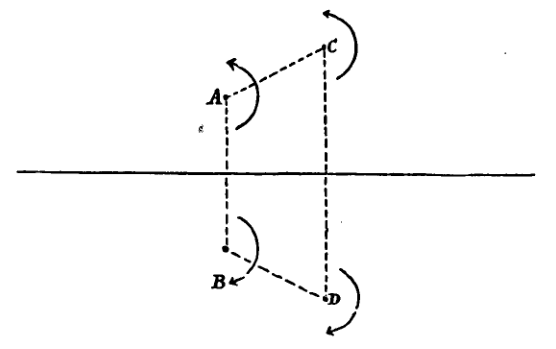
\includegraphics[width=\textwidth]{lovevort}
\caption{Point vortex pairs (A-B and C-D), from \citet[p.186]{love94}}
\label{fig:lovevort}
\end{figure}
If the vortex coordinates are
\begin{align}
\mbox{A:}&\hspace{0.5in}(x_0,y_0)\\
\mbox{B:}&\hspace{0.5in}(x_0,-y_0)\\
\mbox{C:}&\hspace{0.5in}(x_1,y_1)\\
\mbox{D:}&\hspace{0.5in}(x_1,-y_1)
\end{align}
and they have strengths $k$ (A and C) and $-k$ (B and D), then the motion of the fluid can be described by a streamfunction
\begin{equation}
\psi(x,y)=\frac{k}{2\pi}\ln\left(\frac{(x-x_0)^2 + (y+y_0)^2}{(x-x_0)^2 + (y-y_0)^2}\right) + \frac{k}{2\pi}\ln\left(\frac{(x-x_1)^2 + (y+y_1)^2}{(x-x_1)^2 + (y-y_1)^2}\right)
\label{eq:lovesf}
\end{equation}
\citep{love94}.

Now, with the aim of using the definitions of the streamfunction (\cref{eq:sf1,eq:sf2}), we differentiate \cref{eq:lovesf} with respect to $y$
\begin{align}
\partial_y \psi = \frac{k}{\pi}&\left(\frac{y+y_0}{(x-x_0)^2 + (y+y_0)^2}-\frac{y-y_0}{(x-x_0)^2 + (y-y_0)^2}\right.\nonumber\\&\left.+\frac{y+y_1}{(x-x_1)^2 + (y+y_1)^2}-\frac{y-y_1}{(x-x_1)^2 + (y-y_1)^2}\right),
\label{eq:lovesfdy}
\end{align}
and with respect to $x$
\begin{align}
\partial_x \psi = \frac{k}{\pi}&\left(\frac{x-x_0}{(x-x_0)^2 + (y+y_0)^2}-\frac{x-x_0}{(x-x_0)^2 + (y-y_0)^2}\right.\nonumber\\&\left.+\frac{x-x_1}{(x-x_1)^2 + (y+y_1)^2}-\frac{x-x_1}{(x-x_1)^2 + (y-y_1)^2}\right).
\label{eq:lovesfdx}
\end{align}
Now, we wish for the velocity of the vortices, i.e. we are looking at the above equations when $(x,y)\rightarrow(x_0,y_0)$ (or $(x_1,y_1)$).
Again following \citeauthor{love94}, we remove the terms that become infinite in this limit, thus obtaining,
\begin{alignat}{3}
\frac{dx_0}{dt}&=u_x (x_0,y_0)&&= \frac{k}{\pi} \left( \frac{y_1-y_0}{(x_0-x_1)^2 + (y_0-y_1)^2} + \frac{y_0+y_1}{(x_0-x_1)^2 +(y_0+y_1)^2} + \frac{1}{2y_0}\right),\label{eq:vortm1}\\
\frac{dy_0}{dt}&=u_y (x_0,y_0)&&= \frac{k}{\pi} \left( \frac{x_0-x_1}{(x_0-x_1)^2 + (y_0-y_1)^2} + \frac{x_1-x_0}{(x_0-x_1)^2 +(y_0+y_1)^2}\right),\label{eq:vortm2}\\
\frac{dx_1}{dt}&=u_x (x_1,y_1)&&= \frac{k}{\pi} \left( \frac{y_0-y_1}{(x_1-x_0)^2 + (y_1-y_0)^2} + \frac{y_1+y_0}{(x_1-x_0)^2 +(y_1+y_0)^2} + \frac{1}{2y_1}\right),\label{eq:vortm3}\\
\frac{dy_1}{dt}&=u_y (x_1,y_1)&&= \frac{k}{\pi} \left( \frac{x_1-x_0}{(x_1-x_0)^2 + (y_1-y_0)^2} + \frac{x_0-x_1}{(x_1-x_0)^2 +(y_1+y_0)^2} \right).\label{eq:vortm4}
\end{alignat}

\citet{acheson00} generalised these equations for a system of $N$ vortices (with strengths $k_1,k_2,\ldots ,k_N$), obtaining
\begin{align}
\frac{dx_i}{dt}&=\sum^N_{\substack{j=1\\j\neq i}} k_j \frac{y_j - y_i}{(x_i - x_j)^2 + (y_i - y_j)^2},\label{eq:vortposx}\\
\frac{dy_i}{dt}&=\sum^N_{\substack{j=1\\j\neq i}} k_j \frac{x_i - x_j}{(x_i - x_j)^2 + (y_i - y_j)^2},\label{eq:vortposy}
\end{align}
for $i=1,2,\ldots, N$.
The summations in \cref{eq:vortposx,eq:vortposy} are implemented in \hyperref[vortexf]{\texttt{vortexf.m}} and \hyperref[vortexg]{\texttt{vortexg.m}} respectively.

\section{Conserved Quantities}
Returning to \crefrange{eq:vortm1}{eq:vortm4}, and again following \citeauthor{love94}, we can express the right hand side of each equation by the partial derivative of some function $\chi$ (related to the streamfunction $\psi$), with respect to one of the vortex coordinates $x_0,x_1,y_0$ or $y_1$.
\citeauthor{love94} says the differential equations can ``clearly'' be put in the form
\begin{equation}
\frac{dx_0}{\partial_{y_0}\chi}=\frac{dy_0}{-\partial_{x_0}\chi}=\frac{dx_1}{\partial_{y_1}\chi}=\frac{dy_1}{-\partial_{x_1}\chi}=dt.
\label{eq:lovechi}
\end{equation}
To find this function, we must integrate the right hand side as follows:
\begin{itemize}
\item For \cref{eq:vortm1}, we integrate with respect to $y_0$:
\begin{align}
\chi &=\frac{k}{\pi}\int \frac{y_1-y_0}{(x_0-x_1)^2 + (y_0-y_1)^2} + \frac{y_0+y_1}{(x_0-x_1)^2 +(y_0+y_1)^2} + \frac{1}{2y_0}dy_0\nonumber\\
&= \frac{k}{\pi} \left( \int  \frac{y_1-y_0}{(x_0-x_1)^2 + (y_0-y_1)^2} dy_0\right. \nonumber\\ &\left.+ \int \frac{y_0+y_1}{(x_0-x_1)^2 +(y_0+y_1)^2} dy_0 + \int \frac{1}{2y_0}dy_0\right)\nonumber\\
&= \frac{k}{\pi}\left(\inv{2} \ln y_0 -\half \ln((y_0-y_1)^2 +(x_0-x_1)^2)\right. \nonumber\\ &\left. + \half \ln((y_0+y_1)^2 +(x_0-x_1)^2) +C_1 (x_0,x_1,y_1)\right)\nonumber\\
&=\frac{k}{2\pi}\ln y_0 \frac{(y_0+y_1)^2 +(x_0-x_1)^2}{(y_0-y_1)^2 +(x_0-x_1)^2}\cdot C_1 \label{eq:chi1}
\end{align}
\item For \cref{eq:vortm2}, we integrate the negative with respect to $x_0$:
\begin{align}
\chi &=-\frac{k}{\pi}\int \frac{x_0-x_1}{(x_0-x_1)^2 + (y_0-y_1)^2} - \frac{x_0-x_1}{(x_0-x_1)^2 +(y_0+y_1)^2} dx_0\nonumber\\
&= -\frac{k}{\pi} \left( \int  \frac{x_0-x_1}{(x_0-x_1)^2 + (y_0-y_1)^2} dx_0\right. \nonumber\\ &\left.- \int \frac{x_0-x_1}{(x_0-x_1)^2 +(y_0+y_1)^2} dx_0 \right)\nonumber\\
&= \frac{k}{\pi}\left(-\half \ln((y_0-y_1)^2 +(x_0-x_1)^2)\right. \nonumber\\ &\left. + \half \ln((y_0+y_1)^2 +(x_0-x_1)^2) +C_2 (x_1,y_0,y_1)\right)\nonumber\\
&=\frac{k}{2\pi}\ln \frac{(y_0+y_1)^2 +(x_0-x_1)^2}{(y_0-y_1)^2 +(x_0-x_1)^2}\cdot C_2 \label{eq:chi2}
\end{align}
\item For \cref{eq:vortm3}, we integrate with respect to $y_1$:
\begin{align}
\chi &=\frac{k}{\pi}\int \frac{y_0-y_1}{(x_1-x_0)^2 + (y_1-y_0)^2} + \frac{y_0+y_1}{(x_1-x_0)^2 +(y_0+y_1)^2} + \frac{1}{2y_1}dy_1\nonumber\\
&= \frac{k}{\pi} \left( \int  \frac{y_0-y_1}{(x_1-x_0)^2 + (y_1-y_0)^2} dy_1\right. \nonumber\\ &\left.+ \int \frac{y_0+y_1}{(x_1-x_0)^2 +(y_0+y_1)^2} dy_1 + \int \frac{1}{2y_1}dy_0\right)\nonumber\\
&= \frac{k}{\pi}\left(\inv{2} \ln y_1 -\half \ln((y_1-y_0)^2 +(x_1-x_0)^2)\right. \nonumber\\ &\left. + \half \ln((y_0+y_1)^2 +(x_1-x_0)^2) +C_3 (x_0,x_1,y_0)\right)\nonumber\\
&=\frac{k}{2\pi}\ln y_1 \frac{(y_0+y_1)^2 +(x_1-x_0)^2}{(y_1-y_0)^2 +(x_1-x_0)^2} \cdot C_3\label{eq:chi3}
\end{align} 
\item For \cref{eq:vortm4}, we integrate the negative with respect to $x_1$:
\begin{align}
\chi &=-\frac{k}{\pi}\int \frac{x_1-x_0}{(x_1-x_0)^2 + (y_1-y_0)^2} - \frac{x_1-x_0}{(x_1-x_0)^2 +(y_0+y_1)^2} dx_1\nonumber\\
&= -\frac{k}{\pi} \left( \int  \frac{x_1-x_0}{(x_1-x_0)^2 + (y_1-y_0)^2} dx_1\right. \nonumber\\ &\left.- \int \frac{x_1-x_0}{(x_1-x_0)^2 +(y_0+y_1)^2} dx_1 \right)\nonumber\\
&= \frac{k}{\pi}\left(-\half \ln((y_1-y_0)^2 +(x_1-x_0)^2)\right. \nonumber\\ &\left. + \half \ln((y_0+y_1)^2 +(x_1-x_0)^2) +C_4 (x_0,y_0,y_1)\right)\nonumber\\
&=\frac{k}{2\pi}\ln \frac{(y_0+y_1)^2 +(x_1-x_0)^2}{(y_1-y_0)^2 +(x_1-x_0)^2} \cdot C_4\label{eq:chi4}
\end{align}
\end{itemize}
Combining \crefrange{eq:chi1}{eq:chi4}, we can see that, noting that $(a-b)^2 = (b-a)^2$, we must have, for all equations to be equal
\begin{align}
C_1&=y_1,\\
C_3&=y_0,\\
C_2&=C_4=y_1 y_2.
\end{align}
So, we have
\begin{equation}
\chi=\frac{k}{2\pi}\ln y_0 y_1 \frac{(y_0+y_1)^2 +(x_1-x_0)^2}{(y_1-y_0)^2 +(x_1-x_0)^2},
\label{eq:chifinal}
\end{equation}
which agrees with the result in \citet{love94}.

Now we have found $\chi$, we can use it (with \crefrange{eq:vortm1}{eq:vortm4}) to derive the conserved analogues of energy and momentum, as stated in \citet{love94}.
Equating the $dy_0$ and the $dy_1$ parts of \cref{eq:lovechi}, we have
\begin{align}
\frac{dy_0}{-\partial_{x_0}\chi} &= \frac{-dy_1}{\partial_{x_1} \chi},\\
\Rightarrow \frac{\dxb \chi\cdot dy_0 + \dxa \chi \cdot dy_1}{-\partial_{x_0 x_1} \chi}&=0,\\
\Rightarrow \dxb \chi\cdot dy_0 + \dxa \chi \cdot dy_1 &=0,
\end{align}
and, as
\begin{equation}
\dxb \chi = \dxa \chi,
\end{equation}
we have
\begin{align}
dy_0 + dy_1 &=0\\
\Rightarrow y_0 + y_1 &= \mbox{CONSTANT},
\end{align}
as in the paper.

Now equating the $y_0$ and the $x_0$ terms, we have
\begin{align}
\frac{dy_0}{-\dxa \chi} &= \frac{dx_0}{\dya \chi},\\
\Rightarrow \dya \chi dy_0 &= - \dxa \chi dx_0,\\
\Rightarrow \int d\chi &= - \int d\chi,\\
\Rightarrow \chi +c_1 &= -\chi + c_2,\\
\Rightarrow \chi &= \mbox{CONSTANT}.
\end{align}

\clearpage
\section*{Appendix I: MATLAB Code}\label{sec:ap1}
MATLAB code for the vortex leapfrogging program (\texttt{vortexleap.m}\normalfont) and subroutines (\texttt{vortexf.m}\normalfont,\texttt{vortexg.m}) are given below.
\subsection*{\texttt{vortexf.m}}
\label{vortexf}
\begin{verbatim}
function[fi]=vortexf(i,k,x,y,N)
fi=0;
jmat=[1:1:N];
jmat(i)=[];
for j=jmat
    rr=((x(i)-x(j))^2)+((y(i)-y(j))^2);
    fi=fi+(k(j)*(y(j)-y(i))/rr);
end
end
\end{verbatim}
\subsection*{\texttt{vortexg.m}}
\label{vortexg}
\begin{verbatim}
function[gi]=vortexg(i,k,x,y,N)
gi=0;
jmat=[1:1:N];
jmat(i)=[];
for j=jmat
    rr=((x(i)-x(j))^2)+((y(i)-y(j))^2);
    gi=gi+(k(j)*(x(i)-x(j))/rr);
end
end
\end{verbatim}
\subsection*{\texttt{vortexleap.m}}
\label{vortexleap}
\begin{verbatim}
clear all
N=input('number of vortices = ');
%set time step and scales
t=0;
T=input('number of time steps = ');
%set length step and scales
h=input('step-size = ');
%define vortex strengths
for i=1:N
    k(i)=input(['strength of vortex ',num2str(i),' = ']);
end
%define variable for position
x=NaN(1000,N);
y=NaN(1000,N);
for i=1:N
    x(1,i)=input(['x-coordinate of vortex ',num2str(i),' = ']);
    y(1,i)=input(['y-coordinate of vortex ',num2str(i),' = ']);
end
for a=2:T
    clear x1 x2 x3 x4 y1 y2 y3 y4 k1 k2 k3 k4 l1 l2 l3 l4
    x1=x(a-1,:);
    y1=y(a-1,:);
    k1=NaN(1,N);
    k2=NaN(1,N);
    k3=NaN(1,N);
    k4=NaN(1,N);
    l1=NaN(1,N);
    l2=NaN(1,N);
    l3=NaN(1,N);
    l4=NaN(1,N);
    for i=1:N
        k1(i)=h*vortexf(i,k,x1,y1,N);
        l1(i)=h*vortexg(i,k,x1,y1,N);
    end
    x2=x1+(k1/2);
    y2=y1+(y1/2);
    for i=1:N
        k2(i)=h*vortexf(i,k,x2,y2,N);
        l2(i)=h*vortexg(i,k,x2,y2,N);
    end
    x3=x1+(k2/2);
    y3=y1+(y2/2);
    for i=1:N
        k3(i)=h*vortexf(i,k,x3,y3,N);
        l3(i)=h*vortexg(i,k,x3,y3,N);
    end
    x4=x1+(k3);
    y4=y1+(y3);
    for i=1:N
        k4(i)=h*vortexf(i,k,x4,y4,N);
        l4(i)=h*vortexg(i,k,x4,y4,N);
    end
    x(a,:)=x(a-1,:)+((1/6)*(k1+2*k2+2*k3+k4));
    y(a,:)=y(a-1,:)+((1/6)*(l1+2*l2+2*l3+l4));
    percent=100*a/T;
    display([num2str(percent),'% done'])
end
clf
%for viewing evolution of tracks
%multicomet(x,y)
%for viewing static image of tracks
colourmap=['b','r','g','c','m','y','k'];
maxy=1.5*max(max(abs(y)));
hold on
for i=1:N
    plot(x(:,i),y(:,i),colourmap(i))
end
xlabel('x');
ylabel('y');
title([num2str(T),' time steps, step size = ',num2str(h)]);
axis([0 inf -maxy maxy])
hold off
name=input('file name? ');
print('-dpng',[name,'.png']);
\end{verbatim}
The scheme used is a fourth order Runge-Kutta method with non-adaptive step size. The equations plotted are from \citet{acheson00}.
\bibliographystyle{dcu}
\bibliography{kwnrefs}
\end{document}
